% Caraumã book template by @jndgomes
% 2024 (c) Janderson Gomes
% See more <artientista.blogspot.com> or <carauman.blogspot.com>

% paper size is in preamble.sty
\documentclass[12pt,openany]{book} 

% Definindo proporção áurea
\newcommand{\goldenratio}{1.618}

% Codificação de entrada e saída
\usepackage[T1]{fontenc}

% Informações do livro
\newcommand{\authorname}{Aeridinae Lunaris}
\newcommand{\booktitle}{Birthright}
\newcommand{\subtitle}{Valkyrie's Shadow I}
\newcommand{\publisher}{Ashurbanipal}
\newcommand{\editionyear}{2025}
\newcommand{\isbn}{}
\title{\booktitle}
\author{\authorname}

% Pacotes adicionais
\usepackage{../res/options}

% custom colors
\definecolor{background}{HTML}{69c5a0}
\definecolor{circles}{HTML}{ffffff}
\definecolor{middlecircles}{HTML}{288D8A}


\definecolor{title}{HTML}{ffffff}
\definecolor{author}{HTML}{033854}
\definecolor{subtitle}{HTML}{033854}

\begin{document}

% Front matter
\frontmatter
\pagestyle{empty}


% Capa
\begin{center}
\begin{tikzpicture}[remember picture,overlay]

    % Fundo preto
    \fill[background] (current page.south west) rectangle (current page.north east);

    % Autor
    \node[white, font=\Huge, anchor=north, text width=\linewidth, align = center] (author) at ([yshift=-44pt] current page.north) {\textcolor{author}{\scshape\large\authorname}};

    % Title
    \node[title, font=\Large, anchor=north, text width =0.9\linewidth, align = center, below=4pt of author.south] (title) {\scshape\Huge\booktitle};

    % Subtítulo
    \ifx\subtitle\undefined\else\if\relax\detokenize\expandafter{\subtitle}\relax\else
    {\node[white, font=\Large, text width =\linewidth, align = center, anchor=north, below=8pt of title.south] {\textcolor{subtitle}{\scshape\large\subtitle}};}
    \fi\fi

    \node[anchor=north, below=30pt of title.south] {
\includegraphics[width=0.8\textwidth,decodearray={1 0 1 0 1 0 }]{../res/AOG.png}};

    % Centeral Circles
    \begin{scope}[shift={(0, -0.55\paperheight)}, scale=1.0871]
        \foreach \x in {-20, -18, -16, -14, -12, -10, -8, -6, -4, -2, 0, 2, 4, 6, 8, 10, 12, 14, 16, 18} {
            \foreach \y in {-2, 2} {
                \begin{scope}[shift={(\x + 1, \y)}]
                    \foreach \r in {0.2, 0.4, 0.6, 0.8, 1.0} {
                        \draw[thick, circles] (0,0) circle (\r);
                    }
                \end{scope}
            }
            \foreach \y in {-3, -1, 1, 3} {
                \begin{scope}[shift={(\x, \y)}]
                    \foreach \r in {0.2, 0.4} {
                        \draw[thick, circles] (0,0) circle (\r);
                    }
                \end{scope}
            }
            \foreach \y in {-1, 1} {
                \begin{scope}[shift={(\x, 0)}]
                    \foreach \r in {0.2, 0.4, 0.6, 0.8, 1.0} {
                        \draw[thick, circles] (0,0) circle (\r);
                        %\fill[thick, background] (0,0) circle (\r);
                    }
                \end{scope}
            }
            \foreach \y in {-1, 1} {
                \begin{scope}[shift={(\x, \y)}]
                    \foreach \r in {0.2, 0.4, 0.6, 0.8, 1.0} {
                        \fill[background] (0,0) circle (\r);
                    }
                \end{scope}
            }
            \foreach \y in {-1, 1} {
                \begin{scope}[shift={(\x, \y)}]
                    \foreach \r in {0.2, 0.4, 0.6, 0.8, 1.0} {
                        \draw[thick, circles] (0,0) circle (\r);
                    }
                \end{scope}
            }
        }
    \end{scope}

    % Editor
    \node[white, font=\Huge, anchor=south] (publisher) at ([yshift=32pt] current page.south) {\textcolor{title}{\scshape\large\publisher}};

    % Editor Logo
    \node[anchor=north, above=4pt of publisher.north] {
\includegraphics[width=0.15\textwidth,decodearray={1 0 1 0 1 0 }]{../res/Momonga.png}};
    
\end{tikzpicture}
\end{center}

\cleardoublepage

% Página de título (contra-capa)
\begin{titlepage}
	\centering
	\newgeometry{top=1in,bottom=1in,right=0in,left=0in}
    \thispagestyle{empty}
	~	
    % Autor
	\vspace{24pt}
	{\scshape\large \authorname\par}

    % Título
	\vspace{6pt}
	{\scshape\Huge \booktitle\par}

    % Subtítulo
    \ifx\subtitle\undefined\else\if\relax\detokenize\expandafter{\subtitle}\relax\else
    {\vspace{6pt}
	{\scshape\large \subtitle\par}
 
	\vspace{\stretch{1.25}}}
    \fi\fi
    
    % Quem fez a tradução
    \ifx\translatorname\undefined\else\if\relax\detokenize\expandafter{\translatorname}\relax\else
    {{\itshape\large{Tradução por}\par}
	\vspace{6pt}

    {\itshape\Large\translatorname\par}}
    \fi\fi

    % Editora
    \vspace{\stretch{6}}
	{\Huge\scshape\large\publisher\par}
\end{titlepage}
    
{\small
\setlength{\parindent}{0em}\setlength{\parskip}{1em}
~
\vfill

Ashurbanipal Edition, \editionyear{}

% Copyright
Copyright \copyright{} 2021 \authorname

Here shouldst thou set the ‘license.’ But lo, this is a fan-born edition of fan fiction; wherefore should any license be here?

% ISBN, se houver
\ifx\isbn\undefined\else\if\relax\detokenize\expandafter{\isbn}\relax\else{ISBN \isbn{}}\fi\fi

% Logotipo da editora

\includegraphics[width=0.07\linewidth]{res/AOG.png}

% Editora
``Published'' by \publisher{}
}  
% Prefácio
\chapter{Preface}

In the wake of the Battle of Katze Plains, the banner of Ainz Ooal Gown flies proudly over the city of E-Rantel. The Sorcerous Kingdom has entered the world’s stage to the clamour of death and devastation; the surrounding nations fearfully prepare even as they reel from its calamitous debut. Within the borders of the newly annexed realm, its Human subjects cower in their homes as the Undead openly walk the streets and stalk the lands. Yet, when a destitute noble finds herself under the auspices of an unlikely benefactor, events are set into motion that will resound over the world for ages to come.

A kingdom builder based on the events and setting of Kugane Maruyama’s Overlord. In a fantasy world where beings of matchless power are transmigrated from the arbitrary existence of a game, Valkyrie’s Shadow chronicles the lives of the natives whose reality has been turned upside down by their advent. It is the tale of a nation created by the whims of a supreme sovereign, and his unstoppable servants who each have their own, often twisted, interpretations of their Master’s Will. 



There is no victory in strength; no miracles wrought from magic that will save them: only the inexorable advance of a new world order where those who secure a place of service within will find themselves turned against the world that they once knew.

\cleardoublepage   % Make sure contents page starts on right-side page        
\tableofcontents\thispagestyle{empty}\cleardoublepage 

% Main matter
\mainmatter
\pagestyle{fancy}                  % Estilo de página fancy para o conteúdo principal

% Conteúdo dos capítulos
\part{Prelude}


\chapter{Pandora's Actor}

\begin{figure}
    \centering
    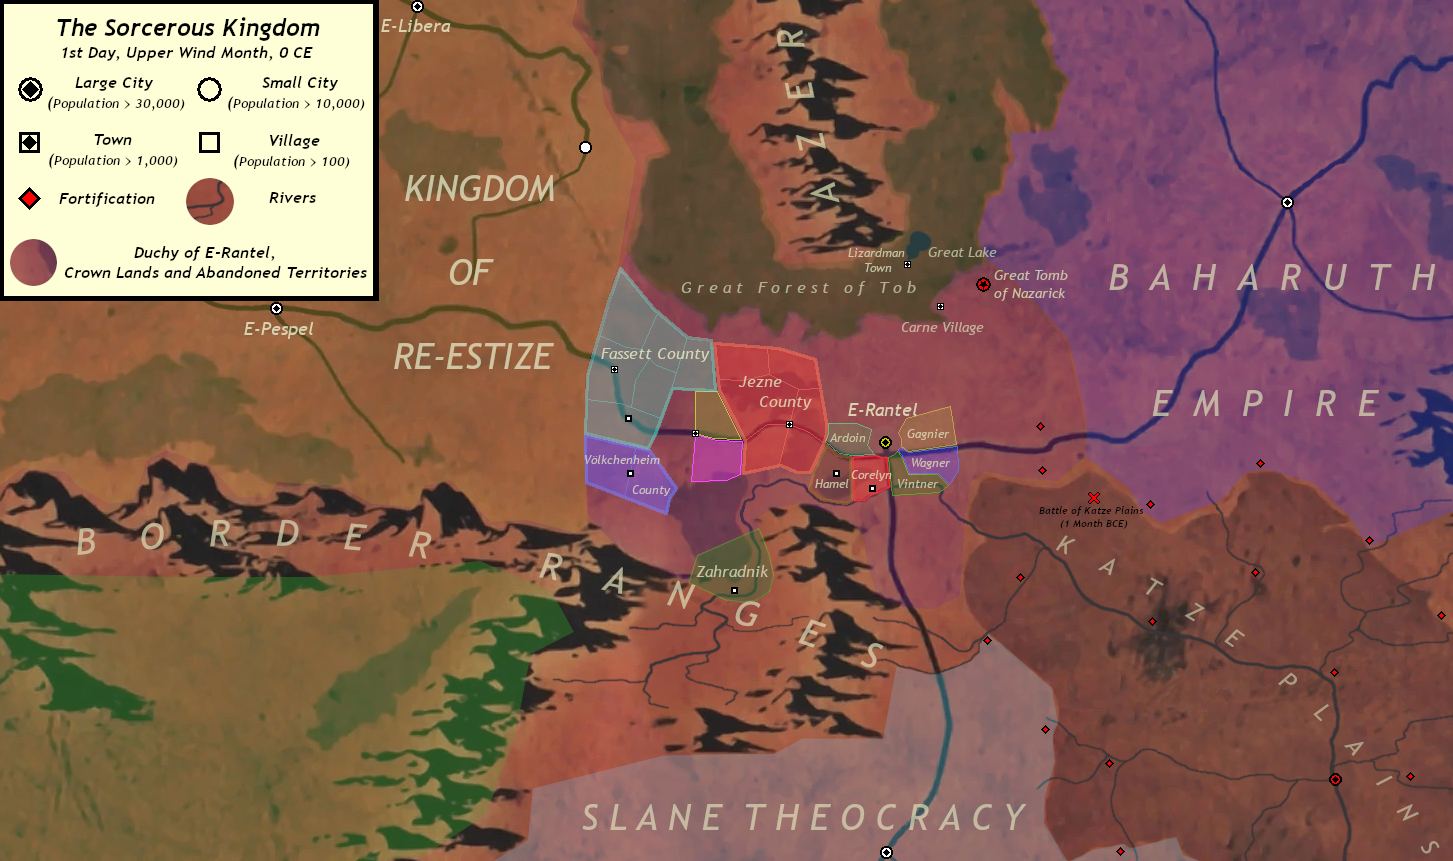
\includegraphics[width=1\linewidth]{images/ViGYZcC.png}
    \caption*{Political Map of the Sorcerer Kingdom}
\end{figure}

"Haaahhh~"


A prodigious sigh arose from behind him. It was a sound filled with equal parts annoyance, frustration and fatigue – as if one’s soul had been stretched thin and would dissipate like their misted breath in the frigid spring air. The drawn-out expression prompted the man to shift his body to look towards his companion: a woman seated astride a handsome mount that trotted after his own.

 

She was dressed plainly, in a clean set of traveller’s garments; wrapped in a brown cloak that tumbled past her horse’s flanks. Silky black hair – which somehow maintained its gleaming lustre despite long days of riding on rough country roads – was tied up in a loose ponytail that lightly streamed back and forth in the morning breeze. In her hands, she grasped an unfurled roll of parchment; her face was painted with an expression of irritation.

 

It gave an edge to her cold beauty, which – much to his own bemusement – had become something of a commodity in itself amongst some of the locals. Had he not known better, he might have assumed that it was the content of the parchment that was the source of her vexation...but he possessed a copy of it as well.

 

It was a map: a rough copy prepared from one that was found filed away in the civil offices of E-Rantel, detailing the southern regions of its duchy.

 

He had seen the original himself – its aged vellum cracked and yellowed despite careful attempts at preservation over the years: a meticulous survey done generations ago when the Kingdom of Re-Estize was near the height of its prosperity.

 

Laid upon it was a burgeoning frontier in the midst of expansion. The primal woodlands of the wilderness had been cleared away to make room for farms and pastures. Aristocratic manors spotted the fiefs on the map, carefully positioned on a network of well-travelled earthen roads. A multitude of hamlets and villages had sprouted up around them, filled with hopeful immigrants from the more populated regions of the Kingdom and beyond – pioneers cultivating the land to build a future of their own.

 

It was a map that spoke of a bright future. It was a time where order ruled and enterprising Adventurers tamed the wild borderlands surrounding the fledgling town that would grow to become E-Rantel, forging the way for settlement and industry. The House of Vaiself put its full support behind the expansion, investing heavily in both manpower and materials. When suitable lands were cleared, new titles were bestowed on those of appropriate merit, and so this cycle continued until the duchy had expanded all the way into the foothills of the border ranges to the south.

 

It was a map made generations ago; yet now, barely a trace of the scenery depicted by its features could be found in their surroundings. But it was not the feeling of betrayed expectations, he knew, that drew the heavy sigh from the woman behind him.

 

If she was aware of his gaze, she did not show any sign of it. She simply continued to scowl at the map as if her glare could ignite the thin piece of paper and scatter its ashes to the wind. Most likely, he mused, she was imagining the inhabitants: Humans, toiling in their simple fields and pastures; milling about in their meagre hamlets and villages. Tens of thousands of Humans squirming across the face of her map like a writhing infestation that threatened to crawl off the parchment, onto her fingers and up her arm.

 

He suppressed a smirk as he turned back around to face forward, though no one could have possibly seen it under the pitch-black metal of his fully-enclosed helm. While he did not exactly empathize with her feelings, as a fellow Doppelganger he understood the root of them.

 

The vast majority of their species nurtured a natural disdain of those not of their own, bordering on a malignant, almost xenophobic hatred. While their place as denizens of Nazarick meant that they got along well enough with fellow servants of the Supreme Beings, it also meant that outsiders earned a double serving of both a Doppelganger's natural ire and the sense that accompanied their existence as wretched, misbegotten creatures: unblessed by the touch of their Creators.

 

Personally, he did not lend himself much to these feelings, but he was still plagued by a mild irritation of a different sort that steadily grew as their journey progressed further.

 

To curb the inevitable wave of citizens fleeing at the news of Re-Estize’s catastrophic defeat on the Katze Plains, they had been immediately dispatched as Momon and Nabe: the Adamantite adventurers of Darkness. Their objective was to calm the rural population with their presence in an effort to stem the tide of refugees from crossing the borders.

 

When they had departed on their mission, gently rolling fields lay fallow through the winter, undisturbed after the autumn harvest. The roads leading west were well worn and everywhere evidence could be seen of rural products having been readied for delivery to the winter markets. Much of it had already disappeared, carried away by the desperate tide.

 

It had seemed like a straightforward task at first; the groundwork for their mission had been laid out by the magnificent foresight of their Master. The fame of Darkness had spread far and wide; their reputation beyond any conceivable reproach. The labourers that still remained around the villages unbent themselves from their labours to cheer and wave as they passed. Wherever they stopped, men and women would gather about them with hope and excitement; whenever they spoke, everyone would give their full attention and support.

 

Many of the wealthiest families in the fiefs that straddled the paved highway leading westward towards the Kingdom seemed to have already gotten wind of recent events and had fled the duchy out of fear, so they spent little time with the accompanying formalities as they visited the towns, villages and hundreds of hamlets spread out over vast stretches of rural land.

 

However, as their journey turned southwards and the days and weeks passed, the farmlands grew more sparse...as did the people supposedly tending to them. Fields and pastures transformed into grassland and meadows dotted with small groves of aspen and other poplars. Eventually, the lands along the roads could no longer be recognized as anything resembling fields and patches of young forest grew more prevalent. The wide, open roads had become little more than shadowed footpaths with sunlight filtering down through gaps in the thick web of branches overhead. At this point in their journey, these roads could just as easily have been mistaken for old animal trails amongst the dense undergrowth but for the fact that they were unnaturally straight.

 

The route that they currently travelled was marked on the map as part of a network of trails wide enough for wagons and carts, crisscrossing the landscape and linking the myriad farming communities leading through to the southern frontier. In reality, however, it had become more and more dilapidated and overgrown the further they travelled.

 

If not for Aura, who had ranged across the area with her own detachment weeks previous and later explained that the map was indeed correct – that the wilderness had simply reclaimed the land over time – he might have written it off as a whimsical fancy concocted by some blustering bureaucrat trapped behind a desk in the city. Even his Creator, who now styled himself Ainz Ooal Gown, marveled at the land's ability to restore itself to its natural state.

 

“Momon-san.”

 

A soft, dispassionate voice from behind roused him from his recollections. He raised his head to scan the surroundings ahead of them. Slightly off the path at the crest of the ridge that they were currently scaling, not ten paces into the forest, a small building stood overgrown and shadowed by creeping vines. It appeared to have sunk into the ground somewhat, or perhaps layers of humus had built up around it over the years.

 

“I see it, Nabe,” he slowed his mount to a stop as his companion followed suit. “What did they find?”

 

As if on cue, a figure materialized out of the dimly-lit undergrowth nearby to Narberal. It was one of the many Hanzos deployed alongside them, combing the terrain ahead as both an escort and a reconnaissance force for their mission. Narberal leaned forward to receive its report with thanks – without their tireless work, covering the entire region would have taken ages.

 

“It’s an old sentry post,” she stated flatly. “Abandoned years ago.”

 

“Umu,” he nodded, urging his mount forward once again.

 

They had come across similar sights all along their journey once they had left the immediate vicinity of E-Rantel. Though some places had been abandoned in fear by their inhabitants and those that ruled over them upon hearing of the Kingdom’s defeat at the hands of the Undead Sorcerer King, most recounted a tale that was decades in the making.

 

The region had seen great growth in the past, but at some point it had begun to stagnate for reasons unknown to the current population. Though she would probably not admit it personally, this concerned the Guardian Overseer and Albedo had gone to great lengths to pore over past tax and census records in an effort to discover the cause. She could only infer that when the region had grown to a certain size, the resources and manpower used to expand the Kingdom’s territory had to be diverted towards policing and maintaining the land and its influx of immigrants.

 

Over a stack of old archival tomes, she explained how after the first generation of settlers passed their lands on to their descendants, their burdens began to pile up at an ever accelerating rate. Expenditures for security against monsters, Demihumans and bandits grew until they could no longer be maintained by taxation. The militia could only man the largest of population centres and adventurers could only be afforded as a stopgap measure against the most apparent and dire of threats. Roads became wrought with hazards and commerce slowed to a crawl as the dangers increased. With the land no longer safe and prosperous, immigration had ground to a halt. Over the years, outlying settlements were abandoned in turn until only nature was left to reclaim what had been taken from it.

 

“Those inferior lifeforms should have never crawled out of their holes,” Albedo’s words dripped with equal parts venom and disdain. “No matter what they may aspire to, worms will always be worms: destined to squirm beneath the ground.”

 

This slow and steady decay continued until the present day, where they bore witness to the dismal end of the tale. As both the Guardian and curator of Nazarick’s treasury, it both shocked and appalled him that the Kingdom could let its territory and possessions reach such a decrepit state. What had initially been irritation slowly rose to anger within him at the sight of every abandoned farm and village; every rusted plough and collapsed cottage. He continued to fume as he looked upon the painstakingly laid out network of run-down roads choked by vegetation with their aged sentry towers fallen into disrepair and ruin.

 

At one point he had imagined the Great Tomb of Nazarick in such a state and it filled him with such fury that even Narberal, who was often teased for being oblivious by her sisters, could feel the rage emanating from him and surreptitiously scurried further down the trail – though she never knew exactly why.

 

Shortly thereafter, he reined in his feelings on the matter so Narberal would stop shying away from him, though they still simmered beneath the surface somewhere. He consoled himself with the fact that this land was now under the dominion of Ainz Ooal Gown, and under his Master’s guidance and protection it would soon be vaulted beyond its former glory and fashioned into something suitable enough to be called a possession of the Supreme Beings.

 

“Furthermore,” Narberal continued, “the settlement at the end of the trail still seems to be intact and occupied.”

 

Pandora’s Actor, who had fallen to brooding at the first piece of news, looked once again to the crest of the ridge with interest.

 

“Hoh…” this was unexpected, indeed. “So at the end of all these ruined farmsteads and forgotten paths, something still stands? Let us see what manner of people can endure where all others have failed.”

 

Articles both valuable and remarkable were of keen interest to Pandora’s Actor. Like his creator, he was a collector; the idea that something unprecedented lay just beyond the next hill was a tantalizing thought with the otherwise unremarkable journey that they had made. Though nothing in this world that he had witnessed so far could hope to compare to what lay within the vaults of Nazarick, to discover articles both exotic and rare – to catalogue and ascertain their value – was a pleasure in and of itself.
\chapter{Pandora's Actor}

As it turned out, nothing turned up to greet them as they crested the top of the ridge. No pastoral vistas; no bustling town arrayed before them on the other side. What they found on the other side was actually the edge of a deep gully, and only the frayed ends of a broken rope bridge remained on their side of the gap. Far below, hidden by the trees and brush laid bare by the brief passing of winter, he heard the trickling of water and little else but wind through the branches. No sign of the old road remained far away on the opposite side, but a rough path branched from the opening of the trail down a rocky course before disappearing into the trees below.

 

Pandora’s Actor debated whether he should simply leap across and try to find the remains of the road, as the Hanzos did not specify which route had led to their discovery. After a moment, he decided to descend down the rocky trail that seemed to have at least seen recent use. Swinging off of his mount, he unsummoned it as he landed lightly on his feet.

 

“Let’s head down,” he said. “Did the Hanzo report anything else about what lies ahead?”

 

Narberal shook her head as she followed suit, dismissing her own steed and taking a moment to straighten out her attire.

 

Pandora’s Actor turned his attention towards the trail again after receiving her negative response. Perhaps he should have had the Hanzo report to him directly; at least it would have been able to offer its thoughts to him so he would have a better idea of what lay ahead. Then again, hierarchy was important – he did not wish to deprive Narberal of her cherished role in their duty.

 

In the end, he felt that it was fine as long as he did not lose the trail and leapt down several dozen metres at a time. The manner by which he alighted on outcroppings of rock on the way to the bottom of the gully was greatly at odds with the apparent weight of his full plate armour and twin greatswords. Narberal cast Fly on herself and floated down after him. Within a few breaths, he landed with a shallow splash in the creek that he had heard from far above.

 

The rugged trail followed alongside the clear rush of water downstream, where daylight filled an opening in the distance. Narberal had gone ahead and her silhouette could be seen floating over the water where the creek left the trees, body slowly pivoting in midair as she surveyed her surroundings.

 

He joined her a minute later, casually striding out from under the branches and into the open air. The stream’s course continued a short distance before cascading sharply down a series of falls until it joined with a broad river. The trail that they had been following crossed the creek a few metres before the first dropoff. Some old, mismatched planks were laid across the shallows there to provide footing for travellers, held in place by large stones.

 

Now clear of obscuring forest, the trail offered a commanding vantage over the vista that lay before them. The river below cut deeply through the foot of the Southern Border Ranges, carving sheer, rugged cliffs several hundred metres high that towered over the far shore. Entering from between the cliffs to the southwest, it rounded a small, rocky hill at the head of the valley, flowing northwards until it passed where they currently stood. The river disappeared into a steep canyon to continue its journey towards the fertile lowlands.

 

A thick veil of morning mist shrouded the bottom of most of the wide vale that stretched up the river’s course, with only the crown of the distant hill visible in the far end. The forested slopes on the western side of the valley were not as imposing as the cliffs along the far shore, but still rose steeply enough to be considered impassable to the average Human. Beyond the river vale, the wilderness ranges rose in stark relief to the layer of fog over the valley floor, laced with fresh spring snows.

 

It was not surprising that Narberal had stopped to look around at this point – there was a wealth of information to take in instantly upon leaving the trees. Combined with the exposed nature of the trail, it was a perfect location to lay an ambush for the unprepared. Yet beyond the tumult of the falls and the rush of the wind that whistled past them on its way south through the valley, no challenge appeared.

 

His companion appeared to be unwilling to stand down from her vigil so he took the lead instead, following the narrow path down into the fog. It led the rest of the way down to the valley floor, where it joined with the riverbank. Though the trail they had been following saw signs of recent use, there was no trace of tracks leading through the wet sand.

 

The mist slowly dissipated as the morning advanced, though not yet to the point where he could see much beyond their immediate surroundings. The sound of the river current and the odor of damp vegetation filled his senses. The moisture hanging heavily in the air seemed to cling to his cloak and work its way into the joints of his armour. He did not particularly mind the conditions, but he couldn't imagine humans wanting to live in such an environment.

 

As he pondered this, Narberal soundlessly floated down beside him, wordlessly ending her enchantment. She shook her head as he looked to her questioningly.

 

“Only the hill ahead stands out in this fog,” she said. “I could make out little else.”

 

Her face held a neutral expression as she spoke. Even when with other denizens of Nazarick, she was ever succinct in her dialogue. He motioned for her to lead the way and followed her up along the shore of the river.

 

As their destination loomed into view, they slowed their rapid pace to take in the features of the rocky mound that rose before them.

 

The settlement reported by the Hanzo was little more than what it sounded. A bare handful of what were unmistakably hovels constructed of soil, wooden panels and loose stone were built into narrow terraces cut from the hillside. There were few proper buildings that could be seen: aside from the crude manor built halfway up the ascent, which also seemed to be built into the hill like the rest of the homes that could be seen, there was another that looked to be a small warehouse below it. An unremarkable stone shrine stood at the top of the hill and a simple pathway laced haphazardly with rocks of various sizes wove its way down from the shrine, through the buildings and onwards towards the pebbled beaches of the riverbank below.

 

From the manor halfway up the hill, a wisp of blue-grey smoke rose lazily into the air. Pandora’s Actor spotted a person’s face in the window looking straight down at them, but before he could raise his hand in greeting, it vanished behind thin curtains.

 

“Tsk.” Narberal clicked her tongue in annoyance to his side – the first-hand confirmation of the settlement being inhabited had visibly soured her mood.

 

As the pair approached the point where the path from the settlement disappeared into coarse sand, the door of the manor swung inwards. From their vantage at the bottom of the hill, they could see the head of a spear appear from the shadow of the doorway. Before it could clear the entrance, however, it jerked unexpectedly and fell to the floor with a clatter. He pondered whether Momon would have stepped forward to assist this apparently troubled individual, but, unable to see what he was dealing with, he decided to stay beside Narberal at the edge of the village.

 

Eventually, the spear rose again, its head wobbling in the air as it was lifted back up. It finally left the doorway, carried by what appeared to be a giant bolt of fabric. Any remaining semblance of tension slowly turned into impatience as the caricature took several minutes to descend the path down to where they stood.

 

As it turned out, the curious figure was the same person that they had seen in the manor window upon their arrival: an adolescent human girl who could be no older than her mid-teens. Perhaps older? Unlike the concretely-defined existences created by the Supreme Beings, these strange peoples were so variable that he and the others often found it difficult to discern their qualities from outward appearance alone.

 

She was wearing a gambeson that was most certainly meant for a much larger man, which resulted in the thick, padded layers giving her the odd appearance he had noted as she made her way down. Its hem hung down past her knees and the absence of a belt caused the entire weight of the suit to hang heavily upon her shoulders. Loose strands of dark chestnut hair poked out from under a simple leather cap that was strapped onto her head. The girl slowed to an unsteady stop before them; the panicked trek down the hillside in the ill-fitting and oversized equipment having taken its toll on her slender frame.

 

However, as her gaze passed over them, the spear came up. Raised to her shoulder, the blade of her polearm was leveled directly at them.

 

To his side, Narberal bristled at the action and Pandora’s Actor quickly raised his hands in a disarming manner.

 

“We are Momon and Nabe of Darkness,” he announced in a calm and confident tone. “You may have heard of us.”

 

The fame of Darkness had spread far and wide; many people throughout this land could even recognize them on sight. But far out on the isolated frontier of what was formerly the Kingdom of Re-Estize, it was possible that they were entirely unheard of. In that case, they were simply a pair of dangerously armed and imposing strangers that had suddenly appeared out of the mist with no prior invitation or warning.

 

Seeing that the girl did not lower her guard, he cleared his throat and shifted into a less aggressive stance to continue.

 

“As you may know,” he said, “this duchy has come under the dominion of the Sorcerous Kingdom as a result of the battle at Katze Plains. We have come to deliver a missive from the capital to all landed nobles of E-Rantel. Is Bar…”

 

The voice of Momon trailed off in the midst of his delivery. Pandora’s Actor sensed that something was off.

 

Throughout what he gauged to be a relaxed and casual introduction, the waves of alarm and fear coming off of the girl had not subsided. He quickly reviewed the scenario in his mind, seeking out faults in his own performance. Then, with a start, he realized that he had let down his guard.

 

As he had shifted his body, the girl had maintained her crude stance. Yet the head of the spear did not follow him – the much larger and more threatening in appearance between the two Adventurers – as he moved. It remained leveled at the source of her fear.

 

At Narberal.

 

Als Tiger gesprungen und als Bettvorleger gelandet!

 

The idiom came to his mind unbidden and it took substantial effort to not blurt it out aloud.

 

When he had initially received his role as Momon, he believed it to be the perfect opportunity to employ his skills in the service of his creator – the perfect casting. Thrust onto a stage where he was showered with the praise and adoration of the citizens, he had employed his natural abilities as a Doppelganger to draw from the hopes and expectations of the people. By doing so, he was able to enhance his performance and drive the already legendary image of The Dark Warrior to ever greater heights. It was a simple task by his own estimation, yet at the same time supremely gratifying to fulfil a role that he had been seemingly born for.

 

As they entered lands that were increasingly abandoned, however, he had lapsed in the use of these powers with no audience to witness his performance. The result of this misstep was that an irregularity had slowly approached them in plain view, coming within striking range without him even being aware of the threat that she represented. He counted it fortunate that the witnesses to his mortifying oversight were few.

 

Resolving to salvage this unacceptable development, he immediately reached into the mind of the girl standing before them to skim her thoughts with his abilities. While he believed that there was little chance this young human presented any direct physical threat to either Narberal or himself, there was still the matter of what was causing her distress and how it could lead to affect some imperceptible future.

 

It did not take long to recognize the initial sensation; he had felt this fear before. Just a few days ago, after weeks of practice on the field, he had teleported back to E-Rantel to play his part in his Master’s triumphal entry into the city. It was the same emotion that rode through the Human onlookers when the Sorcerer King first entered E-Rantel. A fear born of horror; a terror that either paralyzed one where they stood, or drove them to act. To fight; flee – do anything to survive. A primal fear reserved for the monsters and inhuman enemies that lurked beyond the safety of their cities and villages.

 

Yet Narberal did not hold such an appearance. By Human measure, she was a woman whose sharp manner and exotic features exuded a cold beauty that drew the admiration and envy of all who encountered her.

 

Pandora’s Actor frowned at the incongruity as he navigated the waves of the girl’s overpowering emotions back into her mind until he could finally look out from her thoughts. Normally, it would be a challenge to read anything beyond surface thoughts, but in her distressed state the girl was laying her mind bare to psionic intrusion: the undisciplined mind of a low level individual, broadcasting her fear-ridden thoughts to any who would care to peruse them.

 

His field of vision lowered; he saw the haft of a spear and the gloved hand that held it fearfully directed at its target. Ragged, heavy breathing caused the tarnished blade to rise and fall unsteadily. Beyond his own figure, standing slightly to the side, the weapon was pointed directly at his companion.

 

Above the simple traveller’s garb covered by the plain-looking brown cloak was a smooth, pale visage that looked directly back at her with empty eyes. Despite being devoid of features, a withering aura of hostility could be felt coming from her. After lingering for a moment, he noticed what should have been Narberal's Human appearance faintly superimposed over her natural face. A quick note of Narberal’s hand showed that she still had her Ring of Non-Detection equipped…

 

Pandora’s Actor withdrew from the girl’s thoughts and gathered his own. Enchantments that allowed the recipient to pierce through illusions, defeat magical concealment and even see through abilities that changed one’s form were not unheard of – many casters within Nazarick were capable of the spell which replicated the effects of this sense. As part of his preparations in assuming the role of Momon, he had pored over the information collected since their arrival in this strange new world for any threats that could foil his guise.

 

Amongst the Humans of this world that they knew of, there were scant few. The closest, according to the reports, was a Cleric based hundreds of kilometres away in the royal capital of Re-Estize. Even then, the frightened girl standing before them did not match her description. No matter which way he looked at her, this young girl in ill-fitting armour had neither the bearing of a bold Adventurer, nor the vestments of a distinguished member of a priesthood, nor the appearance of a powerful – by the standards of this world – mage.

 

If anything, this girl resembled nothing more than an ordinary Human: one they could have encountered anywhere along their travels. It was a thought that sent a cold tendril of anxiety down his back over what could have been.

 

There were many mysteries in this world that they had suddenly found themselves in; things unheard of in Yggdrasil. This girl appeared to be one of them: something the Humans in the surrounding regions referred to as a 'Talent Holder'. They were exceedingly uncommon and usually never completely identical to one another. In fact, an individual that manifested such an ability was not guaranteed that it would ever be applicable in their ordinary lives. She may even have gone her entire life without realizing her own Talent; Re-Estize as a nation was, to be nice about it, not very advanced in terms of magic – her daily interactions would not have had her see very much more than her fellow Humans.

 

However, that would no longer be the case. The machinations of his Master would soon give rise to a nation of unprecedented mystical might; a nation filled with a multitude of peoples that would quickly render her Talent self-apparent. That this girl ended up with an ability that she could make immediate practical use out of meant that she was a proverbial diamond in the rough. Whether she could be used to forward his Master’s goals, however, was yet to be seen.


A rare item indeed, thought Pandora’s Actor as he raised a gauntleted hand to his helmet.

\part{Act 1}


\chapter{Ludmila Zahradnik}

“‘Twas a chill night, wasn’t it miss?” A cheery voice piped up beside her.

 

Ludmila looked to her side: the owner of the voice was a young woman who occupied the space in the hold beside her. Both her auburn hair and light spring blouse fluttered loosely in the wind as she juggled her nursing child from one side to the other. Ludmila’s mantle shifted slightly as she turned, and she offered a smile as she responded.

 

“Yes, the river is always chilly,” she said, “but we’re well into the spring now, so it won’t be so cold in the Vale.”

 

The sound of men and women beginning to stir from the shivering groups that they had huddled into for the night rose as the morning sun finally crested the ridge of peaks to the southeast. On the other side of her, Aemilia was putting away the blankets they had brought for the trip – which had ended up being lent to the people around them instead. The woman, along with her husband and child, had received Ludmila’s.

 

“Isn’t your first time, then?” The woman asked, “Sounds like you know how things are like out there.”

 

“I was born and raised there; I’ve just been away for a couple of weeks.”

 

“The gods must have sent you to help us, then,” her free hand moved in a reverent gesture. “I can’t imagine how things would have been if we hadn’t met you. Thanks again for lending us your cover.”

 

“It’s no problem, a good mantle is enough for this time of the year. I was worried more for you and your baby – it seems most of the passengers here weren’t ready for the weather.”

 

“Aye, seems so,” the woman agreed. “Don’t think we got any warning of it.”

 

Ludmila nodded lightly before she turned away, after which her smile slowly faded. Though she had been entirely occupied recently, she thought that she had adequately covered her responsibilities as an administrator. Now that she was on her way home and able to witness her work personally, however, she noticed various oversights; things she could have done better everywhere she turned – even before she actually arrived in her fief.

 

As the young mother had indicated, the migrants to her territory were ill-prepared for the journey; after a brief period observing the other passengers, Ludmila figured that they were ill-prepared for life in the highland valley as well. She had experienced the issue once already when Aemilia first came with her to her home, but for some reason it had never occurred to her to warn of the conditions that the migrants would experience before summer fully set in.

 

Watching her hopeful new subjects shiver in the cold as they huddled together between the cargo in the hold that night made her feel woefully inadequate. That she had even erred in such a simple matter felt outright neglectful in her responsibilities as their liege.

 

She felt a nudge at her arm and looked down to see an early lunch being offered by Aemilia. It was a meal prepared by Terah: between the food she set out for dining in the manor – which seemed standard for the nobles of the city – and the food that she packed for travel, it seemed that her Housekeeper was far more skilled at making the latter for some reason. It was so much better than the standard fare that she often requested her sandwiches and baskets for regular dining over the local cuisine.

 

Ludmila accepted the offered meal with thanks, and continued to observe the ship and their surroundings. Beyond Aemilia, the Linum family sat together in the hold: Lluluvien and Wiluvien with their mother between them. There was no sign of Ilwé’s condition having improved since being separated from Count Fassett. The dozen or so other passengers were all in the forward areas of the ship, putting the cargo in the hold between the Undead crew and themselves. Ludmila instructed her maids to not act in a deferential manner towards her on the trip, and had them all dress in common clothing to blend in and interact with the new migrants.

 

Three of the families were from the list of prospective tenants provided by Bishop Austine, while the fourth family was that of a journeyman weaver who had been contacted through the Merchant Guild. There were two farmers, as well as a cobbler, and the four families would eventually join the farming village undergoing reconstruction as more homes were constructed. For the time being, they would stay in the administrative village, using the vacant residences in the hill. There, they would receive orientation for life out on the frontier, as well as familiarization with Undead labour.

 

A low murmur rose as they sailed out of the gorge and the vista of Warden’s Vale opened up before the passengers. Spring had fallen fully over the verdant highland valley, and blossoms filled its flooded marshes and slopes. Ludmila, as usual, was looking out for changes rather than solely appreciating the natural beauty of her fief. To even a casual observer, her gaze would have probably held a tangible edge; Demihumans from the wilderness had been reported encroaching on the land, and she focused her attention fully with this idea in mind.

 

A conflicted feeling had risen from within her at the news: duty had called her far to the west and, shortly after answering that call, other duties demanded her attention in the south. While she relished in her solidified sense of purpose, at the same time she could not be everywhere at once. There was the Adventurer Guild as well…she wondered just how far behind she had fallen, and how they would treat her extended absence from her commitments with them.

 

A little over two hours later, she spotted the first problem as they pulled into the harbour. Rather than damage incurred by Demihumans or anything overtly threatening, this problem took the form of two tents on the flats where her ever-growing glut of timber stockpiles were laid out. It was something entirely unexpected, and she could not for the life of her figure out why the tents were there. They appeared to be stitched together from a patchwork of rough, undyed fabrics. A few men and women sat around a campfire as the boat sailed by.

 

Ludmila’s puzzled gaze lingered over the group before turning to the pier as the vessel made its landing. Nonna awaited at the shore with a clipboard in hand; the tome that she carried everywhere was placed into a small satchel slung over her shoulder. The points of crimson light in her skull did not appear to follow Ludmila as she hopped onto the wooden planks and approached, instead intent on watching the migrants preparing to disembark.

 

“Report to the manor after you’re done here,” Ludmila said as she walked by the Elder Lich.

 

As much as she wanted to ask about the unexpected arrivals right then and there, Nonna had her own work to do and Ludmila was loath to interrupt the exchange of cargo. Her single vessel was not nearly enough to keep up with the goods awaiting transport, and she didn’t want to personally make things any worse.

 

She made her way up the hill, stopping to check on the homes along the way. Upon finding vacant dwellings, one of her fears was put to rest. Her initial thought was that she had somehow committed an error while issuing her orders from E-Rantel, which had resulted in a shortage of accommodations for incoming migrants. Nonna would most likely be able to explain what was going on with the people at the tents. Continuing on her way, she stopped at the warehouse.

 

“Ah, Lady Zahradnik,” Jeeves greeted her as she appeared in the entrance. “Welcome back.”

 

The small Skeleton in his curious outfit bowed in greeting beside his lacquered black box. Within the warehouse, the aisles of shelves were partially filled, but the absence of dust overall indicated that things were being moved around regularly.

 

“Thank you, Jeeves. How are things going here?” She asked, “Have you identified any problems?”

 

“Inventories are flowing according to the schedules that you’ve outlined,” he replied. “There have been no additional demands beyond the projections…though our exports are being severely throttled – we still have plenty of space for storage on the flats below, but I am uncertain if it will be sufficient for the long term.”

 

“The supply of timber is solely from the clearing being done for the areas slated to be developed into farmland,” Ludmila said. “Once we’re finished there, the amount you see coming in should be drastically reduced. I don’t plan on stripping the valley bare, though I do intend to set aside an area for growing and harvesting trees at some point.”

 

“I understand,” Jeeves nodded. “If that is the case, then there should be no problem. Aside from that, a villager who came by informed me that a few strangers had been going around procuring cloth from the residents…I am uncertain what for.”

 

“That must be how those people below got the material for their tents – have you heard anything about what’s going on with them?”

 

“Unfortunately, I do not,” the Skeleton shook his head. “They have not come to interact with the village inventories at all. As far as I know, they have only been dealing with the Human residents.”

 

“I see…” Ludmila took one last look around the warehouse, “You’ve done well so far, Jeeves: don’t hesitate to inform me of anything you think requires my attention.”

 

Jeeves straightened at her words and smiled. At least she thought he smiled: without flesh it was impossible to tell for sure. His overall image, however, seemed to convey the idea that he was pleased.

 

“It is an honour to be of service, my lady,” he bowed, “have a pleasant day.”

 

Exiting the warehouse, Ludmila continued on her way. Following the ring of hammer on anvil, she soon found herself looking over the space where Ostrik Kovalev continued his labours. The smith was still working out of the portable forge which he had brought with him to the barony, but the workspace around him had changed drastically. A makeshift roof had been constructed over a length of the terrace, providing a warm and dry area to work under in relative comfort. Rows of crates filled with charcoal and bog iron were stacked in the spaces leading up to the forge itself, while beyond several bloomeries continued to burn as they smelted iron. There was also something else in the rear of the bloomery area which she had no idea about.

 

Four children scurried about the area – two boys and two girls – and one of them finally noticed her watching the whole operation as he came out to retrieve a basket of charcoal. He stared up at her with big blue eyes before running over to pull on the edge of Ostrik’s shirt.

 

“Whaddya want, kid?” He said absently as he continued to work.

 

The boy tugged more insistently, and the smith finally turned away from his work with a baleful gaze.

 

“Now listen here, you: I thought I–”

 

His voice cut off as he noticed Ludmila standing nearby.

 

“Lady Zahradnik,” he made to bow, wiping his hands on a cloth nearby, “I–”

 

“There’s no need to interrupt your work,” Ludmila said. “I just dropped by to see how things are going here.”

 

The smith nodded as he turned back to the forge, and Ludmila circled around to stand across from him nearby. Over the ledge of the rampart, she could see that nearly all of the piles being burned for charcoal were gone. The children continued about their tasks, tending to the clay bloomeries and keeping various parts of the workspace well stocked and clean. From her vantage, she could also see skeletal labourers pumping bellows attached to the furnaces.

 

“You’ve adjusted quite well here,” she noted. “You’ve even picked up a few apprentices.”

 

“With construction prioritizing the farming village,” he replied while waiting to reheat the piece he had been working on, “I figured I should make myself comfortable here. As for the kids, well…with as much as you seem to be planning on doing so far, I took as many as I thought I needed. I can’t say I could’ve taken any more though, we’ll need a bigger space for that.”

 

“I appreciate your initiative,” Ludmila said. “It was something I was going to approach you about sooner or later. Once the first village is done, there should be some time to construct a forge here while we wait for the woodsmen to clear away the next set of fields.”

 

“Ah, then, about that apprentice thing, my lady,” Ostrik said slowly as he resumed working. “There’s quite a bit of confusion as to how you plan on organizing your tenants.”

 

“How do you mean?”

 

“The way you’ve been running things here so far...how do I say it…” he said, “it’s uh, very controlled. For the time being, you’re providing for all of the needs of your subjects: food, clothing, sundries, fuel – everything. Nonna goes to visit the farming village twice a day, the villagers put in their requests, then Jeeves has the orders delivered via Bone Vulture or through a cart with those Undead Beasts if whatever they want is too heavy. Don’t get me wrong, I think it’s great: it’s all very orderly and clean and convenient, but it leaves your living subjects quite...detached, if I were to describe it.”

 

Ludmila furrowed her brow at the word. The system that she had devised was what she thought would be the best way to organize things based on the means she had at her disposal. Lady Shalltear had noted that it was a unique way of employing her resources, but Ludmila did not think she meant it in the way that Ostrik described. Her smith shifted uncomfortably and turned his gaze back to the forge.

 

“It’s, well…maybe it’s something like this,” he said. “The people are used to seeing shortages of things, or the price of services and goods to figure out how their little piece of the world is doing. It’s like that basically everywhere I’ve been. Here, though…here, you ask for something, and it arrives within an hour or two if it’s available. You put up goods for delivery, and something comes to pick it up and it disappears into the warehouse for Jeeves to take care of. They see all the timber harvested get carried by their homes and the ship goes up and down the river…but they really have no idea what is going on. Everything they do seems to vanish into an unknowable void, and that same void provides everything that they need.”

 

She thought over his words again, wondering what she could do to satisfy the lack which he described. Ostrik continued after completing the piece he had been working on, placing a new bar of iron into the forge.

 

“It was like that with the apprentices I picked up too,” he said. “Normally kids follow after their parents’ trade, and if their family has a feeling that they might not be able to survive doing the work for whatever reason they’ll try and send the kid off to apprentice in something that they think will work out.

 

“I was willing to take in those kids because I knew that you at least need this many – probably more – new smiths working eventually, but even so the things I have to figure out: how to provide for them, what to pay them when as they become more skilled in the trade, finding places for them to work…I really have no idea. Their room and board is provided for by you, so is their food and so is everything that they work with. This sort of formless future leaves people really wondering what’s ahead of them, and it can be quite frightening to some.”

 

“You understand that things are currently arranged the way they are due to the availability of goods and resources, yes?” Ludmila said, “My ability to provide for the population is limited at the moment, as there is only one ship transporting goods along the river – I need to keep our imports balanced to ensure the needs of the people are adequately addressed, so I can see how it can be perceived as my being…controlling. Even if I were to open a market in the village, however, the selection would be quite meagre.”

 

“Yes, I had a feeling it was like that, my lady,” Ostrik replied. “The people might understand that things are as they will be for a year or two as well. It might be because they’ve just moved in, or they’re being exposed to new things and getting used to life here…but they have the look of being lost beyond their immediate occupations. The things that they’re used to having as a gauge for how they are doing don’t exist, and there isn’t anything to show them where they fit within the framework of everything.”

 

“I see,” she said. “I believe I understand what you’re trying to say now…are you sure you aren’t some sort of Sage from somewhere?”

 

Ostrik laughed, shaking his head at her words.

 

“I’m no Sage, my lady,” he smirked. “Just a traveller.”
\chapter{Ludmila Zahradnik}

Ludmila left Ostrik to his work, stepping out from under the makeshift forge and into the light of the blazing sun overhead. It was plainly uncharacteristic weather for this side of the border ranges, especially in the transitions between winter and summer, which had the tendency to be overcast and wet. It wasn’t any mystery as to what was causing it, however.

 

Due to the slow start on the spring planting season, Lord Mare had altered the weather slightly throughout the duchy in order to ensure the crops grew and ripened on time. Well, it was slightly altered when it came to the lowlands, but the weather in Warden’s Vale had changed by quite a lot as a result of being downwind from everything. Ludmila’s territory only represented a small fraction of the land in the duchy, so she couldn’t reasonably ask Lord Mare to change everyone else’s weather on her behalf.

 

Between Lord Mare’s control of the weather and the magic he had cast over the fields once the crops were sown, her oats were easily on their way to meeting the harvest schedule with previously unheard-of yields. The implications were abundantly clear to all who bore witness to what would have been considered a miracle in their former nation of Re-Estize. Though magic being used to assist in agriculture was not a novel idea by any measure, the sheer scale at which it was employed in the Sorcerous Kingdom was unheard of.

 

Continuing her way up the village lane, she looked down towards the pier where Nonna was still overseeing the loading of timber. Once the summer harvest was ready for transport, Ludmila was not sure if her single vessel would be enough to transport all of the grain before the next harvest in the early winter.

 

The most straightforward solution was to build more ships, which was something Clara and Liane were looking into: a part of Clara’s long term plans for Corelyn Harbour was to include a shipyard to construct more vessels for the river trade. Another option would be to restore the bridge to reconnect her fief to the rest of the duchy by land. Doing so would be expensive, however, and nowhere remotely near as cost-effective as having more ships.

 

Voices on the terrace below drew her attention: the families that had arrived were being guided by villagers that had volunteered for orientation duties. She watched them silently from above, thinking of the issue that Ostrik had brought to her awareness.

 

Ludmila wasn’t sure if he honestly did not know what he was attempting to describe or simply trying to be polite, but what he had said amounted to there being a lack of purpose and leadership in the fief. In addition, despite its necessity for the time being, her control over the flow of goods made people feel powerless when it came to the smaller elements of their daily lives. With her continual absences from her own territory, Ostrik noted that new subjects were becoming more and more directionless. Thinking ruefully to the words she conveyed to Momon during their trip to E-Rantel, she supposed that it not only applied to kings, but leaders in general. She still wanted to thank the Adventurers of Darkness for their help, but she had not seen them since.

 

As for what she could do about the current state of her subjects, several solutions came to mind, some of which would probably manifest on their own at some point – such as the arrival of merchants when the population grew large enough. Ludmila’s long-term goals, however, were still relatively undefined. Her personal duties to Lady Shalltear did not really suggest what she should be doing with her own fief, and matters regarding taxes and other mundane contributions to her liege would need to be discussed before delivery of the harvest was completed. For the time being, she had settled on finishing the extension of farmland along the valley but, once the golems being used in the capital were free to lease, the schedule would be pushed forward rapidly.

 

She mulled over her options. Seeing that the boat had nearly finished loading, she strolled over to the manor entrance where a Death Knight stood sentry, as well as…something else. On the opposite side of the doorway there was a giant Demihuman with feline features, which was nearly four metres in length. Ludmila looked from the cat-thing to the Death Knight and back again: given that it wasn’t attacking and looked decidedly Undead, it should be something she could ask Nonna about when she received her reports. Giving it one last look, she shook her head and entered her home.

 

“Aemilia,” Ludmila called as she entered, “did you see that cat…thing…outside the door?”

 

“I did, my lady,” her maid replied. “It was just standing there, and the Death Knight didn’t seem to care so I just went in.”

 

“Did you hear anything about it on the way up here?”

 

“No, my lady. I just came in from helping the Linum family move in next door.”

 

“I see…how are they faring?”

 

“Lluluvien and Wiluvien are ecstatic – they already love the Vale. As for their mother…she is unchanged, as far as I can tell.”

 

Aemilia rounded up her Skeleton assistants and led them out of the door. Shortly after her lady’s maid had departed, Nonna appeared at the door. The Elder Lich placed several documents on her desk as Ludmila seated herself.

 

“Is there anything that requires my immediate attention?” She asked.

 

“Not at the moment, no,” Nonna replied.

 

“Then…what is that cat outside the door?”

 

“It is a Squire Zombie,” Nonna said. “Beings that fall to a Death Knight are raised as Squire Zombies under its control. Beings slain by a Squire Zombie will be similarly raised as Zombies under the Squire Zombie’s control.”

 

Rather than a cat bringing in its prey to display before its owner, the Death Knight had brought in a cat. Ludmila wondered if it would keep happening.

 

“I…didn’t know they could do that,” Ludmila said. “I assume this has something to do with the report of Demihumans encroaching on the border?”

 

“That is correct,” Nonna replied. “Several Demihumans of this species appeared on the borders of the fields several days ago. A pair of Bone Vultures intercepted them before they intruded too deeply, but they were destroyed. A Death Knight then arrived and dispatched one while the other Demihumans fled into the forest. This Squire Zombie is the result.”

 

“I don’t suppose anyone asked what they were doing here…can we ask the Squire Zombie?” Ludmila said.

 

“They approached in the middle of the night,” Nonna replied, “and the servitors were ordered to guard the fields. Death Knights utilize the corpses of the slain to raise Squire Zombies; they are not the same individual that was slain.”

 

Ludmila tapped her finger on her desk idly. The Undead Demihuman outside her door was not of a race she had ever seen before, so it was difficult to speculate as to why they had appeared. Still, the security of her demesne – and the border of the Sorcerous Kingdom – stood as a priority: one of her most basic duties.

 

“Then they performed their task as instructed. As requested by your report, I submitted the order for new Bone Vultures before I left the capital, so they should arrive at any time, if they haven’t already…were there any more encounters?”

 

“None,” Nonna said. “Though the Bone Vultures are currently the best detection assets we have deployed on patrol duties – they were unable to sense the approach of these Demihumans until after they left the trees and exposed themselves on the fields.”

 

This problem was something that Ludmila was already well aware of. Lady Aura’s rough outline of the Sorcerous Kingdom’s forces came to mind once again: there was a distinct shortage of forces that were capable of reconnaissance work beyond direct observation of subjects with poor concealment abilities. Trackers and other advanced detectors were relatively few, and Ludmila had resolved to train Rangers to make up for the shortfall in her own demesne – perhaps the nation’s armies would find a place for them as well. For the time being, however, she was the only Ranger in her fief.

 

“Was the Royal Court informed of the incursion?” She asked, “What did Lady Aura have to say?”

 

“The report is pending further investigation,” Nonna replied. “Would you like to inform the Royal Court immediately?”

 

“No, I believe you have the right idea,” Ludmila decided. “I don’t want to waste the Royal Court’s time – minor incidents are my responsibility to handle, anyways…before we move onto regular business, I have one more thing to ask: why are there tents outside?”

 

“Several Humans arrived without the proper authorization to migrate into the territory,” the Elder Lich answered.

 

“Without proper authorization?” Ludmila wasn’t sure what Nonna meant, “Did they stow away onto the ship in the past few weeks somehow?”

 

“They arrived overland yesterday. As they appear to be citizens, I thought it best to wait for you to render a decision on their...disorderly conduct.”

 

It barely took Ludmila a moment of thought to understand what had happened. She closed her eyes and sighed – yet another oversight.

 

“Indeed,” Nonna said. “Why must Humans move without orders? Such senseless and wasteful behaviour.”

 

Ludmila didn’t bother correcting the Elder Lich’s misinterpretation of her expression, as it was actually accurate in a twisted sort of way. The sensitive balance she was keeping in Warden’s Vale depended very much on the idea that people would only appear when she could provide for them. She had no expectations of people randomly arriving overland simply because it was close to unthinkable for common folk to make their way through the previously dangerous routes that led to her fief.

 

Under the rule of the Sorcerous Kingdom, travel within its borders was fairly secure unless one went somewhere they weren’t supposed to go – at which point security happened to you. His Majesty’s Undead armies had cleared away all of the hostile elements that could threaten its people along roads both new and old, so independent travel without personal protective measures was something that the people would eventually become accustomed to and expect.

 

“I’ll speak to them after we’re done here and find out what I can,” she finally said. “Hopefully this won’t become as large of an issue as I think it could be...”

 

The door opened, and Aemilia appeared with her skeletal assistants. Seeing her mistress at work, her lady’s maid quickly instructed the Skeletons to empty their buckets of water before going to the kitchen area to prepare tea.

 

“Speaking of immigration,” Ludmila looked back to Nonna, “there are several things that should be kept in the ship’s hold, just in case the new tenants are not prepared for the journey.”

 

Several minutes passed as she outlined improvements to the sparse accommodations on board the ship, as well as updates to be relayed to the manor in E-Rantel to deliver to the cathedral and Merchant Guild.

 

“This will reduce our cargo volume,” Nonna noted.

 

“It should only be a moderately sized crate, yes?” Ludmila replied, “A little bit of hospitality on the journey will help towards acclimating our new arrivals. Speaking of which, how goes the transfer of citizens to the village?”

 

“Due to the size of the residences ordered, each home takes roughly a week to build. Between them, the construction crews are raising homes at an average rate of one per day. The waiting time for new immigrants has remained stable as a result…do they really need such large accommodations? These buildings are far beyond the standard cottage size of the other rural fiefs observed in the duchy, not to mention the difference in material and construction quality.”

 

“I have a lot of space and not enough people,” Ludmila said as she shuffled through the summaries piled through her absence. “I am also competing with every other territory for skilled labour in this insane race to stay ahead of the deflating commodity prices. Being so far from civilization puts me at a marked disadvantage. If I want to bring civilization here, then civilization must look like it belongs here.”

 

Between the dusty dreams piled up in the manor archives – which consisted of what was in the small locked cabinet where the demesne accounts were held – and her own understanding so far of the strengths and weaknesses of the Sorcerous Kingdom’s forces, the layout she had plotted for the farming villages was ambitious: at least if one considered the duchy’s previous state as a territory of Re-Estize. With the availability of cheap Undead labour, all one needed was land and resources, which was something the mostly untapped expanse of her fief had plenty to spare. What resulted was a strange concept far removed from the traditional appearance of rural villages anywhere in the region.

 

Instead of a manor to house a member of the gentry or some sort of other Human administrative agency, Ludmila had instead come up with what she in the end had settled on calling a Lichtower. It consisted of several sections: the main, central part of the complex was an administrative office of two floors where she would station its namesake. The first floor would be used to service the villagers, while the second would house the village archives. Two wings were attached to store reserve Undead for the village if required, as well as provide space for future government facilities. The tower itself was twelve metres in height, providing a commanding view of the village’s surrounding farmland for sentries. Attached by a drawbridge, which provided access over the main road, was the warehouse office where parcels from Bone Vultures would be received and either transferred to the storage buildings nearby or picked up by awaiting residents.

 

The village itself was divided into two raised sections, which lay on their respective sides of the main road running through the farming terraces. On one side was the warehouse area, while the other housed the residents, services and essential facilities of the village. A small market square existed as well, but would probably not find any use until trade established itself. Both sections were enclosed in their own respective walls, which were connected to each other through gatehouses that straddled the road between the two parts of the village. Each entrance from the road into those sections also had a small gatehouse of its own.

 

When finally completed, the haphazardly constructed hamlet with its buildings strewn over a large area would be gone; in its place would stand an orderly and defensible farming outpost which rose over the fields. The village would house roughly 200 to 250 residents in its fortified enclosure: a stronghold which stood safe from sudden raids.

 

In any other place, it would be absurd to call it a village, and insanely expensive to construct. The fortifications were intended to shelter her subjects and the village’s goods, allowing the powerful Undead forces stationed there to focus on eliminating attackers as quickly as possible on the field. With the raw martial strength sufficient to handily destroy major cities in other nations being deployed by a single village, Ludmila deemed it more than enough to deal with anything short of a large army – which would probably become a matter of national security rather than something a farming village was expected to deal with.

 

The village was not without issues, though. As Nonna had stated, construction times were markedly slow in comparison with the much simpler construction that rural villages usually saw. Then there was the recent ordinance sent out by the central administration to harden crucial points in national logistics against attacks from both land and air. She also needed to somehow make them defensible against magic casters of the fifth tier. The latter was still something she was studying: slowly developing a grasp on the possibilities and potential applications of various forms of magic.

 

The initial concepts which went into the village were clearly only drawn up with defence against attacks from land in mind. Currently, with as little knowledge as she held in magic and aerial combat, her only solutions involved using brute force to overcome such attackers: throwing what she thought might be effective against various types of intruders. Hopefully, she could consult with Lady Shalltear – or perhaps Lord Mare – over these problems at some point. Beyond this, however, she was fairly confident that it would do what it was supposed to, and word would spread that her fief on the border was a prosperous and safe place to live as the seasons came and went.

 

“Besides,” Ludmila smiled lightly, “you agreed that the village layout was far superior to those of the inner territories, yes?”

 

“For all intents and purposes, before the new guidelines came in for fortifications,” Nonna affirmed. “Considering the tendency of you Humans towards disorderly conduct, however, I am dubious that the additional long term purpose of these settlements will work as you describe.”

 

The additional purpose Nonna referred to was essentially enforced by the limitations of each farming outpost. Each could normally support and house a set population within its walls, so the excess would be encouraged to migrate. Each would hold one of the future schools that Clara had described, as well as facilities to train apprentices in all the trades that went into supporting a small settlement. Ideally, it would raise successive generations of skilled workers with a basic standard education. A substantial portion of these new generations would move out due to lack of space, and the capital of her fief would by then be ready to welcome them.

 

“I do not expect everything to work exactly as planned,” Ludmila replied to Nonna’s doubts, “but it should work well enough. Our systems will always be subject to refinement, so we should always be on the lookout for ways to improve on the development of the demesne.”

 

Aemilia appeared from the back of the manor with tea, placing the simple wooden cup on the desk.

 

“I suppose that now is a good time to see to all of the petitions around the village,” Ludmila said. “Nonna: prepare a list of all the villagers in this settlement that have requested an audience in the time I’ve been away – I’ll hold court in the farming village tomorrow. Aemilia, check if the Linum sisters are settled in: if one of them is available, I’ll have her deliver my summons.”

 

Taking a careful sip out of the steaming cup in front of her, Ludmila settled in for a long afternoon of work.
\chapter{Ludmila Zahradnik}

At the gloomy outburst, Ludmila furrowed her brow in confusion and felt a hint of distaste well up within her. Frontiersmen were a subdued and practical lot – the men and women of Warden’s Vale were not prone to bouts of melodrama like some unskilled tavern bard.

 

“Lost? How?” She pressed Milivoj, “You should have barely arrived.”

 

For years now, the Kingdom of Re-Estize and the Baharuth Empire regularly held a large skirmish around the autumn harvest season. Neither side would purposely commit to pitched battle and the outcome was similarly indecisive. The casualties inflicted could barely be called damage: so tiny they were, compared to the nation’s population of over nine million. Each year, the great houses would play their games, and their vassals would try to figure out how to deal with all the logistical shortfalls it would cause.

 

In line with the rather late declaration of war by the Empire, the King had raised his banners over a month previous. Since it was an expected occurrence by this point, Baron Zahradnik had already long prepared his quota of men and supplies and left that same week. Going by Milivoj's statement and the unexpected return of the men, this outcome should have occurred only a handful of days after their arrival at E-Rantel – barely enough time to finish setting up their camps and preparing for the initial skirmishes.

 

Ludmila couldn't accept this claim. With both sides putting minimal effort into the battle, it should have been a standoff that played out over many weeks – well into late winter, perhaps even spring. That should have been the point, after all: the longer the Empire lingered at Katze, the longer the Kingdom’s levies would be prevented from participating in the regular activities of the season. The Autumn harvest had long been completed by the time the call to arms had been sent forth, so it seemed that the Empire had chosen to both stifle the busy winter trade and delay the spring planting season.

 

It represented an aggressive shift in the Empire’s strategy: delaying the bustling winter markets in the region would have meant supplies would not reach the fiefs that needed them. The planting season – if postponed for long enough – would require that crops and livestock be organized in a drastically different fashion to account for lost weeks of growth, if they could be at all. To Ludmila, this sudden move to throw the Kingdom off balance indicated that the Empire was about to change the way they waged war some time in the near future, but the idea that they would face such a drastically different result in the same year was beyond her ability to imagine.

 

“Milivoj, answer Mistress Ludmila’s question,” Bohdan spoke gently to the man, trying to coax him to speak further.

 

The priest leaned forward, laying his hands on the haunted-looking man. Ludmila did not hear any spells being cast, but Milivoj seemed to visibly gather himself and started to speak again in a clear and regular tone.

 

What followed was the account of a nightmare. It could be only that.

 

Milivoj’s eyes regained their focus as he finished his recollection, looking between Ludmila and Bohdan as he ended his account. He seemed oddly calm, as if sharing his memories had distanced him from his experience somehow. Ludmila shifted uncomfortably. There were so many points where she thought she should have questioned, but it was all so fantastical and horrifying that she had refrained from doing so as the young man spoke. Even now, she was at a loss as to how to proceed.

 

The tale was long, and the use of divine magic to eliminate Milivoj’s fear and force lucidity upon his mind resulted in an eerie, distant account that spared them none of its gruesome details. Some of those, she could not even begin to understand...or perhaps words were simply insufficient to do so. Tens of thousands of men, falling to the ground dead as if a giant scythe had swept through them like so much grain. Colossal globes of liquid darkness that rained over the field, birthing colossal, nightmarish creatures that could only be described in loose relation to more common things. The appearance of an Undead caster who possessed the might to control those unfathomable monsters.

 

She couldn’t even guess at how many lives had been lost in the carnage. It was beyond the comprehension of a teenage girl living out on the edge of civilization with a scion’s education and limited experience outside the borders of their isolated fief. Beyond what any of them knew. Even those villagers who had spent decades defending the border against the myriad of Demihumans and monsters from the wilderness had never recounted anything so bizarre, horrifying and deadly.

 

But…Bohdan might know. The venerable priest had lived long and seen much, undergoing his training as an Acolyte in the Theocracy. A mentor and friend who had long served the barony and its people with his divine magic and generations of wisdom. Ludmila turned to see if she could lean on his knowledge and experience, but her words caught in her throat as when she saw the ghastly expression painted on his worn face.

 

“...spare us.”

 

The elderly priest was the first to break the silence that followed, with words barely audible as they passed his pale, thin lips.

 

“May Surshana spare us,” his voice rose as he invoked the grace of the god of death. “The army of the Kingdom, destroyed. The Empire, fighting on the side of abominable horrors and evil Undead!”

 

His quivering voice continued to rise and Bohdan turned to face her. The feverish gleam in his eyes was so intense that she felt herself take a step back.

 

“Mistress Ludmila,” he said, “we must leave.”

 

Ludmila’s mouth opened and closed, and she looked back and forth between the two men. Motioning for the priest to hold, she turned to Milivoj, who remained leaning on the wall of his home.

 

“Milivoj, please get some rest,” she touched him gently on the shoulder. “I’m sorry for asking you to remember all of that.”

 

Nodding in appreciation as she helped him from the wall, the young man turned to disappear back into the tiny earthen home, closing the door softly behind him. She wasn’t sure how much longer the enchantment cast upon him had left, but she suspected that she had just condemned the man to the state that they had discovered him in yesterday, despite appearances.

 

Stepping back onto the village path, she found the priest pacing back and forth on the narrow road, muttering to himself. Seeing her approach, he repeated his words.

 

“Mistress Ludmila,” Bohdan said quietly, “we must leave.”

 

“What do you mean by ‘leave’?” His unexplained insistence was beginning to wear at her patience. “You are the village priest. This is the seat of House Zahradnik. We can’t just simply ‘leave’ this place.”

 

“No!” His shout punctuated the morning air, then his voice returned to its normal volume, “No. Do you not understand, Childe? The Royal Army has been routed and broken. E-Rantel was being abandoned! The Empire, with their new unholy allies, will sweep over these lands – employing the very devastation they have wrought. When they come, those horrors will shatter our minds and bodies just like those men that returned home. The Undead show no mercy to anyone! Only death at the hands of this great evil awaits us if we stay.”

 

“But the Baron–”

 

“The Baron and his sons are unaccounted for,” he continued to press her. “This is a decision that you must make on his behalf. They would be powerless against what comes anyways: all of us would be. Everyone must leave – not just you and I – every man, woman and child must flee this place before it’s too late.”

 

Ludmila felt that the lingering dread that had hung over them since the previous day had, for the old priest, manifested into the same fear that came from the men in the boat. Ludmila swatted away the same feeling creeping out of the corners of her own mind as she tried to calm Bohdan.

 

“Perhaps it will not come to that,” she said. “It would be reasonable for the Kingdom to concede some territory in light of such a defeat, so it would not make sense for the Empire to cause such wanton devastation in their future holdings.”

 

Normally, when clashes happened between rulers, a decisive defeat would result in the concession of titles. The nobles managing the lands within those titles would owe their fealty to a new liege lord and continue to administer their fiefs under a set of obligations similar to the ones they had before. While she understood that recent changes had occurred within the highest levels of the Empire’s administration, it’s territories were by and large run the same way as the Kingdom’s: through a hierarchy of aristocrats and capable proxies who managed their respective territories.

 

Practically speaking, it meant very little to the common citizen, and for the nobles it would mostly mean that their taxes flowed to a different lord. No action would be taken against them as long as they administered well, upheld their end of the noble contract and observed the laws of the realm. In their case, E-Rantel and its surrounding duchy – being the claim which provided the casus belli for the annual confrontation – would be ceded, but life for the people would remain mostly unchanged.

 

Bohdan remained unconvinced, shaking his head.

 

“The risk is too great. Never in all my years have I even remotely heard of such a thing. This is no normal war…”

 

There was a short pause as the priest collected his thoughts, seemingly inspired by something. Ludmila waited patiently while scanning their surroundings: so far, no one had taken note of the discussion.

 

“This sort of magic that Milivoj described...it is far beyond that of even great heroes. I have heard that the Empire has a legendary magic caster – Fluder Paradyne. Only one such as he could have possibly done such a thing.”

 

Ludmila plied her memory, trying to recall what she knew of magic. When her family paid their infrequent visits to the duchy's capital of E-Rantel, she would associate with the other noble ladies that were in the city. The informal discourse of luncheons, afternoon viewings and evening events would cover topics ranging from frivolous to fruitful. As a young girl following her mother, she had soaked up everything like a sponge as children did. In recent years, while she still enjoyed the same topics as other young noblewomen, she was increasingly drawn to more practical subjects that would help her manage her family’s demesne.

 

Regardless, discussions on magic were cursory at best. They were either related to divine magic – dealing with the state of the land or the well-being of the population – or a fanciful spice added to titillating tales of adventure spun by minstrels hired for their entertainment. Even then, she was probably more knowledgeable than her peers in this area. In his twilight years, Bohdan had become capable of casting divine magic of the third tier, so she was more familiar as to its use in a fief than most of the other ladies of the regional nobility. If he himself held this legendary caster in such estimation, she could hardly refute him.

 

Bohdan’s continued ruminations jarred her from her thoughts.

 

“What…what if the Undead caster that Milivoj saw riding that aberration was Fluder Paradyne? It is said that he has lived for an unnaturally long time – I do actually recall his name being spoken of even when I was a boy studying in the Theocracy. Perhaps he has given himself over to evil magics to become an Elder Lich? But that would mean the Empire has fallen in league with the enemies of the living: Fluder Paradyne has been both mentor and advisor to generations of Emperors…”

 

Ludmila didn’t know what an Elder Lich was, but the rest did sound genuinely dire. The Baharuth Empire was once a part of Re-Estize, and had broken away a decade before the founding of House Zahradnik. If Fluder Paradyne had been present, manipulating the courts of the Empire ever since the schism, it could be possible that the belligerence of the Empire was the result of his influence and long in the making.

 

Bohdan had served as a trusted member of the Baron's council since the time of her great grandfather – a faithful servant of the gods and of the people that had come to rely upon him. There was no reason to believe he wasn’t acting with the best interests of the barony in mind.

 

“Then what do you propose we do?” Ludmila asked.

 

“If we flee west to the rest of the Kingdom,” Bohdan answered, “the horrors of the Empire will surely run us down along the way. The Kingdom will be doomed, anyways. We must go south, through the upper reaches. We can escape to the Theocracy – by the power of The Six, the Theocracy will be able to stop this abomination.”

 

“This plan is heedless.” Ludmila’s response was immediate. “You propose that we follow the river up its course to the southwest until we can find a place that is shallow enough to ford, after which we would need to turn southeast through the passes until we reach the Slane Theocracy. That is at least two hundred kilometres of savage wilderness between Warden’s Vale and the border of the Theocracy, then another hundred kilometres to its nearest city.”

 

Rather than the gently rolling fields of the pastoral heartlands that someone unfamiliar with the region might be given to imagine, the southern reaches of Re-Estize were bordered by an ancient mountain range which was populated by a plethora of inhuman tribes. The regions further to the south were a windswept plateau dominated by shrublands, rocky moors and sparse woodland, but the area nearest to their territory and much of the Kingdom's southern border was an imposing barrier range dense with primal forest. Though nowhere near the height of the towering, snow-capped Azerlisia range to the north, the southern ranges were still high enough that their heights lay bare, their rugged peaks standing in stark relief to the deep valleys cutting through them.

 

“Leading the entire village through that will take two weeks at the least,” Ludmila told him, “maybe a month if we encounter significant delays. Being caught and exposed to a late winter storm in the passes would surely be catastrophic. There are also the Demihuman tribes and monsters that are in the area. They might not come after Warden’s Vale very often, but they would not pass up the opportunity to attack a vulnerable caravan of refugees if it suits them. I cannot approve of this reckless course of action.”
\chapter{Ludmila Zahradnik}

Despite her words, Bohdan had not lost any of his momentum and the priest continued to press his case. Seeing this, Ludmila motioned for him to follow, and together they walked back up the village lane to speak inside the manor hall. Pulling off her scarf, she went to the kitchen area at the back of her family’s home to bring out two wooden cups filled with cool water. Ludmila moistened her throat before picking up where they had left off.

 

“You understand why I consider your plan unacceptable, yes?”

 

“Mistress Ludmila,” Bohdan smiled reassuringly at her worries, “I understand the root of your concerns, but I think you are underestimating the people. Perhaps you’ve been influenced by other nobles on these matters, but surely you understand that frontiersmen are not the same as the folk of the interior.”

 

The wise priest was right, as usual. When she was still a child, she had gauged everyone by the same measure, believing everyone was the same in regards to what they were broadly capable of. As the years went by, however, she came to understand that this was simply not true. Because the Baron only brought his family to E-Rantel once or twice a year, the difference in physical ability displayed between visits was plainly apparent. Through friendly sparring and training between them, it became clear that the gap in ability between her brothers and the other noble scions of the duchy only grew wider with every season. By the time they approached marriageable age, they were looked up to as reliable cornerstones in matters of martial prowess.

 

Even amongst the noblewomen, she could feel through simple interactions that she was a bit stronger, faster and more resilient than the other ladies of the ducal nobility. She wasn’t sure if it was something to be particularly proud about, but it was a fact all the same. Since she could now often keep up with her brothers in their training and participated in wilderness patrols with few issues; Ludmila suspected that she would also be able to best the young noblemen of the ducal court in combat as well.

 

When inevitably approached by his children as to why this was, their father said it was due to a difference in heritage. The settlers of the borderlands were often descended from Adventurers, and the original Frontier Nobles were powerful Adventurers that had claimed the lands as their own by expanding and taming the borders of Re-Estize. Through maintaining these bloodlines and honing their strength against the dangers of the vast wilderness beyond, they were always notably superior to their peers in the more peaceful regions of the Kingdom – at least when it came to martial matters. Ludmila had at least one close friend from the inland territories who could fly circles around her in other subjects.

 

The common people of their village were much the same, to a certain extent. In addition to being farmers, woodsmen, hunters and tradesmen, they were also Fighters and Rangers. By necessity, everyone was trained from a young age and involved in patrolling the border and defending the fief from the myriad threats that faced them. This militant culture resulted in a population that was generally stronger in combat than the citizens that lived in the interior, who focused primarily on their domestic tasks. Small Demihuman tribes could not muster a force to intercept a caravan full of frontiersmen without a good chance of being instead destroyed themselves.

 

They may have looked the same as every other Human, but as Bohdan had reminded her, they were not the same as those from the Kingdom’s heartlands. Despite this, Ludmila still had other doubts. Bohdan, however, pushed forward.

 

“Besides, what other choice have we?” He said, “We will not outrun the Empire’s forces if we flee west, and certain death lies to the north at E-Rantel. We cannot cross the river eastwards and scale the sheer cliffs on the other side to reach the main highway between E-Rantel and the Theocracy, so we can only go south.”

 

Ludmila bit her lip. Truthfully, there seemed to be no good options. Instead, she reached for a compromise.

 

“If the capitulation of the Kingdom is the objective of the Empire, then they should be moving westwards towards the Royal Capital to take advantage of their momentum and secure a quick victory. There’s a good chance that they would ignore an out-of-the-way border territory like ours. We can put together a raft and set a watch down the river closer to the city. If they dispatch forces south, the Rangers we send can sail back up the river faster than any soldiers can travel by land. If the Empire heads to the Kingdom’s heartlands, they can report back as well to give us some peace of mind. We can wait for the terms of settlement without having our spring activities interrupted.”

 

It was a proposal she was confident that the Baron would have approved. The frontiers of Re-Estize were sparsely populated and poorly developed; they presented next to no major military threat, especially when the levy had already been raised and there was relatively little remaining in terms of manpower that could be mobilized. Despite the loss at Katze, the vast and wealthy interior and coastal territories in the west still had upwards to four million adult men.

 

The Empire would have to strike quickly at the heart of the Kingdom after successfully completing the siege of E-Rantel before a response could be mustered, or face a number of challenges. The personal retinues of the great nobles and various mercenary companies would become involved as well, representing an even greater threat. Such an attack was considered an impossibility under normal circumstances: while the Empire’s Legions were a standing army of well-trained soldiers, they had nowhere near the numbers to occupy all of the territories that lay between. Even a successful siege of E-Rantel was questionable, as relief would presumably arrive before the walls could be breached.

 

In her mind, given the Empire’s tendency to preserve the strength of their Legions, their most reasonable course at this point was to pursue concessions after quickly scoring a series decisive victories. Once terms had been settled, the territories in question would be sorted out in a diplomatic manner. In other words, rather than pointlessly taking such a monumental risk in crossing the wilderness before the shadow of an unrealized fear, she thought that they should only evacuate the villagers when it was proven to be a threat.

 

Bohdan remained stubbornly unconvinced, however. His wisps of white hair waved lazily about as he shook his head vehemently.

 

“The legions of the damned care not for the customs of the living,” he said. “They will hunt us with an untiring, unrelenting hatred no matter how many or how few we may be. The sooner we leave, the greater our chances of avoiding a terrible fate at their hands.”

 

“The Legions?” Ludmila raised an eyebrow, “Though admittedly powerful, Milivoj only saw one Undead being riding on those beasts. How did we arrive at Legions?”

 

“Milivoj saw only one, yes,” Bohdan said. “But that doesn't mean there aren’t more – there are always more. The fact that the Imperial Legions were so far away and did not advance during the battle is already suspect. Perhaps they wished to conceal their true nature so as to not alert the population at large. A single feat of legendary might is far removed from the day to day reality of the people, but stories of being destroyed by endless waves of the Undead would definitely warn them away far in advance of their arrival.”

 

Ludmila took a moment to digest his words. In addition to the national catastrophe of the army being destroyed, the mounting irregularities put events beyond her scope of knowledge and experience as the Baron’s proxy – she was barely piecing things together in her mind as they went. When Lord Zahradnik left with his men less than a month ago, she had been expected as the remaining member of the House to keep the daily affairs of the fief in order and at most deal with minor issues here and there.

 

Not in her wildest imaginations did she expect that the regular routines of the season would come to this. Never mind navigating a safe route through the fiasco, she still struggled to even develop a clear picture of their situation.

 

“E-Rantel sits at a major trade hub between Baharuth, Re-Estize and the Slane Theocracy,” she noted. “News from the Empire of such a thing would have travelled far in advance by way of merchants and wayfarers…never mind that: refugees would be swarming over the borders. Nations of millions do not simply fall to the Undead overnight.”

 

“Ah, but that is where you are wrong, Mistress Ludmila.”

 

Bohdan immediately jumped onto the tail of her statement, raising a gnarled finger beside his head.

 

“Excuse me?” Ludmila blinked, “What are you talking about?”

 

She could not keep the puzzled expression off of her face. Noble children were usually taught the history of the region to one degree or another and she definitely did not recall anything like this being a part of it. Bohdan served in the role of tutor to House Zahradnik in several subjects, so her confusion was clearly evident to the priest.

 

“It is a tale from before the history of Re-Estize – from so long ago that I did not consider it essential for a young noble’s education in these times.”

 

He bowed his aged head in apology, though Ludmila also thought it was a reasonable decision. Bohdan settled into a more relaxed posture, putting his hands into his sleeves in front of him.

 

“During my training as an Acolyte in the Theocracy,” he told her, “before I came to be a missionary here, it was something that was taught. Keep in mind that this is from a century ago; the events and memory of the Thirteen Heroes were still very much a recent thing in the hearts and minds of the people.

 

Before the chaos that came with the advent of the Demon Gods, a group of faraway nations lost contact with their neighbors all at once. The investigations from the surrounding countries that were sent shortly after all reported the same dreadful findings: each kingdom, to a man, had been transformed somehow into Undead. Kingdoms much like our own, inhabited by millions, turned into a necropolis before anyone realized what had occurred. It is said that the dreaded Vampire Lord, Landfall, was also discovered there. Many of the more...ardent...adherents of Surshana amongst my peers firmly believed that the events were connected: a great ritual cast by an evil, ambitious individual to obtain immortality as one of the Undead.”

 

It was a tale told in tones reminiscent of better times; when Ludmila and her brothers sat in the hall of the manor listening to the old priest relate the histories of the world. A part of her took comfort in the familiar feeling, but her mind also worked to continue to stitch together what her tutor had shared with her own working knowledge.

 

While she had not specifically known of the event that Bohdan had just disclosed, tales surrounding the Thirteen Heroes spun by the bards and minstrels of the realm were still quite widespread and well received. She had heard the story of Landfall several times from different performers while visiting E-Rantel over the years. In one version, he was an unspeakably evil noble, whose atrocious actions against even his own people eventually led to his rise as a Vampire. In another, he was an ancient horror that lurked in the shadows of cities and villages, preying on the people indiscriminately to quench his insatiable thirst for blood.

 

In both tales, the Vampire Lord had brought about the ruin of entire nations through his actions, earning him the moniker ‘Landfall’. It was not until the Thirteen Heroes confronted him that he was defeated and his reign of terror was brought to an end. There was a third version of the tale that suggested that he still lurked somewhere amongst the people, continuing to prey on the young women drawn helplessly by his charms, and that history would once again repeat itself some day.

 

This last version was somehow the most popular amongst the women of the court. For her part, Ludmila could not understand how anyone could feel that way about a creature that considered them food. By and large, however, the tale of Landfall was still an enthralling one: valiant heroes overcoming their vile adversary. Now that it was being applied directly to their own situation, however, it went from fantastical to nightmarish.

 

“Do you mean to say that this Fluder Paradyne has performed such a ritual to become an…Elder Lich?” Ludmila frowned as she voiced the unfamiliar term. “And that the Empire has similarly fallen to the Undead?”

 

Bohdan nodded in affirmation.

 

“The precedent exists,” he said, “and based on Milivoj’s account, I find it not unlikely that this is what has occurred.”

 

This time, unlike the tales of the past, there were no legendary heroes to save them. Apparently, the only legendary figure of their time was the subject in question. The irony would have probably made her laugh helplessly if she wasn’t preoccupied with the survival of the demesne and it’s people. With a sigh, she finally relented.

 

“Very well,” she said. “I will organize the evacuation. Please let the people know.”

 

Bohdan nodded and bowed in gratitude.

 

“Thank you, Mistress Ludmila. You have made the right choice.”
\chapter{Ludmila Zahradnik}

The sound of the bell rolling up from the pier could once again be heard through the walls of the manor. Seated at her desk in the hall, Ludmila did not bother raising her head as before.

 

After they had parted ways, Bohdan doddered back up to his abode, calling out for his Acolyte all the while. She came running down from the shrine at the crown of the hill moments later to see what had the aged priest so excited. Taking his arm in hers, she guided him back to his home while he went on about the important work ahead of them.

 

When they reappeared some time later, he was adorned in the vestments of his station: a white cloth cassock stitched with the religious symbology of the Six Great Gods. Lines of cerulean and sienna coloured the folded hem of his collar and scapular, representing the gods of Water and Earth to whom his and the majority of the village’s worship was primarily devoted to. The grime on his skin had been carefully scrubbed away and even the chaotic wisps of his hair had been inexplicably tamed. He strode back down the lane with his Acolyte in tow, who had similarly put on her formal attire. She wore the humble grey robes of an Acolyte, with sienna and white along the edges of her collar: she was an adherent of Earth and Life.

 

By the looks of it, she still had not fully grasped what had ignited the spirit of her mentor. Their solemn procession down to the riverbank had already drawn the eyes of several villagers, however, so she simply followed his lead with a serious expression on her face.

 

The pair had made their way down to the pier and used the bell to call for the attention of the people. Considering that he had renewed the enchantments on Milivoj many times earlier that day, the voice might not have been magically amplified. Perhaps the Acolyte was maintaining an enchantment on him instead, but it was still a rare thing to see all the same. Priests in the service of smaller towns and villages never knew when their spells would be required to aid in an emergency, so they were usually quite sparing when it came to mana usage since the numbers of temple staff in these settlements tended to be low.

 

It was now over a week since then and, as Ludmila continued her work in the manor hall, her quill paused once again to hear his voice drift all the way up the hillside from the riverbank. The change that had come over her old tutor was nothing short of remarkable. Bohdan was well over a century old, having come to the barony as a young missionary in her great grandfather’s time. Merely a month previous, when the village saw the Baron off with his men, many wondered if Bohdan would survive the remainder of winter to see their lord’s return.

 

Now, he hardly appeared to be the man that was bent and shriveled with age, waiting out the end of his days. The fire in his voice and purpose in his actions made him emanate the aura of a bright and optimistic youth bringing the word of the gods to a world starving for their touch. Such was his fervour that the new life and energy that he projected was tangibly influencing those around him.

 

The villagers, drawn by the peal of the bell and the old Cleric’s message, were initially shocked by the decision but quickly shifted from their regular activities to begin preparations for the journey. In hindsight, she decided that her initial opposition to his advice would have been futile if it had come to open disagreement. The trust in the holy man who had served the village for four generations was far greater than in the teenage girl who occasionally acted as the baron’s proxy while the lord was absent. She had neither the influence nor the personal power to convince them to stay; they would have most likely ignored her decision and ransacked the village stores before fleeing with the priest.

 

Realizing that her wandering thoughts had caused her hands to become idle, Ludmila shook her head and refocused on the task laid out before her. The village ledger once again lay open on the desk; a small stack of paper on hand beside it. The crumpled, coarse-grained sheets had been conjured by the Acolyte around the same time the levy had departed and left under a stack of wooden blocks for days to press them flat so they could be written on properly. The ledger was usually brought out to update the village inventories as they were made use of or replenished, but the work today was far more involved and time consuming than simple deposits and withdrawals.

 

The village’s warehouse was filled with products meant for the winter markets in E-Rantel, but now the decision had been made to seek refuge in the Theocracy. In preparation for the migration, she had the villagers sort out their own households as well as spend the days gathering extra provisions in the fields and forests around them. Between the slow travel time upriver by the broken men of the village and the time that they had spent preparing, she estimated that the defeat at Katze had been over three weeks previous. Since travel by land would actually be faster than slowly crawling upstream without proper sailing, it seemed that the monstrosities described in the battle had not been continually deployed. If that had actually occurred, the armies of the Undead would have broken down the walls of the city and overrun the entire countryside before anyone knew what was happening.

 

Based on what they had brought with them for the previous year’s skirmish, the size of the Empire’s Legions meant it would probably require over two weeks to storm E-Rantel, then possibly another week to redeploy for their next advance over the countryside. With the time it would take to ready the village for their journey, she had sent four Rangers inland immediately after the decision to evacuate had been decided upon. She only dared send them to check on the farming villages in the closest baronies, instructing them to fan out and investigate the surrounding countryside nearby. As each had returned over the course of the last day, however, they all reported the same thing: the villages had been abandoned; there was no sign of Human life to be found in any of the areas that they had covered.

 

Ludmila decided that it was approaching the point where the siege might conclude since the Kingdom did not appear to be sending relief, so she shifted away from consolidating the barony’s resources. Her task now was to reorganize the stores and ensure that each family received adequate provisions for the weeks ahead.

 

Food was actually the least of her concerns, as the warehouse had been piled high with the timing of the annual conflict and the resulting delay in the winter markets. There were barrels of nuts and preserved fruits gathered from the surrounding forest. Arrowhead tubers and dried Watercress were sorted in crates waiting to be taken away. Bags of grain were in abundance as well – Mannagrass was native to the marshy valley and its sweetness fetched high prices outside of the barony. There were several racks of dried fish and though they couldn’t bring the hundreds of geese raised in the valley along with them on their journey, several smaller flocks had been gathered. The villagers would eat well with such an abundant surplus, far better than they usually would in the late winter and spring. At least they would have some small comfort in these troubled times.

 

Outside of food, however, there were still many necessities lacking – mostly goods that were due to be replaced in the winter trade. Nails, rivets, rope and blades; assorted tools and certain fabrics were all in short supply. Hopefully what was left would hold out on the journey to the Theocracy. The most valuable goods, such as furs, leatherwork and spare medicines, would be traded in the city that they arrived in for coinage. With this, they would hopefully be able to afford shelter while she petitioned for aid and found a place for her people in the foreign land.

 

Though it had only been a day since the decision to finally leave was made, her work was quickly progressing. Rather than becoming weary as the hours dragged on, the clear target for her efforts allowed her to focus and continue working tirelessly. The challenges it presented were enjoyable to her, despite the nature of the crisis that the village had found itself in, and the flow of quill on paper continued almost ceaselessly through the morning.

 

Almost. Ludmila’s hand stopped as an ugly blot of ink appeared on the page. The nib of her quill had worn down after a few hours of use, tip splitting far up the shaft of the feather and rendering it unusable. Tossing it into a basket alongside a half dozen other such broken quills, she reached for a replacement from the satchel hanging on the wall to the side of her chair. Taking her knife from her belt, she quickly cut a satisfactory nib in the new quill before lopping off the top of the feather so it wouldn’t interfere with her writing by continually brushing into her face.

 

The scribing of ink on parchment continued it’s relentless march.

 

Several minutes passed before the sound of boots coming up the lane to the manor could be heard and a shadow fell across the doorway. Ludmila had picked out several villagers to act as assistants to carry out her instructions. They traversed the village, going between the warehouse and the manor to piece together the orders she had written out for each household’s provisions. When an order was fully completed, they would carry it away to be delivered to the home it had been put together for. Over the course of the previous afternoon and the following morning, twenty-seven out of the village’s thirty households had received their portions. Each time, the team of assistants would return to pick up the sheet on her desk that detailed the next order.

 

The tread of boots approached her desk and a shadow fell across the periphery of her vision. Without looking up, Ludmila held out the next order with her left hand while continuing to work with her right.

 

“It’s time for lunch, Mistress Ludmila.”

 

She looked up from the desk at the sound of the unexpected voice. Bohdan’s Acolyte stood before her, holding a wooden tray with a steaming bowl and a portion of bread twisted and baked into a ring. It was a common meal for the village, which was surrounded by nature’s bounty; they had so many natural ingredients available nearby that one could always make a hearty stew to be eaten every day.

 

“Leave it in the kitchen please, Sophia,” Ludmila said. “I want to make sure these last few families are taken care of.”

 

With only three orders left to complete, she felt that this portion of her duties should be finished as soon as possible rather than break everyone’s rhythm to eat a meal when they were almost done.

 

“You need to take care of your health as well, Mistress,” the Acolyte protested. “You’ve been working nonstop since before the dawn.”

 

Sophia Dolynavec was of an age with Ludmila, and had a compassionate disposition that matched her gentle image. Her regard for the care of her fellow villagers had led to her being taken in as Bohdan’s disciple around the age of ten. The young woman’s passion for the people and dedication to her role had contributed significantly to her growth as a divine caster and a minister to the people; she was already capable of casting second-tier spells.

 

As she approached adulthood, she aspired to complete her training as a priestess in the Slane Theocracy before returning to Warden’s Vale, where she would continue her service. Bohdan was quite pleased that he had been blessed with such a capable successor, reassuring his often fretful disciple that someone of her calibre would be welcomed with open arms in the institutes of the Theocracy. Ludmila supposed that she would now get an early start on that education.

 

“The Rangers will be doing most of the work for the next few weeks,” Ludmila replied. “I will have plenty of time to relax then.”

 

Both of them knew that this was probably not the case. Ludmila’s industrious nature would likely have her find something to do along the journey south, but Sophia knew better than to try and harry her over it.

 

“At least eat it while it’s still warm,” she said. “The meal will lose flavour if it goes cold.”

 

With her last appeal, the Acolyte left the tray on an open space at the edge of the desk and turned away, exiting the manor and disappearing up the path.

 

Glancing sidelong at the steaming bowl of stew which filled the hall with its enticing aroma as she continued tabulating supplies, Ludmila finally gave in to its temptation after confirming that the figures on her latest order were accurate. She reached out and broke the ring of bread up into smaller pieces, dropping them into the stew and bringing the bowl to herself. Her father would have probably scolded her for eating in such a sloppy way, but it was better than wasting time nibbling at her meal with so many more important matters to attend to. She scooped up a thoroughly soaked piece of bread with the spoon and quickly shoved it in her mouth before any drops could spill across the desk.

 

“Mistress Ludmila, we’re ready for the next household…” A man entered the door, but his voice trailed off as he witnessed the young noblewoman stuff her face with a wooden spoon.

 

“Mmomph mmph mrh mm!”

 

Ludmila scowled at the villager’s wide-eyed, uncomprehending expression. Fishing up the order she had held out previously, she waggled it in his direction until he stepped forward to receive it and retreated from the hall.

 

They would depart by the afternoon.
\chapter{Ludmila Zahradnik}

Beyond the documentation of the Frost Dragons and their characteristics, Lady Shalltear’s notes consisted of a variety of ideas and concepts that she had come up with regarding how the Frost Dragons could be utilized and how the transportation network would work. As a result, their progress slowed down considerably since Ludmila needed to often expand on their ongoing transcription to understand what her liege was attempting to convey. While the idea of air transport was something she had grasped on a minor level with the Bone Vultures, many other things, such as ideas revolving around magic and magical items were far outside of her personal experience.

 

“Are these items so readily available for purchase?” She stopped to ask at one point, “Even one such as myself understands the implications of such items being used. Surely someone must have thought of something like this for other forms of transportation at some point, and the concept would’ve become widespread. There’s no way I can think of that can compete with this aside from the spells that you use for transport: you could even use these items in conjunction with those spells and it would become even more ludicrous.”

 

“We do – it’s an everyday thing for us,” Lady Shalltear answered. “Also, when we went on our trip to the north, there was at least one Dwarf that used a similar item to carry the ores that he was mining…he didn’t appear to be a well-off fellow either, compared with some others we encountered later.”

 

“Alright…suppose we use these Infinite Haversacks that are described here,” Ludmila said. “What prevents a Frost Dragon from strapping on any number of these, effectively allowing them to fly all over the place with the capacity of a large ship?”

 

“Being able to fly does not make one immune to encumbrance,” Lady Shalltear told her. “The Infinite Haversacks do weigh enough on their own that the burdens of carrying multiples will add up. I’ve determined that four is the maximum that an average Adult Frost Dragon can manage without affecting the consistency of their long-distance performance. They become larger and more powerful as they age, so an Old or Ancient Frost Dragon will be able to handle more.”

 

“Then what if we put an Infinite Haversack inside of another Infinite Haversack?”

 

“I wouldn’t recommend that. The results would be…unfortunate.”

 

“Alright,” Ludmila said. “But the question still stands…are such items so freely available? Something like these Infinite Haversacks must be exorbitantly expensive, even if they were. The profits a merchant could garner from even a single wagon loaded with these would be enormous, and the demand for them equally so.”

 

Lady Shalltear was silent for a moment at the question, then her hand disappeared into the mysterious hole in the air again. After withdrawing a rolled vellum parchment, a small frown appeared on her face.

 

“What’s that?” Ludmila asked.

 

“It’s a Message scroll,” Lady Shalltear replied. “When I use it, it casts a Message spell which allows me to converse with a single target over long distances. I haven’t had to use one before, so I’m just making sure that I remember what to do.”

 

The described function of the spell seemed conspicuously similar to Ludmila’s own ability. Had she been using magic all along?

 

“Are there limits to its use? Range and such.”

 

“Hmm…I haven’t heard any reports of range limitations – it’s used quite often over hundreds of kilometres. It can be interfered with, though.”

 

“Oh.”

 

“That sounded suspiciously like disappointment.”

 

“It’s just…well, it sounded like one of my own abilities, but the spell appears to be far superior by comparison.”

 

“You have the ability to use Message?” Lady Shalltear eyed her curiously.

 

“I don’t think it works the same way,” Ludmila said. “I’m fairly certain it has to do with my command abilities: Clara and the others can do it as well, but what they do seems slightly different as far as we can tell. Going by my own experience there doesn’t seem to be a limitation on range, but distances beyond a few kilometres take a fair bit out of me. Hearing that Message can contact others hundreds of kilometres away makes my own ability seem unremarkable.”

 

“Well, if it’s not the same thing, there must be other advantages. What else can you do with it?”

 

“You mentioned that Message reaches a single target, but this ability can be heard by multiple individuals if desired…as long as I know roughly where they are. It’s the same ability that you witnessed me use when sending out the first batch of Undead labourers ordered at the administrative office in the city. We’ve found some rather useful applications, but the range is very short in comparison to this spell you’re using.”

 

“Are you able to do it right now? It doesn’t take any mana or components or anything special does it?”

 

“Just a little bit of concentration – next to nothing when we’re this close.”

 

“Ah, then give it a try! I want to hear.”

 

『Hello, Lady Shalltear.』

 

“Oh, I heard it!” Lady Shalltear perked up in her seat, “Okay, how do I reply?”

 

“As far as I know, it’s one-way only,” Ludmila said.

 

“Oh.”

 

Lady Shalltear’s voice fell in disappointment. Ludmila tried thinking of some benefits to the ability.

 

“The four of us – Clara, Liane, Florine and I – are able to freely communicate in complete silence as long as we are within range of one another and we know where each one of us is,” Ludmila said. “Group conversations are also possible. It’s unknown whether the other nobles here have learned how to harness this ability, but it doesn’t seem to be the case…they are keeping it a well-guarded secret otherwise. Between ourselves, we’ve decided not to spread the knowledge of this ability outside of our own little circle.”

 

“Do you know if it can be interfered with?” Lady Shalltear asked, “Or if the communication can be intercepted?”

 

“We have no way to find out, really. At the least, no one has been able to interfere with the ability…but it could simply mean that no one has cared to try. The idea that someone might be able to listen in on our discussions is unsettling, though at that point I suppose it would be no different than eavesdropping on a regular conversation.”

 

“We should find out one of these days,” Lady Shalltear said, “this ability is quite intriguing. Your decision to keep it to yourselves is prudent as well: Lord Ainz has expressed similar sentiments over what knowledge should be promoted, and what should be restricted.”

 

“His Majesty is wise,” Ludmila agreed. “Just the idea of this ability being utilized by corrupt nobles or those with harmful designs against us seems like it would be a nightmare to deal with.”

 

Lady Shalltear tapped the roll of vellum several times on the table. Then she took a deep breath and released it.

 

“Well, here I go,” she said after resolving herself. “Wish me luck.”

 

“Good luck.”

 

“「Message」.”

 

Lady Shalltear released the scroll, which unfurled itself and floated into the air between them before being consumed by azure flames. Raising a hand, she held it to an ear. After a moment, her look of concentration turned to one of success, and she smiled at Ludmila while excitedly gesturing with her free hand. Ludmila smiled back, and Lady Shalltear went through a range of expressions as she silently conversed with the recipient of the spell.

 

“It worked,” Lady Shalltear said in relief as she lowered her hand. “That was a good thing too: I only brought one to try out.”

 

Looking around the manor, Lady Shalltear’s gaze settled on an open section of the hall near the manor entrance.

 

“You won’t mind if I bring them here, yes?” She asked.

 

“My land is yours, but I don’t mind if you trust them,” Ludmila answered. “Who is it?”

 

“You’ve met them before: I’m sure you’ll recognize them immediately.”

 

Stretching her hand towards the empty area, Lady Shalltear cast a spell.

 

“「Gate」.”

 

The familiar black portal opened in the hall and a familiar figure, clad in black plate armour, stepped into the manor. Ludmila rose from her seat and turned to greet him.

 

“Welcome back to Warden’s Vale, Momon,” she said with a warm smile. “I’ve never had the opportunity to express my gratitude for everything that you’ve done for me.”

 

“Umu,” he replied as he stood before them. Ludmila still did not know what it meant.

 

The Adamantite Adventurer looked over her for a moment before walking over to pull out a chair and seat himself to her left. Ludmila reseated herself as well, folding her hands over her lap. Momon’s visored gaze continued to scrutinize her for a long while, and it took an active effort not to shift in her seat. Finally, a long sigh escaped from beneath his helm.

 

“Is something the matter?” Lady Shalltear asked.

 

“Ah, no,” Momon said as Ludmila continued to feel his intense gaze upon her. “If anything, being here in this home sets my mind at ease.”

 

Huh?

 

“Wow~” Lady Shalltear’s mouth slowly formed into a smile.

 

Ludmila felt warmth creeping up her neck and blooming over her cheeks. She turned her gaze away from the Adventurer, and out of the corner of her vision she could see Aemilia covering her mouth with both hands.

 

Why now? It was an ambush against which she had been entirely unprepared. Lady Shalltear was sitting right across from her as well…if anything, shouldn’t she be the one who would normally receive such compliments? The notion that he was paying more attention to her than Lady Shalltear sent several more fragments of Ludmila’s composure tumbling into the abyss.

 

Fighting to wrest back her peace of mind, she couldn’t quite look at him before she found a thread of reason to cling onto.

 

“I-I am…quite flattered,” she struggled to force coherent words out of her mouth, “but I do not wish to come between you and Nabe.”

 

“Eh?”

 

“You are a…couple, yes? You two seem so close, so this must be the case. It is said that you came here from some far away place, pursuing some great cause around the world together…I feel it quite romantic.”

 

Ludmila did feel that it was quite romantic: something that one might only expect out of fanciful tales. The reliance and commitment in one another that would surely blossom into genuine love and respect over the course of their many trials…

 

Perhaps the old saying is true, that all men are wolves.

 

“Though there is one thing I am curious about,” she was finally able to turn back to face him. “Do you plan on settling down somewhere once you start a family together?”

 

Momon planted his face in his gauntlet. It seemed like she had successfully fended him off.

 

“Yes, that’s right,” Lady Shalltear added. “I had expected that Nabe would be with you. She would have surely loved to hear this.”

 

Momon jerked suddenly and went into a fit of coughing. Maybe it wasn’t the first time Lady Shalltear had seen him attempt this.

 

“Ahem,” he cleared his throat. “Ah, ehm. Nabe is with the magic ite–I mean, Nabe is at the exhibition set up by the Imperial Ministry of Magic in E-Rantel. We were about to start cataloguing the magic items they have on display there. You mentioned that you wanted to consult with me on the subject of magic items – is that an office lady suit you’re wearing?”

 

Momon finally turned his attention away from her to speak with Lady Shalltear, and Ludmila stared down at her hands while she resettled herself. Eyeing the inert Ring of Mental Fortitude on her finger, she wished that it would protect her from mind-affecting attacks of that nature as well.

 

“Yes, it gives off just the right image for desk work, doesn’t it?” Lady Shalltear replied. “Lady Zahradnik here arranged my hair…not bad, yes?”

 

“More to the point,” Momon said, “you two seem to have become quite close…”

 

“Human noblewomen are trained to serve as handmaidens, and my Vampire Brides are all busy making preparations for the new transportation network. Which brings me to the reason I called: we wanted your feedback on the magical items I’ve proposed should be standard to each Frost Dragon for their transportation duties. Lady Zahradnik – show him what we were just talking about.”

 

“Yes, my lady,” Ludmila replied.

 

Ludmila looked up and reached over to pull an open folder filled with sheets of paper in front of her. Leafing through the pages, she withdrew the dozen which outlined the subject of their discussion. Placing them in front of Momon, they waited quietly as he scanned over the details.

 

“Hmm…two Infinite Haversacks for Juveniles, four for Adults, six for Old, eight for Elder and twelve for Ancient Dragons. Periapt of Health, Ring of Sustenance, Ring of Regeneration, Greater Ring of Fire Resistance – three rings?

 

“The one Lord Ainz gave to Aura had his own spectacles, so we started seeing what else they could wear. Barring body armour, it appears that they can equip nearly everything – including a band for their tails.”

 

“That’s...rather interesting,” Momon said. “I follow the general idea so far: they won’t get sick, you’ll save on the costs of feeding them, they’ll regenerate injuries that they might receive while on the job, and you’re reinforcing them against their primary weakness.”

 

“Yes, this is the basic equipment I was thinking of to start off with,” Lady Shalltear nodded. “The set should keep them working and prevent the most likely of maintenance issues. Lord Ainz told Aura and Mare that they should rest and eat since they are still growing, so I’ve scheduled time for the Dragons to do so as well to eventually improve our cargo capacity: they’re free to hunt game in the Azerlisia Mountains and the Great Forest of Tob.”

 

“What about these other pages?”

 

“They are optional equipment loadouts that I’ve been considering, though I am leaning towards providing Message scrolls as part of the basic provisions just in case they encounter unforeseen events and emergencies that need to be relayed to us. They’ll be able to report anything suspicious that they notice as they fly around as well.”

 

“Optional, huh…” Momon murmured as he continued reading through. “Why do some of these look like you’re equipping them for war instead of cargo shipments?”

 

“That’s just in case the Sorcerous Kingdom becomes involved in some conflict. If the risks involved with their work increases or they are called in for some reason to fight or deliver our forces somewhere, then they should be suitably prepared, yes?”

 

“Some of these suitable preparations would make some of these Dragons you have capable of destroying small nations single-handedly…perhaps you should stick to something simple for now. There is also the fact that they are Dragons, so being inundated with so many items at once could trigger undesirable behaviours.”

 

“Is that so? Then would it be possible to secure the first set of accessories for all of the Dragons? The Infinite Haversacks as well, of course.”

 

“I will ask around and find out whether it’s possible or not,” Momon replied. “The Adventurer Guild has been clamouring for magic items as well, but the Ministry of Transportation would most likely take priority for practical reasons. The Message scrolls are a prudent addition as well: I’m certain that there should be no problem with those.”

 

“Excellent,” Lady Shalltear smiled brightly. “Please let me know once you have a definitive answer for me.”

 

Momon flipped through the pages quickly one last time before returning them to the table and rising from his seat. Ludmila rose as well, to see him away.

 

“I should get back to E-Rantel,” he said. “Nabe is probably still waiting for me at the Imperial Ministry of Magic’s exhibition. I will send word once I have an answer for you, Minister. Still, though...I had no idea that you had such an eye for coordinating magic items.”

 

“Well, I do have quite an expansive wardrobe of magical equipment,” Lady Shalltear replied, “so this much should be natural, no? Though I suppose I found out how addictive it could be while I was figuring out what might best suit Lady Zahradnik. The hours simply seem to vanish when one has so many magic items to mix and match.”

 

“Indeed…” Momon chuckled, “It is somewhat surprising that you would part so readily with your own precious possessions, however.”

 

“Well, after seeing the others being so free-handed with their own subordinates, I decided that my own should not be so easily overshadowed. She has proven herself a faithful servant thus far, and much has changed since I claimed her as my vassal, don’t you agree?”

 

“This is very true, in many ways. Much has changed for the better since I first encountered her in this place. So what did you end up bestowing Baroness Zahradnik with?”

 

“I’ve only been able to get her to take a ring so far,” Lady Shalltear held up a hand in a helpless gesture. “She is quite stubborn even after I told her that I considered such refusals foolish. As pragmatic as she usually is, like Cocytus she believes that everything one receives from their liege must be earned through merit or come with some important duty. Though she is a noble, she also has that same, obstinate warrior spirit – can you imagine what would happen if you put the two of them together?”

 

“Hmm…I do wonder how such a meeting would play out: either they would hit it off spectacularly or they would barely say anything to one another at all. Speaking of which, you remember he was asking after you two?”

 

“Yes, we’ll be visiting him after he’s seen to organizing his part in E-Rantel’s events.”

 

“I see,” Momon turned away from the table and walked out into the hall. “Well, I should be on my way…if you please.”
\chapter{Ludmila Zahradnik}


Ludmila turned around as Momon left and the Gate closed in on itself. Upon doing so, she found Aemilia reaching above the dining table towards the oil lamp hanging from above.

 

“Please excuse me, Lady Shalltear,” her maid apologised for the imposition. “This lamp needs to be refilled.”

 

Facing back away, Ludmila worked off the neutral expression she had frozen onto her face as the two members of the Royal Court conversed with one another. As she had not been called upon to speak, she could only remain silent without a reason to interrupt their discourse. She felt a presence at her arm and looked down to see that Lady Shalltear had come out to stand beside her.

 

“You went from hot to cold quite quickly there,” she said as they looked out the manor window. “I believe most of the women around E-Rantel would have flung themselves bodily at Momon if they sensed even the hint of a proposition from him.”

 

“I had no expectations at all,” Ludmila replied, “so I was caught completely by surprise. My mind has been on everything else but, recently. I think it’s been that way for all of my friends as well – too much has changed: there’s just so much to do, and never enough time…even if there was, the pool of suitable consorts is sparse.”

 

“It’s not as if the land is completely bereft of men,” Lady Shalltear looked up at her. “Being in your position, you should have plenty of options.”

 

“If it were only that simple. Liane and Florine might be more open to certain matches, but Clara and I are far more selective…I guess it boils down to our respective religions. I hope you don’t mind my bringing it up, as you are a Cleric yourself, my lady.”

 

“You are speaking of Human religions, yes? I’m a bit curious, actually.”

 

“In that case…”

 

Ludmila paused for a moment, thinking on how to best explain.

 

“The faith of the Six Great Gods once dominated these northern lands but, at some point in the past, a heresy took root – a schism, if you will – and the faith of The Four rose to prominence, supplanting the tenets and much of the culture promoted by the faith of The Six. The great cathedrals that were founded long ago alongside the cities became quiet, and only a few strongholds remain: such as Warden’s Vale and the territories that now form Corelyn County. There were many differences that caused this schism, but, by and large, the central tenets of the faith of The Four are far more convenient for the northern nations, if I were to describe it. Their paths are not as straight and narrow as ours, and how each faith views family and marriage is an example of that.”

 

“I see,” Lady Shalltear said. “So the Humans that are picky are followers of your faith, and the ones I see rubbing themselves all over one another on the city streets belong to the others.”

 

“That’s a bit too general of a statement, I think,” Ludmila frowned at the mental image. “But if you observe Clara and I alongside Liane and Florine, the difference in behaviour is distinct enough that it doesn’t need to be stated directly. For lack of a better term, Clara and I are more reserved. The faith of the Six encourages its followers to evaluate potential partners based on their strength and ability with the hope that our children and their descendents will, too, become stronger with each generation through this practice. The institution of marriage is sacred, and faithful relationships are not only prized: they are expected.”

 

“Ah, that explains why you started to bristle after you recovered from Momon’s words.”

 

“I…bristled?” Ludmila didn’t think she did, “I didn’t mean to openly, but I did feel that way inside. As a follower of The Six, those are the values I was raised with. In the northern nations, where the faith of The Four holds sway over the vast majority, our tenets that harness the truths of the world have been cast aside and forgotten. Partners are often chosen using frivolous criteria, bloodlines are thinned to the point where they might as well not exist at all, and the potential of entire generations is left to the winds of fate. All sorts of wrongheaded ideas manifest, such as one’s worth being judged on the basis of inherited wealth and social status, which only serves to make the problem even worse.”

 

“Then,” Lady Shalltear asked, “as a noble, you do not believe yourself above your fellow Humans?”

 

“As a noble,” Ludmila answered, “I understand that I have the education and training invested in me to do what I am supposed to be doing, just as a professional in any other vocation. I do not believe in any inherent sense of superiority conferred simply by occupying my station: the expectations and trust placed in me are components of duty, not privilege.

 

“Also, as my house has remained faithful, I understand that my lineage is more reliable when it comes to producing individuals of higher calibre. It is simply a fact proven in every generation that members of our house are martially superior compared to the average individual. House Corelyn is the same: they consistently produce excellent administrators every generation, and are in a position to harness that potential. Both Clara and I are a product of the tenets of the Six Great Gods – born and raised to excel at what our bloodlines demonstrate aptitude in. We do not run around with the idea in our heads that we are wholly self-made. By the same token, we tend to respect others for what they are born into, be they a farmer, smith or merchant.”

 

“…I didn’t realize there was so much behind your reaction,” Lady Shalltear lightly scratched her cheek with a finger. “I suppose Momon should resign himself to his fate.”

 

“Not only are both Momon and Nabe strong,” Ludmila said, “they have such a close history together…I guess the very idea of his infidelity was offensive. Besides, since they are like that…he should be the same as Nabe, yes?”

 

A small sound issued from Lady Shalltear’s nose. She struggled to control herself for a moment before giving up and laughing outright.

 

“My lady?”

 

“This is too much!” Lady Shalltear said as the light chime of her laughter filled the manor, “Of all the things that could…cheating on Nabe! Bahaha!”

 

A few minutes went by before Lady Shalltear finally reined in her mirth. She wrapped her hand around Ludmila’s elbow, drawing her close.

 

“「Silence」.”

 

The sounds of Aemilia working deeper inside ceased once her liege cast the spell. She felt a cool touch as Lady Shalltear reached around to hold her other hand, pulling Ludmila lightly to face her.

 

“You’re not angry?” Lady Shalltear asked.

 

“What about, my lady?”

 

“Through your perception,” Lady Shalltear told her, “you have discerned that Momon is the same as Nabe. That the Hero of E-Rantel is not who the people believe he is – a champion of humanity: the legend that lifts their spirits as subjects of the Sorcerous Kingdom. Does that not bother you?”

 

“I knew that Nabe wasn’t Human when I first met her,” Ludmila said. “It didn’t change my recognition of her as an Adamantite Adventurer – Adventurers are not solely Human anyways. When we first met, Momon asked me what I saw. His reaction to my answer told me that, at the least, he knew as well. After learning bits and pieces of Darkness’ tale from the Adventurer Guild, I guess I naturally came to that conclusion. That he isn’t what others might expect does not change the fact that he willingly took on a burden that was not his own, and continues to shoulder that burden to this day.”

 

“I know you to be an even-handed individual,” Lady Shalltear noted, “with a perspective far more broad than most of your kind. Do you really think other Humans would share the same sentiments?”

 

Ludmila withdrew her hands from Lady Shalltear’s light grip, turning back to look out past the river to the distant north.

 

“Though it would not be prudent to announce it at this point, I do not believe the majority would care all that much. Nonhumans are becoming more and more commonplace in the Sorcerous Kingdom and, sooner or later, it will just probably be received as nothing more than an odd bit of news. Many are coming to the realization that the future of our people is bright in the Sorcerous Kingdom, and it was Momon who was there to lift them up and help stir them to action. He is still the Hero of E-Rantel and, in a way, he is still also a champion of humanity.”

 

“…so that’s how you see things,” Lady Shalltear said. “Well, since you already seem to be keeping it to yourself, I don’t believe I have to tell you to keep your lips sealed on this matter.”

 

“Yes, my lady,” Ludmila nodded. “Momon suggested that I do the same when we first arrived in E-Rantel – it is not really my place to say anything anyways.”

 

“It’s good that you’re so accommodating,” Lady Shalltear said as the sounds from the rear of the manor resumed, “on some things, at least. If you plan on being so selective, what will you do about a consort?”

 

“Eh…we’re continuing from there? If it comes down to it, I can always consult with the cathedral.”

 

“Are you saying that your temples are also matchmaking agencies?”

 

“It should be expected, considering everything that I’ve mentioned. The temples keep track of lineages and such and, in certain scenarios, there are allowances for polygamy.”

 

“Didn’t you just say that faithful relationships are expected?” Lady Shalltear raised an eyebrow.

 

“I did, but the faith of The Six is not simply made out of lofty ideals: unexpected things can happen: war, raids, famine or disease that decimate populations. If anything, it’s the faith of The Four that–never mind.”

 

“I guess that makes sense. So what happens after you apply for polygamy? Do several men just appear at your door one day?”

 

In the back of the manor, Aemilia suddenly froze.

 

“T-that’s probably not how it works,” Ludmila replied. “Anyways, I have time aplenty to see to that end of things later…we should get back to the Frost Dragons, yes?”

 

“Of course,” Lady Shalltear said with a slight smile before they made their way back to the table.

 

As they seated themselves again, Aemilia came forward and exchanged glances with Ludmila.

 

“Will you be having dinner with us, my lady?” Ludmila asked.

 

“This should take us until tonight some time…did you need me to leave?”

 

“You may stay if you wish, of course. I was more concerned about the council meeting that usually happens around this time…”

 

“Ah, that. His Majesty is currently in the city during the grand opening of the capital, so most of the evening functions revolve around entertaining dignitaries from the Empire.”

 

“Should you not be there as a member of the Royal Council and as the Minister of Transportation?”

 

A displeased expression appeared on Lady Shalltear’s face.

 

“The venues have all been arranged by Albedo,” she said in dubious tones, “so I suspect that she’s planned something along the lines of dumping me into the midst of a swarm of Imperial Nobles to distract them while she looks down from beside the high seat smugly. Rather than needing to politely suffer their attentions, I would much rather be here: seeing to my newly assigned duties. Should I do well, I will have more meaningful audiences with His Majesty in the future.”

 

“I can’t imagine I’d do well in that sort of setting either,” Ludmila said. “I would much rather do as you’ve chosen. Hmm…I’m not sure if our food would suit you: is there anything you can’t take?”

 

“I don’t require food, but I wouldn’t mind trying a little of what you’re having.”

 

Aemilia lowered her head before turning around to begin her preparations. Ludmila sifted through the papers on the table, looking for the page where they had left off.

 

“Should we continue under the assumption that the equipment will be available?” She asked.

 

“Yes, let’s,” Lady Shalltear answered. “I can’t imagine it being any less than the basic set that he agreed was appropriate. We should put together our projections based on this equipment – if there are substantial changes, we’ll be able to see how much the overall picture would change as a result.”

 

It seemed reasonable enough: if the alterations had too pronounced of an effect on their projections, they would have a base to argue from in favour of meeting their requirements for equipment and securing the means to do so. Ludmila had no idea how expensive one set of these magic items would be, however…each seemed to eliminate an aspect of maintenance in transportation, so the practical value of each was readily apparent even to her. Finally finding the half-filled page that she was looking for, she picked up her pen and looked up to Lady Shalltear.

 

“Alright, the last part we left off was arrangements in E-Rantel…please continue with your notes, my lady.”

 

Rather than continuing right away, Lady Shalltear stood from her seat and moved over to sit on the chair to Ludmila’s left. She placed her notepad on the table.

 

“There are diagrams and such,” she explained, “so it will be easier this way.”

 

Looking down at the pad of paper, Ludmila could still not puzzle out anything about the language the notes were written in.

 

“The Frost Dragons are being put up along the northeastern wall of the Central District, overlooking the new Demihuman Quarter. They naturally cool the area with their presence, so the places below the wall will be cooler as well.”

 

“How much cooler is it going to become?”

 

“The top of the wall where they live is completely frozen over and a thin mist often rolls off of the walls. They’ve just moved in so I don’t know how cold it might eventually get.”

 

“Won’t that be a problem?” Ludmila asked. “Lord Mare manages the weather around the agricultural areas of the duchy, so E-Rantel is almost always sunny with the harvest on its way. This has the effect of making the areas of the central district along the north wall feel like standing in an oven, so the cooling from the Frost Dragons should be welcome – at least during the day. The other side, however, is perpetually in the shadow of the wall, so they won’t have the sun warming them up to counteract the cold.”

 

“Yes, that was one of the reasons behind placing them there,” Lady Shalltear answered. “In addition to providing cooling for the central district, the cold, damp area along the wall on the Demihuman side will be used to accommodate the races that prefer cool temperatures, while the opposite wall of the quarter will have the reverse arrangement.”

 

“It sounds like the new Demihuman Quarter will look completely different from what it was before. I thought they would just be building homes for the various races coming to live in E-Rantel that Human homes aren’t suited for.”

 

“It no longer resembles any part of E-Rantel,” Lady Shalltear told her. “The first phase of construction is mostly complete – Mare is quite proud of the design; the Dwarves and Quagoa are assisting in the finer adjustments now. Yuri set up her orphanage there too…it’s a lot bigger than anyone expected it would be.”

 

“Miss Alpha founded her orphanage in the Demihuman Quarter? Aren’t most of the orphans she’s taking in Human children from around the duchy?”

 

“Most of them are, yes,” Lady Shalltear said. “Lord Ainz has granted her his full support for the project, so she chose a place in the city with a lot of room to build. Yuri also believes that having the orphanage there will result in the children becoming used to seeing and interacting with nonhuman species, and vice versa. She and a few others have put quite a lot of thought into it – the complex is very expansive.”

 

“I should really take a look at the new quarter when I have the chance,” Ludmila said. “It must be full of ideas that I’ve never considered before.”

 

“I’m sure you’ll have plenty of opportunities to do so,” Lady Shalltear flipped to the next page. “We’ll be dropping by at some point soon so I can show you around the Dragon area anyways. This is what it looks like, roughly.”

 

Looking down to the notepad, Ludmila saw a diagram of the wall. While the curtain walls of E-Rantel were massive by Human standards, they were too narrow to accommodate the Frost Dragons which currently measured up to eighteen metres in length. In an earlier portion of Lady Shalltear’s notes, their slain leader was estimated to be twenty metres from the tip of his tail to the end of his snout. Their wingspan was as wide as they were long, though it was only a consideration for spaces where they were expected to take off and fly through. Dragons reportedly grew throughout their lives, so the hoardings that had been built for them on the wall would become too small for their occupants eventually.

 

“Are these hoardings not cramped?” Ludmila asked as she copied the diagrams, “For a Human these would seem quite large, but the Dragons barely fit. They’re almost like pens for livestock.”

 

“It’s the best that the Dwarven architects could devise given the smaller size of the inner wall,” Lady Shalltear answered. “Once we’ve determined where the highest areas of demand for the network will be, the Dragons will have their lairs redistributed to match – then we can knock down some of the divisions between the pens in the city for more space. The arrangement is temporary for now and I’ve let them know that it is, but they certainly like to complain to one another about it when I’m not around.”

 

“What does a whining Dragon even sound like?”

 

“You’ll inevitably hear it one of these days, as much as they do. As long as it doesn’t affect their work, they can complain all they want – they’ve directly witnessed what happened to their patriarch and one of the stronger ones in the younger generation that challenged Lord Ainz, so the price of disobedience has been burned into their minds.”

 

“Would you actually kill one?”

 

“Mmh…not unless they did something absolutely unforgivable. Since their recollection of their own experiences is so excellent, they are easy to train and correct if they pick up undesirable behaviours. They also aren’t like Adventurers that will be certain to take resurrections after an incident, either – a Frost Dragon might decide to reject a resurrection out of spite and then we’ll be short one until new offspring can be raised. It would take over a century to replace a lost Adult Frost Dragon.”

 

“If that’s the case,” Ludmila said, “shouldn’t treating them well be the best course of action? That way there’s a lower risk of rejection should resurrection be required.”

 

“Yes, well, figuring out what ‘treating them well’ is is the question, isn’t it?” Lady Shalltear told her, “You might know what Humans desire and perhaps draw some similarities between Humans and Demihumans, but these are Dragons. Their minds operate much differently than yours – even the way they perceive the world is entirely alien to you. You will have to understand them first before thinking about how to manage them; in the meanwhile, fear is a more reliable motivator than respect or loyalty.”

 

Ludmila glanced to the side where the piles of translated notes continued to accumulate. She thought the subject quite interesting, but it would probably still take weeks of study to develop what she might consider a basic understanding. At least out in her demesne, her daily tasks were grouped by location so she would have blocks of time to read in between.

 

The quiet sounds of work from the nearby counter stopped, and Aemilia appeared carrying the first portion of dinner. Ludmila put down her pen to clear away space for their meal.

 

“It seems like we’re making good time,” Ludmila said. “Shall we take a quick break for dinner?”
\chapter{Ludmila Zahradnik}
Having returned to the manor to prepare for the journey to E-Rantel, Ludmila took an inventory of her surroundings. The activity of the past few days had cleared away most of the loose odds and ends in her family’s home as she neatly organized what little that remained in her boredom. The stew lazily simmering over the cooking fire filled the hall with its appetizing aroma, but now there was no time to sit down to savour a meal.

 

She looked over the row of baggage lined against the wall which had been prepared for the flight to the Theocracy. Though they had been packed for an exodus, the contents were in truth not much different than what they would have brought with them for their trip to E-Rantel for the winter markets. They all contained an adult’s share of food and sundries, as well as a few sets of clothing and a handful of personal articles. Looking down at their contents, divided up over the floor, she decided to take some spare changes of clothing for her father and brothers just in case she found them in the city. She quickly consolidated everything into two larger packs that she could carry, leaving the excess supplies meant for weeks of travel. Throwing one over her shoulder and carrying the other in her arms, Ludmila waddled back out the door.

 

As she carefully picked her way back down through the trail to the bottom of the hill, her mind turned to the other cargo that would usually be brought with them on a trip to the city. Taxes were delivered as a lump sum during her family’s winter visit; the village warehouse was still one-thirds full with the year’s production, out of which the majority of their taxes could be drawn out of the proceeds from sales to the wholesalers in the city. Unfortunately, the bulky remainder of the village’s goods was something that required the efforts of many to bring down to the pier for delivery. Ludmila certainly could not carry it all down on her own.

 

She wondered if she could convince Momon to help. His language suggested he wanted to be on his way as soon as possible, so his assistance as a powerful Adventurer would surely speed things along. Upon arriving back at the entrance of the settlement, she found that Nabe had returned from her flight.

 

The female adventurer still had her two appearances; the Human face had an impatient expression on it. The pair looked towards her as she approached, eyeing the baggage that she had overburdened herself with. She carefully laid her things down on the driest patch of gravel she could find, and Momon spoke.

 

“The journey should not be a long one…but just how much did you plan on bringing with you?”

 

Ludmila bit her lip, trying to devise some sort of acceptable reasoning that she could enlist his help with. Momon, it would seem, had read the situation before she could even broach the subject.

 

“My personal belongings are only one of these bags,” she explained. “The rest are products from the barony and some extra things just in case. During the winter, we sell them in the city; the proceeds go towards paying our taxes and purchasing supplies that cannot be acquired here. There is not as much this year because of what happened, but it will all go to waste if it is not delivered…”

 

Her voice trailed off uncomfortably. She had been piecing her case together in her head as she made her way down the hill, but his sudden prompting had caused most of it to spill out in what felt like an unconvincing babble. Nabe’s eyebrows drew together and the impatient expression transformed into an inconvenienced one.

 

Subjected to her glower, Ludmila quickly picked up where she had trailed off.

 

“Again, there isn’t much!” She continued hurriedly and gestured towards the river, “I’m not sure what you’ve arrived in, but even a smaller ship should be able to carry it all.”

 

The two adventurers exchanged looks before turning their heads back to stare at her blankly. It was only when Ludmila turned her head towards the shore that she realized what the problem was. Her arm was extended towards the jetty of piled stone that extended a short distance into the river. The makeshift harbour it created was where travellers would moor their boats or bring them ashore if they were small enough…but it appeared that her visitors had not used one in the first place. The morning’s mist had been obscuring the pier, so she had mistakenly assumed that they had come by way of the river.

 

After seeing this, she looked over to the Adventurers again.

 

“Don’t tell me...you travelled all the way here on foot?”

 

This complicated matters greatly. The bridge that the old road ran over had broken down in decades past, and since travel over water was so much easier, the routes that led to the farmlands of the interior were not maintained as they had been an unnecessary expense – not that they could afford to, anyways. Delivering the fief’s goods, and thus it’s taxes, went from a simple task to an impossible one upon this realization. Arms hanging despondently at her sides, she imagined the three of them limping all the way to E-Rantel with what little they could carry; her body already felt like it wanted to scream out in protest at the thought.

 

Her mind made invariably futile efforts at solutions as she stood at a loss. Momon stepped forward, effortlessly picking up both of her bags from the ground and tucking them under one arm.

 

“Your worries are unfounded,” His confident words caused her to look up at him in confusion. “Take me to the rest of your cargo.”

 

In her continued bewilderment, Ludmila led Momon back up the hill to the warehouse. Along the way, she kept looking back at him, growing ever more embarrassed by her situation. The Adamantite-class Adventurer’s appearance stood in stark contrast to the humble construction of the village. If it was enchanted, his armour alone was probably worth more than the entire settlement; she cringed internally every time the squishing sound of his footfalls on the muddy path could be heard over the wind. She had a great deal of pride in her home, but at the same time an Adventurer of Momon’s standing cast a long shadow over their surroundings.

 

When they reached the door, Ludmila produced a set of keys and turned the old, tarnished lock that held the crossbar in place. The building was sealed tight to prevent vermin and moisture from entering so, when she pulled open the warehouse door, the odor of preserved meats, dried fruit and aromatic timber wafted over them. Ludmila scraped the mud off of her boots before entering, looking around to ensure everything was where she remembered it was. Momon stepped in after her and set down the bags he had carried back up the hill. He scanned the interior, looking over the shelves, crates and barrels.

 

“These over here, then?” Momon pointed to the crates stacked up on the floor.

 

“Everything in the building, actually,” Ludmila replied sheepishly. “Save for the items in this corner here.”

 

She motioned towards the corner of the warehouse near the door. There was a rack of venison jerky and a barrel of dried fruit, along with a small number of parts and supplies needed to maintain the buildings of the village. A few nets hung on the front wall that could be cast into the river for fish. Though the warehouse was nowhere as full as it should have been, she felt keenly aware of just how much it was to transport without a ship.

 

If Momon had any opinions on the matter, however, he did not express them. The Adventurer simply stood in place, arms crossed as he examined the contents of the warehouse arrayed before him. The awkward silence continued for several minutes, at which point Ludmila felt compelled to apologize for the hassle and for treating him like some sort of common labourer. He had been commissioned to deliver important orders to the lords of the realm, not to act as some sort of cargo hauler.

 

As she was about to give voice to her thoughts, something at the edge of her vision caught her attention. In an empty space near the back wall of the warehouse, a hole silently opened in the air.

 

“Momon!” She shouted out in startled warning.

 

Momon held up his armoured gauntlet, as if to stave away her alarm.

 

“I’ve arranged transport for your goods,” he said. “This corridor leads to a warehouse, where they will be securely stored until you are available to manage them on the other end.”

 

With his brief explanation out of the way, he began moving through the building, methodically making his way down the aisle and casually tossing everything into the hole in the air. Any doubts she had about the man being able to wield the giant blades at his back vanished as he effortlessly snatched crates and barrels with a single hand – grown men would usually work in pairs to move them – even great trunks of timber were tossed over his shoulder with a flick of his wrist, straight into the hole in the air. He never even turned to see if his aim was true as he quickly cleared out the shelves. She thought she heard children’s voices coming out of the hole, crying out in panicked complaint as the stream of cargo flew through the air and disappeared.

 

Ludmila shut her eyes tightly, pinching the bridge of her nose. It was barely midday, yet the events of the morning must have been wearing her thin. Before she realized it the warehouse had been emptied of everything, save for the corner she had indicated earlier. Seeing this, Momon turned back towards her and stepped forward. The thought of being unceremoniously flung over his shoulder into the hole after the rest of her goods filled her mind, and she involuntarily stepped backwards.

 

“Was there anything else you wished to send?” Momon asked as he came to a stop in front of her.

 

Ludmila shook her head and braced herself for an undignified flight. Instead, Momon walked out of the door, addressing her as she left.

 

“In that case,” he said, “we should get going. Join us when you are ready to leave.”

 

The hole in the air closed as soundlessly as it had opened, leaving Ludmila standing alone in the emptied warehouse. Caught off balance with the sudden acceleration of her schedule, she stumbled out of the building in her hurry to not delay the Adventurers any further, quickly making her way back home.

 

Back in the manor, she fished out the set of clothing she had prepared to wear for her eventual trip to E-Rantel. She had expected to depart when the spring weather had finally settled down, so she spent a few futile minutes trying to straighten creases in the fabric and brush away the lint. They were plain and simple garments that she thought suitable for travel on the dusty roads of the countryside: a short sleeved kirtle made of layered, blue-grey linen worn over a white smock and tan woolen hose. A heavy mantle treated for inclement weather covered her body while her hair was tied up and pinned in place under a grey scarf which protected her head and shoulders from the elements. She took one last pass over her outfit before deciding that it would have to do and pulled her boots back on, walking out of the manor door and securing the door behind her.

 

Momon had long since rejoined Nabe at the bottom of the path. He had one of Ludmila’s bags slung over his shoulder, while the other lay on the gravel where she had placed it earlier. She walked over and picked it up: it was the lighter of the two, containing several of her changes of clothing and other necessities for the stay in the city. After testing its weight over her shoulder one last time, she moved to join the two Adventurers waiting beyond the threshold of the settlement.

 

As she made her way towards them, a wave of trepidation swept over her. She turned once more to look back over the village amidst the anxiety that roiled within her. Behind her, she heard Nabe sigh in exasperation at the additional delay.

 

“Is something the matter?” Momon called out upon seeing her falter.

 

“That’s…it’s just that…”

 

Ludmila struggled to express what she was feeling. She took a deep breath and tried again, turning back to face the two Adventurers.

 

“Ever since it was settled,” she said, “this place has always had people defending it. This village; these lands are the lands of House Zahradnik. My lands. My responsibility. It is my duty to protect its people and guard its borders. Yet even as this is my duty, I leave it empty and undefended.”

 

She swept gaze over the valley. Since the arrival of the two Adventurers, the day had lifted away most of the morning’s mist. Her eyes traced over the empty buildings of the village on the hill and the empty harbour below. Beyond the marshy floodplain that ran along the river, long rows of empty terraced fields scaled the lower slopes of the valley. As the seasons passed, there would be no one to work them and the fief would fall to ruin soon after. The last territory of the southern frontier, lost at the end of generations of decline.

 

The sight of it all opened a crack in Ludmila’s stoic composure, and the frustrated helplessness that was building up inside her since news of the doom at Katze had reached the village began to leak out.

 

“I need to fix this,” she spoke quietly to the pair of Adventurers awaiting her, “but where do I even start? My people are gone; I don’t even know if my family is alive or not. I’m not a powerful Adventurer like my ancestors, nor do I have wealth and connections like the nobles of the interior. How can I even call myself a noble as my lands lay destitute and crumbling to ruin? Even my new liege will lose his confidence upon seeing such a hopeless failure of a vassal and cast me away in disgust!”

 

Ludmila’s resistance gave in to self-pity and frustration. Her voice broke, and tears came unbidden. Amidst restrained sobs, she hid her face behind sleeves turning bitter with moisture. From a corner of her mind a fragment of her pride protested, demanding that she maintain her dignity, but it was drowned out and washed away by the flood of fear and uncertainty that had steadily built up over the days and weeks.

 

It took several minutes before she could collect herself but, when she finally stifled her tears, it felt like something had changed. Neither Adventurer had interrupted her, but their tangible sense of aloofness had seemingly vanished. When she looked up, they still remained standing where they had been, with the pair facing her. She expected her embarrassing display to have drawn even more scorn from Nabe, but her Human face no longer held its sharp expression and had become as unreadable as the one beneath it. Momon’s posture had visibly changed. Arms hanging at his sides, the air of brash confidence no longer emanated from him – even his grand crimson cloak seemed to hang limply in the wind.

 

Surely they were aghast with disappointment – they were just polite enough not to say anything about her pitiful outburst. These Adamantite Adventurers had come to the former frontier of Re-Estize in search of the brave nobles that stood as a shield between humanity’s intrepid pioneers and the savage wilds beyond. Instead they found a girl, an adult who might more rightfully be called a child, wallowing in the empty shell of a run-down village. Her immature display had probably worn away what little had remained of their expectations. Coloured with shame, she looked to the ground, unable to face them.

 

The crunch of metal on gravel barely registered in her mind. The dark sabatons of Momon appeared in her downcast gaze as the Adventurer came back to stand before her. She wondered whether he had come to chastise her for her unseemly behaviour or just simply drag her away. Instead, he spoke.

 

“You may not believe me when I say this,” Momon said gently, “but we can empathize with your feelings. Rest assured, Baroness Zahradnik: this realm belongs to the Sorcerer King, now. He is not so petty as to callously forsake his servants for their flaws and failures.”

 

Had he not been standing in front of her, Ludmila would not have believed it was the same man that she had been speaking with earlier that morning. The bravado and sense of showmanship had all but disappeared, replaced by a quiet sincerity that more than anything before made her want to trust in his words. She lifted her head to look up at him, and the towering figure leaned forward.

 

“Let us be on our way, my lady,” Momon extended a gauntleted hand, “and perhaps you can tell us what happened here while we journey."

 

Stepping forward across the threshold of the village, Ludmila placed her hand in his.
\chapter{Ludmila Zahradnik}
Their path led them north, following the river, using an old raised trail that was little more than a sandbar accompanying the river as it bent northwards. Ludmila had released Momon’s hand shortly after regaining most of her composure, feeling that it would probably interfere with his work as her escort. Besides, it would take over a week to reach E-Rantel using the land routes and the idea that she would be daintily led around by the hand for the entire way felt awkward, to say the least. Instead, she fell in line a few metres behind him, their steps retracing the trail in the wet sand that he had left on his approach to the village. Nabe had flown off somewhere again as soon as they had departed, and there was no sign of her in the skies as they made their way along the riverbank.

 

Although Momon previously expressed his curiosity over just how she had been discovered in her sorry state, the pair silently continued on with the sounds of life in the marsh and the river current as their only accompaniment. She wasn’t sure if he was being considerate of her recent episode or if he simply wanted her to keep up with his rapid pace and discuss things after they made camp, but she appreciated the opportunity to sort herself out in the meanwhile.

 

The sun, heavily obscured by overcast skies, had already dipped below the western ridge of the valley by the time they approached the northern end. Here, the river cut ever deeper until the valley had become a deep gorge which could no longer be followed along its shores. The trail turned uphill at this point, following a large stream that fed into the river over a series of cascades. Ludmila turned to look over her home from the crest of the falls. A gloomy shadow had fallen across the valley as light waned and dark clouds rolled in overhead. The end of winter would often be accompanied by its final gasps – bouts of snowfall that made access to the highland valley nearly impossible over the hills until warmer weather finally set in.

 

With a sigh, she hoped that she could secure a way back by way of the river when she returned from the capital. She prayed that Bohdan, too, would be able to cross the high passes into the Theocracy safely with the villagers: they should have come close to that point in their journey already, if they had not already entered it.

 

When she turned back to the trail leading into the narrow gully, Momon stood a short distance away, patiently observing their surroundings.

 

“I apologize for having you wait on me,” Ludmila said as she approached him.

 

Rather than continuing on their way, Momon turned to stand and face her. Ludmila slowed in confusion before stopping in front of him.

 

“The top of the trail is several hundred metres above us,” he answered the unspoken question forming on her face. “If you don't mind, I would like to save us some time.”

 

“I do not mind,” Ludmila’s confusion only increased after he spoke, “but what do you mean?”

 

Momon fixed the satchel that he was carrying for her securely over one shoulder.

 

“...well, it would be faster to demonstrate,” he said. “Please hold your bag in front of you.”

 

Unslinging her own satchel off of her shoulder, she held it in front of her using both arms.

 

“Like thi–eyh?!”

 

Ludmila had no time to react as she was swept off her feet, finding herself suddenly cradled in Momon’s arms. Before she could utter anything further in her surprise, he launched himself from the trail and exploded through the tangle of branches overhead. Her breath caught in her throat and her mind whirled as it tried to make sense out of what was going on. The scenery blurred as they made their rapid ascent, briefly coming into focus whenever he alighted on the ground – only to become a blur again as he made another leap half a heartbeat later, throwing her senses into chaos. Not a minute passed before she found herself being gently set back down onto her feet, far above where they had started.

 

She wavered unsteadily for a moment before her legs gave out and she fell onto her back, staring dizzily at the sky. It took her several seconds to remember how to breathe.

 

“Umu,” Momon let out a satisfied sound.

 

Is that even a word? She wondered as the Adamantite Adventurer stepped away from where she lay.

 

Ludmila vaguely heard a woman’s voice in the direction that Momon had walked off in. Turning her head to look through the dead grass, she saw Nabe conversing with Momon and realized this was the first time she had actually heard her converse. With her heart still trying to explode out of her ears, however, she couldn’t make out what they were saying.

 

Some distance beyond where they stood, there were a pair of fine mounts. They must have left them here to descend into the gully, but it seemed like a terribly risky decision to leave horses in the wilderness like this. Her baggage was already strapped onto them by the time she found her feet again and wobbled over. Taking in the sight of the mount nearest to her, something seemed decidedly odd. Beyond the appearance of a beautiful stallion, the jet-black warhorse did not seem to react to her presence. Or breathe. As she edged closer to inspect the strange beast, she couldn’t feel any body heat, either.

 

“These are golem horses,” Momon said, “summoned mounts, just in case you were wondering.”

 

Momon stepped in behind her while Nabe lifted herself onto the horse before her in a single graceful motion.

 

“You’ll ride with Nabe, Baroness. We’ll be able to make good time from here.”

 

Momon helped Ludmila up into her seat behind Nabe, who seemed to pay no attention to them. After ensuring his charge was securely in place and comfortable, he strode over to his own horse. The two Adventurers urged their mounts up the remainder of the trail towards the forest and Ludmila readjusted her disheveled scarf and mantle as they assumed a brisk trot until the trail joined the old road where it stopped at the broken bridge. Here, the trot accelerated into a gallop, and together the golem horses sped through the undergrowth.

 

With Nabe so close, Ludmila couldn't help but gawk at the sight in front of her. The long, lustrous ponytail moved slightly as they rode, yet beneath that, she saw that the back of her head was as bald and featureless as her face: she didn’t even seem to have ears. Just as Ludmila was about to reach out to try to lightly touch what she saw, Momon cleared his throat to the side.

 

She quickly withdrew her hand. Maybe it wasn’t such a good idea.

 

“I take it from what you said earlier,” Momon said, “things are not as they once were in Re-Estize?”

 

The dark warrior had brought his mount alongside Nabe's, close enough that his voice could be heard clearly through the headwind. Ludmila shook her head in response to his query.

 

“I cannot speak for the other territories,” she said, “but our fief has always been small. It has never been empty like this, however.”

 

Despite their rapid progress along the forest trail, it was not difficult to converse. The strange horse golems moved with a smooth, unnatural gait – more stable than any wagon or carriage in her limited experience.

 

“Then the cause must be…”

 

“Katze, yes,” she said.

 

She did not cherish the memory, but felt obliged to share her story with the man who had shown her so much patience.

 

“My lord father departed with his levy over a month ago,” she said, settling more comfortably onto the saddle, “after the King called for his banners to face the Empire for the annual skirmish. Usually, after a few weeks on the field, our men would return without incident.”

 

Momon remained silent as she related her account and even Nabe appeared to be paying attention, turning her head slightly.

 

“Any noble familiar with the workings of their own demesne had by now figured out that this meant that the Empire simply wanted to harass us without losing too many of their own forces,” Ludmila continued. “Their objective in previous years was to tie up our labour and interfere with the activities surrounding the autumn harvest season.”

 

“You knew this,” Momon interjected, “yet you played into their scheme?”

 

“It is not a matter of being played: an army at your border cannot be ignored,” Ludmila shrugged. “If their goal was to hamper our seasonal activities…then without opposition, they could move on to raze our fields or worse – these standoffs do come after a formal declaration of war, after all. Even the strongest retinues of Re-Estize cannot hope to match the might of the Imperial Legions, so our best course of action was to pool our forces into an army just large enough to threaten them with unacceptable losses should they be ignored. E-Rantel stands over the lowlands that mark the easiest route into the Kingdom, so the stage for the confrontation would naturally be in the nearby Katze Plains.”

 

Now that their discussion revolved around matters familiar to her, Ludmila spoke more fluently, mechanically drawing from her personal knowledge, education and experience.

 

“What of raids, then?” Momon asked, “With all your forces concentrated in one area, wouldn’t it be a simple matter to send detached forces to attack your undefended lands rather than face off against a mass of levied troops?”

 

Ludmila frowned. At this point, it felt very much like she was being tested. Reminding herself that she was speaking not to another noble, but a strong and free-willed Adventurer, she responded in a carefully modulated tone.

 

“Why, it would result in chaos,” she replied. “No one wants that.”

 

She paused for a moment to find words to describe the scenario to him.

 

“The Empire could certainly do what you say, but it would have escalated the conflict and pushed it in an undesirable direction. The Kingdom would respond in kind – there would be roving bands of soldiers everywhere. The Empire’s Legions are primarily composed of heavy cavalry supporting the main body of heavy infantry, all at least trained to a moderate degree with experienced officers set over them. The downside to this is the cost of maintaining an outstanding professional military – it is such that each Legion is relatively small.”

 

This was how her father had related the disposition of troops every year, at least. It had been a question from several years ago, asking why the Empire did not do exactly as Momon suggested.

 

“The levy mustered for this annual skirmish is composed of mostly unseasoned tenants and scutage in the form of mercenary companies,” Ludmila continued her explanation, “depending on the resources of each individual lord. If the skirmish escalated into a full conflict, the levy would expand to a far greater size and noble retinues would be called into war. In fact, since the elite of the Kingdom’s retinues are heavily invested in light cavalry, the Empire is actually at a disadvantage trying to both contain the levy and outmaneuver the retinues if they were deployed. The war would spiral out of control: trade would slow to a crawl, other parties would be drawn into the conflict and both sides would receive a senseless amount of damage to their lands.

 

Ultimately, however, no raid by the Empire can get past E-Rantel anyways. Any sortie into our territory by an army past that point would be intercepted by a response that has a much shorter distance to travel – castles and other fortified positions exist for this very reason. It would amount to a foolish move, and no one that rises to a position of leadership would be such a fool for very long and expect to retain their position. The goal of territorial conflict is to force concessions, not pointlessly devastate the very lands that one is trying to take.”

 

Ludmila paused to take a flask of water from her bag strapped to the side of the horse. As she took a sip to clear her dry throat, Momon asked an unexpected question.

 

“Are you really a teenage girl?”

 

A fit of coughing gripped her, and she turned her head away from Nabe’s back while nearly dropping her flask. She would have been pondering over whether to be offended or not, had she not been fighting for breath.

 

“What do you mean by this?” She finally managed politely through teary eyes.

 

“Hmm...how should I say this,” Momon paused in consideration. “Most young women around your age seem to be interested in...other things. They certainly haven’t spoken of state and military affairs as you do.”

 

Nabe sniffed dismissively at his words and Ludmila pondered them, absently looking out at the dense undergrowth of the forest while she wiped her face with a handkerchief.

 

“If circumstances were different and a famous person I was familiar with came and spoke with me, I might have acted in a different manner…” Ludmila's voice trailed off as she recalled the previous year's visit to the duchy capital. “Commoner girls lead much simpler lives and would certainly have the freedom to act in a more frivolous way. Nobles, regardless of gender, should at least have the basic knowledge required to administer their own realm. After all, no one wants to see a legacy generations in the making squandered by an indulgent wastrel of an heir, and a lady that cannot assist in the management of her husband’s fief is at a disadvantage when measured against one who can.”

 

Ludmila wondered why she was made to answer these strange questions – it was as if the Adventurer had a ridiculously fantastical image of the aristocracy, akin to that of the tales spun by Bards in cheap taverns deriding fantastically foolish nobles. While not all noble families had the more militant mindset of a frontier house like her own, achieving a position of power and maintaining it was a monumental task filled with duties that took up most of the daily lives of a noble and their vassals. Gross mismanagement could result in their liege citing violations of duty as just cause to strip them of their titles and grant them to another...or keep them for himself. No noble house wished for generations of their work to be seized in such a manner. Even if one’s liege was oblivious to what was going on, the ruin wrought by negligence would still find them sooner or later.

 

Momon continued his questions, however, seemingly unconvinced.

 

“Then what of the Royal Court?” He asked.

 

“The Royal Court?”

 

“Yes,” he nodded. “I’ve heard it said that, in the time leading up to the events at Katze, the Great Houses of Re-Estize treated the affair as a trivial event. It’s also claimed that they were more concerned with matters of prestige and used the prolonged debate over the conflict as a means of maneuvering for their own internal power struggles. With the Imperial Army threatening the Kingdom’s borders, it hardly seems like the time and place for such behaviour.”

 

Ludmila bristled at the words trivial event, but she held her tongue against the provocation. Certainly, the whole affair had been catastrophic for House Zahradnik, but beyond that…

 

“It should be as you have heard,” she said.

 

“Do you mean to say that this behaviour should be pardoned?” The Adventurer’s tone held a hint of incredulity.

 

The young noblewoman pursed her lips as she thought of a way to express what she understood.

 

“Any noble that reviews their accounts should have been aware of the continual shortfalls produced by the hampering of the autumn season – even if they were not aware of the specific details, they would definitely feel their purses shrinking. However, there was nothing the King’s vassals could do directly that would change the slowly unveiling outcome of the Empire’s strategy. As wealthy or as powerful as any one of the Great Houses may be, they are individually not powerful enough to confront the Empire on their own. Lashing out impulsively at the Empire alone as a single lord in some delusion of grandeur would only result in their complete annihilation by the Imperial Legions, weakening the combined military strength of Re-Estize.

 

The situation was untenable, but in the end it was only the leadership of the King that could rally the nobles and put an end to the predations of the Empire. A minor house like my own is not privy to whether the full might of the Kingdom was enough to put an end to the Empire’s schemes, but ultimate authority lies with the throne. It is the King’s decision to make, and the Great Houses are his vassals to lead in decisive action. It should be noted that despite all of their jockeying for prestige, the Great Houses mobilized when the decision was made. This is not something that can be done at the drop of a hat – it takes upwards to a year for a large territory to fully prepare and mobilize a levy, meaning that they had already committed to the Kingdom’s defence preemptively and were simply awaiting the resolution for war.

 

If the King will not lead, his nobles will not follow. Without clear leadership, it is only natural that the aristocracy continues to uphold their end of the noble contract and ensure that the interests of their respective fiefs are put forward – whether they be presented directly to the Royal Court or through diplomacy with other nobles and influential parties. The King’s vassals will simply continue to carry out their regular duties until directed otherwise.”

 

Momon moved his gauntleted hand below his helmet again; he couldn’t actually stroke his chin in contemplation through the plate armour, but Ludmila supposed it served the purpose of showing that he was deep in thought.

 

“So even knowing the results in the end,” he said, “you still hold to your reasoning.”

 

Ludmila narrowed her eyes. She had heard this juvenile rationale before from the more unreasonable members of her social circle.

 

“‘Knowing the results’ is a whimsical fancy when judging past decisions,” she replied testily. “There is only what one knows at the time that decisions are made.”

 

She paused for a moment to correct her tone, not wanting to pointlessly antagonize her escort.

 

“If the testimony I received was to be believed, then there was nothing Re-Estize could have done against this catastrophe. The losses go far beyond any sort of reasonable expectations based on past conflicts. In previous years, my lord father would take little more than a few dozen men with him, and return with the same number. It has always been an affair full of symbolic pageantry rather than pitched battle: a show of power and wealth – not only between the Kingdom and the Empire, but between the noble houses as well. If someone had claimed that nearly everyone would be lost, they would most likely be dismissed out of hand as delusional…or considered a coward.”
\chapter{Ludmila Zahradnik}

The evening grew long, and it looked like they were approaching the end of what needed to be transcribed. A tall stack of pages had manifested as a result of their work, and it was something that would probably take two or three weeks for Ludmila to study properly.

 

The routes between the Dwarven cities were due to be employed in a week’s time, and Lady Shalltear seemed to have put the most thought into them. There was little Ludmila could contribute there, especially considering she had no knowledge of the Dwarven Kingdom and their lands.

 

The last point to visit was the prospective route to the imperial capital of Arwintar.

 

“There’s so much traffic to Arwintar that even Frost Dragon flights are a drop in the ocean by comparison,” Ludmila noted.

 

“Yes, despite that, I decided it would be a good idea to connect the Imperial capital,” Lady Shalltear replied. “We should be able to get an idea of how things are out there as well. Considering what we’ve discussed today, I feel that the only role that the route to Arwintar would serve at this point is for express freight and high security shipments. Even a formation of their air cavalry cannot contend with an Adult Frost Dragon if we get some equipment on them.”

 

“Isn’t that a problematic stance to take with a client state? If something is smuggled into their cargo…”

 

“We will be using the military aviary there, so if anyone manages to get it past all that it’s the Empire’s fault. Once it’s airborne, it’s our problem and they would dare not provoke us after the fact.”

 

“I assume we would still cooperate if there is sufficient justification provided for an inspection,” Ludmila said. “Having something undesirable come across the border might result in problems that could have been averted.”

 

“We will investigate it on our end if we receive such a request,” Lady Shalltear said. “If it’s something potentially hazardous, we will investigate it en route ourselves as well. The Ministry of Transportation is a national department of the Sorcerous Kingdom: lines must be drawn to define the relationship between us and our client states. I do not intend for our officials to be belligerent or abrasive when it comes to these matters, but there should never be a case where anyone from the Empire perceives that they have authority over our agents.”

 

“I understand,” Ludmila made an additional note. “Hopefully no one tries to put on airs or push their luck when it comes to their expectations involving the service. Then again, I can’t imagine that anyone would try to pick a fight with our staff.”

 

Lady Shalltear flipped through to the next page of the notepad, which was entirely blank. It appeared that they had completed what they had set out to accomplish for the day. Ludmila began to gather the loose documents on the table.

 

“This gives me quite a lot to study,” she said. “I will send word for my household to investigate the cargo rates in E-Rantel while I slip in what I can between my duties here. When I’m in the city, I will see what I can learn from Liane about how the transportation business works.”

 

“Are you not interested in including Warden’s Vale as a destination for the Frost Dragons?” Lady Shalltear asked.

 

Ludmila’s hands slowed as she rolled up the extra maps that Lady Shalltear had provided for her.

 

“I’m too small for that, aren’t I?”

 

“You’re planning quite a lot of expansion, weren’t you?” Lady Shalltear tilted her head, “How many per village was it again?”

 

“Roughly 200 to 250 people per village. It will be no more than 1250 between the five villages planned…the golems I’ve requested won’t be free for a little while, though, so it will probably take until the end of the year before we can clear all the space and structure the terraces and foundations. Construction will be completed in the winter while the fields are being prepared at the same time.”

 

“What about your port town? I recall that most of your ambitions lie here.”

 

“I’m uncertain how quickly that will progress, to be honest. My hope is an additional 1000 tenants by this time next year.”

 

“It’s on the small side for a town, but that should be more than enough to include Warden’s Vale as a destination. Though having the river is quite a boon, you’re still isolated for the time being having only a single ship – if anything happens to it, you’ll be sunk.”

 

“Are you certain, my lady?” Ludmila frowned, “Wouldn’t that seem like I’m taking advantage of my position as part of the staff for this project?”

 

“They might harbour some feelings on the matter,” Lady Shalltear shrugged, “but considering that you’re basically one hundred percent of my tax revenue and those taxes are going straight into the transportation network, I hardly think such complaints would be justified. Also, the idea that you are considered important enough to include as part of the major transport routes will help you attract people faster, no?”

 

“It might,” Ludmila admitted. “You are correct, I think – the misplaced humility you mentioned is a lot harder to keep in check than it seems.”

 

“As long as you’re learning what is appropriate. The faster your demesne grows, the more of your taxes I can put to work on this project…speaking of which, you never did specify just how much these taxes were. ”

 

Ludmila realized that she hadn’t, and reorganized the thoughts she had originally put together for the proposal. Taking a sip of tea, she launched into a summary of the state of her finances.

 

“Tenant shares, Undead labour, Undead security and various costs involving administration, maintenance and fees will take up forty percent of my total revenues. If you don’t mind, I would like to ask for a tax rate of ten percent for the time being: the remaining half of my revenues can be turned directly towards further development of industries in my fief. My revenues are purely from commodities that are directly affected by the existence of Undead Labour, so next season I imagine they will be significantly diminished due to the abundance of it throughout the Sorcerous Kingdom.”

 

“I have no idea what these numbers mean,” Lady Shalltear stated flatly. “I haven’t ever received taxes before. Is ten percent a small amount?”

 

“If it was one of the more developed territories, yes,” Ludmila said. “A twenty to forty percent tax on demesne revenues is more along the lines of what the other nobles see; this is in addition to trade taxes, tolls and any additional measures raised by their liege. As a border territory, we actually received a small stipend rather than a tax: to maintain security along our part of the frontier. This security is, for the most part, maintained by His Majesty’s armies which are leased by every noble now – though their organization is still mostly up to each noble to handle. I determined that I should be paying at least some taxes with this being the case.”

 

“I see…so you want to stay ahead of the falling prices for your goods by investing into industries that will not be adversely affected by the markets being flooded by Undead labour. I believe you mentioned this some time ago?”

 

“That’s exactly correct,” Ludmila nodded. “If I don’t have the capital to invest in new industries, I will be at the mercy of the plummeting price of basic commodities over the next few years. Revenues will collapse in line with the markets for these goods, so taxes will similarly become poor if nothing is done.”

 

“Mmh…this is something you’re better at than I am, so I’ll leave it to you.”

 

“Thank you, my lady. Hopefully I’m able to manage things well and bring prosperity to my fief…though I should at least build something to accommodate visiting Frost Dragons.”

 

“They’d probably be perfectly happy lairing up in these mountains somewhere,” Lady Shalltear said. “The main thing they seem to complain about is the lack of space in the city. You might want to make sure they are somewhere your ability can reach them when they’re resting, just in case. I will send one of my Vampire Brides over once they are done working up north with the Dwarven migration.”

 

Rather than relying on the Elder Liches who reported to the central administration, Lady Shalltear had opted to post her Vampire Brides in the offices of the transportation network instead. Ludmila had no idea how many she actually had, but her liege assured her that there were enough for what was planned so far.

 

“I’m not sure what sort of accommodations are appropriate for one of your handmaidens,” Ludmila said. “My labourers will still be busy with the farming village so there’s little in the way of construction going on in the port, but I have two extra beds here in my manor if she doesn’t mind.”

 

“It’s not as if they need to sleep,” Lady Shalltear turned her head to look at the four beds tightly arranged to the side. “A small desk and room to organize parcels is fine until you can set up a proper office for her.”

 

“I can place a desk in front of the manor, then. She can use my hall to store parcels…does that sound alright?”

 

“It should do.”

 

“What about food?”

 

“There won’t be a need for any. She’ll have something brought from home if she feels like having something.”

 

“The arrangements will be seen to before her arrival,” Ludmila said. “There won’t be any friction between your servants and those of the administration, will there? It’s not unheard of for Human political factions to experience such things…”

 

“I don’t think it’s likely to happen,” Lady Shalltear replied, “but if anything does, it will be from Albedo’s side – maybe something along the lines of petty administrative harassment. The Vampire Bride will be instructed to keep to her own business with the transportation service. She’ll also know who you are so she will heed what you say in matters related to your duties. I’ll be counting on you to keep things in order if anything does happen.”

 

“I will do my best to keep the peace, my lady,” Ludmila nodded.

 

“Ah – don’t kill her though: the new one won’t have the same training, so we’d be losing all of her work experience from the Dwarven migration.”

 

“It would be difficult for me to justify such a thing if she’s just working as a logistics officer…I don’t think I could harm her anyways.”

 

“That’s a good point. Still, other things can happen, and she’ll be in your care.”

 

“Of course, my lady,” Ludmila said. “Was there anything else you could think of for this evening?”

 

“Not particularly,” Lady Shalltear tapped her lip lightly with a finger. “It’s late enough that I’ve dodged all of the banal events Albedo has probably organized. I will speak to a few people on some of the things we’ve discussed today and see if I can come up with anything to improve on what’s already planned.”

 

Ludmila escorted Lady Shalltear through the hall of the manor and back outdoors. Night blanketed the barony in a canopy of stars, and no signs of activity could be seen or heard over the village. The Death Knight with its Squire Zombie standing guard at the door stood at attention as Lady Shalltear stepped out and onto the lane.

 

“Hanzo,” Lady Shalltear said.

 

A familiar, lithe, figure wrapped in some sort of black uniform stepped out of the shadows. Ludmila did not have even an inkling of its presence before it revealed itself.

 

“Gather the others,” her liege instructed, “we’re headed home.”

 

The Hanzo dashed away, its form wavering in her sight as it used some unknown ability that was foiled by her Talent. It was less than a second before it disappeared around the hill. Ludmila turned back to address Lady Shalltear as they waited.

 

“When will we next meet?” She asked.

 

“I will return the day after tomorrow, two hours before noon. I have to check up on a few things in the meanwhile, and I believe you said you had some catching up to do here. Cocytus should be back at the lake by then so I’ll see if I can arrange the meeting that he wanted....”

 

“Should I be making any preparations for this meeting?” Ludmila asked.

 

“Hmm...not that I can think of,” Lady Shalltear answered. “I still have no idea what he wants: only that he is interested in meeting you specifically. Given his nature, I can’t imagine it’s anything bad – he may just be curious what Human warrior vassals are like, as he is a warrior vassal himself.”

 

“I hope I do not disappoint him. I will see what I can do about preparing a presentable appearance, at least.”

 

The Hanzo returned, lining up along the village lane with four more of its fellows. Lady Shalltear opened a Gate and looked around one last time.

 

“I’ll be off, now,” Lady Shalltear said. “I will contact you if anything comes up, Lady Zahradnik.”

 

Ludmila spread her skirts and dipped her head in a curtsey.

 

“Have a pleasant night, my lady.”

 

Lady Shalltear disappeared into the portal, followed by her escorts. The Gate over the village lane closed silently, and Ludmila was left standing in the cool wind with Aemilia at her side. They returned into the manor to prepare for the night, and it was only until after they both lay in their respective beds that Ludmila spoke.

 

“Thank you for your hard work today, Aemilia.”

 

“I-it wasn’t a problem, my lady,” Aemilia replied. “I am your lady’s maid, after all.”

 

“We were at it for hours; it must have been tiring for you. Having a member of the Royal Court suddenly appear and all.”

 

The sound of rustling sheets came from the side before her maid turned in her bed to respond.

 

“Just a little bit, perhaps. Kept worrying about a thousand little things, and then there was the village stew – not that it’s bad, I think it’s better than most of the food served in the city, actually.”

 

“I understand what you mean,” Ludmila smiled. “I was worrying about all those same things as well.”

 

“Really? It didn’t actually seem that way, my lady. I mean…you’ve gotten so much closer with Lady Shalltear.”

 

“...I have, haven’t I? I guess most of the difference is from my end – she’s never displayed the same level of formality when we’re not in a public setting, and I’ve always felt like she’s been trying to draw me closer to her for some reason.”

 

“Why is that?”

 

“I think you’ve heard a part of it this evening: in at least some ways, she feels that we are somewhat alike. When she interacts with those she feels familiar with, she barely seems a powerful member of the Royal Court at all – especially when she is with Lady Aura or Lord Mare. Whenever I see them together it feels like they are like a boisterous family more than anything else. They are nothing like the haughty, cold, highlords that I imagined those in their position would be. While she may appear to act the part to those who look in from the outside, Lady Shalltear is actually possessed of a pure and passionate character, embracing the intimacy of those she becomes comfortable with.”

 

That same character also meant that those on the wrong end of her convictions were met with a decisive outcome, but Ludmila thought this an admirable quality as well.

 

The sound of sheets rustling came from the side again, followed by a long sigh. Ludmila turned her head to see Aemilia staring up at the rough stone ceiling.

 

“What’s wrong?” Ludmila asked.

 

“I didn’t know,” Aemilia muttered.

 

“You didn’t know what?”

 

“They’re Undead!” Aemilia moaned, “I didn’t even realize it until today. Lady Shalltear and her handmaidens, they’re all Vampires, aren’t they?”

 

“Yes,” Ludmila replied. “Though I figured with all the time you spent together with them that day you’d have noticed.”

 

“Ughhhhh…” Aemilia continued in pained tones, “You know, on the day when we first went out into the city, I kept cowering away from all the Death Knights and things that were obviously Undead, but I felt perfectly fine around them. Then, when we started riding around, I talked about how frightening all the Undead were around the city: I thought that they must have felt the same way. How can I bring myself to face them now? I must have sounded terrible.”

 

“Did they say anything about it?”

 

“They didn’t reply to that at all, but they did eventually open up as we found things of common interest to talk about. While you were away out west, I saw one of them on the street and just happily called out to her. When I mentioned that I was going around visiting the boutiques of the city she seemed interested in what sort of fashions were on offer, so we just went around all day planning out your wardrobe. At least a quarter of the ideas must have been from her.”

 

Ludmila recalled the sheer fabrics of the Vampire Brides’ scant garments.

 

“I hope I’m going to be able to wear these outfits without needing to hide under a box.”

 

“There shouldn’t be anything to worry about. They’re all very tasteful, and the touches she made were quite light. Mmh…they have the glowy red eyes and everything too – I didn’t want to inadvertently insult them by bringing it up, and then I just ended up assuming it was Darkvision or something. How should I apologize, my lady?”

 

“Lady Shalltear never mentioned any grievances from her handmaidens…”

 

“They don’t seem the type to complain,” Aemilia said, “and it’s not uncommon for servants to hold in a lot of things…maybe I can offer them some clothing…maybe blood?”

 

“That might not be a good idea,” Ludmila replied. “Don’t you get turned into a Vampire if one bites you?”

 

“What about a bottle then? I could just collect some and…”

 

“It will clot and dry up. While I am not a Vampire, that doesn’t sound very appetizing at all.”

 

A dissatisfied sound rose from Aemilia, and she tossed about again.

 

“I will ask Lady Shalltear what they might like as gifts,” Ludmila said. “Until then, please don’t do anything crazy. I’m not sure how the migrants would feel if they saw a manor painted with blood. We should get some rest: we’ll be having another long day tomorrow.”

 

“Yes, my lady,” Aemilia replied. “The Undead…they’re not so bad, are they?”

 

“Those of the Sorcerous Kingdom are not; some of them I even prefer over a lot of what we Humans have to offer. Just don’t run around trying to get along with the ones that pop up on their own, though: they’ll still just try to kill you on the spot.”
\chapter{Ludmila Zahradnik}

The sounds of someone working at the back counter nearby stirred Ludmila from her rest. She stretched her laziness away and, in doing so, her head poked out part way from under her covers. In the main living space of the manor, she saw Aemilia working to prepare breakfast. The rich aroma of breakfast filled the air, and the grey light of dawn cast dim shadows from the hall around the corner.

 

“When since have you been up?” She asked her maid.

 

“Hmm...two hours or so, I think?” Aemilia answered, “When I went out to draw water, Wiluvien was already out in front of their place next door. They’re still learning their way around here, so I made some breakfast for them.”

 

“You early risers are all crazy,” Ludmila muttered as she watched her maid lay out bowls of warm stew. “Make sure you are getting enough rest. I am usually late to bed and late to rise, but you always try to keep up with me at night. Once the Linum sisters get used to things around here, you should let them handle their share of the work.”

 

“I will, my lady,” Aemilia said. “Thank you for your consideration. It might be just a little bit hard to stay in bed with them moving around in here though.”

 

Ludmila winced. She knew her maid did not mean poorly by it, but the comment still brought with it the fresh memory of hosting a member of the Royal Court in a hole in the ground. Her ‘manor’ was essentially a combination hall/kitchen/sleeping space that was not that much larger than the other dwellings in the hill. The granite walls, ceilings and floors were hewn straight into the stone.

 

“If Lady Shalltear had said anything about this place,” Ludmila said, “I would have curled up and died right on the spot.”

 

“I’m sorry, my lady,” Aemilia turned contrite. “I didn’t mean that.”

 

“Oh you certainly did. Even I feel that way when outsiders come in.”

 

“You’re right, my lady…I’m still sorry, though.”

 

Ludmila threw back her covers and swung her legs off of the bed, feeling the cool stone of the floor under her feet.

 

“There is no need to be,” she said. “I’ve lived here all my life, and I won’t deny it for what it is. All of the labour I can pull into the demesne is being focused on developing that strip of farmland, so please bear with me until next year when we can finally start working on the port town.”

 

“I have little to complain about,” Aemilia replied as she completed arranging the last of the meals, “and none of it is truly serious. Just three months ago I was desperately trying to enter even some insignificant household as a scullery maid with little but a hope and a prayer, and now I’m the lady’s maid of a frontier lord. I’m pleased beyond belief to live out what I thought could only be a dream: to play my small part in a grand tale that only ever continues to unfold before my very eyes.”

 

Ludmila shuffled to a stop on the way to the chest of clothes at the foot of her bed.

 

“That’s, uh…wow. I hope that I am not slaying any Dragons in these dreams of yours – the only ones I know of are on our side.”

 

“You never seem to disappoint, my lady,” Aemilia smiled. “I’m always excited about what will happen next.”

 

With that, she picked up the first meal and headed to deliver it next door.

 

Ludmila shook her head wordlessly before changing into fresh clothing. She thought that the passage of time would have the effect of dampening the fantastically lofty expectations of her maid, but they only seemed to grow instead. After moving over to unlock her cabinet and withdraw several folders, she went over to the counter, tossed a roll of bread into her stew bowl and walked everything out. She peeked out of the hall window before sitting at her desk to review the day’s tasks.

 

After completing the morning’s preparations, she would head out to the farming village and get all of the petitions that had piled up over the last few weeks out of the way. Following this, she would head out to the logging camp to check on their progress with land clearance. On the way back, she would take a look around to inspect the progress on the village’s construction before returning to the port for the evening. It was a deceptively short list that would probably keep her busy until the evening.

 

The door opened, and she looked up.

 

“How is the Linum family doing?” Ludmila asked.

 

“Much the same, it seems,” Aemilia replied, tapping her boots on the doormat. “I don’t understand, my lady – Ilwé seems perfectly healthy in body, yet she’s so listless. Lluluvien and Wiluvien received their training under Miss Veyron around the same time I did, and they were in nowhere near as bad a shape even after their ordeals. When they came into your service, I could see them get better by the day.”

 

“As far as I understand,” Ludmila said, “their mother was with House Fassett even before they were granted the county by House Vaiself. That would mean that she has been a slave for at least 150 years. I would guess being a slave for what basically amounts to two Human lifetimes has left quite a mark on her life. Maybe she just needs to slowly recover...or maybe she will never fully return to who she used to be, if she even remembers. Not even her own daughters know who she truly is, or where she is from.”

 

Aemilia clutched her apron tightly in her fingers as she scowled down at the floor. Clearly, she did not like Ludmila’s assessment.

 

“There must be something we can do for them, my lady,” she said. “She must have suffered so much…it’s not right that even after she’s free, she remains chained to her past.”

 

“I do not find it a satisfactory answer either,” Ludmila looked back down to her work, “but I am just a Noble, and I know next to nothing about Elves. Perhaps the answer will present itself in time.”

 

The sound of her maid’s steps receded into the back of the manor, and Aemilia paced out again with another meal. After delivering breakfast, she came up to the desk with a hairbrush in hand.

 

“Shall I accompany you today, my lady?” Aemilia said as she stepped in behind her and started straightening Ludmila’s appearance.

 

“Most of it should be receiving petitions in the village,” Ludmila said, “and going around to make sure everything is proceeding smoothly. It is probably best that you remain here – I will send word if I need anything.”

 

“You’ll be gone for the entire day?”

 

“I should be home in time for supper,” Ludmila replied. “About a dozen households have been furnished so, rather than dealing with the petitions themselves, most of my time will be spent trying to ensure that the people have a clearer idea of what’s going on for the short term. I will also have to keep an eye out for any potential problems along that vein, especially: these migrants from the interior seem to keep their heads down when it comes to dealing with authority instead of just speaking up properly.”

 

“As far as I understand, my lady,” Aemilia said, “most people are used to dealing with their own village chiefs, and it’s those leaders that bring forward problems to the next level of administration. A regular tenant doesn’t expect to suddenly appear in front of a noble. The gap is just too wide: all the newer people that came in yesterday were shocked at the realization, and half of them could barely put their sentences together.”

 

“Well, their ‘village chief’ is going to be an Elder Lich, so if they cannot even speak to another Human I cannot imagine how they will fare with the Undead.”

 

“I imagine they will do just fine,” Aemilia said, “once they become used to it. It’s more a matter of hierarchy rather than any personal problem with you, my lady. It would be as if I had a question about your wardrobe and found myself asking the Sorcerer King instead. It just feels awkward and entirely out of place, leaving you wondering if you should really be there or not wasting an important person’s time.”

 

“I still want to knock them out of this docile nature of theirs,” Ludmila muttered. “Frontier citizens should not be so timid. If there are problems, they should communicate them; it is not as if they are enemies.”

 

“This attitude you desire for your people might be beneficial for frontier life, my lady,” Aemilia admitted, “but what happens when the demesne has more people? A household is kept in order because the junior staff report to the senior staff, and those senior staff will only approach the head of the household if an issue requires their attention. I can’t imagine everyone directly coming to you with their problems when there are thousands of families in the fief.”

 

“We will have enough administrative assistants to handle that by the time it gets to that point – I just meant that they shouldn’t fear communicating any problems they might have. Speaking of which, have you noticed anything in the village here that needs to be addressed, Aemilia?”

 

“Not much to be honest. Most of the people just seem to be waiting to be called to move into their new homes. The children around the village keep finding strange things to do with the Skeletons, though.”

 

“Strange things?”

 

“Yes...just this morning before you woke up they were making them dance in a circle – they had a small crowd watching by the time I came across them.”

 

Recalling the request to be allowed to paint the Undead labourers, the odd image of colourful Skeletons dancing in a circle arose in her mind. She waved the ridiculous thought away.

 

“As long as they aren’t doing anything dangerous, I suppose,” Ludmila told her. “The more comfortable they are with the Undead labourers, the better…who knows, they may figure out some useful things along the way.”

 

“I will let the people in the harbour know your intentions, my lady,” Aemilia said, then paused in thought. “You know, it’s only a matter of time before the boys start using them as soldiers to have battles with.”

 

“…you are absolutely right about that. They should hold off until I can investigate how safe it is myself. Something like that seems like it could go any number of ways.”

 

Ludmila didn’t actually think it was a bad thing: it meant that the next generation might possibly produce commanders who could assist with the security of the demesne, or even find a place in the Sorcerous Kingdom’s armies. She already had loose plans to raise new Rangers for both purposes, but if she could train an officer corps that could increase the performance of the nation’s Undead armies, the vague idea that the town could support an institution which carried forward the militant traditions of Warden’s Vale made the possibility that much closer to grasp.

 

In addition, it would further increase her fief’s value to the Sorcerous Kingdom, creating yet another unique industry; maybe it was even possible to secure a portion of the national budget to develop it if she could prove her own usefulness to the Royal Court.

 

“Is something the matter, my lady?” Aemilia asked after several moments of silence.

 

“Not particularly: I was just thinking about something,” Ludmila answered. “Do you think that most of the children you’ve seen will follow in the footsteps of their parents?”

 

“I’m probably not the best person to ask about that, considering my own path,” Aemilia frowned. “I suppose that it would depend on what their family does, and whether there’s room for opportunity. Since you’re planning on developing five farming villages in total, I would imagine that not everyone would be able to become a farmer when the Undead labour reduces the need for manpower so drastically. Those people would have to move into the town you’re planning here…I think that was the idea, anyways?”

 

“That was the basic idea. It should still take a while to populate all the villages, but I am trying to figure out whether I need to develop the town more rapidly than expected. I will have a population with basic education entering the town, but aside from their journeymen, I will still need ways to train the ones who are not. I still have not figured out what sort of industries would be best suited for this port.”

 

“I’m just a weaver’s daughter, my lady,” Aemilia apologised. “The fibres extracted from the marsh plants are quite sturdy, but, while they are exceedingly abundant, they’re only suited for plain textiles at best so I’m uncertain whether they are worth exporting. That’s the only thing I can really think of in terms of what can be done here. Ah, please stand when it is convenient for you: I need to check over your dress.”

 

Ludmila rose and absently stepped out into the open area of the hall as she mulled over things. She still had no real exports aside from excess agricultural produce every harvest: commodities that were bound to collapse in value over the next few years, if not all at once. There were many ideas that were promising, but still none that she could yet consider a solid anchor for the fief’s economy. Her saving grace was that they were mostly self-sufficient now, meaning that she had some leeway in experimentation using her available tax revenues.

 

Aemilia’s hands moved lightly over Ludmila’s outfit as her maid continued her work. The dress was one of the first that her lady’s maid had ordered from the city: she had actually located the shop that had designed last year’s outfit and had them recreate it with slight changes. It had been adjusted to fit her slender proportions better, and the materials were more suited to the rough conditions that they would be exposed to in Warden’s Vale.

 

The overall image it presented, as well as how the various parts of it worked, had also been ‘improved’ upon: altered to match the strange image that Aemilia always seemed to attribute to her – it felt like she could literally fight in the thing. The effect was striking; even in the city when she had wandered around to test it out briefly, she was clearly recognizable in the crowded streets of the city as some sort of gallant noble figure. It felt that starry-eyed looks followed her wherever she went and, being trained to not attract attention as a Ranger, it was awkward in more ways than one.

 

“Alright, it looks like we’re good here…”

 

Aemilia rose and circled around Ludmila one more time, peering carefully over her form. She stopped with her hands on her hips and nodded to herself with a satisfied look.

 

“Will there be anything else, my lady?”

 

“No, I should really get going if I want to come back while dinner is still fresh,” Ludmila said. “If anything happens, let me know right away.”

 

Gathering all of her work on the desk into a bag, she slung it over her shoulder and made her way towards the door.

 

“I will, my lady,” Aemilia curtseyed. “Have a safe journey.”
\chapter{Ludmila Zahradnik}

The sounds of village life greeted Ludmila as she stepped out of the manor and into the shadows of the high cliffs. The steady ring of hammer on anvil punctuated the air, while gusts of wind periodically drowned out all else. To her right, the home where the Linum family dwelled was silent: door closed, but curtains drawn open. Deciding against interrupting their breakfast, she walked down the lane until she reached the warehouse and stepped into its open door.

 

“Greetings, Lady Zahradnik!”

 

Jeeves’ cheerful voice greeted her as she crossed the threshold, and she felt herself smile in response. The miniature Skeleton merchant bowed respectfully and awaited her reply.

 

“How have things been for the past day?” She asked.

 

“Mostly the same, mostly…” He looked up at her and tapped a bony finger on his clipboard, “I did receive several requests for dyes, though. There are none available in our inventories, as far as I am aware.”

 

“You are not wrong,” Ludmila told him, “The requests are probably the result of yesterday’s petitions. If anyone else asks, let them know that the orders will be sent to E-Rantel this morning, so they should arrive within a week or so. Speaking of which, have you seen Nonna? I need her to get these documents scribed in the city manor.”

 

“Yes, she went to review the timber inventories down on the flats,” Jeeves replied. “The ship should arrive sometime in the morning tomorrow, so she had one of the woodsmen come down with the latest delivery from the logging camp to ensure that everything is in order beforehand. That was a while ago, so she should be finishing up any time soon.”

 

“I should take a quick look around the village before she’s done,” Ludmila said. “Do you have anything else that requires my attention?”

 

“That should be everything,” Jeeves bowed again. “Have a pleasant day, my lady.”

 

Returning outside, Ludmila tried her best to remain inconspicuous as she wandered up and down the village lanes. She found that, unless someone came quite close, no one seemed to notice her presence. She wasn’t sure if it was because it was still gloomy outside in the shade of the mountains to the east or if her dress really wasn’t as flashy as she thought it was. On the other hand, Clara’s observation about how sneaky she had become might have had a measure of truth to them.

 

People occasionally came up and down the path. Those that seemed to be on errands had Skeletons following them. Several homes had groups of people gathered about, chatting amongst themselves. Unless they had been slated as permanent residents of the harbour, most of the migrants would have nothing to do aside from attending to family chores or getting used to life in her fief until they moved out to the villages. The waiting time until they moved into their new homes in the farming village was a week at most so, to Ludmila, it didn’t seem too long or short of a period to become accustomed to some of the new ideas presented in the Sorcerous Kingdom.

 

Following several minutes of wandering about, she found herself at the crest of the hill, standing amongst the stones of the village shrine. The space was kept well-maintained by the migrants who came to offer their supplications, and the surface of the stony hilltop was kept as clean as could be expected. Her gaze paused at each representation of the Six Great Gods, and Ludmila wondered how she was doing in their eyes.

 

According to Bishop Austine, the nobles were in the best position to influence matters of the realm and secure a place for Humanity in the Sorcerous Kingdom; both she and Clara thought that their activities in the past two months had helped to achieve those ends. For a noble of Re-Estize, the lines were clear and understandable, thus easy to observe and work within. As a noble of the Sorcerous Kingdom, however, she was constantly aware of the notion that the lines themselves could shift and change with little warning.

 

A quiet battle had started with this realization: one to ensure that any changes in the Sorcerous Kingdom did not have any adverse implications for humanity and her faith. For the time being, the faith of the Six Great Gods and their emphasis on the collective destiny of humanity resulted in many values which overlapped with those of the new administration: regardless of their station, everyone had roles in which they strove to excel in, and all roles held inherent worth in a vast system that drove growth and progress. The continued alignment of these values was crucial to survival in the Sorcerous Kingdom.

 

After performing her devotions, she shouldered her bag again and turned back around to find Nonna waiting below.

 

“Have there been any issues with outbound shipments?” Ludmila asked as she handed over her orders to the Elder Lich, “If there are any improvements that should be considered, we should be experimenting with their implementation before the harvest cements our schedule.”

 

“We’ve long maximized the usage of cargo space in the ship,” Nonna replied. “Obtaining new vessels for transportation along the river, or somehow improving on existing cargo capacity are the only apparent options from here. The coming harvest will present…difficulties if nothing is done to improve our tonnage.”

 

Ludmila sighed as they made their way to the village entrance. The problem of cargo capacity was a huge one for her fief: once the harvest was in, it would take their sole vessel over three months to deliver all of their excess produce to Corelyn Harbour. This meant that any other exports through the river effectively ceased unless they could construct or secure another vessel somehow.

 

She wasn’t the only one experiencing issues with transporting the harvest – if anything, the fiefs with expansive agricultural development had it far worse. The explosion in productivity meant that the existing logistics were woefully insufficient. Even with the availability of Soul Eaters to draw freight nonstop day and night, the vehicles for said freight were still limited in capacity and could only handle slow speeds. Liane had been buried in orders for new wagons, and she didn’t have enough raw materials or labour to keep up with the demand.

 

Even the addition of Frost Dragons were a pittance in comparison to the sheer volume of produce that would be harvested. According to Liane, it would take a year or so until they had enough vehicles to properly transport each harvest, provided that additional lands were not cultivated. For Ludmila’s part, she needed a dozen or so new vessels once all of the new villages were working.

 

“Maybe with the border to the Empire open now,” she muttered, “we can find a shipwright from the north…I have no idea when I would have the time for that sort of trip, though.”

 

Winding her way back down the lane, Ludmila decided to try hopping down the nearest terrace. It turned out to be remarkably easy, so she did so the rest of the way until she was at the base of the village and headed down the hillside towards the bridge. Making her way across, she spotted several sections of newer wood where the more dubious portions of the old structure had been replaced. It was a temporary measure, though. The entire bridge would need to be torn down and a stone structure built to handle the increased traffic it would eventually see.

 

The fief had seen a remarkable amount of change in the past two months, yet it always felt that the change was not fast enough. ‘Not enough capital, not enough labour, not enough time’, seemed to have become the tune she was constantly made to dance to ever since she started on the development of her demesne. On paper, she knew that each successive village completed would lead to a larger labour pool available to work on the next stage of development, but she always had a sneaking suspicion in the back of her mind that there was something she had missed, or something she could do better. That she was regularly made aware of shortfalls and oversights did not help much with her confidence.

 

She covered the ten kilometres from the bridge crossing to the village at a leisurely jog, arriving within fifty minutes. Considering she had done so in a dress – though admittedly it was clearly designed for her activities in mind – it felt nothing more than astonishing, and she didn’t even feel taxed by the end. In her childhood, Ludmila was always amazed that her father and mother could perform such feats, but it seemed that she had finally caught up with them.

 

The new village loomed ahead, its two parts built straddling the road. The road remained level with the surrounding field, carving a twenty metre wide gap between the common and warehouse areas. The entire area was formerly level with the road, and the village foundation an impossibility but for the assistance of Lord Mare. After witnessing what he was capable of with the Adventurer Training Area and Clara employing him to reshape the terrain for her new harbour, Ludmila had come up with a similarly fantastical plan for many parts of her demesne.

 

Lord Mare was quite interested in what she was doing to reshape the Vale, so he had readily agreed to help in his curiosity over the outcome. He raised the base of the new village from seemingly nothing; even fashioning the sewer system that flowed beneath. Once he was satisfied with the result, which ended up taking a whole afternoon of alterations, he promised to return when he was needed again and to see what the end result looked like. He appeared to have a great passion for shaping and building things, and his zeal in related activities was readily apparent.

 

So far, the buildings of the village rose on what resembled a miniature plateau standing four metres over the fields surrounding it. The stone walls of the two forts that straddled the road would rise an additional four metres, creating an imposing barrier that would be extremely difficult to assail in a conventional manner. The walls, with their battlements and towers, would come after the buildings in the interior had been mostly completed, so, for the time being, it was a curious-looking collection of buildings rising on an equally curious-looking outcropping of stone.

 

She ascended the long stone ramp to the common area, passing by the Death Knight standing guard at the entrance, and was greeted with the sight of people busy with the village’s ongoing construction. Men, women and children were busy at work in the market square, which was currently being used as a construction yard. Masons adjusted blocks of stone for fitting while carpenters fashioned frames, paneling, rails, furniture and other items. A kiln had been set up, and pallets nearby were filled with cinnabar-coloured roofing tiles. Labourers helping to put together the stone homes that lined the village streets appeared occasionally to cart away a load of one thing or another to their respective construction sites.

 

Ludmila thought she could sneak past the market area to look around unharassed, except nearly everyone noticed the more-than-conspicuous Elder Lich following behind her which, in turn, drew their attention to their liege. The foreman overseeing the yard stopped what he was doing and quickly walked up to them.

 

“Good Morning, Lady Zahradnik,” he said with a slight bow. “You’ve been away for a while…just come in?”

 

“With yesterday’s arrivals,” she replied. “There is a lot of catching up to do, so here I am.”

 

“So you are, my lady,” he somehow nodded using half of his body. “First floor of the Lichtower’s part way done, so you won’t have to bake in the sun holding court like last time.”

 

“I will be readying things there, then. Was there anything urgent that you needed addressed while you have my attention?”

 

“Hmm…nope,” he replied. “It’s about as steady as steady gets. Weather’s perfect and there isn’t much happening in the way of distractions. There was that nasty-looking Demi that popped up the other day, but a Death Knight took care of it real quick. Didn’t even know what happened until the entire thing was over, so work in the village didn’t even stop.”

 

A young girl walked past them with an Emerald Forest Slime on her head. They were a common sight in the fief, and Ludmila had issued instructions for one to be delivered per household and deposited into the sewers for waste management.

 

“...is that really safe?” The foreman said as his gaze followed the girl and her slime.

 

“I did that when I was a little girl too,” Ludmila replied. “They are monsters, but not the sort of monster that people have in mind when they think about them. They are quite placid; as long as they do not think they are being threatened – I would say that they are even more docile than most of the livestock people keep. If you communicate your intent to them, they will let you know whether it is agreeable or not.”

 

“Communicate…with a Slime,” the foreman’s voice was flat.

 

“The laws of the world that allow us to speak with others will work regardless of species – if they are capable of comprehending the meaning of what you say, that is. Despite their simple appearance, the Slimes here are also quite intelligent in their own way.”

 

In the bright sunlight, the Slime looked like the shimmering jewel that was its namesake. The blob jiggled along with the girl’s steps, seemingly content with sitting on her head. They disappeared behind the corner of a house, and Ludmila returned to the business at hand.

 

“I hope I will not be interrupting anything major once I start pulling people in for their petitions,” Ludmila said to the foreman.

 

“We’re your subjects, my lady,” he shrugged. “I ain’t never seen no noble worried about ‘interrupting’ anything before.”

 

“It is going to be busy for a very long time,” Ludmila said, “and small interruptions have a way of adding up. I will put together a schedule for you to work around with in advance.”

 

“Alright, just lemme know when you’re ready.”

 

Leaving the foreman to his duties, she walked into the nearby entrance of the Lichtower. Though it was to be the largest building in the village’s common area, it shared the same, simple style as the other buildings around the market square. The portion of the first floor constructed so far amounted to the basic structure of the office and the wings attached to it. There were still no floorboards or furniture, though someone had placed a single stool in the space for some reason – maybe they had put it there for her? The base of the tower and the stairwell which spiraled up the inside of it were also there.

 

“Does the office area look large enough to work with?” She asked Nonna.

 

“It is much more than sufficient,” the Elder Lich replied. “I have mentioned that buildings in this village seem overly…excessive. The administrative office is no exception.”

 

“Once they furnish it, it should look a lot smaller.”

 

“All one requires is a desk,” Nonna said.

 

“It does not hurt to have a comfortable, open space to work in. Besides, making everything tiny would create a meagre impression for the administration – it is hardly excessive.”

 

When it came to her own workspace, Nonna did not care for anything beyond the bare minimum of functionality. Be it a corner of a warehouse or just standing out on the pier, comfort and appearance were non-factors. Considering that most of the citizens which she helped to administer certainly did care for appearances, it seemed an awkward blind spot to have for someone in her position.

 

“Considering how you still feel this way about a lot of things,” Ludmila said, “I am worried how the new administrator here will get along with the villagers.”

 

“Our priority is a smoothly functioning bureaucracy,” Nonna sniffed. “Getting along can come later.”

 

“At least you recognize that it helps: the Elder Liches coming in will probably be freshly trained with no experience. They will be counting on your guidance to optimize their performance here.”

 

“I hardly see what that has to do with anything we’ve just discussed.”

 

“I think you have improved on this quite a bit yourself, Nonna,” Ludmila looked over at the Elder Lich from her stool. “You’ve changed quite a bit from when I first met you; perhaps that will be made apparent when the others arrive.”
\chapter{Ludmila Zahradnik}

After completing the schedule for her petitioners, which had been awkwardly drawn out using the seat of the small stool as a writing surface, Ludmila came out to hand it over to the foreman in the yard. He subsequently started calling in the names on the list as their concerns were attended to in order.

 

The last time she held court in the farming village, it was before the events of Fassett County. The villagers were shocked and nervous over the fact that their Baroness had come personally to attend to their petitions at all, and the fact that it was in what was a decidedly less than formal setting made Ludmila feel that they were cringing away from her the entire time. All they could prepare was a sawed-off log to sit on where the Lichtower was to be built in the future, and Ludmila had brushed it off before sitting down and going about her business.

 

With the sun beaming overhead through the uncharacteristically warm spring day, Ludmila thought that her interactions made her seem personable to the villagers despite their uncomfortable reactions. Aemilia, however, discovered all of the splinters in her skirts when she returned home and flew into a panic about her image after what had felt suspiciously like a guilty confession over what she had done. Hopefully the stool here now would be acceptable…well, probably not, but at least it wouldn’t leave splinters to confess over.

 

Today, each household sent a representative, most having the regular concerns she was used to addressing in her years of experience in managing a village. Immersed as she was in not only attending to their petitions, but trying to more concretely define what Smith Kovalev had described to her previously, the morning and early afternoon passed swiftly. Each audience actually lasted at least twenty minutes, however, while some were twice as long. As she was – settled into her familiar routines – it wasn’t until the short figure of Moren Boer appeared through the empty door frame that Ludmila was reminded there was at least one irregular piece of business that required her attention.

 

The strange, pale, man was no longer pale at all: the long hours helping out his fellow villagers as well as his own work outdoors bestowed a dark tan that gave him a look much more in line with a person who laboured outdoors. The way he carried himself was still mostly the same, however, so Ludmila supposed that strangers might still offer him a wide berth if they could help it.

 

“Good morning, Lady Zahradnik,” he bowed two too many times before straightening himself again.

 

“Good morning, Mister Boer,” she replied with a slight smile. “I hear that you have been instrumental in getting the other farmers accustomed to their work here.”

 

“Ah, I’m not sure if I deserve so much credit,” he shifted uncomfortably at her words. “They were already quite curious after they settled themselves in, so what followed seemed a matter of course. It’s not as if I had to chase them around.”

 

“I see…still, I think things might have been far worse if I was not lucky enough to have you come to my demesne first. Were there any issues or improvements over the past few weeks that you would like to bring up?”

 

Moren licked his lips and rubbed his beak-like nose, glancing about before he leaned slightly forward, as if he was preparing to convey some great secret. Rather than whispering, however, he spoke in a clear and entirely normal tone of voice.

 

“Yes, actually,” he said. “I’ve been watching the goings-on around the village carefully and I believe that we’ll need more magic casters soon.”

 

“This is something that I was planning on looking into eventually, but is there any particular reason you are bringing it up now?”

 

“Hmm…how does one put it…” Moren frowned, “The thoughts are in my head, but I now find that articulating them is not something I’m so good at. My lady, you’ll excuse me if I sound a bit strange?”

 

“I would say that we are well past the point of being strange, Moren.” Ludmila replied, “Our life in the Sorcerous Kingdom is far removed from what we were accustomed to in Re-Estize.”

 

“Why yes,” he blinked several times, “I suppose that’s true. Life in your demesne is so peaceful that one tends to forget – none of the more usual hazards of life in Re-Estize exist here, that I’ve seen. No brigands, no crime, no fear of famine or plague…one day just very much flows into the next uneventfully. Well almost, but even the Demihumans that showed up a few days ago seemed nothing more than an interesting topic for discussion.”

 

“Were you in the fields when it happened?” She straightened in her seat, “What did you see?”

 

“I wasn’t, no,” Moren shook his head. “It was well into the evening so the entire village was, well, in the village. There were a few relaxing around the edge of the rise that saw what happened, though: apparently the Demihumans stepped out into the field where a pair of Bone Vultures raised the alarm and swooped down to intercept the intrusion. The Bone Vultures were destroyed shortly after, but a Death Knight arrived and scattered the Demihumans back into the forest.”

 

“Did anyone recognize what sort of Demihuman it was?”

 

“Every single one of the villagers here are from the inner territories,” Moren replied, “so our knowledge of Demihumans doesn’t go much beyond Goblins and Ogres. You’re not familiar with what came, my lady?”

 

“I saw the Squire Zombie made from the corpse,” Ludmila told him, “and it was not a Demihuman species from this part of the wilderness. The borders of the various tribes will change as the seasons pass, but it is usually the same ones fighting over the same territory with their boundaries shifting as a result. A completely unknown tribe arriving is rare, and I need to learn as much as I can if we have a new neighbor.”

 

“I-is that so?” Moren said with a thoughtful look, “Being a follower of The Six, I figured you wouldn’t care beyond chasing them off or exterminating them.”

 

“I feel I am getting that a lot these days…”

 

“I meant no offence, my lady,” he lowered his head several times in succession. “It’s just that followers of The Six have a notoriously zealous reputation.”

 

“Have any of the migrants expressed such sentiments?”

 

“Now that you mention it, no.” Moren replied, “There was very little in the way of a reaction when the Demihumans showed up the other day. I half expected them to grab their farming tools and dash off into the woods to chase after the rest.”

 

“It seems that we are about as enigmatic and unknowable to you as those Demihumans beyond Goblins and Ogres,” Ludmila smirked. “Anyways, you were talking about needing magic casters soon?”

 

“I was? Oh, yes…magic casters,” Moren cleared his throat. “Hm…alright…I suppose it would go like this: the Barony appears to have everything we need, but we do not have everything we need for when we have everything we need…”

 

Ludmila glanced to Nonna, who was standing along the wall nearby. The Elder Lich seemed to shrug and offered nothing.

 

“And you believe that magic casters are the solution to this…need?”

 

“Why, yes,” Moren replied. “It just seems to be the way of things, does it not? Once populations become large enough, they develop a taste for the world that magic casters bring. Magical services, conjured goods; magic items that provide utility and convenience…considering the remote nature of Warden’s Vale, it’d be prudent to have magic casters in residence rather than constantly rely on imports that are expensive, inconsistent and subject to the fees and tariffs that come with their delivery.”

 

Ludmila frowned slightly. The flow of thoughts uncharacteristic for a Farmer – even one that practiced some magic – stuck out like a sore thumb.

 

“Does this have something to do with the communications you have been receiving in the past few weeks?”

 

“Ah – I recognize that sharp look from before…it was that obvious, huh?” He sighed, his eyes darting around again before they met with hers, “Truthfully, most of this proposal was formulated by several of my former…associates.”

 

“You mean the ones you spoke about from your younger days?”

 

“The very same,” Moren nodded. “I haven’t been in contact with them for nearly a decade. One of the ones in my village discovered that I did not return from Katze and, on a whim, he sent me a Message. After he discovered what I was up to…well, that was it.”

 

Moren chuckled nervously, seeming to recall some memory. Pulling out a cloth, he wiped the sweat off of his face before continuing.

 

“A-anyways, I guess there’s no beating around the bush with you, my lady,” he said. “Have you heard of Zurrernorn?”

 

“No.”

 

Moren was taken aback at her prompt answer. He scratched his cheek as his gaze turned inward.

 

“Ah…um, hmm…usually people at least recognize the name, if not precisely what they are. I suppose being out on the frontier, it’s not really a concern – there’s little reason for them to appear here. Plainly put, Zurrernorn is a secret society that primarily delves into Necromancy. Due to certain past events, they are generally unwelcome in Human lands and operate as an underground organization for the most part.”

 

“What did they do?”

 

“Oh, a few things here and there…” Moren fidgeted with the damp cloth in his hands, “The membership is quite varied and widespread so there is little regulation. Each group is basically independent of the others, and I don’t even know anyone who has the slightest clue who the leaders are. More famously, the most extreme groups of Zurrernorn have plotted against entire cities in the past in their pursuit of necromantic knowledge.”

 

“So, in this pursuit of necromantic knowledge, they desire to migrate to the Sorcerous Kingdom.”

 

“Yes, that would be the short version, my lady.”

 

Memories of her first discussion with Moren about this organization of Necromancers arose in her mind. She recalled the fact that they had indeed tried something in E-Rantel some time last year: his mention of the event was later confirmed by the story of Darkness, as told by various people in the city.

 

“Do they understand that the Sorcerous Kingdom upholds the rule of law, and that they still can’t run amok doing whatever they wish, even if there are Undead all over the place?”

 

“Oh, I immediately made sure that they understood this,” Moren said. “Still, they wish to come. I think I’m in contact with seven or eight of them at last counting…do you know what happens if you receive several Message spells at once?”

 

“Not specifically, no.”

 

“Neither do I, and I don’t wish to find out,” he laughed weakly. “A-anyways, all they want is a chance to prove that they can fit in here. Many are tired of hiding: in fear of being shunned, or arrested or killed for what they’ve invested their lives into. The fact that Necromancy is embraced in the Sorcerous Kingdom – that the nation itself is ruled by the most powerful Undead being in the known history of the world – makes it nothing short of a beacon of hope to them.”

 

“Should they not just move into E-Rantel then?” Ludmila said. “There are few barriers to entry that I know of.”

 

“Well they are a secret society, so they’re naturally cautious given their less-than-friendly reception elsewhere. It’s unlikely that any of their senior members are a part of this group – it’s more likely that the first that arrive will be used as a canary of sorts. As such, they’ve chosen to come to a place where someone they know dwells to see how things go. If they manage to integrate without major incidents, word will spread and it is almost certain that more will come.”

 

The thoughts presented sounded reasonable. It also meant that this group of Necromancers would be situated in a place far from the inner territories, where they could be observed at little risk to most of the duchy while their worth as productive members of society was weighed.

 

“I suppose that seems prudent from their perspective,” Ludmila said. “If their goal is integration, what do they plan on offering to my demesne?”

 

“Hmm…yes, that’s where their collective proposal would come in,” Moren answered. “Aside from the few combat specialists that become Adventurers or take more militant paths, most casters learn at least a few useful spells and various skills as a means to provide them with an income while they pursue their long-term goals. Many have noted that, since you are effectively building your demesne from the ground up, there is a rare opportunity to establish a community of mages with a strong representation relative to the general population. Elsewhere, both their special needs and contributions may be ignored and drowned out by mundane perceptions: just like how magic is treated by Re-Estize despite all that it does for the people. It’s something that they would have never considered possible of a noble of Re-Estize previously, my lady, but, after seeing how you are advancing with the development of your demesne so far, I believe you possess the vision to create this – not to mention ample land and resources.

 

“There are many possibilities that come with a large population of magic casters. In addition to helping service the wear and tear experienced by Undead servitors, they also offer those means that earn their livelihoods. They can conjure goods such as paper and spices, scribe scrolls for all sorts of spells useful in daily life, and assist with the day to day operations of the fief with their magic. Some of them are even capable of enchanting and will sell what magic items they are capable of creating at the markets here. As the community grows and its members improve, so, too, will the potential for magical industries.”

 

Ludmila examined the points she jotted down throughout the proposal. Barring the stigma that accompanied the organization these mages were from, she thought that it was an extraordinarily attractive offer. As things were, the availability of magic casters was essentially nil due to the demand for them in the city and inner territories. If Moren’s associates adhered to the order of the realm, she could not see any reason why she should refuse them.

 

“Did they make any specific demands?” She asked.

 

“D-demands?” Moren looked up at her worriedly, “No…they wouldn’t even dare lest it result in their rejection. If you’re referring to what they need for their work, that would be up to what each individual member does. To be safe, I would say a modest workspace and accommodations, if it isn’t too much trouble. In the future, you can confer with them directly for anything greater.”

 

“What about their families?”

 

“You would allow them this?”

 

“Of course,” Ludmila wondered why it was even a question. “They would just be professional labourers in the demesne. I do not understand why I would bar them from bringing their families with them if everyone else is permitted.”

 

“Ehm…that’s right, isn’t it? Then should I send word of your approval?”

 

“You may tell them that I am deliberating on the matter,” Ludmila replied. “I need to consult with my liege and ensure that there are no issues with their presence before anything else. It should still be roughly a month before the buildings of the first village are completed anyways, and any workspace won’t be ready until the Lichtower is done. There are new regulations concerning the development of magic and magical devices, so any related work needs to be in a secured space – we’ll be making alterations to the Lichtowers to facilitate that.”

 

“I understand, my lady,” Moren said. “I’m sure they’ll be relieved that they weren’t rejected outright, and ecstatic that you’d be so accommodating.”

 

“Oh, and one more thing,” she asked. “Are they able to teach magic?”

 

“I don’t see why not,” Moren answered. “As long as the student is capable of wielding magic. They even taught a poor farmer boy like me, after all.”


\chapter{Pandora's Actor}

Pandora’s Actor had thrown himself wholeheartedly into his assignment as liaison to the citizens of the Sorcerous Kingdom. The days and weeks passed, his experiences accumulated and, in his guise as Momon, he had been provided the opportunity to learn a great many things about the people over whom their Master ruled, as well as his fellow denizens of Nazarick who assisted in that rule.

 

The vast majority of the natives that had come under Nazarick’s dominion were Humans: formerly of the Kingdom of Re-Estize. There were also varied populations of nonhumans that lived to the north in the Great Forest of Tob. The relatively small and simple tribes of the Demihumans and scattered Heteromorphs were relatively easy to manage – they had mostly straightforward traditions, respected strength, and as long as that strength led to provision and security, falling in line was a matter of course.

 

The hundreds of thousands of Humans living in the Duchy of E-Rantel, however, were another matter altogether. A complex snarl of politics, culture and commerce came with their civilization and reshaping their society would not be as simple as a decisive conquest and the promise of continued existence. Even as Momon, who was a heroic figure who had won their trust and acclaim, his reassurances and bravado came second to their uncertainty and fear. The task was uniquely challenging to the denizens of Nazarick, whose whole existence previously revolved around maintaining and defending the home of the Supreme Beings – either they would keep unwelcome guests out, or they would die trying.

 

Even with the overwhelming might of their new sovereign made plain to see, the Humans could still not be coaxed out of their fearful state and, with the restrictions their Master had placed on the denizens of Nazarick, unjustified measures against them were not an option. Beyond cleaning up the city and clearing out bandits and other harmful elements from the lands, little progress had been made with the Humans as a whole. Carne Village, which had seen the personal intervention of Ainz Ooal Gown and his servants on multiple occasions was the sole exception, but they were a single point of data where many thousands more were required – not to mention it was not so much a Human village than a Demihuman town, now.

 

If the King will not lead, his nobles will not follow.

 

Baroness Zahradnik’s matter-of-fact statement from their discussion on the way back from the border had struck him in its profound simplicity. She had perhaps handed him a piece of the far greater puzzle that had been confounding the NPCs of Nazarick ever since their arrival in this strange new world.

 

Their Master had gone to great lengths to perform seemingly menial tasks and went about establishing ploys so simple that they made many believe there was some other scheme in play. Rather than ordering a swift and easy conquest of the laughably weak peoples that inhabited the region, every scenario had numerous conditions – a plethora of stipulations which left his servants in a quandary: at times even having them experience the bitter taste of failure. They had been purposely placed in roles that they were ill-equipped to face and Ainz Ooal Gown only spoke at length about their actions and experiences after the fact. Even in the face of what the NPCs themselves considered unacceptable, he ultimately offered forgiveness and personally shouldered all of the responsibility.

 

The NPCs had been left in a mentally tentative state after each episode, their pride often kicked out from under them; perception and expectation overturned in equal measure. But...had Ainz Ooal Gown actually been acting to lead them? Was everything up to this point a series of exercises devised by their Master to prepare them for the challenges ahead?

 

And, if this was true, was their lack of progress and resulting inaction as his subordinates essentially the same as vassals failing to follow after their King?

 

Pandora’s Actor considered the discussion that had accompanied the young noblewoman’s statement; it did indeed basically describe their current situation. As the noble houses of Re-Estize simply continued to function independently without recognizable guidance from King Ramposa III, the denizens of Nazarick within the Sorcerous Kingdom even now continued their regular modes of operation. Undead sentinels stood silent vigil at every street corner; those assigned to maintenance kept the city orderly and clean. Even Albedo, eminently qualified to serve as the central executive of the realm, sat impotently behind a desk waiting for work to do; for information to analyze and act upon. They were all simply holding to their respective duties, waiting for invaders to defend against or preparing for future problems that they were better suited to deal with. It was as if they had all collectively considered the Sorcerous Kingdom to be a much larger version of Nazarick, but clearly this approach was not working.

 

If everything Ainz Ooal Gown had done so far pointed in the direction that he wished for his servants to go, then they were all unknowingly failing him by not taking his example and lessons to heart. If all his carefully laid efforts went to waste, how would he react? Would he keep trying, or would he simply give up and abandon them like the other Supreme Beings?

 

Pandora’s Actor’s heart quaked at the mere shadow of that thought.

 

In the end, he concluded that the situation had become untenable and he would need to set things into motion to prevent that most dreaded of ends. The fact that the pieces that were required to enact his plan had come together all at once made him feel that his role was part of some unknowable grand design; his Creator once again its masterful architect. With this reassuring thought, he leaned back into his chair, crossing his arms while he resumed speaking.

 

“I had the opportunity to speak at length with the young lady about a great many matters before our return,” he said, “and I believe we stand to gain by enlisting her cooperation.”

 

Contrary to the dramatic stand he had taken just before, his voice returned to its carefully modulated tone. With the invisible pressure released from the room, Albedo quickly recovered and immediately responded.

 

“How can you be so sure of this?” Her voice was laced with disbelief, “A casual afternoon chat on the road is hardly–”

 

She immediately swallowed her words as Pandora’s Actor raised his left hand, tapping a finger against his temple.

 

“Of course I can be sure,” he replied. “I am a Doppelganger, after all – the greatest of my kind in Nazarick. The Baroness had no means to resist my power to read her thoughts as she spoke…never mind that, she didn’t even realize that her mind was being read; her responses carefully measured.”

 

Seeing the Guardian Overseer’s eyes narrow as she sought to find a crack in his defences, he pressed his attack.

 

“It has been nearly a week since we were fully entrusted with the stewardship of our Master’s new realm. A week with no progress towards restoring nominal operations in this territory. You should know more than any of us what is ultimately required to have the citizens of this nation take the first steps towards their new lives as subjects of the Sorcerous Kingdom. You bemoan the dysfunctional nature of its aristocracy – who serve as its administrative machinery beyond the city walls – and how they are useless in the wake of their recent losses.

 

I have identified an asset in the form of this individual that can be employed to help begin the process that has eluded us thus far, yet you continue to wallow in your embittered frustrations. Demiurge has stated that the ultimate goal of our Master is World Domination, and we all know that we have taken but a tiny first step towards the future our Master has envisioned. For the time being, Ainz-sama has minimized his interactions with us, keeping mostly to himself…but sooner or later, he will take action again.

 

When that time comes, what accomplishments will we have to display to him in the span he has graciously allotted to us? When he proceeds onwards and reveals to us the next stage of his plans, what will your response be?

 

‘Ainz-sama, wait! Please give us more time!’?”

 

The last, plaintive line was delivered in Albedo’s own voice, and she visibly recoiled. Her eyes widened, and her fingers unconsciously moved to press against her lips – as if she could prevent more shameful words from leaving a mouth that was not even her own. The other NPCs turned their attention to the Guardian Overseer with worried expressions; without exception, their greatest fear was to fail in their service to the last of the Supreme Beings that remained with them. This, in addition to the relentless advance by Pandora’s Actor, had mercilessly driven her into a corner.

 

With her pride on the line and little room to maneuver, she turned to the only avenue that would enact the ends that she sought.

 

“Very well, then,” she said. “Let us decide the fate of Baroness Zahradnik.”

 

With the subject framed in the manner that it was by Pandora’s Actor, Albedo could not arbitrarily decide to remove what she perceived as an unnecessary complication without losing face in front of the others. Instead, she decided to leverage the opinions of those seated around the audience chamber. In short, it had become a vote.

 

Hidden behind the dark metal visor, the corners of Momon’s mouth turned upwards. In truth, the commands of the Guardian Overseer could not normally be opposed by the denizens of Nazarick – she had been created to hold authority over them, after all – but by exploiting her pride, he had achieved his objective.

 

Sebas was the first to speak, rising to present his views.

 

“I believe there is much to be gained by working with the citizens of this nation,” he said in a stiff, formal voice. “In my own travels, I have seen that these Humans can range widely in character…but to preemptively remove one without investigating their potential would be to squander the fruits of Ainz-sama’s efforts.”

 

His response was to be expected, given his benevolent nature. With nothing more to say, he once again took his seat.

 

“These Humans have bowed, yet they still do not serve. No leniency should be granted to threats from their kind, no matter how insignificant.”

 

Cocytus’ stern response once again tied the vote. In his own rule, over the region surrounding the Great Lake, he had been forbidden from using fear as a motivator, but it was still a rather straightforward power relationship – his view on the matter was equally so.

 

All eyes turned to the final Guardian seated in the hall.

 

“It should be fine to see if she proves useful,” Shalltear’s voice chimed lightly through the chamber, “should it not, de-arinsuka?”

 

The triumphant smile that was slowly forming on Albedo’s face vanished. She had obviously expected a ruthless response from the most powerful of the Floor Guardians. Seeing her reaction, Shalltear Bloodfallen quickly continued to speak.

 

“Securing the entire area and its borders barely took our forces a day,” she reasoned. “Beyond that, we’ve basically just been sitting around, arinsu. We should have something to show for our time when Ainz-sama moves again. If this Human is a way to do this, then we should use her.”

 

“A Human with Truesight is too great of a liability,” Albedo said. “She would pose a risk on so many levels that I don’t even want to consider what she could inadvertently unravel with her ability.”

 

“Then I shall take personal responsibility for this child,” Shalltear replied. “If she causes any major problems, I can just immediately dispose of her.”

 

“You?” Albedo responded suspiciously as her eyes narrowed, clearly skeptical of the Vampire’s uncharacteristic interest.

 

“Yes,” Shalltear confirmed. “Besides, Ainz-sama may still be interested in the unique and strange abilities used by the people of this world. If she is of a strong bloodline, she may be able to perform those ‘Martial Arts’ as well at some point, yes? I believe I was tasked to collect these sorts.”

 

“...shame.” Albedo’s low voice was barely audible.

 

“Hm?”

 

“Have you no shame?” The Demon’s words rose in volume, until they lashed out in accusation, “You, who has not produced any of your own results. Desperately clinging to past duties in some reprehensible, selfish desire to absolve yourself of your own failure!”

 

The NPCs around the chamber collectively flinched. Though the event in question had occurred many months ago, its fearful spectre still lurked in the dark corners of each one of their thoughts. Shalltear’s fatal blunder had been dealt with personally by Ainz Ooal Gown. Though he had absolved her of guilt and personally held himself accountable, Albedo’s assault had shaken even the most stalwart of those in the room. The word failure struck like the sound of a gavel landing before a soul condemned.

 

While the others shifted uncomfortably in their seats, Shalltear’s entire profile crumbled – her veil of relaxed composure falling away all at once. Cringing away from the Guardian Overseer’s reprimand, her face became tearful, cheeks flushed; mouth working silently in shock. Her slim, delicate hands rose; making motions as if to touch her face or cradle her head, but she seemed so disgusted with herself that she could not bear to do so.

 

“I…” her voice choked as she struggled to find the words to defend herself. “I’m–”

 

Pandora’s Actor held out his palms in a placating gesture as he spoke in a calm voice to intercede on behalf of the Guardian who was wrestling with her own shame and self-loathing.

 

“Mah – don’t be like this, Albedo,” he said in mollifying tones. “Frustrations have understandably mounted over the lack of progress with the Humans, but again you have my reassurances that Baroness Zahradnik will be of tangible benefit in at least a few areas. She has a character that appears to value duty and order above all else: she will carry out her noble obligations to both land and liege, regardless of who it may be. If we place her safely under Shalltear’s authority, I believe the young noblewoman will be able to serve faithfully even as she adjusts to her new reality.”

 

He had expectations for additional fruit to be borne out of this arrangement, but kept those thoughts to himself out of fear of altering the momentum of the discussion. There would be the chance to nurture future outcomes at a later point in time; for now he needed to ensure that the current resolution made it out of the door of the council chamber. He messaged Yuri Alpha – whom he had preemptively stationed to be nearby to the young noblewoman after their arrival – to retrieve Baroness Zahradnik.

 

“Very well then,” Albedo spoke once again; her voice had regained its calm, imperious tone. “If that is what you wish for, then we’ll see just how far you can go with this Human.”

 

Turning towards Shalltear, who was still drying her tears, the Guardian Overseer spoke down from the raised dais.

 

“Shalltear Bloodfallen,” she declared, “responsibility for Baroness Zahradnik lies solely with you. Any assistance she requires: be it in regards to resources, labour or advice in her civil duties, rests squarely upon your shoulders. Similarly, any problems that arise from your new charge will reflect equally on you. Pray that she does nothing to bring shame to the name of the Supreme One.”

 

The Guardian Overseer had probably chosen to wash her hands clean of the entire affair, preferring to withdraw from the discussion rather than pursue the matter and fall into whatever other traps Pandora’s Actor had laid out in advance. Shalltear, cast adrift with her new acquisition, sat deep in thought while biting her thumb. One could almost imagine the steam rising off of her head as she attempted to figure out what to do with the young noblewoman she had yet to even meet.

 

“We’ve wasted enough time on this,” Albedo had returned entirely to the pristine, unruffled appearance from the beginning of the meeting, “let us proceed on to other matters.”
\chapter{Ludmila Zahradnik}

Lyndon’s children finished their meals well before the discussion ended, and they now looked bored and restless. After the woodcutter and his son left the collection of tents, Jelena peered up down the road to the village.

 

“The next pair of Death Knights should not be back for over an hour yet,” Ludmila told her. “I am going to be inspecting the work here – would you like to come with me?”

 

From what Ludmila had seen so far, Jelena appeared to be quite resourceful. Where most might consider it risky for a girl to travel alone on a road surrounded by fields of tall grain bordering the wilderness, Jelena had simply followed the Death Knights as they went back and forth delivering their cargo. As they had orders to defend the fief and its people; any opportunistic creatures that made an attempt to attack the girl would have to deal with two nation-destroying Undead, which happened to specialize in defence, first.

 

The girl looked up at her, dirty blonde hair whipping in the wind. After a moment, she nodded and they walked together up the road towards the slowly receding forest. The land around them had been cleared of trees and valuable materials, and it currently looked quite ugly. Elements of the undergrowth accustomed to shady, damp conditions lay drying under the open skies, turning the landscape into a bleached and desiccated-looking scar.

 

“Your father says that clearing the forest displeases you,” Ludmila said.

 

Jelena nodded beside her wordlessly.

 

“Did you know that I dislike it, as well?”

 

Jelena slowed her pace to look up at Ludmila again with a puzzled expression.

 

“My ancestor came to this vale, over one hundred years ago,” Ludmila continued to scan their surroundings as they made their way. “He fell in love with this place, and settled here with the hope that his descendants would grow and thrive surrounded by nature and all of its blessings. Everyone that grows up in the vale loves it for what it is: including me.”

 

“Then why are they cutting down all the trees?” Jelena finally spoke, “You’re the noble…that means you’re in charge, right?”

 

“That is correct,” Ludmila replied. “This is my demesne, and I ordered the strip of land here cleared all the way to the other end of the vale – even though I dislike the feeling that it gives me. It is probably the same feeling that you have.”

 

“This feels terrible. Why would you do something that makes you feel so bad?”

 

“Because my demesne needs to be strong enough to support itself. It may look like a lot of the trees are being cleared away, but, in reality, it is not even a tenth of Warden’s Vale. By developing this land, I will be able to feed the people that come here and pay for the upkeep of the Undead. In this manner, we will be strong enough to protect the rest of the land that remains untouched. That is the law of nature; a rule of our world: if you wish to protect what you hold dear, you must be strong enough to overcome all the adversaries that would try to steal it away from you. The strong survive – the weak, perish. Do you understand?”

 

Ludmila remained silent as Jelena seemed to consider her words. They reached the treeline, where the remains of the old road disappeared into the dense forest that had overgrown it in generations past. Heading west a safe distance away from the trees, she slowed her pace as Jelena picked her way through the rough terrain.

 

“I think so,” she finally replied.

 

“Do you know what you want to be when you come of age, Jelena?”

 

Jelena shook her head.

 

“Well, if you love nature and get along with the forest creatures, what about becoming a Ranger like me?”

 

Jelena stopped and looked up at Ludmila again.

 

“You don’t look like a Ranger,” she said. “You look like a fancy lady.”

 

“There is no rule that says Rangers cannot look like fancy ladies,” Ludmila let out a laugh. “I suppose your idea of a Ranger is an Adventurer with a bow or something like that?”

 

“They’re not?”

 

“Well, they can be that,” Ludmila admitted. “I am registered as an Adventurer, but my duties as a noble take priority. I can use a bow, but I can use other weapons too. Demihuman Rangers can use slings or even just throw rocks. They can use their claws, teeth and other parts of their bodies as well as I can wield a spear, if not better. Being able to fight, however, is only a part of being a Ranger. If anything, fighting is the least of what we do out of everything – most of my work as a Ranger can be done even while wearing this fancy lady dress of mine.”

 

“Then…what do you do?” Jelena asked.

 

“Rangers are masters of the lands that they watch over and protect,” Ludmila answered. “In the marshes, forests, hills and mountains, the Rangers of Warden’s Vale are raised and trained to be as comfortable in the outdoors as they are in their own homes – because the outdoors is our home. You may find Rangers anywhere: from deserts to oceans to caves…I have even heard of Rangers becoming denizens of vast cities, which are whole environments of their own. We are experts at survival, tracking and navigating the lands: familiar to them in ways unachievable by any other – we can even get along with the creatures within them that others would consider too savage to befriend.

 

“Rangers understand the nature of things and, with this understanding, we view the world through a lens that many others may not even consider. We think and act in ways that may seem incomprehensible to everyone else in our efforts to promote natural balance. Do you think this sounds like you? Does it sound like something you would like to do?”

 

Jelena nodded quietly, and Ludmila smiled warmly.

 

“Well, it just so happens that Rangers are in demand here,” she said. “Once you have finished with your schooling, I will train you myself. How does that sound?”

 

“Will my mom and dad let me?”

 

“Your father keeps looking this way, so how about we ask him right now?”

 

They completed their trek to where Lyndon and Nash had resumed their work. Two Skeleton labourers were working a crosscut saw through a pine tree that towered at least 50 metres above them. Lyndon walked out to meet Ludmila and Jelena where they were standing out at a distance, while Nash remained to supervise the work. The other teams were further along the edge of the trees. A single Death Knight stood watch over them from nearby while a pair of Bone Vultures soared overhead.

 

“I spoke with Jelena,” Ludmila answered the unasked question on Lyndon’s face. “She told me she would like to train as a Ranger.”

 

“...a Ranger?” His expression froze, “Y-you mean like an Adventurer?”

 

“There are several avenues that a Ranger may pursue,” Ludmila replied. “For the time being, she will be serving in Warden’s Vale until she has received sufficient training. After that…it will depend on the needs of the fief.”

 

“But how will she train? I didn’t know there were any Rangers here.”

 

Ludmila held the frown forming on her face at bay as she pointed to herself.

 

“Eh? You’re a Ranger? I-I thought you were a Noble, m’lady.”

 

“I am beginning to think that I have all sorts of preconceptions attached to me,” Ludmila muttered. “I am a Noble and a Ranger. House Zahradnik was founded by an Adamantite Ranger, and all of his descendants were Rangers as well.”

 

“Beg your pardon, m’lady,” Lyndon lowered his head. “If she’s to be a Ranger, does that mean she’ll be fighting?”

 

“You will be learning what a Ranger does through her eventually: some of it you may even find familiar. As for fighting…yes, I will make sure she is trained for combat. She already shows clear aptitudes as a Ranger. If she is truly exhibiting ‘tells of the blood’ as you suspect, she will be strong. But that is only something that we can discover with time.”

 

“Of course,” Lyndon said. “Will you be taking her away with you?”

 

“Not right away,” Ludmila replied. “She has to finish her schooling first. After that, she will move to the harbour for training. You will have plenty of opportunities to visit each other – the harbour is not so distant, and her training will see her all over the demesne: including your village.”

 

“I see. That’s a relief. It’s all a relief. Thank you, m’lady…for taking care of my girl. For everything, really.”

 

A tear trickled down Lyndon’s cheek and Ludmila frowned. She did not think it was something that was enough to cry over, though she supposed that she didn’t really know how long Jelena’s family had agonized over the matter. The woodcutter wiped the moisture away and scrubbed his nose, standing awkwardly in front of her for a few seconds before clearing his throat and speaking again.

 

“You’re a good lord–er, lady, Baroness. Truly.”

 

“I only did my duty, Lyndon. Any liege would–”

 

Ludmila abruptly fell silent at her own words. Though it was something she had fervently believed all of her life, recent events had definitively proven that not every noble took the same approach to their duties, or even upheld them at all. Before she could think of a better way to frame her response, Lyndon spoke again.

 

“I was thinking back on what I said over lunch when you asked me those questions,” he said. “I said it simple, and after working for a bit it really sunk in just how rare this is. A place that’s safe for our families, where we ain’t scared for food or our lives, where the people don’t look down on you for worshipping The Six. Before living here, there was only one place I knew that was like this and that was Corelyn Barony. That was where we were hoping to go – where all the other folks at the guild and the temple wanted to go – before the priest suggested we come here instead.”

 

“That should gradually become the norm, I think,” Ludmila replied. “As I said, the armies of the Sorcerous Kingdom see to the security of the realm now. Undead labour and magical assistance are improving productivity across the realm substantially. Even the faith of The Six is growing, so more and more of the citizens will come to see things our way.”

 

“That may be so,” Lyndon said. “I mean, if m’lady says so, it’s probably true…but that’s not everything. I used a word back there – control – and I think I didn’t quite put it the right way to you. I talked about how strange it was; how it was the opposite of what we were used to, how the places we came from before mostly left us to ourselves. What you said after…I think I should try again.”

 

Lyndon looked down as he shifted his weight and was silent for several moments, then he faced her to speak further.

 

“When new folks arrive, it is strange here – it’s like nothing we’ve seen before; nothing we’re used to. It makes a man feel lost; unsure about everything…at least for a while. That’s how most of the villagers are right now: they got that sort of empty, lost look to ‘em, but that’ll pass. Now I can’t speak for the people working out in the port, but the rest of us don’t stay that way for long. I said that, without a doubt, everyone knows everything is yours: but I didn’t mean to make it sound like you were some sort of iron-fisted tyrant. Maybe instead of control, I should have used order.

 

“Now I’m just a woodcutter, so I don’t have many fancy words to tell things, but even a guy like me has eyes to notice what goes on around them. It’s like we can see your hand moving over the land, your words and will becoming reality before our very eyes. Where we came from, that hand only appeared to take away our men for the levy, or our livelihoods for taxes – leaving us with aching hearts and hungry bellies. It never gave us anything in return, leaving us to the wolves and bandits and monsters.

 

“I said it was the opposite here, and I mean it. Here, we see that hand every day. Instead of only appearing to take away, it gives to us first. Everywhere we look, we see it gesturing; pointing. Here are the homes you’ll sleep in. Here’s the village you’ll raise your families in. Here are the walls that will shelter you. We look to the fields and see how there’s so much food coming that we could never even hope to eat even a small part of it. The Death Knights tromping around and those bony buzzards flying overhead, making sure nothing comes in and gets us. We see the sail of your boat going up and down the river, and the shipments coming in without fail – even that dry old granny Lich making sure everything’s workin’ proper…it’s like you’re saying that you haven’t forgotten us, even if you’re not there with us.”

 

“I see…” Ludmila said softly, “Thank you, Lyndon. The idea that the people will eventually see things that way is a great relief.”

 

“Oh, there’s one last thing,” the woodcutter said. “I guess after all that maybe I should’ve used it from the start to describe how I felt.”

 

“What’s that?”

 

“It is a word you use: I hear it all the time, whether from you directly, or something that’s read to us. Tenant.”

 

“Because that’s what you are?” Ludmila furrowed her brow in confusion.

 

“We are,” he agreed. “And more’s the point. Where we come from, the lord and his men; even the merchants...they all call us peasants. The city folk, too. When we came to E-Rantel and holed up in whatever cheap place we could afford, they had half a look and said the same. Even though we’re all freedmen just like them. Even a simple man like me understands that words have power – names have power; they change the way people see things and think.

 

“Now I know it’s true that tenants that cultivate the land like us are peasants, but peasant means something else to the people that throw that word around. Peasant’s like something you stick in a bucket, along with the night soil and rotting garbage that you want to throw out quick. It’s a word that tells you that you’re below, like serfs and chattel. You hear it from anyone and it already tells you that, in their hearts, they’ve dug a ditch to throw you in, or built a wall to keep you out.

 

“Tenant means you’re a freedman under a lord; that there’s a deal between the two of you: labour and rent for land and protection. Duty and obligation. Lords with all the land and power can break that deal whenever they want, and all we common folk can do is keep our heads down and try to keep our families alive, or try to move somewhere else if we can – if the lord don’t try and bully us into staying. Maybe that’s why they started using peasant: because they saw us as powerless nothings; that they can do whatever they want, and leave us to our fates.

 

“Whether a noble uses tenant or peasant is the difference between heaven and hell: it tells you whether they’ll try and keep up their end of our deal if they can, even when times get hard. Here, in your lands, we see you doing that every single day.”

 

“Pa!” Nash’s voice drifted out from the edge of the trees, “This one’s ready to go down!”

 

Lyndon turned his attention towards his son, making an exaggerated gesture of some sort.

 

“A-anyways,” he said as he turned back to speak to her, “that was about half a year’s worth of words…so uh, back to work. Don’t let my wife know I talked your ear off like that – she’ll probably strangle me.”


\chapter{Bohdan (Lorel Dale Reis)}

Bohdan shivered as the cold northern winds buffeted the procession of villagers making their way across the wilderness. It was eight hours since they had broken camp, with the caravan finally finding a suitable ford to cross the river’s rushing waters a few days previous. All things considered, their journey was progressing well. The supplies organized by Baroness Zahradnik had even accounted for possible delays in their journey, so the people were well provisioned, well fed and in high spirits despite the situation that drove them forward.

 

They were now scaling the main pass that rose out of the upper reaches, which would lead back down into the lands of the Slane Theocracy on the other side. The last snows of winter had left a white blanket over the higher elevations of the surrounding peaks – even halfway up the pass, a crust of unmelted ice still caked the ground. A few of the village’s Rangers were blazing the trail up ahead, but the going was now much slower than when they had been following the river along the floor of the basin.

 

The old Cleric paused at the side of the newly recleared trail, leaning against a boulder to catch his breath. Though his newfound purpose had filled him with the will to see this duty through, his elderly frame complained with every step of the ascent. He raised his free hand and smiled warmly to the families passing him who – reassured by the priest they had known for all their lives – smiled and waved in return as they continued to trudge resolutely up the slope.

 

Looking down to the northwest, there were still a dozen families following behind. On the horizon, the afternoon sun had dipped to the edge of the opposite side of the valley, bathing the hillside in its fiery light as it fought to melt away the stubborn remnants of winter. Camp would need to be made before the summit of the pass and the transit would continue the next day. It would be a cold night, but nothing beyond the tolerance of the resilient villagers.

 

With the border perhaps not two or three nights away, he had been mentally reviewing what he remembered of his youth in the Theocracy. The customs and behaviours of his homeland seemed a lifetime ago, and he supposed that it was. He had lived for close to a century as the missionary to Warden’s Vale, and he felt far more a frontiersman than the young man of his hazy memories: born and raised in the distant cities to the south.

 

Lorel Dale Reis. I am Lorel Dale Reis.

 

Even the recollection of his own name seemed foreign. Bohdan was a name he had adopted to help him fit in with the hardy pioneers of the Re-Estize’s frontier; the name he had used for the vast majority of his life. Though it would be difficult to become accustomed to his birth name again, he needed every advantage he could obtain to find a new place for the villagers-turned-refugees.

 

He supposed that most would be able to find work easily as sentries for towns and villages – frontier folk were quite well-trained when it came to being able to fight and survive in the wilds of the borderlands. Though they considered themselves humble farmers and woodsmen, they were distinct from the common folk of the more peaceful inland territories. By the age of thirty, their time patrolling the frontier and experience in dealing with minor incursions of bandits, Demihumans and monsters would make them superior to hardened members of the average city militia. It was also due to this robust lifestyle that they weathered the yearly confrontation with the Empire far better than the inexperienced levies of other nobles, developing a notable martial identity in the eyes of the other commoners of the Kingdom that stood beside them.

 

As his thoughts wandered, he eventually realized that he had rested for too long and the last few families were about to catch up. Gripping the staff that he had brought along with him from the village, he pulled himself back up. After dusting off the scapular draped over his priestly robes, he stepped back onto the path. He paused to take one more look down the trail for stragglers…and froze.

 

Bohdan thought he saw something pass in front of the setting sun. He shielded his vision against the glare, trying to decide what it was. In his advanced age, he prided himself on his exceptional sense of eyesight, which had not faded in the slightest over the years. Continuing to peer to the west, he tried to spot whatever had caught his attention.

 

As he looked to the horizon, a flash of incandescent blue light exploded on the trail not fifty metres below him; the crackle of electricity caused him to duck instinctively. Crouched on the ground, he saw a dark figure skim over the treetops like a swallow darting through the skies. His gaze followed after it: the figure reached the head of the column roughly two hundred metres ahead, dropping another scintillating sphere of electricity into the midst of those at the front of the group.

 

Caught unawares, the villagers had no time to react, nor to scream as they were struck down from above. Before cries of alarm from those that witnessed what had occurred were raised, the flying assailant disappeared over the treetops without a sound. With chaos rising from behind and in front, the procession ground to a halt. A few of the villagers readied their bows, understanding they were being attacked, but they were unable to locate the caster that had ambushed them from the sky. Others rushed forward to see what they could do for those that had been bombarded by the spheres of lightning.

 

A moan not three metres away jarred Bohdan from his stunned silence. Looking down, he saw a woman horribly burned by electricity from the first explosion, but still barely alive. Crawling forward on all fours, he laid his hands on her and cast a spell.

 

“「Middle Cure Wounds」!”

 

Divine power flowed through his touch, glowing softly as it mended the heavy injuries that the woman had suffered. He considered how many had been hit by the first two attacks, coming to the grim realization that he did not have enough mana to heal everyone. Scanning the path and its trail of charred and steaming corpses, he scuttled from body to body, trying to reach anyone he could save before they succumbed from their injuries.

 

A fresh cry of alarm from the head of the trail stole away his attention.

 

“There! Southwest: up the trail!”

 

“「Lightning」.”

 

The voice of a woman echoed off the mountainside, followed by a crackling bolt which arced down and surged through the hapless villagers. In the midst of reacting to the opening assault, they were still arranged single and double file following the trail and the spell cut them down mercilessly. Without even pausing to survey her handiwork, the unknown caster flew off again, gaining altitude before once again vanishing over the treetops. Several villagers that had not been in the line of fire released arrows at the retreating figure from their longbows, but the missiles fell woefully short of their target.

 

As the survivors restlessly scanned the skies overhead, Bohdan scrambled forward, shouting to gain the attention of the others.

 

“We can’t stay on the trail! Get into the trees! Find cover!”

 

The remaining villagers began to duck into the thickly forested slope alongside the trail, but the caster once again appeared over the treeline. Bohdan saw an arm stretch out, pointing at one of the villagers that was still running off the trail after the others.

 

“「Maximize Magic – Chain Dragon Lightning」!”

 

A tremendous bolt of lightning – as thick as a tree trunk – lanced out from the caster’s hand and struck the fleeing villager. The poor man was instantly reduced to ash, but the spell did not stop there. The arc of electricity coursed around the trees, leaping from target to target as the villagers’ attempts to hide were proven to be in utter vain. An eerie silence rose from where there had been panicked rustling in the undergrowth seconds before.

 

Bohdan scrambled around throughout the attack trying to find survivors to heal, but every time their attacker reappeared, the overwhelming force of the spells leveled against them created even more casualties. Most of the villagers now lay dead, strewn over the trail. He would follow the cries of the few injured that somehow survived the devastating assaults, but every time he reached one villager and healed them, a dozen others would die. His continuous healing drained away his mana at an unsustainable rate, yet he doggedly continued to try to save who he could. However, at the last spell that their attacker had cast, he stopped.

 

Up until this point, he had at least recognized the spells being wielded as arcane magic of the third tier: Fly, Electrosphere, Lightning. This last one, however, he had never even heard of in over the century of his life. He could even identify fifth tier spells – just how powerful was this spellcaster? For what reason had this individual, who was surely as formidable as the legends of old, come out into the middle of the wilderness to sow such senseless devastation upon a caravan of civilian refugees?

 

As his soul screamed out at the injustice, the dark figure once again appeared over the trail. This time, she came to a stop roughly near the middle of the trail of carnage and Bohdan finally got a closer look at her. She was dressed in what looked to be a maid uniform, save for several sections of armour that overlaid various parts of her outfit. Black hair trailed in a flowing ponytail behind her as she surveyed the suffering she had wrought.

 

Standing out in the open on the trail, Bohdan leaned on his staff, wondering why he had not yet been struck down – surely she had noticed him scurrying below trying to heal the injured. She abruptly rose further in the air, and the sudden movement caused something to stir below her. Bohdan looked to the forest floor directly beneath the caster flying overhead and realized what was there.

 

After the first few attacks landed, the villagers had rearranged themselves the same way they would have during a raid on their homes – those capable of fighting fanning out defensively around those who could not. In the middle of the trail, the youngest had gathered at the safest spot in their formation. When Bohdan shouted out to escape into the forest, they had moved as well. From the copse of trees that the caster was now floating over, Sophia's distraught face looked out at him – she had gathered the children to hide in a portion of thick undergrowth.

 

A look of abject horror crept onto Bohdan’s face as he looked back up to the caster in the maid uniform. This time, she was looking back directly at him, lips parted in a malevolent smile. There was no doubt in his mind that she knew what lay below her.

 

No!

 

The old Cleric’s feet drove him forward of their own volition.

 

“No…” His shaky, tired voice called up hoarsely.

 

The maid continued her slow ascent, spreading her arms wide.

 

“No! No, no, no, no, NO! Oh gods, please NO!!!”

 

Bohdan cried out desperately from the depths of his heart, but she remained indifferent to his pleas.

 

An arrow shot up through the undergrowth, bouncing harmlessly off of her armoured skirts. The remaining villagers hiding in the trees had also heard Bohdan’s hoarse shouting; soon picking up on the source of the Cleric’s distress. Several more arrows came up through the trees, pelting the maid with no more effect than the first. Others shouted defiantly, trying to distract her from the helpless children below.

 

To each, she answered with a bolt of electricity: tracking every voice; every arrow back to its owner and frying them where they stood. After several moments of ghastly silence, she seemed satisfied that her ploy had revealed all of the remaining villagers and held out her hand, palm facing upwards.

 

“「Maximize Magic - Electrosphere」.”

 

The terrible orb of electricity once again formed over her hand. Slowly turning her palm over, she let her spell fall to the ground below.

 

Heartbroken, Bohdan fell to his knees and turned his head away, unable to bear witness to the result…but no matter where he turned to look, the bodies of his congregation lay sprawled in death. The acrid odor of charred meat and ashes filled the air. He felt tears flowing freely down his weathered cheeks, but he lacked the will or strength to sob.

 

A shadow crossed over him, and Bohdan looked up weakly. The caster had finally landed; before him stood the most beautiful woman he had ever laid eyes upon. The impression was lost on him, though – after so much death and devastation, he had become numb to such things. In the cold beauty and sharp expression that many would surely stir the hearts of many to awe and admiration, he only saw a heartless killer with a ruthlessly callous glint in her eyes.

 

As she took a step towards the Cleric, a woman suddenly burst out of the bushes behind her; long dagger in hand. She had appeared at a run, launching herself forward in a rage over their attacker’s senseless cruelty. Her furious shout rose as she closed with the target of her vengeance. Bohdan’s breath caught in his throat, daring to hope – arcane casters often had poor close combat ability, foregoing martial training for magical study.

 

The maid, however, showed no sign of surprise: calmly sidestepping the woman’s charge and kicking her feet out from under her as she hurtled by. The villager stumbled and fell forward with a grunt at Bohdan’s feet, blade flying from her hands. As she attempted to recover, the maid’s armoured heel pressed into her back, forcing her into the ground again. Bohdan knew the woman – a seasoned Ranger in her prime – but she was struggling with all her might to rise to no avail.

 

With a smooth, practiced motion, the maid raised her hand and a long, bladed staff materialized in her grasp. She swiftly jabbed down into the back of the woman’s neck, blade severing her spine and appearing out of her throat. The struggling ceased, replaced by a feeble, gurgling noise as the Ranger lay powerless on the rocky trail. With her would-be ambusher neutralized, the maid turned her attention back to Bohdan.

 

Coming to a stop before him, she reached out with an armoured gauntlet to grasp his shoulder. Mana spent; spirit shattered, Bohdan remained on his knees, unable to act upon his grief.

 

The maid opened her mouth to cast a spell.

 

My Lord, I am so sorry…

 

Bohdan reached out in mournful remorse to the spirit of the Frontier Noble that had seized his imagination and crystalized his conviction, a distant lifetime ago.

“「Maximize Magic – Shocking Grasp」.”

 

Tendrils of writhing electricity coursed down the caster’s arm, through her grip and into the defeated Cleric. His body jolted at the shock, and started to steam. Withered flesh began to char at the extremities, rolling up his legs and arms. The burns rapidly reached his torso; the portion of his shoulder held up by the woman broke away. The rest of his body collapsed to the ground in a pile of charcoal and ash.

 

In the stillness that followed only the cold northern winds continued to blow, sweeping over the caravan of charred corpses. Narberal Gamma closed her first and the remains of Bohdan’s shoulder crumbled, filtering through her fingers into the air. Her gaze turned up the pass to follow the ashes as the wind carried them up and over the ridge and into the lands beyond.

 

“Your gods mean nothing to me, insect.”

\begin{figure}
    \centering
    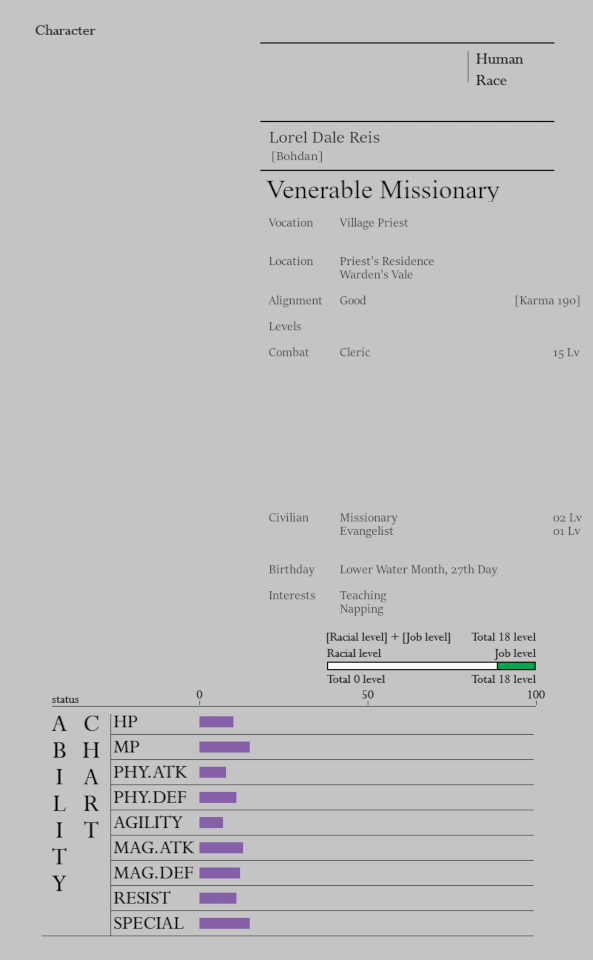
\includegraphics[width=1\linewidth]{images/17LKe7u.png}
    \caption*{Lorel Dale Reis Character Sheet}
\end{figure}

\section*{Character Dossier: Lorel Dale Reis}

Lorel Dale Reis, or Bohdan – as he was known locally to the inhabitants of Warden’s Vale – was born in the southern cities of the Slane Theocracy 119 years before the founding of the Sorcerous Kingdom. The second son of a common warehouse clerk and a seamstress, he was brought up in a meagre household, destined to follow in his father’s footsteps as an apprentice.

 

His fate was changed when a shift occurred in the policies of the Slane Theocracy as its leadership began preparations for the next wave of Players: directing their various institutions to expand recruitment, education and training. Bohdan was swept up as his generation was readied for what may have come. Joining the ranks of the priesthood as an Acolyte, Lorel experienced a curriculum that not only included the Theocracy’s stringent training, but also studied events related to Player waves – notably those of the Eight Greed Kings, the Thirteen Heroes and the Six Great Gods of the Slane Theocracy. The vast majority of this generation never realized what they were being prepared for.

 

Though his tenure as an Acolyte was meant to gird him for those coming times, he ultimately found his calling elsewhere. To the north, the call of a burgeoning Human civilization pulled the young Lorel away from his homeland to answer the growing need for priests and missionaries to both aid the growth of Human realms and spread the faith of the Six Great Gods. At the age of 18, in his search for a place to serve humanity, he encountered Andrei Zahradnik. The intrepid Ranger captured both his admiration and respect, and Lorel would settle in Warden’s Vale, serving the Barony faithfully as its priest for four generations.

 

After receiving news of the Re-Estize's defeat at the Battle of Katze Plains, Bohdan headed the flight of the residents of Warden’s Vale, meaning to lead them to the safety of the Slane Theocracy. He, along with those who followed him, vanished some time later in the wilderness while en route to their destination.
\part{Act 2}

\chapter{Ludmila Zahradnik}

Ludmila’s anxiety mounted as she was led out of the clubhouse and over the swept garden lanes towards the Royal Villa. The waning light of the evening cast a fiery orange glow onto their surroundings as the shadows of the district lengthened over the pristine grounds surrounding the palatial building. Her guide continued to maintain her perfect posture even as she moved ahead: back was held straight and hands arranged primly in front of her. The maid’s hips did not sway, nor did her head bob as her measured gait carried her forward. Even her light adornment – a simple azure bow with a matching sash fixed into a cummerbund – did not infringe upon the image that she projected: that of a perfect and proper attendant.

 

Though she lived in the rough and wild borderlands of the frontier and knew little beyond basic aristocratic conduct, the maid’s composure was such that Ludmila felt compelled to emulate the elements of her own form to match. As she did so, it invariably drew other comparisons between the maid and herself, which in turn fed into her growing anxiety. In figure and form; in grace and manner, Ludmila seemed to fall conspicuously short on every front. She knew that the royal family of Re-Estize practiced a custom which employed young, unmarried noblewomen from prominent families as maids in Valentia Palace, but she imagined that the woman gliding across the cobblestones before her would easily overshadow any of them.

 

It was said that the dignity and skill of a retainer reflected upon that of their master, both on the battlefield and in the court. If such an attendant served the Sorcerer King or even one of his vassals – no, especially if they did – then from what impossible heights of majesty did the Sorcerer King reign? She started to become lightheaded as her sense of self continued to shrink, and after they passed into the entrance of the Royal Villa, she finally felt the need to speak out.

 

“Hold–please, wait!”

 

The maid responded immediately, slowing as she made a seamless turn to face her. Even this simple action seemed almost too graceful to be possible.

 

This isn’t fair! Ludmila cried out despairingly in her mind. She felt unbelievably rustic in the face of her conduct.

 

For a moment, the maid examined her with an unreadable expression before smoothly spreading her skirts in a deep curtsey.

 

“This one goes by the name of Yuri Alpha,” her calm, mellow voice floated up in reply, “my most sincere apologies for not introducing myself earlier, Baroness Zahradnik.”

 

Yuri Alpha rose with a warm smile.

 

“How may I be of service?”

 

That the maid had misinterpreted her mixed expression put a slight crack in her perfect image, but Ludmila’s distraught sensibilities lingered.

 

“I cannot present myself to the Sorcerer King,” she said.

 

The taller woman coolly arched an eyebrow.

 

“Do you mean to say that you are refusing the summons of the Royal Court?”

 

Ludmila’s mouth fell open for a moment before she attempted to explain herself.

 

“I mean to say that I am not in a presentable state,” she said. “The clothes I am wearing are meant for travel on the open roads, my boots are soiled – I need some time to fix my improper appearance.”

 

She had covered quite some distance as she travelled with Momon, and she wasn’t about to present herself to her King in a dusty kirtle and muddy boots. Her hair had been under her scarf for hours and she didn’t even want to know what it had turned into along the way. Her mind went back to Countess Jezne and her reprimand – indeed, she had been the only noble in the room dressed in such a way; clearly unready to attend to official business.

 

Her bags had been taken away from the front desk of the clubhouse by a pair of maids that were instructed to deliver them to her accommodations, so she wasn’t sure where they had disappeared to. Once again, she had been swept along by events and left in a confused and miserable state.

 

“His Majesty is currently attending to business elsewhere,” said Yuri Alpha. “It is the King’s Council that will receive you on his behalf.”

 

The information was surprising, but Ludmila still dug in with the little bit of pride she had left.

 

“As they are acting on his behalf, then I must still conduct myself in the appropriate manner. I will not dishonour House Zahradnik by showing such disrespect to my new sovereign.”

 

Yuri Alpha remained silent, as if to weigh her words. A hand came up as she lightly adjusted the rims of her spectacles. As they shifted, Ludmila realized that there was no reflection of the light coming from the entrance to the Villa – the maid’s eyewear had no lenses.

 

“Very well,” Yuri Alpha said, “but as your presence was requested as soon as reasonable, we cannot spare more than a few minutes to ensure there is nothing untoward.”

 

It did not take long to find a well-furnished drawing room where Ludmila located a mirrored cabinet placed along a wall while Yuri Alpha drew open the drapes. She gingerly removed her scarf, but discovered to her relief that her hair had not become an entirely unruly mess after hours of travel. As she started to slowly comb her fingers through it, a small brush appeared over her shoulder – Yuri Alpha had come to stand behind her.

 

Ludmila received the comb with an expression of gratitude and started to brush her hair as Yuri Alpha worked to remove the bits of her journey that had stuck to her outfit. They worked in silence until Yuri Alpha rose, which prompted Ludmila to return the brush. Checking over herself one last time in the mirror, she felt like she was about to go fetch water from the river rather than attending an official audience with the King. The moist green odours from the woodland trails still clung to her – hopefully she wouldn’t be standing too close to anyone…

 

They returned to the hallway and resumed walking to the council chamber deep within the villa, and Ludmila looked to the grand friezes that lined the walls while she pondered how she should present herself. While the Zahradnik Barony was an independent fief under the Duchy of E-Rantel, Lord Rettenmeier had governed as Royal Provost while holding his position as Mayor of the city. He had a personality that belied his corpulent appearance, and the descriptions of his interactions with Baron Zahradnik – who shared the same straightforward and pragmatic personality – had spoken nothing of the pomp and circumstance that befitted a meeting with a sovereign.

 

Ludmila sighed as she faced forward again. They turned the final corner leading to the audience chamber, and Yuri Alpha led her to a row of seats placed along the wall opposite to the massive Ironwood doors that marked the entrance to their destination.

 

“Please have a seat, Baroness Zahradnik,” Yuri Alpha turned briefly to speak to her, “I shall enter and inform the Council of your arrival.”

 

Ludmila nodded in understanding, then settled herself on the nearest chair. The entire row seemed to be made up of the same low-backed hardwood stools with equally hard wooden seats – it was as if someone was saying don’t get too comfortable to those that waited on their appointments. Having been either on her feet or riding for most of the day, however, the opportunity to rest was welcome.

 

Yuri Alpha closed the council chamber door behind her, and Ludmila looked down the hall both ways before stretching, trying to relieve the tension that had wound up both her mind and body. As she did so, an unfamiliar woman’s voice could be heard in muffled tones through the door. It seemed to be the only voice coming through the door, actually. It droned on for several minutes before pausing, picking up again after a short silence, repeating the cycle over and over again. She imagined this is what she herself might sound like when she relayed instructions, outlined numbers and made recommendations in Warden’s Vale – even her own family looked for ways to escape after being subjected to too much of it at once. Unlike her family, however, she did not think any of the King’s Councilors would come bursting out into the hall in a desperate attempt to flee.

 

After what she thought must have been at least forty minutes, the woman’s voice stopped entirely after slowly losing its momentum over time. Ludmila rose from her seat and stepped nearer to the doors, anticipating her summons. She stood by patiently, ears straining for the approach of someone inside to come out and announce her entrance. The first sound she heard, however, was the rustle of cloth and the sound of vague movement, followed by a lilting, feminine voice that chimed from within.

 

“Well, if that’s all there is, I suppose I should find this Baroness Zahradnik.”

 

After a short pause, Ludmila heard the light tapping of heels slowly approaching the doorway at a deliberate and measured pace. The heavy ironwood doors silently swung inwards to allow a figure to drift out of the chamber and into the hall. Ludmila quickly checked her posture and made ready her greeting but was spared barely a glance; bright, crimson eyes briefly flashing over her from behind an exquisitely crafted fan. The figure turned without missing a step, the hem of her black gown swaying lightly over the polished marble floor as she made her way down the hallway.

 

Ludmila stood, mouth agape, her greeting left unspoken as she was passed by in a flash without a single word. She barely turned her head to observe the woman who had passed her when a wave of murderous ire billowed out from the still-open door. Terror froze her in place until her instincts compelled her legs to send her scurrying down the hall. She dared not turn her head to look into the room as she darted by, instead following after the woman who had long since disappeared around the corner that led out to the main hallway of the building.

 

It was only after the exit of the Royal Villa came into view that Ludmila slowed, struggling to control her panicked breathing. Amidst the wild pounding of her heart, she looked toward where the woman had continued forward – she had paid no mind to Ludmila’s flight down the hallway. Through the clear crystal of the inner doors, she spotted her standing in the vestibule of the building. Two other women had appeared from somewhere to stand beside her. Their sensuous curves were silhouetted by the light of the evening beyond the entrance, ivory figures draped in alabaster cloth.

 

One stepped forward to open the door as the fan in the first woman’s hand snapped shut and disappeared into her sleeve. At the end of the motion, the handle of a parasol appeared over her wrist. Ludmila blinked; the accessory had mysteriously appeared out of thin air without so much as a word or gesture, causing her to wonder if she had lapsed from fatigue after her long journey. The remaining attendant paid no mind to this unexplained phenomena, however: bending at the waist with her arms held out before her. Ignoring the offer of assistance, her mistress left the vestibule, opening her parasol with a smooth motion and bringing it to rest over her right shoulder before proceeding down the lane through the villa gardens.

 

The door whispered softly to a close as the two attendants assumed their places, following behind on either side of their mistress. Ludmila stepped forward to place her hands on the handles of the inner doors, then stopped. As her thoughts freed themselves of the haze of terror, she realized that while events had brought her to this point, she had no idea what she was to do now. The session of the Royal Court had apparently ended, but she was never brought in to present herself. No one had come to retrieve her, and the person that seemed to be looking for her had just walked away without a word. Was she to remain in the Royal Villa until whatever business she was brought in for was concluded? Should she continue following after the lady who had just left? Feeling completely lost, she wished Yuri Alpha or Momon would appear to explain what was going on to her.

 

“I suppose if woodlice become overly large, they cannot creep under doors.”

 

Just as she thought to look for Momon, cold and scornful words prodded her from behind.

 

She turned with a start, finding that Nabe had at some point come into the hallway behind her. She stepped towards the vestibule where Ludmila stood with her right hand still grasping the door, coming to a stop behind her. Long accustomed to her inhuman appearance, Ludmila removed her hand from the door and faced the Adamantite Adventurer. Empty eyes looked upon her from a featureless face, but the beautiful visage superimposed over it wore an expression that mirrored the tone of the words that came before. It occurred to her that this was the first time that Nabe had spoken to her directly, but her desire to clear her own confusion spared her no time to ponder how she had been addressed.

 

“Momon, where–”

 

Ludmila started to ask after Nabe’s partner, but was cut off abruptly.

 

“Momon has left to attend to business elsewhere,” Nabe said. “There is no reason for you to linger here.”

 

A finger tapped impatiently on the Adventurer’s hip. Nabe looked at her expectantly, as if she might conveniently vanish at the end of her sentence.

 

“What about the summons?” Ludmila asked, “The court seemed like it was adjourning…am I to follow the lady that just left, then? It sounded like she was looking for me…”

 

She still did not understand what was going on, so her words simply spilled out in the direction of the Adventurer as she asked weakly for guidance. Nabe succinctly provided an answer; the disinclined tone made it seem more like she was simply trying to get her out of the way.

 

“Lady Shalltear has claimed you in accordance to orders she has previously received from the Sorcerer King,” she said. “You are now hers – the Guardian Overseer has left your matters in Lady Shalltear’s hands.”

 

“Lady Shalltear? The King?”

 

Ludmila felt that the answer left even more questions, but as she parroted the Adventurer’s words, the tapping finger stopped and Nabe’s cold gaze turned into a glare.

 

“Woodlice should not be blocking doorways. Move.”

 

Nabe’s tone did not change, but Ludmila had the feeling that she would be swept out of the villa entrance like some unwelcome insect if she stayed to continue her queries. She turned and opened the doorway, stepping out into the evening air. The sun had crossed below the inner walls of E-Rantel, and the tall lamps of the central district now cast their light over the empty streets. As she walked through the gardens and down the path that led out of the front of the Royal Villa, the clink of metal on stone sounded from behind.

 

Ludmila turned her head to glance over her shoulder, and saw that Nabe was following behind. Passing under another lamp, the glint of light over some polished surface drew her attention to the fact that Nabe was not in the travelling garments that she had seen the Adventurer in earlier in the day. Nabe was dressed in a pitch black dress with some white frills lining its hems, but its many plated segments denied the notion that she might be simply going out to enjoy some part of the city. Ludmila had never seen an mage equipped in such armour before, but she had no doubts that the Adventurer was equipped for combat.

 

“Your armour…did something happen?” Ludmila attempted to start a conversation with the Adventurer.

 

To her surprise, Nabe responded.

 

“The Guardian Overseer has requested that I deal with an issue in the southwest.”

 

Ludmila’s pace slowed somewhat as she thought on Nabe’s words. Did she mean out on the frontier? From what she saw, the way back from Warden’s Vale had very little in the way of anything that suggested internal threats like bandits or roaming monsters. She raised her head from her thoughts as the Adventurer walked past her.

 

“If it’s something on the border…” Ludmila said, “is there anything I can do to aid you? I know the lay of the land around my barony fairly well, as well as the surrounding areas. If there’s some information you would like–”

 

“Lady Albedo has provided me with everything I require,” Nabe curtly cut her off.

 

Veering to the right, the Adventurer stepped onto the path leading to the gazebo where they had arrived earlier in the evening.

 

Ludmila stopped to watch as the mage stepped onto the raised floor of the structure. With Warden’s Vale abandoned, any incursion from the frontier would be met with no resistance, and Adamantite Adventurers were beyond the means of her family to hire. She could do little to repay the favour granted by Lady Albedo – the Guardian Overseer? – but, in her current situation, she could at least express her gratitude.

 

“Thank you for your assistance,” Ludmila bowed her head slightly in Nabe’s direction as the mage made preparations to depart.

 

Nabe turned to look back at her with a strange expression on her human visage. Several seconds passed before her face relaxed a bit.

 

“Lady Shalltear is not one to be kept waiting,” the Adventurer told her. “It is inadvisable to court her displeasure.”

 

With the parting word of caution, Nabe whispered a spell and vanished.
\chapter{Ludmila Zahradnik}

Left alone with her thoughts in the empty garden, Ludmila scanned the surrounding district. Though not much time had passed, she could not spot the figure of Lady Shalltear or her attendants anywhere. With little to achieve by standing around, she searched through the areas nearest to the main street, her head turning back and forth as she walked. Eventually, she stood in front of an imposing gatehouse that marked where the main promenade led south into the rest of the city and, with a tired sigh, she stepped across its threshold to take a look beyond the wall.

 

The layout of E-Rantel was suited to its nature as a fortress city. Though protected by three massive curtain walls, the arrangement of the streets was such that any invaders that did make it into the walls encountered a somewhat confusing urban labyrinth. There were no strongholds that were designed to resist hostile forces in each section following a breach, but there were also no clear and direct paths to anywhere important. Even the main thoroughfares followed winding routes through the buildings of the city on their way to the next set of gates. The nature of certain industrial areas within the main section of the city could be identified by sight and smell, but there were no clear written markings or directions to assist outsiders with navigation within or between the various parts of the city. To those unfamiliar with its ways, most of the city’s layout would appear a random mix of shophouses, apartments, inns, warehouses and all manner of institutions such as temples, guilds and artistic venues.

 

Outsiders themselves, her family would hire a wagon that would take them to the various warehouses where they would sell their goods to wholesalers, who would in turn make their living by reselling their inventory as the markets demanded. She recalled her younger self staring out from their hard seats as they wound their way through the veritable maze of streets, buildings and plazas. Even now, as her gaze followed the main road down the slope from the gate, she was under no illusion that she wouldn’t quickly become lost the further she went from the Central District’s entrance.

 

Lady Shalltear and her attendants should have stood distinct from any of the city folk, so she had thought to inquire after their passing with any citizens she could find nearby. However, it turned out that the streets beyond the inner walls were just as empty as those within them. Streetlamps, less ornate than those in the Central District, shone with the same intensity nonetheless: brightening the empty thoroughfares of the city which lay in still and eerie silence. E-Rantel was a major trading hub as well as a staging ground for mercenaries and Adventurers that worked jobs maintaining the nearby Katze Plains, providing escort to merchants and keeping the highways and roads of the surrounding countryside clear of threats. Even with the sudden and unexpected annexation, this work did not conveniently wait for anyone and the city should have at least had a certain amount of life in the streets. It was an odd sight that she would have normally given more thought towards, had her own business not been so pressing.

 

“Where could Lady Shalltear have gone?”

 

Frustration caused her to finally voice her thoughts aloud into the evening air. Without any leads to go by, she decided to turn back and see if there was any way that the administrative offices in the central district could help her locate the mysterious woman.

 

The groan of metal coming from the direction of the gate caused her to slow mid-turn. Where the gate behind her should have come into her field of view, instead was a murky reflection of herself looking back at her. She faced a wall of dark, polished metal twice her size, gleaming in the twilight.

 

The sound continued as the wall of metal shifted slightly. A movement out of the corner of her eye caught her attention – an arm covered in vambraces of similar material, draped in a tattered sleeve, was stretched out from behind what she now realized was a massive tower shield. The arm ended in a wicked gauntlet curled into a fist, and a single clawed finger protruded from it. As her gaze followed down the arm and eventually in the direction indicated by the finger, she realized that it was probably the answer to the question she had voiced to no one in particular.

 

From her vantage below, she could only see the crest of a shining helm behind the top of the tower shield. The tall guard made no further moves and the cloak of its purple robe fluttered in the evening breeze, making a sound similar to that of a large banner. After standing awkwardly for a moment, Ludmila silently nodded her head in towards the shield in thanks before heading in the direction indicated.

 

Assuming a brisk pace, it wasn’t long before she spotted Lady Shalltear’s dark parasol. The pale figures of her attendants could be seen still flanking her as she strolled off casually barely two blocks ahead. It turned out that she had actually not gone far at all, but the erratic layout of E-Rantel was simply obscuring her line of sight. Breathing a sigh of relief, she slowed her pace and mulled over how to present herself and the issues that faced her family’s demesne.

 

As she calmed down and ordered her thoughts, the monumental task that lay before Ludmila formed a growing list of problems in her head. She maintained a vague sense of Lady Shalltear a few dozen paces out in front of her, but for the most part she had focused herself inwards in order to sort everything out.

 

The most pressing issue was that Warden’s Vale currently had a population of one: herself. Without labour, there would be no production, no revenues; stagnancy and decay would soon follow. The normal means by which rural territories secured immigrants – through petitioning the city administration or checking with the temples for hopeful settlers, refugees and the homeless – would not work for frontier fiefs. One could not simply be a Farmer or any other singular civilian profession: if the population was not accustomed to life bordering the wilderness and incapable of holding their own against the threats that lay around them, they would not survive for very long. The weak would simply become food for predators, and becoming known as a place to find easy meals only invited more unwanted guests.

 

Though the Sorcerous Kingdom – according to Countess Jezne – had a standing army, Ludmila was not certain if they possessed the ability to uphold the borders and maintain constant readiness against potential attacks from the wilderness. All it would take was an hour or two and the entire village could be ransacked by a tribe of Demihumans if it lacked ready defenders. Warden’s Vale had established itself as an entrenched Human territory in the eyes of their savage neighbors, but there only needed to be a curious scout or a desperate hunter to find that the village was now open to invasion. The thought did not sit well with her at all, especially considering that Nabe had already departed to deal with some sort of issue in the area, and it was something she wanted to remedy as quickly as possible.

 

The other problems revolved around logistics, such as building a new vessel to transport the village’s goods and refurbishing old infrastructure, as well as making sure all of her legal affairs were in order. She also needed to ensure that her understanding of the law was still in line with that of the new administration’s. In addition, she needed to figure out where her village’s goods disappeared to and hire a wagon to transport and sell them…but all these things would not avail her any if she did not resolve the first problem.

 

The only recourse that came immediately to Ludmila’s mind was the courtier that she had ultimately followed after. Her proud bearing and lavish attire gave off the air of one accustomed to high society and, according to Nabe, she had a connection to the Sorcerer King. Ludmila was not sure if she was actually a noble, but at the least she had risen to a position where her value warranted her attendance in the Royal Court. If she was a powerful noble, the resources she might be willing to bring to bear would make all of Ludmila’s worries seem needless in the end.

 

Resolving herself, Ludmila picked up her pace to catch up with the small procession ahead. Her lonely shadows projecting onto the buildings lining the street made her keenly aware of how much the city had changed from her past memories. The wooden-framed structures with their walls of wattle and daub were sometimes five or six stories tall and even a small city block could house several times the population of her entire fief. This normally meant that street life should be boisterous as labourers parted with their wages in the evening, so the contrast with the reality she was currently experiencing created a dissonant sensation.

 

Every door was shut; every window shuttered. The occasional wisps of smoke she could see rising from chimneys indicated that they were indeed occupied, and that the residents were burning fuel to keep warm in the chill of early spring. She could not make much sense of it. Ludmila understood that the events of Katze were certainly terrifying, but E-Rantel itself did not look like it had been damaged. The streets were unnaturally clean and there was no sign of any looting or arson that one might think would come hand in hand with a violent siege and occupation. For all of its changes, the city still needed to run. Food, fuel and rent would need to be paid for somehow, and the various organizations and businesses in the city still needed to operate to keep trade and production flowing.

 

As she advanced, she saw that Lady Shalltear and her attendants had crossed into a large plaza, passing one of the many militia posts placed around the city. There was a sentry posted that was vaguely similar in appearance to the one that had given her directions earlier: it had the same dark armour, but with veins of bright crimson running through it and it didn’t appear to have the same cloak or robe. Rather than a bright, shining helm, this sentry wore one that was as dark as the rest of its armour. The armour itself had dozens of wicked spikes protruding from it which made her curious about the rest of its appearance but, much like the previous guard, she could not see over the massive wall of dark metal that was its tower shield to take a look at the person behind.

 

The sentinel stood motionless as she crossed in front of it, and the flutter of leathery wings from above drew her attention. Perched on the lamppost that came out over the street from the militia post, an Imp peered down at her with shining eyes. The bright light from the enchanted lamp that hung from the post was reflected off of its copper skin and cast a large shadow of the winged creature on the tall building looming over the guardhouse. She continued to look up at it as she passed under the lamp, and it grinned down in return like some sort of sinister gargoyle come to life. Ludmila had only seen and heard of them from books and the tales of performers, yet their descriptions had matched so closely that she was instantly able to identify it. The creature itself was rather small, so she felt more wary than threatened at its appearance.

 

Ludmila pondered her relatively calm reaction at the reportedly evil being, and her head turned back down to look into the window where the post’s officer usually presided from. With how quiet the city was, she thought it may have not warranted being manned, but a ragged figure stirring inside proved otherwise. A desiccated hand appeared at the counter, and the figure leaned forward into clear view. She followed the flowing black fabric of its robes until her eyes came to a stop at its face. Two points of angry crimson light flared back at her – it was a dead man’s face, weathered by the passing of untold ages. Its flesh had dried and pulled back his thin lips in a ghastly sneer as he stared down at her from the guardhouse window.

 

She let out a startled cry as she immediately fell away, tumbling onto the flagstones of the pavement. She scrambled back to her feet and fled into the plaza. Rows of stands and benches filled the space – it was a place which would usually have hundreds of merchants displaying their wares and many times the number of citizens, travellers and other folk perusing the vast selection of goods. But like the street that she had dashed out of, it was silent and empty, the evening wind blowing across what should have been a vibrant centre of city life with a lonely moan. Neither sound nor movement could be heard following, but she dared not turn to look over her shoulder as she bolted forward.

 

With the shift in how she profiled her surroundings, she began to notice other things as well. The Undead she had encountered at the militia post was not the only one. Several similar figures in black robes flew over the plaza, vanishing over the rooftops and out of sight while others appeared shortly after, heading in different directions. In each corner of the plaza, there was a similar guardhouse and the one that she was quickly closing in on seemed to have the same arrangement: a tall, dark sentinel with a tower shield and an Imp perched on its lamppost. Nothing had reacted to her panic, but she made a wide circle around the guardhouse as she followed after Lady Shalltear and her attendants, who seemed to be entirely unruffled as they had passed. Slightly incensed at the sight and the fact that she seemed to be the only person reacting to everything, Ludmila brushed off her skirts and took a closer look at the street that they followed. As she continued to examine her surroundings, she thought back to her encounter at the first militia post, recalling every detail.

 

Several minutes passed before their winding route led to another small plaza. She walked directly up to the militia post ahead and steeled herself. If a citizen had seen her, she thought that they might have shouted out in warning or terror. Perhaps they would have marveled at her foolishness and awaited the inevitable, gruesome result. But when she stepped directly in front of the sentinel and its grimly gleaming tower shield, Ludmila did not sense that she had any spectators.

 

As she reviewed her journey through the streets of the city, she reoriented her perception. Even with the Undead present, E-Rantel was undamaged and of the slaughter of its citizens, there was no sign. The sentinels had not reacted to her presence and nothing had chased her when she fled in panic. The only time she had gotten any sort of response was when she received directions from the guard at the gatehouse. She looked up past her reflection in the shield to the crest of the helmet peeking above it. The Imp sitting on the lamppost was looking down at her, but she decidedly ignored its grinning leer. Poking her head around the shield, she took a close look at the sentinel from the side.

 

Eyes that glowed with angry crimson light glared back down at her, but the sentinel did not stir beyond its notice. As Ludmila registered the features behind the open face of its helm, she had no doubt that this sentinel was Undead. She suspected that every one of the dark, armoured warriors she had walked by were also Undead, but their behaviour was unlike any Undead she had seen before.

 

Occasionally, the wilderness tribes in the upper reaches would have conflicts between themselves, and the dead bodies resulting from their battles would be washed downstream. These corpses would occasionally result in Undead like Skeletons and Zombies that pulled themselves out of the water, drawn to the abundant life in Warden’s Vale. They would immediately chase after the hundreds of geese wandering around the marshy floodplain, which created an endless, annoying racket until a handful of villagers showed up to put an end to it.

 

Since she couldn’t even sense how strong they actually were, these Undead were far more powerful than the Skeletons and Zombies that occasionally popped up in the barony…but they seemed to care nothing for the living beyond observing them. While they did not exactly seem to be inclined to interact with her like Human militia might, they were sentries all the same. Ludmila turned and stepped away from the sentinel, walking past the guardhouse. Looking into the window, she saw there was the same type of Undead that had startled her witless before staring back at her. She held its gaze as she passed the guardhouse, satisfied with the result.

 

While it appeared that death stood in the streets and flew in the skies overhead, the truth was that the city of E-Rantel had been laid siege to by the spectre of their own fear.

 

Ludmila continued on her way down the street where Lady Shalltear had gone, no longer paying any mind to the Undead standing watch over the city.

 

Duty cared not for fear, and time awaited no one.
\chapter{Ludmila Zahradnik}

By the time Ludmila caught up with Lady Shalltear again, they were crossing another, smaller plaza on the western side of the city. The evening light cast itself between the spaces in the streets and buildings, painting their path with its fading glow. The dark folds of Lady Shalltear’s gown swirled in contrast to the pale white figures of her attendants; its luxuriously rich fabric seemed to eagerly devour what remained of the day. Her parasol still lay over her shoulder, twirling idly on occasion and obscuring Ludmila’s view.

 

Though she roughly knew what she needed, Ludmila still struggled to find the appropriate words to convey her plight to Lady Shalltear. After settling herself with the presence of the Undead, other worries arose: worries that if she slighted her in some small way, even unknowingly, she would doom her demesne to ruin. Thus, she continued to follow silently after her as she worked up what little she knew of dealing with high nobility and deciding what forms of etiquette would be appropriate to observe.

 

She followed them out of the plaza, along the large road as it meandered through the buildings. It continued to feel unnaturally empty; no one looked out of the shuttered buildings on either side on the road to watch their procession. At each intersection, the dark sentinels stood tall beneath the streetlamps, in silent challenge to any opposition.

 

As far as they had travelled, Ludmila wondered if their journey would simply continue in its winding circuit around the rest of the city and have them arrive at the northern entrance to the central district. She found herself drawing closer to the trio ahead of her as she thought of their journey continuing past that, entering the less reputable and poverty stricken areas of the city, before noticing that the group ahead of her had slowed their pace. Looking to the gatehouse at the wall that set the poorest sections of E-Rantel apart from the rest, she saw two more of the same dark sentinels standing on either side of a closed gate. A heavy wooden bar lay across it; she realized that the pauper’s quarter had been closed off. No signs of activity could be heard over the wall and Ludmila wondered why it was so, and if the residents still remained within.

 

Her question would remain unanswered as the entourage turned a few blocks before the gate, into an alley between a pair of prominent buildings: a large inn that appeared to be meant for all manner of guests with a tavern on its ground floor, and a warehouse belonging to the Merchant Guild on the other. Unlike the main streets, the smaller lanes and alleys of the city were not paved and had damp sections left over from the wet winter season of the lowlands. The stretch nearest to the street was a loading area for the warehouse and many wooden planks of varying lengths were laid over places where wagon wheels had worn muddy ruts into the alley. Looking into several of the open loading bays as they passed, she saw that the building appeared to have been vacated: nothing but scraps of paper and a few discarded crates strewn about the warehouse floor. The inn opposite to it was shuttered and locked away like many of the other buildings in the city that she had seen along the way.

 

As they moved beyond the warehouse, the height of the surrounding buildings grew shorter, but the alley tapered to a width that could only accommodate pedestrians. In front, Lady Shalltear and her attendants walked single file: the alabaster-clad women coming before and after their mistress. Ludmila slipped in behind them, not wanting to stray too far in the lonely passage. The lane was no longer as straight as it had been nearer to the main street and angled one way or another as they advanced. Their path now seemed more like a narrow canyon than a city alley; the soil under their feet remaining damp and muddy with the pittance of sunlight it probably saw in a day.

 

She focused on her footing as they made their way down the alley, stepping around puddles and potholes that intermittently appeared along the way. A short while later, Ludmila felt wisps of the cold spring breeze filtering down between the crowded buildings. Faint hints of woodsmoke were carried along with it, and she raised her gaze to look far ahead at the first signs of life she had seen in the capital since her brief visit to the Royal Villa.

 

Shadows cast by the flickering orange flames of an unseen fire danced on the alley wall. Any details were still too distant to make out, but the smoke-tinged air carried with it the distinct smells of Human habitation: the aroma of food being cooked and the odours of sweat and worn fabrics. As she approached, the surroundings grew brighter and the faint murmur of voices carried through the haze of cook fires: over which hung large, cast-iron cauldrons. Overhead, she noted open windows where people of various ages could occasionally be seen inside. Many curiously looked down at the small group that had come in from the main streets.

 

It was a short distance before the alley opened up into a small courtyard nestled deep within the packed buildings. Tall braziers had been placed at the corners of a crudely cobbled square and several men and women stood about them, speaking amongst themselves in low tones. Despite signs of having been cleaned up recently, there was no hiding the age of the buildings that surrounded the open space. Yellow and brown watermarks stained the walls. Patches of whitewash and old clay plaster could be seen all along them. This tiny pocket deep in the bowels of the city seemed to have been forgotten by time: a throwback to an age when the city was still young; the streets and buildings less grandiose. Even the materials used to construct the buildings and the layout of the yard seemed fashioned in an entirely different style to the main thoroughfares of the cosmopolitan city that they had left behind along with its paved roads. Perhaps only those that lived nearby even realized that the hidden plaza existed.

 

A middle-aged man bearing an unmarked load over his shoulder crossed in front of them, bending slightly in respect to the group as he passed by. His gaze lingered on the women but his pace did not slow as he vanished into the narrow alley to wherever his destination lay. Going by the reaction of the people who noticed them, it was not the first time they had seen Lady Shalltear and her attendants in this secluded little pocket of the city which was well out of sight and away from the Undead sentinels.

 

The way the people carried themselves and interacted amongst one another marked them plainly as common folk, but they did not have the fresh appearance of villagers in more rural areas like Warden’s Vale. Though they appeared to have done what they could to maintain their appearance, many had worn clothing marked with the grime, soot and sweat of city life. These were the citizens that worked in the alleys and buildings behind the pristine storefronts, guild offices and warehouses of E-Rantel – the hands and feet and backs supporting the city’s twin pillars of commerce and industry.

 

As Lady Shalltear made her way towards the centre of the plaza, Ludmila looked for a place where she could quietly observe its people without getting in the way. Two women standing under one brazier took note of their passage and after a quick exchange, one of them hurried off into the short doorway of a nearby building. The remaining woman turned to approach one of Lady Shalltear’s attendants. Standing in an unoccupied space behind the group, Ludmila could not make out what the woman was saying as she bowed her head, but the low, plaintive tone made it seem like a petition of some sort. The attendant remained silent and made no motions as she heard the woman out.

 

With the sound of the woman’s voice in the background, Lady Shalltear and her remaining attendant made their way to a small pile of crates where another attendant with a slightly different hairstyle stood with a clipboard in hand. Their mistress stopped and turned to survey the surroundings, looking back towards the way they had come and the small groups of people going about their evening. The other attendant had moved forward to meet the woman standing at the crates, who began to speak at length with the clipboard held in front of her, gesturing at intervals with some sort of pen in her other hand. The mannerisms of a warehouse clerk were at odds with her fine appearance, and Ludmila observed bemusedly from the side as the two conferred quietly between themselves.

 

The return of the first attendant caused Ludmila to turn her attention back to where Lady Shalltear stood near the middle of the yard. She continued to stand with her back turned to her as she listened to what the attendant had to say. Four long shadows extended from her figure, cast by the braziers in each corner, dancing across the ground as the fires flickered and crackled around her. The parasol had disappeared somewhere and the long fan had returned to her left hand. After receiving a slight nod from her mistress, the attendant in turn looked to where the petitioner stood and motioned for her to approach.

 

The woman walked to the building where her companion now stood supporting a third girl in the doorway, and together they helped her come forward to the lady clad in shadowed silks awaiting in the middle of the courtyard. As the trio came fully into view, recognition caused a memory from a year past to jump out at her: a startled and pained yelp from one of her brothers as their father pulled his ear sharply to turn his gaze away from some gaudily dressed and painted women standing at a street corner. It was evening as they were returning to the central district, on an empty wagon through the streets of the city, and her father – who was preoccupied with scolding his sons – did not notice that his daughter was examining their appearance as well. The two women supporting the third, though not nearly as brightly dressed as those from her memory, were most likely prostitutes.

 

Slowly shuffling forward as they supported the girl between them, the three women came before Lady Shalltear, gazes cast downwards. After they helped the girl kneel before her, the first two respectfully backed away, bowing multiple times before stopping to stand quietly at the edge of the plaza. Wrapped in a short, worn blanket, the woman kneeling on the ground shivered in the chill of the early spring evening. She had a thin, ragged appearance and her skin was marred by cuts and bruises. There was a dark splotch where she had received an injury to her head over her left temple, and a deep cut caked her blonde hair with dried blood and glistened slightly as it continued to ooze. Her light blue eyes seemed to focus and unfocus unsteadily as she looked down at the hem of Lady Shalltear’s gown. The girl did not seem quite there. Ludmila looked at the gash over the side of the woman’s head again and decided she must have suffered some other, unseen injury from being struck.

 

The arrival of the injured woman had drawn the notice of several passers-by, who had been alarmed at her bloodied appearance as she was carefully led to the tiny plaza. As they stood to watch, others slowed down and stopped to see what was going on. Silence grew over the courtyard, and eventually only the occasional crackling of the braziers punctuated the still night air. Out of the corners of her vision, Ludmila could see the people scattered around the rough, cobblestoned yard watching the two figures in the centre of the plaza. The sudden quiet led to residents appearing in the windows overhead, looking down for the source of the uncharacteristic stillness in the air. Lady Shalltear stood silently at the centre of attention, as if waiting for the expectant energy in the air to rise further. Then, without word or flamboyant action, she stretched her hand out to the woman kneeling before her.

 

As she reached forward, Ludmila’s eyes grew wide as she noticed for the first time what had been obscured from her vision as she followed Lady Shalltear through the city. Where a slim, delicate arm with beautiful porcelain skin glowed in the firelight also appeared pallid flesh stretched over a sinewy appendage. It extended far longer than that of a normal person’s, ending in a hand with elongated fingers tipped in what were far too long and sharp to be Human nails. As she cupped her chin, the woman showed no reaction to this monstrous sight and Ludmila understood that it was something that she alone was perceiving through her Talent.

 

Ludmila’s mind whirled, trying to understand what she was seeing. Lady Shalltear tipped the woman’s chin upwards to face her fully and, after a moment, her clear, feminine voice could be heard across the plaza.

 

“「Regenerate」.”

 

A bright, magical glow briefly pulsed over the woman and the bruises visible on her face and body faded away without a trace. The gash over her temple closed as the spell mended the cuts on her skin. The girl blinked as the pain that must have accompanied her injuries slowly subsided. Her jaw worked as if to speak, but the fingers grasping her chin maintained their firm hold.

 

Lady Shalltear’s voice sounded again.

 

“「Remove Disease」.”

 

A second, dimmer, glow issued over the woman – this time she froze in place, eyes looking up at Lady Shalltear. In the silence that followed, a tear rolled down one of the woman’s cheeks, then the other. All at once, she collapsed to the ground, sobbing quietly. By the third shuddering breath, her quiet, wracking sobs had grown to a wail that filled the night air. The woman tightly grasped the hem of Lady Shalltear's dress, pouring into it a life of desperation and anxiety; of fear and shame. At the edge of the plaza, the two women that had brought their companion forward were wiping tears away as well.

 

Though the weeping woman clinging to her dress was at least half again Lady Shalltear’s height, her small figure did not budge. Indeed, it seemed that she paid the weeping woman at her feet no mind at all, instead intent on once again observing her surroundings.
\chapter{Ludmila Zahradnik}

The events unfolding in the small back alley square had, by then, drawn a crowd of people. Some had come from the surrounding alleys, while many others occupied the windows looking down into the dimly lit area. They looked on in silence as the heartfelt sobs of the woman continued, seemingly unwilling to disturb the scene playing out before them.

 

From her place behind the impromptu stage, Ludmila silently digested the events leading up to the scene before her. Until that moment, she was unable to make very little sense of their course so far. The reason why this highborn lady, who had a direct connection to the King, would walk halfway around the city to some forgotten back alley on the border of the slums had been a complete mystery.

 

The revelation that Lady Shalltear was a divine caster shed some light on the questions that had continued to rise in Ludmila’s mind. It would not be uncharacteristic for a priest to come and minister to the people. Were her attendants clad in their fine, alabaster garments Acolytes? Their uniform appearance lent credence to this thought. The light, almost sheer cloth of her attendants’ garb could perhaps be found in much warmer regions of the world. The black gown and bolero of Lady Shalltear with its silver and carmine highlights, however, did not match the vestments of any faith she had ever encountered or read of.

 

What manner of priest is she? She wondered to herself.

 

“Cleric.”

 

Lady Shalltear’s voice snapped Ludmila out of her thoughts and she focused her attention on her.

 

“Cleric,” the correction came again, “not Priest.”

 

It was then that she realized that, at some point, she had voiced her thoughts aloud. Though the words had caused her to go silent once again, she couldn't hide the dubious expression that painted her face. Clerics were a part of the priesthood of every religion she knew of. Though they were often trained and specialized for the battlefield, they usually did not mind being called priests. Looking at the back of the slight figure before her, she could not imagine a woman so much smaller than herself standing at the forefront of pitched combat: bolstering her allies and delivering divine wrath upon her enemies.

 

“But surely you are here to minister to the people?” Ludmila asked.

 

This was the first time since they had encountered one another that Ludmila had Lady Shalltear’s attention, so she quickly brushed aside her doubts at the previous statement to press her with questions. As Bohdan had tended to the needs of her village, so too did the priesthoods of larger towns and cities serve their own populations. They gave spiritual guidance, performed charity and though they legally held no political power in Re-Estize, the Temples had a degree of cultural influence and certain rights concerning the use of divine magic.

 

She voiced her query, and Lady Shalltear's posture stiffened momentarily. A short silence ensued. The fan, which she had been waving lazily in front of her face, snapped shut. She turned smoothly with her head tilted slightly, the silken folds of her dress swirling around her.

 

Though Ludmila had mentally braced herself after seeing the Cleric laying hands on the battered and sick prostitute, she felt herself take in a sharp breath as what she now saw rooted her feet to the ground.

 

As with Nabe of Darkness, Lady Shalltear had two appearances.

 

The first was that of a peerless beauty – far beyond that of Nabe – something that Ludmila would not have believed possible were she not witnessing it herself. The Cleric’s luxurious silver hair had been tied up in an off-centre ponytail that spilled down the length of her back. Long, lazy ringlets fell about a delicate face of perfect frame; clear and bright crimson eyes turned up towards her beneath long, silver lashes. In vibrant contrast to pale skin reminiscent of a porcelain doll, her cheeks were flush with life while small, soft lips parted with the hint of an alluring smile.

 

It was a bewitching appearance that anyone would fall to; any feelings of jealousy or envy swept aside by adulation and longing. Wealth and power beyond all reason would be squandered to obtain even a moment of her favour. She was possessed of a legendary beauty that could topple nations and spark wars that set the world aflame, and the world would gladly become ashes for her sake. But even as Ludmila stood entranced by this vision, her Talent made her aware of a second, horrifying appearance that lurked beneath the first.

 

Like the arm she had seen previously, pallid flesh was stretched over a face that invoked a dark and primal fear from deep within her. Her mouth, parted in a ghastly smile, was impossibly wide with pale lips stretched thinly around it. All around the inside of her mouth lay row upon row of wickedly curved, needle-sharp teeth, much like the lampreys that would occasionally be found latched to sides of fish caught from the river. A long red tongue writhed sinuously within, running over the carpet of teeth like a fleshy rasp. Glowing crimson eyes shone from within their dark hollows, and Ludmila felt like nothing more than helpless prey. Even the lustrous silver strands that framed her face seemed about to move on their own.

 

As Ludmila stood transfixed by what she saw, Lady Shalltear seemed to be gauging her reaction. The corner of Lady Shalltear's mouth twitched, and when it seemed that nothing more would be forthcoming from the girl standing rigid before her, she straightened from her coy posture to speak.

 

“It is the Will of Ainz Ooal Gown, the Sorcerer King, that His domain stands as a beacon of prosperity and harmony for all the world to see.”

 

Lady Shalltear's answer was clearly not only for Ludmila and her soft, lilting voice chimed lightly across the square.

 

“By the grace of His Majesty, you are afforded protection as His citizens.”

 

The arm holding the closed fan swept out over the onlookers surrounding the square as she turned away from Ludmila with a grand gesture. Her feminine figure swayed seductively in the light of the braziers as she made her way back to the centre of the plaza. By this point Ludmila could see a throng of people gathered in their surroundings – even the rooftops had people looking down from them.

 

Lady Shalltear’s pace slowed as she came back to stand near the stacked crates again. The healed prostitute had collected herself and knelt with her companions. The Cleric’s gaze surveyed the surroundings before finally coming to rest on the wooden containers before her. Following that gaze, Ludmila saw that a meagre-looking plant had been laid on the corner of one of the boxes. With small flowers of white and yellow, she recognized it as one which commonly grew out of the cracks in the pavement and masonry of the city.

 

Producing a silken handkerchief, Lady Shalltear gently picked up the flower, placing it on the cloth to be folded within. Then, while holding the humble tribute in her left hand, she raised her right.

 

“「Gate」.”

 

A hole opened in the air behind where the boxes lay – it was similar to the one that had appeared in the warehouse in Warden’s Vale. Wide enough for several grown men to fit shoulder to shoulder and just as high, it hovered silently in inky darkness. The Acolyte with the pen and clipboard came to stand before Lady Shalltear.

 

“Pandora’s Actor will know what to do with this,” the Cleric said as she handed the wrapped flower over to her attendant, who had her palms held out to receive it.

 

Lady Shalltear’s hand motioned lazily at the crates in a dismissive gesture.

 

“Return these.”

 

As she turned away, another attendant came to pick up one of the crates. The hollow sound it made as it bumped against the others upon leaving the ground suggested that it was empty. Falling in line with the other Acolyte with the clipboard, they stepped forward into the hole in the air and disappeared.

 

After a moment, the Acolytes reappeared with identical crates, but they made a more solid noise as they were set down in place of the ones that had been carried away. Back and forth the attendants went, not seeming to tire or mind their burden. As the crowd looked on, the attendants eventually refilled the space formerly occupied by the empty crates, neatly arranging them behind Lady Shalltear.

 

“It is the Will of His Majesty that His people shall not want for shelter or provision,” the end of Lady Shalltear's sentence was punctuated with a thump as the last of the crates settled on the ground behind her. “It is His Will that His people are provided with the security and stability to thrive – regardless of their ability, occupation or station.”

 

As Lady Shalltear once again wove around the plaza, her swaying movements and graceful steps seemed almost a dance – more suited to the polished floors of a palace court than the dirt and puddles of the alley. The rich silks of her black ballroom gown swept over the ground and the sweet sound of her voice filled the square; those watching stood transfixed by the vision made manifest before them. It was as if they had found themselves transported into a song of legend and they were witnessing a noble of the highest calibre. Their cramped and dirty alley had been transformed into the grand courts of some far-flung empire, where the lady before them was delivering not a message to the riffraff of a city conquered, but a proclamation to the heads of great houses and rulers sitting on their thrones. In one hand she held healing and salvation; in the other she offered peace, prosperity and the hope for a greater future.

 

As she spoke, the attendants had all returned and opened the newly-arrived crates. They revealed food – staples, vegetables and cuts of meat. Others contained bolts of flax and linen, balls of wool yarn and spools of plain thread. Coal and charcoal could be seen filling others still; as well as logs of wood and kindling. A great plentitude of life's necessities were arrayed behind Lady Shalltear as she continued to speak, adding a simple to understand weight to her words.

 

“Those who strive to serve under His rule shall be rewarded in equal measure,” Lady Shalltear rested her hand on the shoulder of the woman she had tended to. “Those that would dare to bring harm to what is His shall be granted no quarter.”

 

She beckoned for an Acolyte to come forward with her free hand. Immediately, one of the gorgeous women clad in alabaster silks stepped before her and deeply bowed.

 

“The one that did this,” Lady Shalltear's voice could be heard clearly across the square as she issued instructions. “Find him, and bring him here.”

 

The woman raised her head, and Ludmila thought she saw a predatory gleam in her dark eyes before she turned away, walking straight towards the edge of the crowd on the opposite side of the square. It took a moment for the bystanders to realize that the last words they heard had been an order, but upon this realization a disturbance arose from the direction the woman was walking towards. The crowd turned their heads. A small opening formed in the wall of people: revealing a tall, lanky man with the appearance of a common labourer. He had already taken several steps, trying to shove through the crowd, but it was too late.

 

“「Hold Species」.”

 

The man froze completely mid-step, magically paralyzed by Lady Shalltear’s spell, his arms held out in front of him as he was trying to push his way through the wall of people in the way. Those around him did not even have enough time to register what had happened as the Acolyte scooped him up entirely, carrying the man like a hollow wooden mannequin back to her mistress with no more visible effort than she had shown when she delivered the filled crates.

 

Lady Shalltear nodded as she opened a new Gate. The man was still frozen as he was carried off to some unknown fate.

 

The spellbound feeling over the crowd had partially broken due the commotion, but the Cleric’s declaration still echoed in their minds. Lady Shalltear had rejected the notion that she was a priest, but what had transpired delivered a message more powerful than any sermon Ludmila had ever attended. As she looked around the plaza at the faces in the crowd, all those present had clearly been moved by her words.

 

No...rather than moved, something had taken root. Though Lady Shalltear’s unveiled appearance had tempered Ludmila’s reception somewhat in her own eyes, she still felt the lingering appeal of her words. A colder, more calculating part of her mind reared up in alarm – an ember had been instilled in the hearts of the people here, and from deep in the lowly alleys of E-Rantel, it would spread and perhaps set all its citizens aflame with the evening’s message. It was something many a noble both sought and feared at the same time, something that could become extraordinarily dangerous if it flew out of control.

 

As she watched the people slowly disperse, the attendants had taken up positions in the middle of the plaza, distributing the supplies to the queues that had formed after their mistress had retired from the stage. Charity was also a component of various faiths, but the sheer abundance before her would have beggared even the largest of city temples before long. As Ludmila watched them work, she felt a presence brush up near her.

 

“Baroness Zahradnik.”

 

Ludmila looked down at the familiar voice and her body jumped – most of what appeared below her was a yawning pit of needle-sharp teeth. She was only thankful that she didn’t cry out as well. Lady Shalltear’s slight stature certainly allowed her to move about without being noticed, if she wasn’t purposely drawing attention to herself. Ludmila had a great many things to ask of her, but everything she had thought of seemed to want to come out at the same time, resulting in her mouth opening wordlessly and not much else.

 

The Cleric in the black gown seemed amused by her reaction, and wrapped a hand lightly around Ludmila’s elbow.

 

“Let us speak privately elsewhere.”
\chapter{Ludmila Zahradnik}

The pair appeared at the same gazebo that Ludmila had arrived in alongside Momon and Nabe earlier that day. Night had fully fallen over E-Rantel, and the cool air was refreshing after being in the crowded atmosphere of the smoky alley plaza. The wide open space under the clear night sky had a relaxing effect on Ludmila as she stepped off the platform behind Lady Shalltear, who had let go of her arm after they had arrived.

 

“This gazebo appears to be quite popular,” Ludmila said casually while stretching.

 

As the words left her mouth, she realized the sort of sloppy appearance she was putting on – not to mention speaking out of turn with a member of the Royal Court. Her heart sunk as she brought a hand to her mouth at her own rude behaviour. All of her efforts to organize proper protocol her mind seemed to have been for naught.

 

“Hm? Ah, that place is the only spot where teleportation isn’t prevented here,” Lady Shalltear peered around the grounds as she responded to Ludmila’s words, not even bothering to turn around before speaking.

 

Ludmila blinked several times upon hearing this. While she had not even known of the existence of teleportation magic before today – never mind that it could be restricted – it didn’t seem like such a good idea to reveal security measures openly in public. Perhaps it wasn’t as important as she felt it was; Lady Shalltear’s voice had lost its formal tone, leaving only her light, lilting voice that seemed not too much different from a young woman around her own age. Ludmila wondered if it meant that she herself could relax and put formalities aside…or perhaps Lady Shalltear was graciously covering for Ludmila’s breach in protocol.

 

Deciding that it would be for the best to not to press her luck, Ludmila remained silent as she followed behind her, resolving her self once again to demonstrate the proper decorum. Lady Shalltear’s attendants had been left behind to distribute supplies to the crowd of people in the plaza, so they walked alone together through the empty streets of the central district. Several of the guest houses they passed had dim lighting that filtered through their windows, so it seemed that the nobles’ meeting had adjourned – she would have to find some way to catch up on everything.

 

They crossed several intersections, circling around partway behind the Royal Villa, before Lady Shalltear turned and headed into the yard of what looked to be an unoccupied guest house. Ludmila stopped at the gate to look up at the building: it was fashioned in line with the same themes as the rest of the homes in the central district. Unlike the wattle and daub construction of the buildings in the common area, these were sculpted primarily from limestone to match the aesthetic of the Royal Villa and the nearby administrative offices. Rather than a simple guest house, it was in reality a large manor – roughly ten times larger than the baronial manor in Warden’s Vale, its wooden hall included.

 

There was a letterbox with the number ‘04’ on it just inside the entrance of the yard, and the Lady Shalltear was tiptoeing to reach inside. Her tongue was pressed against her lip as she fished around blindly, finally pulling away with a large black iron key. Turning back to the street, she held it out to Ludmila.

 

“My lady, what–”

 

“These will be your accommodations in the city,” Lady Shalltear told her, “for as long as you require them. Well, they’re actually the quarters that were allocated to me since I’m often called to perform duties here, but I haven’t used this place at all. I can return to my own home rather quickly, as you might have surmised.”

 

Ludmila received the key, feeling its weight in her palm. The guest houses in the central district were quite expensive to rent out – it was actually much cheaper to frequent the merchant inns out in the common sections of the city, and nobles with little in the way of discretionary wealth often resorted to using them.

 

“Once I settle the Barony’s goods, my lady,” she lowered her head, “I will pay you back for the rent.”

 

“There’s no need for that,” Lady Shalltear waved her hand lazily. “It's free for me to use anyways.”

 

“Thank you for your generosity, Lady Shalltear.”

 

When she rose again, she found herself face to face with Lady Shalltear and it took all of her will to not jump back in alarm. If Lady Shalltear sensed what had almost happened, she gave no indication of being offended by it.

 

“Surely you didn't follow me halfway around E-Rantel just to gape at my face,” Lady Shalltear said, “If we would speak at length, it hardly seems appropriate for young ladies to be standing outside in the dead of night.”

 

She was right, and Ludmila had found herself once again committing a faux pas in the presence of a royal courtier. Fumbling with the key in embarrassment, she walked quickly through the front yard of the guest manor to its ornately carved door, turning the lock. With a soft click, it swung inwards, opening into a small foyer where she saw her bags had been deposited in plain view near the entrance. Breathing a sigh of relief at one less thing to worry about, she stepped inside and looked around for a lamp.

 

“What are you doing?” Lady Shalltear’s query floated in from outside the door.

 

Ludmila poked her head out of a closet further down the corridor.

 

“I am looking for a lamp, my lady,” she replied. “Or a lantern, or something similar to help light the house.”

 

“But you don’t actually need it, do you?”

 

Ludmila’s hands ceased their searching, and she stepped out of the closet again to look at Lady Shalltear with an uncomprehending expression on her face.

 

“Beings with Truesight do not need light to see,” Lady Shalltear answered the question on her face with the matter-of-fact statement.

 

Ludmila closed the box she had been rifling through, placing it back into the closet.

 

“You are aware of my Talent?” She said carefully.

 

“Of course,” Lady Shalltear replied. “Momon did mention it clearly in his report to the Guardian Overseer...well, since it is a Talent, he wasn’t sure whether it was exactly the same or not. Actually…”

 

Lady Shalltear stretched out her arm towards her, and an exquisite rod of clear crystal materialized in her grasp.

 

“「True Seeing」. Well…what do you see?”

 

Ludmila opened her eyes, having flinched when she felt the spell being abruptly cast on her. She turned her head to look around for a minute, finally bringing her gaze back to Lady Shalltear.

 

“Nothing," Ludmila said. "I mean, nothing has changed, my lady. Everything looks like it usually does.”

 

“And so you have it.” Lady Shalltear nodded as the rod vanished again, “Though there are some distinct differences between a spell that emulates Truesight and the sense of those that have it naturally, it should basically function in much the same manner.”

 

While they spoke, the scent of rain drifted in from outdoors. Looking beyond the yard outside, Ludmila saw tiny droplets starting to fall.

 

“Please come inside, my lady,” she motioned to her liege, who was still standing at the door. “It will not do for someone of your standing to become soaked outside.”

 

Lady Shalltear tentatively stepped into the manor and, when she found herself fully inside, smiled to herself for some reason.

 

Ludmila picked up her bags and carried them further into the manor, committing the layout to memory as she walked through its halls. She pondered over how her Talent worked. Ludmila had always thought the others in the village could see as well as she did, or perhaps she just had slightly better vision than the rest. Activity around the rural village revolved around the availability of daylight; even border patrols established camp in the evenings. Her assumption had been that it was simply how Humans behaved – working during the day and sleeping at night – and so she did the same. She had never realized that she had a Talent while she grew up in Warden’s Vale, but now that it had come to light, she had become more and more curious about its potential.

 

The manor was much larger than she had initially thought, with a large patio in the centre of the building around which the corridors leading to the manor's various chambers ran. A flight of stone steps ran up one side of the courtyard, presumably to the residents’ private rooms upstairs. Ludmila slowly walked around the open space of the ground floor, looking into each door as the pitter-patter of raindrops on the patio accompanied her steps. After going past several doors, she found what she had been looking for – the main hall of the manor – though it had been converted into something more along the lines of a large drawing room to entertain guests. She stepped inside and looked about the richly furnished space. Its drapes had been drawn closed and, though it had all the furnishings of a wealthy noble’s manor, the polished surfaces of its tables and shelves lay bare.

 

There was a pomf sound behind her; Ludmila turned to see that Lady Shalltear had followed her to the room and was now settling onto a long sofa positioned near the fireplace with its empty hearth. Seeing this, Ludmila moved to see if she could get a flame started.

 

“Now what are you doing?”

 

Lady Shalltear spoke from where she was reclining, stopping Ludmila over ten paces from the fireplace.

 

“I was going to start a fire to warm up the room, my lady,” Ludmila answered.

 

“Come here and sit down,” her liege’s tone brooked no argument.

 

Ludmila turned around and headed back to where Lady Shalltear was reclining. Selecting a large chair which was set to face the others, Ludmila placed her bags on the floor beside it. As she seated herself, she registered figures moving around them.

 

Four Skeletons, complete with arms and armour, materialized from the ground. Ludmila immediately rose in alarm but Lady Shalltear, lying across from her, made no move, nor did she seem to even care. Two of the Skeletons walked over to where the fireplace was. One walked back and forth from the rack of firewood nearby, piling logs in the fireplace while the other stood guard with the fire iron in hand for some reason. After a half dozen logs had been neatly arranged on the hearth, the Skeleton stopped and Lady Shalltear – still reclining on the couch – raised her arm, holding her palm out towards the ceiling.

 

“「Flame Strike」!”

 

With a tumultuous roar, a column of flame streaked down through the chimney and into the logs arranged the fireplace. The two Skeletons standing by the fireplace were simultaneously blown apart and incinerated as the flames struck the hearth and exploded; the fire iron was sent whistling end over end until it buried itself in the couch just above where Lady Shalltear was reclining.

 

Ludmila, already on edge when the Undead had mysteriously appeared, leapt over the arm of her couch at the sound and remained behind her cover against the flaming debris landing all over the room. After the chunks of wood and stone stopped raining down around them, she thought she heard an “oops” drift quietly over the sofa. Peeking over the armrest, Ludmila was fairly certain that the word did not come close to describing what had happened.

 

The large fireplace had crumbled apart below its mantelpiece and the polished stone floor in a three metre radius around the hearth was scorched and shattered. The remaining two Skeletons were running around frantically scooping up flaming bits of wood and tossing them into the pile of rubble that was once an extravagant showpiece of the hall. One stopped to try to beat out a fire that had caught on the drapes nearest to the disaster. As the flames licked their way up the fabric, the Skeleton gave up on its attempts and tore the entire thing down, tossing it over the flaming pile of what remained of the hearth. Ludmila wondered how many gold coins had just gone up in smoke.

 

She waved her hand in front of her face as she coughed, trying to clear away the traces of smoke lingering in the air before her. As she went to air out the room by opening the now-drapeless window, she heard Lady Shalltear speaking on the sofa.

 

“Yes! No! Yes, that was me. Wha–our fireplaces don’t do that…no, you don’t have to send anyone over, it’s fine...I said this is fine!”

 

Unable to stifle her curiosity, Ludmila turned around to look behind her but couldn’t see who Lady Shalltear was speaking to.

 

“That girl? You mean Baroness Zahradnik? She’s okay, she’s–”

 

Lady Shalltear stretched her neck to peek around the fire iron which remained impaled in the couch above her supine form.

 

“Alive. Of course she’s alive! ...you don’t have to sound so disappointed when I say that!”

 

Ludmila turned back around and checked herself over after she opened the windows. Aside from some splinters and soot stuck to her skirt, nothing appeared to be amiss. Outside, she could see several of the tall sentinels that she had encountered around the city gathered on the street in front of the manor, the crimson points of light in their eyes looking towards her. She tried waving them away like someone might have waved off a militia member looking into a disturbance, but they ignored her and continued to stand on the pavement being pelted by the rain.

 

She turned back just in time to see Lady Shalltear roll off the couch, brushing her dress off after getting up. Lady Shalltear eyed the fireplace poker embedded halfway into the couch with a frown, grasped the handle, and gave it a firm yank. The instrument came out in a single motion, but the prong had hooked onto the contents of the cushioned backrest, pulling out a long trail of stuffing behind it. With an expression that looked somewhere between displeasure and embarrassment, she flicked the wrought iron instrument in the direction of the destroyed fireplace, where it buried itself in the pile of flaming rubble all the way to its hilt.

 

The Cleric waved her right hand in a dismissive gesture, and the two remaining Skeletons dematerialized where they stood. She turned to face Ludmila, not quite looking her in the eye.

 

“Do you think there’s any tea in the kitchen?”
\chapter{Ludmila Zahradnik}

As it turned out, there was no tea in the kitchen.

 

Ludmila looked through the empty pantry for a few minutes before deciding that since there was no expectation of anyone living in the manor, it had just not been prepared for residents. In the end, she couldn’t even find any teacups, dishes or utensils anywhere either, so Ludmila ended up fishing out two wooden cups from her baggage. Now they were sitting across from one another over a kitchen counter, nursing their cups of river water which had been drawn before her departure from Warden’s Vale. Long minutes passed with the sound of rain filtering into the kitchen, and Ludmila quietly worried over whether her actions constituted as being a gracious host, or an insulting one.

 

Lady Shalltear broke the lull between them first, rubbing her nose and checking her fingers for soot.

 

“So…do you have any questions?" She asked, "Is there anything else that you require beyond accommodations in the city?”

 

Ludmila looked up from her cup of water. On the other side of the counter, both appearances seemed to be waiting expectantly.

 

“Then...do you know what my Talent actually does, my lady?” She asked, “The Adventurer Momon – of Darkness – seemed to recognize what it was, but we parted before I was able to ask.”

 

She decided to start with something that Lady Shalltear seemed to be familiar with rather than dumping a whole pile of her demesne-related problems onto her lap all at once. Due to the calamity in the hall, the air of tense formality between them had dissipated by a large degree. Ludmila thought it might be a good opportunity to develop an understanding of the powerful woman on a more personal level.

 

“Truesight is one of the most potent sensory abilities known,” Lady Shalltear said. “Since you were born with it, I suppose its use should come to you as naturally as any of your other senses. As you already know, it allows you to see through darkness, but not only the absence of light – it also sees through visual obscurement maintained through magical means.”

 

She extended her arm towards the doorway leading to the courtyard and cast a spell.

 

“「Darkness」.”

 

Inky blackness smothered the opening but, while Ludmila saw it appear, she simultaneously saw through it as clearly as if it was not there.

 

“Normally,” Lady Shalltear told her, “Humans will only see a wall of darkness in the doorway, but you should be able to see plainly through it.”

 

Ludmila nodded, and the Cleric continued her explanation.

 

“Truesight will foil all magical or supernatural forms of visual deception in your eyes, even if they aren’t explicitly targeted at you. Invisibility, optical illusions, shapeshifting – even the most subtle alterations of form by magic – will all be laid bare to your sight. They should appear to you just as I do right now.”

 

Lady Shalltear smiled, which was simultaneously dazzling and terrifying. Ludmila offered no overt reaction, and Lady Shalltear pouted a bit before speaking again.

 

“You are prudent to limit the awareness of others to your ability,” she said. “Vampires like myself don’t particularly care whether we are seen or not, unless it compromises some other purpose, but races whose natural advantages are linked to their ability to alter or conceal their forms would probably react to you as a threat.”

 

Recalling Nabe earlier in the evening, Ludmila was forced to agree. While Ludmila’s Talent seemed more wondrous as she learned about it, in the end she was only Human, and perception in the face of overwhelming violence would do little in light of her relative weakness.

 

“Since you’ve been born with Truesight as one of your natural senses, the usual magical means of defeating it will not work. Counter-divination spells, items that protect against scrying and anti-illusion magic, even the most powerful forms of visual deception reliant on magical or supernatural powers – those that your people would consider the realm of the gods – are powerless against your ability.”

 

Ludmila swallowed: her own Talent was beginning to scare her. She raised her cup to moisten her throat before asking a question.

 

“Then how do you fight Truesight, my lady?” She asked, “Is there anything I need to be careful of?”

 

“Why, of course.”

 

Lady Shalltear pointed a finger at her.

 

“「Blindness」.”

 

The noblewoman cried out in surprise as the world turned dark. The wooden cup fell out of Ludmila’s hands, but she didn’t hear it clatter to the table or the floor.

 

“If someone can rob you of your vision in ways that Truesight does not defeat,” Lady Shalltear told her, “then you become as blind as anyone else that has lost their sight. If a thought is planted in your mind that you cannot confirm with your own eyes – say a smell, or a sound – then, obviously, your ability will not save you: it is something that is bound to your vision, after all…it’s a bit unsatisfying how quickly you become calm, you know?

 

「Remove Blindness」.”

 

Ludmila apologized, wondering whether it was something to actually apologize over.

 

“I am sorry, my lady,” she said. “I was trying to pay attention to what you were saying.”

 

Blinking several times after her vision was restored, she realized that Lady Shalltear might have a bit of a sadistic streak...or at the least she seemed to enjoy teasing her. Ludmila located her cup, which had been placed to the side, and reached out to nurse it in her hands again as she continued listening.

 

“There should be some other things you should have put together by now,” Lady Shalltear continued. “Truesight doesn’t let you see through walls or clothing, so any sort of conjuration that produces something real will obscure your vision, even though they were originally created through magic. But while you may not be able to see the face behind someone’s mask or cloak or armour, mundane tricks that rely on light to deceive observers will probably not work on you, since you do not require light to see.”

 

Lady Shalltear produced a long, white silk glove from somewhere. As she pulled it over her hand, Ludmila furrowed her brow as Lady Shalltear's elongated fingers seemed to shorten and conform to the shape of the glove. The rest of her hand followed as she finished putting on the glove, with no sign of what Ludmila had witnessed before. Such an obvious thing did not actually occur to her: clothing and physical barriers were a normal part of her life and she did not really treat it as a special sort of exception in the short time that she had become aware of her Talent.

 

“Finally, just because you see the true form of others does not mean you can also always deny other guises they may assume.”

 

Lady Shalltear’s ungloved hand reached out to grasp her wrist. The grotesque appendage with its elongated fingers and wicked talons did not touch her – instead it was the delicate, carefully manicured hand that lightly rested its cool fingers on her skin.

 

“A polymorphed creature will interact with you according to its current physical form,” Lady Shalltear told her. “Just because you see that your enemy is a mouse turned into a bear doesn't mean it will not maul you. A Human Druid transformed into a Manticore will still injure you when it hurls its spikes – and the venom will affect you all the same. Similarly, the reverse is true. The hand around your wrist may appear to be a false form, but it is real all the same and the nails of my true form will not dig into your flesh as I do so.”

 

Ludmila made a mental note, and asked her next question after seeing that Lady Shalltear had completed her explanation.

 

“How can I combat the methods of defeating Truesight that you’ve described?” Ludmila asked.

 

Lady Shalltear released Ludmila’s wrist, brushing her cheek lightly with her fingers as she pondered.

 

“Hmm...well, there are various potions and items that will defend against or remedy these problems, though you will have to discover if they are sold locally here. As for those mundane things, I suppose it will be a test of your skills of perception.”

 

As she spoke the last, a gleam formed in her crimson eyes and her lips curved upwards in a slight smile.

 

“What?”

 

“I think I’m beginning to agree with what Momon said at the meeting today,” Lady Shalltear said.

 

Ludmila straightened herself, waiting to hear what had been said about her before the Royal Court.

 

“While you are Human and certainly react in Human ways,” Lady Shalltear said, “you are very different from most of your kind that I have witnessed. When presented with the things that they fear, most will avoid it: they will cower and hide, or they will run. A few – perhaps brave, foolish or mad – would thoughtlessly stand up to their fears...perhaps on behalf of another or for some intangible ideal. Not many would act as you do: in the face of things that you should fear, you do not seek a way to escape such an encounter. Instead you ask questions. Analyze. Plan. Even your polite manner of speech has faded away as your true nature unveils itself. In the end, you look to attack and defeat the very things that would defeat you. As weak as you are, you are like us, in various ways.

 

If Cocytus were here, I suppose he would go on about it being the way of a warrior or some such nonsense, but amongst all of the Humans I have come across, the only one that behaved as you do was not one of your pitiful warriors, or even those so-called Adventurers.”

 

“I do not know who Cocytus is, my lady,” Ludmila replied, “but I think that sounds about right…the way you describe it, it seems to very much be something like a warrior’s mindset. When you are what stands between your opponent and their objective, then you must do your utmost to prevail.”

 

“Well, it wasn’t,” Lady Shalltear said. “He was a merchant, if you can imagine that. To be sure he was startled when he arrived and found the city to be occupied by the Undead, but he recovered quickly and was quite infuriated that his business had been disrupted. He turned the city upside down looking for ways to keep his trade going, until Sebas finally came out to deal with him and sent him on his way. That merchant was quite the wonder – it made us curious why the rest of you Humans couldn’t just all do the same.”

 

Lady Shalltear pulled on a second silken glove and folded her hands on the counter before her. Her light, conversational voice took on a more serious tone.

 

“Momon has suggested that you might be able to solve some of the problems currently plaguing E-Rantel,” she said. “As you have seen tonight, the citizens cower in their homes – they will only come out when they need to, and when they see that Momon is in the city. That gor–ahem, the Guardian Overseer does not understand Humans, and only deigns to deal with them up to the point where she believes that useful ones can be...encouraged. She has a mind of order and duty, an endless stream of numbers and rules; a plethora of plots and schemes and mechanisms that drive the gears of what she envisions our Master’s realm to be. She believes that the citizens should feel safe when they are told that they are. That they should work when told to work; eat when they are told to eat, and die when they are told to die.”

 

“You...do not think the same, my lady?” Ludmila asked tentatively.

 

“If His Majesty declared this to be the case,” Lady Shalltear said simply, “then it must surely be so. But he has not. In fact, it's precisely the opposite. E-Rantel has been allowed to keep its laws and his vassals have been given free reign to administer as they see fit. This would mean that he trusts us to govern in accordance with his decisions with as much flexibility as is necessary, yes?”

 

Ludmila thought on her words. Countess Jezne had also said something along the lines of E-Rantel retaining it’s crown and ducal laws, but she had not heard anything about the King’s cabinet having a free hand over the nation. It was an unheard-of amount of freedom that she did not think any reigning sovereign would willingly tolerate. Lady Shalltear continued as Ludmila pondered the Sorcerer King’s decision.

 

“At any rate,” Lady Shalltear continued, “if there’s anything you can do to help get things moving again, or if there’s anything you need from me in order to do so, just let me know. If it gets us even one millimetre closer to fulfilling His Majesty’s desires, I'll be more than happy to do what I can to help. My specialty lies in battle, so the most I can probably do is to help ensure no one gets in the way of your work. Beyond that, I know little about taxes or industry or the citizens or whatever else that goes into all this.”

 

“Surely you can’t mean that, my lady,” Ludmila responded incredulously, “all those people in that alley…they were clearly moved by your words.”

 

Lady Shalltear tilted her head curiously.

 

“I-is that so? We deliver supplies to many parts of the city like that every day, though? I only decided to speak after you said you thought I was ministering to the people…and even then, I only repeated the Sorcerer King’s desires for his new realm.”

 

“If that’s all you truly think that you did,” Ludmila said, “then you must be gifted beyond belief. Hundreds of people were enthralled by your words and actions by the time you finished.”

 

The Vampire across the counter fidgeted with her wooden cup.

 

“Suppose what you say is true…” She drew out her words, “I didn’t exactly tell them to do anything. What do you think might have even come out of it?”

 

“I do not know,” Ludmila replied. “Maybe all the people needed was more reassurance. What follows might just come on its own.”

 

The ringing of a bell somewhere near the room interrupted their conversation. Ludmila turned her head at the sound, looking out the kitchen doorway. Large manors had offices that were normally staffed by hired or personal maids. Several bells would be in that office, which were activated from various parts of the house and used to signal the staff on duty. However, as the house was previously unoccupied, no such staff were in attendance.

 

The bell sounded again, coming through the corridors from the room across the courtyard. As Ludmila rose to answer, she felt a cool, silk-clad hand reach out and grasp her wrist.

 

“Wait.”

 

Ludmila looked back at Lady Shalltear, who had switched to low tones for some reason. Before she could ask for an explanation, she heard the sound of someone landing on the patio with a light splash. Soon after, footsteps came from somewhere out of sight, accompanied by the sound of the rain. The trepidation shown by Lady Shalltear created an ominous feeling as the sound approached.

 

“Baroness Zahradnik?”

 

Yuri Alpha’s voice echoed through the empty courtyard and through the halls.

 

“Baroness Zahradnik,” Yuri Alpha called again, “are you here? Are you alright?”

 

The maid’s tall figure came in front of the kitchen door and stopped.

 

“What in the world is...Baroness Zahradnik, are you inside?”

 

It occurred to Ludmila that Yuri Alpha could not see through the Darkness spell that covered the door.

 

“Yes?” She replied uneasily, “Yes, I’m here.”

 

“Oh, thank goodness,” the Royal Maid said. “Would you have happened to see Lady Shalltear?”

 

Ludmila turned to look back at her liege, who shook her head vehemently in reply.

 

“Lady Shalltear? She’s, uh…”

 

As Ludmila hesitated, Lady Shalltear slid off of her stool and onto her feet.

 

“「Greater Teleportation」! …dammit!”

 

During the commotion, Yuri Alpha dove into the darkened doorway, rolled over the tiles and rose to her feet with her fists held out before her in a fighting stance. Her eyes went from Ludmila, to Lady Shalltear, and then to the Vampire’s hand gripping Ludmila’s wrist. Following her gaze, Lady Shalltear quickly released her hold and hid her hand behind the counter. The maid narrowed her eyes suspiciously.

 

“Lady Shalltear, did you just try to teleport away with Lady Zahradnik?”

 

“Erk–”

 

“Why is the doorway shrouded in Darkness?” Yuri asked, “Just what were you trying to do to the girl in here?”

 

“T-there’s a good reason for all this, we–”

 

The Vampire tried to explain herself, but the maid had relaxed her posture and turned to speak gently to Ludmila.

 

“You’ll be alright, Lady Zahradnik,” Yuri Alpha said in soothing tones. “His Majesty desires that all of his subjects should live safely under his protection. It’s just that Lady Shalltear gets a little bit…excited sometimes.”

 

As Lady Shalltear sputtered, Yuri Alpha continued on in her comforting voice.

 

“Sitting in a pitch-dark kitchen drinking tepid water is not something a lady of your station should be doing, Baroness," she said. "I've brought a few maids along with me, as well as a pair of sentries for your lodgings. I'll have them bring your things to the solar and have a hot bath prepared. We'll have you changed into a fresh dress and there will be a warm meal delivered.”

 

Ludmila perked up at the offer. Thoroughly exhausted after being thrown from one unfamiliar situation to another throughout the day, it did sound very enticing. Lady Shalltear did not miss her reaction.

 

“What–are you turning on me for a hot bath?” Lady Shalltear exclaimed, “Traitor!”

 

Her brows furrowed for a moment, then her expression brightened again.

 

“Wait! I can give you all that as well…I think?”

 

“You will not be giving Baroness Zahradnik a bath,” Yuri Alpha said flatly.

 

“But–argh! Why am I the bad one here?”

 

“You’re not?” Yuri Alpha arched an eyebrow, “I received a curious report from one of the Death Knights returning from their patrol. Apparently a column of fire came down in the middle of a rainstorm, right into this very manor. I do sincerely hope nothing of His Majesty’s city was damaged.”

 

Lady Shalltear shrank behind the counter.

 

“How mysterious...I wonder how that happened…”

 

Yuri Alpha sniffed, adjusting her spectacle frames.

 

“Indeed. I’ll let in the maids now and have the Death Knights help clean up before they take on their sentry duties. We might need someone for the roof as well, seeing how easily I was able to enter.”

 

The maid made a precise turn and left the kitchen, heading towards the manor entrance. Ludmila looked back at the defeated Lady Shalltear, who had laid her cheek on the cold stone counter. Seeing her glance back in her direction, Lady Shalltear spoke in a deflated tone.

 

“Well, what are you waiting for?” She didn’t raise her head, “Go refresh yourself, I’ll…I’ll be waiting down here.”

\begin{figure}
    \centering
    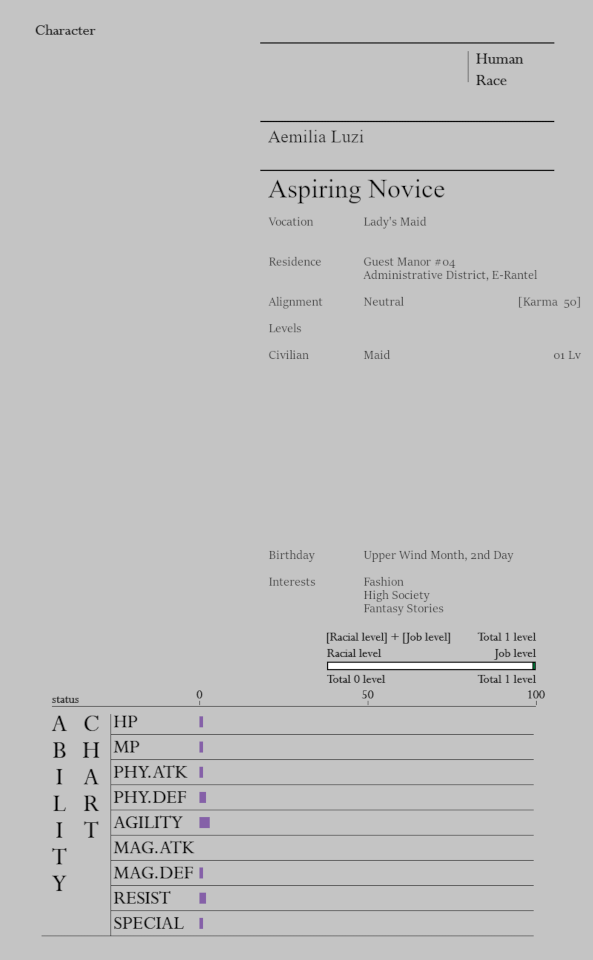
\includegraphics[width=1\linewidth]{V1 Birthright//images/NaUEKrB.png}
    \caption*{Aemilia Luzi Character Sheet}
\end{figure}

\section*{The Noble Household (Part I)}

The noble household employs a myriad of servants and retainers: from iconic Butlers and Maids, to Men-at-Arms, Cooks, Groundskeepers and Pages(to name a few). These individuals that serve the aristocratic estate are far from the shallow imitations that occasionally appear to work on an intermittent basis, functioning as some part of common hospitality to create a transient atmosphere of wealth and luxury. Members of a noble household are retainers which often serve as close personal attendants of noble families in all matters mundane.

 

In a world where fending for oneself often entails risk of debilitating injury, death or worse, a stable life in honoured service under the protection of a powerful family is an enticing prospect for those without the means to make their own way – or those confident that their skills in stewardship can be put to use leveraging the wealth and influence of a noble master.

 

Yet as menial as the lowest of these positions may seem, those with hopeful prospects must pass stringent filters; only those who are deemed suitable will be invited to assume the positions of trust that expose one to the inner workings of a noble house and the private lives of their families. Freedmen may enter into the lowest ranks of household hierarchy, while those of noble blood may start in roles that suit their education and upbringing. However, only those possessed of experience and talent usually rise to the highest positions of authority.

 

A noble's household may be seen as the family of vassals that most closely surrounds the family that they serve. While individually not as prominent as their Lords and Ladies, they are collectively the most visible aspect of a Noble House. They carry within them the honor, will and pride of their houses, representing them in the many aspects of daily life in a demesne.

 

Vampiric Households are a dark mirror of the noble household: bound to their master – willingly or unwillingly – in eternal undead servitude.



\chapter{Ludmila Zahradnik}

Ludmila hummed to herself whilst sitting in front of the large dresser mirror, slowly brushing out her hair with an old, reliable lacquered comb that had been in her possession since she was a girl. She wasn’t in a bad mood before, but the hot bath had put her into a much better one as surely as soaking in the warm water had lent the sensation of melting away the day’s stress and worries. Knowing that Lady Shalltear was already willing to assist her efforts to restore Warden’s Vale lightened the burdens weighing on her mind, and she now focused her thoughts on how one might best address the problems that she had seen and heard described in E-Rantel.

 

One of the maids brought in by Yuri Alpha hovered nervously somewhere to her side, holding a spare towel, while another was preparing her outfit for dinner. Judging by the sounds coming from below, there seemed to be a few others working around the manor. She glanced at the reflection of the maid waiting on her – it seemed like she had put at least some effort into maintaining her haggard appearance, but it felt mostly the same as the other residents that she had seen so far. The women were tired and frightened: long days in such a state had left them in a nervous and jumpy condition. When one of the Undead sentries provided by Yuri Alpha came stomping in with two barrels of steaming hot water, the both of them screamed and fled to cower in the furthest corner of the solar and stayed there. Ludmila ended up having the unique experience of instructing a Death Knight on how to draw a bath.

 

It was a long while after it had stomped back out of the room that the pair came out of hiding, and by then Ludmila was already half done on her own. Beyond that, the maids seemed very new at their jobs. In previous years, the city had similarly provided maids for visiting nobles who rented the guest houses and the current maids seemed to be quite unpracticed by comparison. Their movements seemed stiff and unsure; they seem to be constantly second guessing themselves as they worked. It was to the point that their insecurity was subtly affecting those around them, and Ludmila frowned as she had to mentally wave the feeling away. As Yuri Alpha had demonstrated earlier in the evening, confidence and form inspired the same in those around her, and so it seemed that the reverse was true as well.

 

Ludmila thought back to Vilette Jezne and her actions during the gathering of nobles. Perhaps her haranguing of the others was a different facet of the same idea: to provoke a sense of normalcy and routine that caused others to act out of habit. While she had no aspiration to become a crotchety old crab, Ludmila thought she might be able to achieve those same results in her own way. And so, she simply went about her preparations for dinner, methodically running down a mental checklist of her own routines as she moved about the room in her ongoing preparations. It did not take long until the two maids also started to move, trying to keep up with and eventually anticipating her actions. These maids had obviously undergone some sort of training, but they probably had no opportunity to put their training to work with the state of E-Rantel as it was.

 

She stood and waited in a fresh linen shift as the maids brought her dress to her. Though the hearth had been stocked and lit, the air in the room was still warming up. She suppressed a shiver as she mentally willed the maids to move faster. The dress had been purchased last winter, as a reward for her own hard work helping to organize the Barony that year. It was something she thought might suit both their brief appearances in E-Rantel as well as the few festive events at home. It had a pleated white cotton blouse, with long sleeves and black buttons which ran up and under the ruffled bow tie which spilled from the collar. A wide kidney belt fashioned from leather wrapped over the waist, separating the blouse from the long, three panel skirt made from linen dyed in forest green. An open bolero matched the skirt, decorated with buttons between the elbow and wrist. The dress was warm enough for winter in E-Rantel, and she only needed to wear a coat over it to be serviceable in the highlands.

 

It had been on display in the window of a boutique near the main plaza, and she spotted it while her family was on the way back from selling their goods at the various merchant warehouses in the outskirts – she immediately hopped off their moving wagon and bought it with over half of her earnings for the year. After she returned triumphantly with her spoils, her brothers had wailed upon hearing the cost of the entire outfit, as it was enough to buy half a suit of masterwork plate armour. Her father just seemed relieved that his only daughter was not just a tomboy after years of being raised in a household full of men.

 

As she was now helped into the dress by her maids, however, a vague sense of annoyance filled her as she saw that her ambitions of yesteryear had been somewhat misplaced. She had grown taller, causing the hem of her skirt to come two thirds of the way up to her knee. The pleated blouse did not fill out as much as she had hoped that it would, leaving it loose over her chest. Ludmila resisted the urge to sigh as the maids fussed over her appearance. When they were nearly finished, one finally spoke.

 

“Frontier Nobles really are amazing…”

 

Aemilia Luzi was the younger of the two maids, who had arrived and introduced themselves just before the Death Knight had come to deliver water for the bath. The girl was half a head shorter than Ludmila, with shoulder-length auburn hair and a face full of light freckles. Her emerald eyes glimmered as she continued.

 

“Even in a beautiful dress, you look like a gallant warrior at the same time. Everything about it suits you so well while making it seem like you could go to battle just like that. Even the hem of your skirt is raised so you can move around easily, when other ladies might have chosen a more reserved appearance.”

 

The excited maid made a motion with her right arm, as if she was swinging a sword, or perhaps clubbing someone with a rolling pin...or stabbing something with a fork? Ludmila could not tell.

 

“...how do you do it, my lady?” She asked.

 

Aemilia’s voice lost its excited tinge, turning subdued. Ludmila looked down at her dress, searching for any problems with the outfit. She didn’t notice anything wrong in the mirror, either.

 

“Do what?”

 

The maid’s work slowed, until her hands stopped moving entirely. She looked up to Ludmila with an expression that was a mixture of awe and uncertainty.

 

“How do you live your life like everything is normal?” She said, “I’ve heard some others talk about how they saw you walking outside this evening, all by yourself in the noble’s district like it was just a regular spring day. I thought that maybe that was an exaggerated rumor, but then that monster came into the room just now and you just continued on like nothing at all was strange.”

 

Ludmila opened her mouth, then closed it again, uncertain how to respond. She didn’t feel like she had done anything that anyone else couldn’t have. It wasn’t as if she never panicked, or did not feel fear or insecurity. Even her actions around the maids were just an experiment that she was not even sure would work or not, inspired by what she had experienced previously that day. She thought that a straightforward answer would be best.

 

“I don’t think I’ve done anything special,” she said, “and this is hardly normal for me. I was frightened at first, when I saw all of the Undead in the city, but then I realized that fear for its own sake was unreasonable. I simply decided that I had more important things to do; that I could not afford a life that had me jumping at every shadow. That the days and seasons would pass; that the world would continue to run outside of our borders. That in spite of all of my fears and uncertainty, I still needed to fulfil my duties to the land or my fief would fall to ruin.”

 

Aemilia’s eyes were sparkling again, but a dismissive sniff from Ludmila’s other arm indicated that the second maid did not see things the same way. Terah Ro'eh’s husky voice was about as incredulous as one could get without sounding outright disrespectful.

 

“You decided?” She said, “My lady, if we could all just get up one morning and decide to get back to life as usual, no one would be hiding in their homes now, would they?”

 

“She’s right,” Aemilia said reluctantly, “even the other nobles tried a day or two ago. A few of the ladies riled up one of the boys to show them how brave they were, so he marched out of the clubhouse with everyone following a safe distance away. He stormed right up to one of those Death Knights and soiled himself as soon as he came within a few strides, collapsing on the ground in a puddle. When the Undead monster turned to look our way, everyone screamed and ran all the way back to the clubhouse, leaving the poor nobleman lying on the street.”

 

Terah nodded at the other maid’s words, her black curls bouncing over the dusky skin of her cheeks.

 

“That’s right,” she said. “In the end, Miss Alpha had to carry him back to his manor. The poor kid was out cold. Mark my words: Frontier Nobles are made different, somehow. When times are good those other nobles might know how to boss people around, but all the boasting and bragging and talk of being brave captains and fierce fighters is like it never was when it comes down to it.”

 

Her attendant’s disdain for the rest of the nobility was alarming, to say the least. Ludmila felt a tugging obligation to at least salvage at least a little bit of her peers’ respect.

 

“Then what about Yuri Alpha?” Ludmila asked, “She doesn’t seem to mind everything that goes on. If anything, she seems to carry herself far better than I do.”

 

“You’re right, my lady,” Aemilia replied, “but...she’s one of the Royal Maids, you know? She’s probably had a long time getting used to all that, or maybe she’s not what she seems to be at all.”

 

Ludmila thought Yuri Alpha did not appear to be abnormal in any way, so she decided to follow up on the first idea.

 

“Then maybe all it takes is time,” she suggested. “The two of you seem to be gossiping quite bravely here, after all.”

 

The animated atmosphere instantly turned solemn as the two maids exchanged glances. Terah was the first to recover, glancing at Ludmila as she spoke.

 

“A little time then, my lady?” Terah said, “Maybe you’re right, but you still won’t catch me walking up to those Undead any time soon.”

 

“You...you won’t tell anyone about what we said before, will you, my lady?” Aemilia asked.

 

“Not this time, no,” Ludmila answered. “In the future, however, I will not defend you with falsehoods if you are caught slandering the Royal Household or His Majesty’s nobility.”

 

The two maids stood and stepped back, having completed her outfit. They curtseyed in unison as Ludmila stepped off of the dressing stool and headed out of the solar.

 

“Thank you, Lady Zahradnik.”
\chapter{Ludmila Zahradnik}

The night’s rain had ceased, and the courtyard patio glistened as Ludmila made her way back down the stairs to the main floor of the manor. The corridors were lit – as were the various rooms in use by the new members of the manor staff. She headed back towards the kitchen to see if Lady Shalltear was still there.

 

“Over here, Baroness,” she heard her liege call to her from off to the side.

 

Turning towards the sound of her voice, Ludmila spotted the edge of the black gown with its silver and carmine frills in a drawing room across the courtyard. She made her way around and into the room, coming upon Lady Shalltear who was nibbling on a scone. Seeing the food pass through the image of one mouth and into the other was odd, to say the least. Yuri Alpha was nowhere to be seen. Ludmila took a seat on a short sofa across the rosewood centre table from the Lady Shalltear, whose dangling feet were swinging idly under her skirts as she worked on her pastry.

 

A shallow splash in the courtyard turned their heads towards the entrance of the drawing room. Yuri Alpha had returned, with a covered dinner tray in hand. Shalltear’s sarcastic query met the maid as she entered the room.

 

“You’re not making a dynamic entrance like that every time you want to enter someone’s house, are you?”

 

“Of course not, Lady Shalltear,” Yuri replied. “I was simply repositioning one of the Hanzos from an empty manor nearby; the roof of this building should be better secured now.”

 

Yuri Alpha came over to lightly place the silver tray on the centre table.

 

“Please pardon my presumption, but I took the liberty of ordering your meal, Lady Zahradnik,” she said. “This should be popular amongst young people…at the least, Lady Aura seems to relish it.”

 

Yuri Alpha lifted the cover, and Ludmila leaned forward. An appetizing aroma was released into the room, but the food that lay arranged within was unfamiliar. There was something resembling a sandwich, while the rest of the plate was filled with golden strips. Bubbles rose out of the dark drink in the clear glass beside the plate. That it all seemed to maintain its neat placement was a mystery – especially considering the maid had jumped down from over two storeys into the courtyard.

 

“The sandwich is called a ‘hamburger’,” Yuri Alpha gestured with her hand as she described the meal, “I believe that potatoes are used in Imperial cuisine – those golden strips are called ‘fries’. The beverage is a sweet, fizzy drink called ‘cola’.”

 

Ludmila searched the tray for utensils, but there appeared to be none available to sample the exotic foods enticing her.

 

“This meal is usually eaten with one’s bare hands.” Yuri Alpha informed her.

 

Ludmila cast a look that begged askance at the maid, then she looked back to the meal, hesitantly fishing out one of the strips from the platter. While she had heard of potatoes before, she had never had the opportunity to try them.

 

The starchy food seemed to have been cut and fried in oil, then lightly salted. They had the same rough texture as arrowroot tubers from Warden’s Vale, but were decidedly less sweet and crispy. The method of preparation made them quite tasty, however – she wondered if she could do the same thing with the produce from her barony…though oil for frying was not a commonly available commodity in the highlands.

 

She reached out to bring the glass to her lips, then pulled her head back as the fumes from the drink burned the inside of her nose. After seeing no reaction from the two others, she gingerly took a sip. The sweet drink scoured her throat as she swallowed; she thought it was something that was definitely an acquired taste. The sandwich was a bit more regular – someone had taken minced meat of some sort and grilled it; there was a mixture of savoury sauces in the sandwich that complemented the smokey flavour of the meat. There were also both fresh and pickled vegetables inside, similar to ones she had tasted before. Having not eaten for most of the day, her ravenous appetite had her take all of five minutes to complete the meal while Lady Shalltear and Yuri Alpha looked on.

 

“I trust that you enjoyed the meal, Baroness?” Yuri Alpha asked as she retrieved the tray.

 

“It was very satisfying, thank you,” Ludmila replied. “Especially these fried potatoes…I think something similar could be done with produce from my demesne.”

 

She struggled not to burp as Yuri Alpha looked at her expectantly.

 

“You didn’t…feel anything?” Yuri Alpha said, “The sensation of becoming stronger, or perhaps more robust?”

 

“What do you mean?” Ludmila asked.

 

“The meal should have several beneficial effects upon consumption,” she explained, “though admittedly, Lady Aura does not particularly care about the effects, only the flavour.”

 

Ludmila shook her head, then eyed the half-emptied glass on the table. Did she have to finish the whole meal, including the drink? She had never eaten a meal that provided benefits immediately after consumption. The Sorcerous Kingdom surely had a variety of wondrous things she had never heard of before.

 

“That is quite curious,” the maid said. “I believe the other chefs will find this information of great interest.”

 

Yuri Alpha turned her attention to Lady Shalltear.

 

“If I may ask, Lady Shalltear,” she asked, “how were your scones?”

 

“One was the same, as usual,” Lady Shalltear replied. “The other tasted a bit strange…you should know as well as I that I won’t gain anything from eating them, though.”

 

“We can never be too certain here,” Yuri Alpha said, “and the chefs are being quite thorough in their investigations. There are still many recipes and local ingredients left to cover – any one of them could turn up with something unexpected.”

 

With a slight bow, Yuri Alpha left with the dinner tray, disappearing into the corridor.

 

Her hunger sated, Ludmila leaned back slightly into the sofa, looking across the table at Lady Shalltear, who had long since finished her scones.

 

“So…are you refreshed and ready to work now?” Lady Shalltear said, “There is much to be done ahead of us.”

 

She seemed eager to begin yet, when Ludmila looked around them, there were only crumbs from Lady Shalltear’s snack on her side of the table.

 

“I am still unsure what exactly you have in mind when you say that, my lady,” Ludmila said. “I have some experience in helping to manage my father’s demesne, but I do not know what His Majesty expects of me in my position as a minor noble.”

 

“Well, the discussion didn’t say anything in particular of what they wanted from you, just that you could provide assistance in getting things going again. Did your former liege always tell you what needed to be done?”

 

Now that she mentioned it, Ludmila realized that she may have overestimated the scope of what had been said earlier. The nobles of Re-Estize were by and large autonomous rulers within their own fiefs – only occasionally collaborating with others to tackle their common interests. Similarly, it was rare that they would be called to assist in their liege’s matters; only those exceptional enough to qualify as ministers and proxies were appointed to such important positions. Ludmila had only started to help manage her own family’s territory when she was twelve – mostly in limited capacity until recently – so what was required of her probably had to do with something within her limited experience.

 

“If it is something that has to do with my own demesne,” Ludmila thought it a good time to disclose her own situation, “then I will need to attend to several pressing issues that can only be addressed in E-Rantel. My territory is vacated, so I need to find new migrants that can survive life on the border. Then, based on the numbers that can be convinced to immigrate, I will need to purchase tools, parts and various necessities for living on the frontier. Momon sent my village’s goods…somewhere; I must track him down somehow and find out where they went. Depending on the prices I receive for those goods and how many I need to provide for, I might need a subsidy if there is a shortfall…”

 

Across from her, the Vampire’s bright, crimson eyes seemed to have gone dull. It reminded her of the times when she would speak to her family on these matters – as comprehension decreased, so did their attention span. It usually took her until she got to the strings of figures in her reports to achieve the same effect with her father and brothers, though.

 

Yuri Alpha cleared her throat to the side. While Ludmila spoke, she had been cleaning the table, taking away the remains of the meal and replacing the tablecloth. A tea set was laid out before them on the table, and the maid spoke as she poured out cups of fragrant red tea for them.

 

“I believe you will find the methods to apply for everything you need in the forms and reference materials that have been prepared for the local administration by Lady Albedo,” the maid said.

 

After placing an expensive-looking teacup with floral designs traced over it before Ludmila, Yuri Alpha produced a stack of books and folders from somewhere. As with Lady Shalltear’s parasol, they were seemingly taken out of thin air – Ludmila wondered if it was a magic item or spell common to the Sorcerous Kingdom. The maid gently placed the collection of items on the table but, even so, Ludmila could hear a light thump as the mass was released.

 

Lady Shalltear eyed the pile with the same look that a person might have given to something distasteful.

 

“I thought Albedo didn’t want anything to do with us,” she said.

 

“You should know as well as I that Lady Albedo has prepared extensively for this, Lady Shalltear,” Yuri Alpha replied. “These materials are made readily available to any who would take up related matters in the civil office anyways, so I thought it prudent to save time by picking them up in advance.”

 

As Yuri Alpha finished arranging the items on the table, Lady Shalltear shifted over on her seat. The maid rose to stand beside the sofa, and the Vampire patted the cushions in the space she had made for her, smiling up hopefully. Yuri Alpha pointedly turned her head away in refusal, choosing to remain standing to the side.

 

The brief exchange left Ludmila wondering what the relationship between them was. Even a maid in the service of royalty would be hard-pressed to evade the suggestions of a high noble – much less outright refuse them – as their reception could be perceived as a reflection of their master’s disposition towards said noble. The resulting interpretation of this behaviour could cause no end to the troubles between a host and their guest, and so those in noble employ would constantly need to be aware of the will of their master and perform in a manner appropriate to the expression of their many associations.

 

Though Lady Shalltear had a look of disappointment on her face, it seemed that she had treated the refusal as nothing more than a part of their regular interactions. The way in which Yuri Alpha pressed Lady Shalltear when she discovered the two in the kitchen was also at odds with how a maid would normally act towards a member of the Royal Court. Some might have construed His Majesty's disapproval or even ill-will in Yuri Alpha’s actions towards her.

 

Perhaps the elegant maid held some other position even as she served as part of the royal household. It was not uncommon for unmarried noble scions to enter in such service that suited their station and, going by the dignified atmosphere that always seemed to follow her, Ludmila would not be surprised if the maid was in reality a princess from some other part of the Sorcerous Kingdom. As she studied her face, Yuri Alpha betrayed no indication that could be seen as evidence of her speculations being correct – she simply looked back at Ludmila expectantly, patiently waiting for her to examine the various items that had been placed on the table.

 

Ludmila reached out to take the first folder from the stack in front of her. Within, she discovered what appeared to be forms, drafted in impeccable, uniform script. As she leafed through dozens of them, they all appeared to adhere to the same stringent standard. The clean lines and consistent handwriting over so many documents made the whole feel like an artform in itself – she had never seen the like in her life.

 

They were written to be clearly understandable, though she occasionally came across terms that were entirely foreign to her. Each form was made to assist in requesting articles that were needed in the various industries of the duchy, from the smiths, tailors and processing facilities in the city, to rural activities like farming, mining and logging. There were even those for warehouses, restaurants and various commercial services that were usually left on their own to sort themselves out.

 

“Amazing,” Ludmila remarked as she continued to flip through the documents. “Were these all drafted by a single person?”

 

“The Guardian Overseer created the templates for these, yes,” Yuri Alpha said. “Since then, the work to create copies of them has been handed to administrative assistants.”

 

Yuri Alpha leaned over from where she was standing, selecting a booklet among the items on the table and offering it to her.

 

“If there’s anything you don’t understand,” she said, “this is a glossary for terms that may not be familiar to the people of this region.”

 

Ludmila placed the booklet on her lap and reached for the next folder. The files within appeared to be for calculating and reporting taxes. The last folder contained requests for military assistance. Her eyes widened as she skimmed over the list and encountered Death Knight, Elder Lich and Soul Eater. Recalling that Bohdan had speculated that the legendary magic caster Fluder Paradyne may have become an Elder Lich, she wondered if all of the assets on the various forms were similar. Would all of the Sorcerous Kingdom’s nobles be allowed to field armies filled with creatures of legend? One could easily carve out their own nation with such overwhelming military might. Raising the folder with her left hand, she posed a question.

 

“These seem to state that we can request extended deployment of the Sorcerous Kingdom’s military forces…but there must be limitations?” Ludmila asked.

 

Yuri Alpha adjusted her spectacle frames, putting on a stern look.

 

“Requests for these deployments must be justifiable,” she said, “and for security measures only. Use of His Majesty’s forces in a belligerent manner on an international scale is prohibited by his servants. They are also issued with contingency orders for various events and outcomes, so understand that any attempt to wage war against friendly territories with them will not work and may result in fines or other disciplinary measures if warranted.”

 

“…of course,” Ludmila said. “I was just making sure that there were measures in place against abuse…I was not planning on conquering the Slane Theocracy any time soon.”

 

Lady Shalltear looked up with interest while Yuri Alpha furrowed her brow.

 

“It was a joke,” Ludmila replied hurriedly – perhaps being too serious led to her own brand of humor being taken seriously as well.

 

She shifted uncomfortably in the silence that followed, looking to what was left of the pile on the table. There were four large books – it would not be incorrect to call them tomes – and lifting one felt akin to picking up a block of heavy wood. Placing them side by side, she read the titles on their respective covers: Agriculture, Forestry \& Extraction, Refining \& Manufacture, Commerce \& Hospitality. Reaching out with both hands, she pulled the book labeled Agriculture onto her lap.

 

Within, the pages had been divided into clear halves. One side had been partially filled, listing various agricultural products – both plant and animal as well as intermediate goods related to the industry. Each had its own section in the column, listing supplementary products, such as fertilizer, feed and tools. It came with recommendations for many, but as she leafed through the pages, Ludmila discovered that there were far more blank spaces in each section.

 

The other half of each page was a template meant to be filled in with results: crop and herd yields, as well as space for feedback on the information provided and special concerns. Ludmila already had a fairly clear idea as to what was being asked, but she reached over to lay open the three books on the table to confirm her thoughts. Like the one on her lap, they all displayed a similar format.

 

Each was a sort of makeshift almanac, but there was a lack of information to provide proper forecasts and recommendations. The Sorcerous Kingdom had retained the laws that governed the nation, but the civilian administration had undergone changes to the point where the whole would not be recognizable to what had come before. The new administration needed a bare minimum of functional industries in order to test its new methods and enact policy, but the apparatus had essentially been jammed with the sudden annexation of the duchy and the new realities that came with it.

 

“Do you understand what needs to be done?” Lady Shalltear asked after Ludmila looked back up at her.

 

“I do, my lady.” Ludmila said. “Well, believe I understand what is being asked by these, and I know what needs to be done to achieve what is being asked.”

 

Lady Shalltear and Yuri Alpha had been waiting patiently while Ludmila perused the contents of what had been set before her, and they brightened visibly upon hearing her words. Ludmila had no illusions that remedying the entire situation would be as simple, though.

 

“In order to return the duchy to normal,” she continued, “the people need to understand what the new normal is. With stability and certainty comes confidence; only then will the population come fully back to life. It is something that will take time, but someone has to start somewhere…”

 

As Ludmila leafed through the incomplete almanac on her lap, a sudden thought gripped her.

 

“Say, how is the city doing for food and supplies?” She asked.

 

“When this city was annexed,” Lady Shalltear responded, “the provisions that the Royal Army of Re-Estize had stored in the warehouse were abandoned, so they were seized by His Majesty’s forces.”

 

“How large was the levy this year?”

 

“One quarter million, roughly.”

 

Ludmila did a quick calculation in her head. While rural territories might be able to forage or glean food from their surrounding fields and forests, the ability for the uncultivated lands to support the inland population would quickly diminish and they would still need to be supplemented with food until seasonal activities returned to normal. The city had no such option, relying on imports entirely. The needs of an army and the needs of the citizenry were vastly different, but food and fuel were still the same.

 

“One year,” Ludmila frowned.

 

Lady Shalltear and Yuri Alpha looked at her curiously.

 

“One year?” Lady Shalltear frowned back.

 

“The annual skirmish with the Empire usually lasts four or five weeks, not including the time to organize and station the levy,” Ludmila explained. “The Kingdom brings enough provisions to E-Rantel for roughly six months. This is enough to feed the city and army long enough for emergency relief to be mustered and arrive from the Kingdom in the event of a siege. With the city in the state that it is in, various tools and parts associated with city life will mostly not wear down since they aren’t in use, but the people still need to eat and stay warm. The excess food from the harvest in the inner territories would have probably gone towards this stockpile, so the duchy has a little over one year of food available. Even in the best case scenario, a late planting season will mean that the territories won’t have the same crops that they usually do. We will need to restore operations quickly to avoid this, or at least produce enough so that trade can make up for our shortfalls. If we do not, the duchy will starve next spring.”
\chapter{Ludmila Zahradnik}

Ludmila stirred to the sound of work being done downstairs. The drapes of her solar had been drawn tightly shut and the door to the hallway was closed, but the bustle of the maids on the ground floor preparing for the day still carried through from the open courtyard of the manor. She stretched herself under her covers and tried to rub the sleep out of her eyes.

 

It had been well past midnight when Lady Shalltear and Yuri Alpha left together. Upon hearing that Ludmila had an idea of what the various documents were asking for and what needed to be done, her new liege had wanted to start immediately. Yuri Alpha, however, reminded her that Humans tired out and it would be best to resume after a period of rest, so Lady Shalltear had hesitantly agreed to pick Ludmila up from the guest house in the morning.

 

She slipped out of bed and padded over to the window, parting the drapes slightly to look outside. Though the rains had stopped before she had retired for the night, the skies remained overcast and a grey pall was cast over the district. She was accustomed to rising after daybreak, but it was still dark enough that the streetlamps had been left on. Looking down to the front of the building, she saw the two Death Knights standing guard at the street entrance.

 

There was a light tapping at the door.

 

“Yes?”

 

“Baroness Zahradnik,” Aemilia’s voice sounded through the door, “you requested a morning call an hour after dawn.”

 

“I’m up," Ludmila replied. "Thank you, Luzi.”

 

Ludmila stepped back from the window, letting the curtains fall back down again as the maid opened the door. The courtyard was still being artificially lit in the morning gloom; the air carried with it the smells of woodsmoke and of breakfast being prepared. Aemilia closed the door behind her, then turned to curtsey.

 

“Good morning, Lady Zahradni–oh my, it’s pitch black in here!”

 

Ludmila watched as the maid groped about blindly – it seemed that yet another of the qualities of her Talent that Lady Shalltear had described the previous night was true. Humans could not normally see in the dark; she wondered how she could have thought otherwise for so long without realizing it. Before Aemilia could topple any of the furniture in the solar, Ludmila drew open the curtain again to dimly light the interior. The maid immediately straightened, walking about cautiously in the weak illumination.

 

“Oh, you should let me draw open the rest of the windows, my lady,” she said. “If I recall correctly, there was an appointment you needed to get ready for soon?”

 

“Yes,” Ludmila replied, “they said that one of the fellows posted outside the door would deliver word to them once I knew when I'd be ready. Is everyone else up? I should have one of the other maids let them know.”

 

“Terah chased the other two out of bed a couple of hours ago...um, I don’t think any of us will be able to approach the guards outside, my lady. I’m sorry.”

 

“That’s fine for now. I’ll inform them before breakfast.”

 

Ludmila sat down in front of the dresser mirror and looked around for her comb. The maids had unpacked her things the previous evening, but her personal belongings seemed rather meagre in comparison to the luxurious counter they were laid upon. Before she could reach out to pick it up, Aemilia swooped in and snatched it from the counter.

 

“Please let us take care of you, my lady,” her voice quavered a bit as she started to work on Ludmila’s appearance.

 

Aemilia appeared somewhat slow when it came to herself, but her maid was astonishingly quick when it came to her mistress. Resigning herself to Aemilia’s attentions, she reached out to take one of the files left behind by Yuri Alpha. Before going to bed, Ludmila had sorted out the forms that she thought would be relevant to Warden’s Vale. Though she had referred many times to the reference booklet and the incomplete almanacs that had been included, there were several things that still eluded her comprehension.

 

The process by which everything was filled out was relatively straightforward. One needed to identify their fief’s products, cross reference them with the provided almanacs and fill out the relevant forms. Based on the area of the land being utilized and the projected yield, an applicant would then simply tabulate their needs and write them down. At least it would have been simple, if the references were fully completed. Of all the produce listed in the agricultural almanac, only a handful of the more common crops had been filled out completely – namely several types of grain and potatoes.

 

Warden’s Vale had several old terraces cut into the lower slopes of the valley near to the village – remnants of a time when the barony was still in a position to develop its lands. The hamlet constructed to house field workers had long since fallen into disrepair, and only the nearest portion was left in use. After re-clearing all of the old and fallow fields, they would have roughly four thousand acres to work with. She had referenced the material for Oats, which did well in the cool, moist weather of the highland valley. It was a straightforward calculation but, at this point, several questions arose.

 

The numbers did not make much sense to her. The final tabulation had resulted in eighty light units of labour and four heavy units of labour. But no matter how she could frame these numbers, there was no way eighty tenant Farmers and four teams of draft horses or oxen could work such a large amount of land. A team of draft horses with a wide plough could perhaps cover seven acres in a work day, and four teams would take around five months to till four thousand acres after weather conditions were accounted for. There was also the matter of keeping the land clear and harrowing the tillage…Farmers in the lowlands might have been able to accomplish this with their mild winter climate, but the highland soil would become cold and unworkable in those months.

 

Similarly, she could not picture eighty tenant Farmers being sufficient to maintain and harvest the entire area. At the end of each growing season, the harvest would not be fast enough with what she saw allotted. Perhaps the Sorcerous Kingdom employed magical tools to expedite farm work, but in none of the nations surrounding Re-Estize was this practiced. She would have to take up her concerns with the civil office – hopefully, they would be able to provide clarification.

 

Her difficulties grasping what methods were being employed made the other parts even harder. The majority of the products of Warden’s Vale were harvested from the marshy flats that covered the floodplain of the valley. Rather than being farmed, it would be more accurate to say that they were foraged as there was no work put into planting. The villagers only needed the knowledge and expertise, which was a part of a Ranger's training, to harvest the various plants that grew in the valley throughout the seasons. Until she knew what the realm was providing with these application forms, she could not rightly estimate what she needed to perform these tasks.

 

There were several other documents involving forestry, which met with the same problems. While the application for logging was fairly straightforward, foraging edible products, herbs for medicines and several luxuries such as spices, pigments and plants used for cosmetics had no such detail in the Almanac. At the end of it all, she was dismayed to find that only one third of the documents had been filled out sufficiently, while the rest simply had little to no material to cross reference. The entire system had the sense of being developed for some other place, and they were now attempting to implement it throughout the duchy. Even the terminology required a glossary for an applicant from Re-Estize to interpret.

 

“Your dress is ready, my lady,” Aemilia said quietly behind her.

 

Ludmila turned her head towards the sound of Aemilia’s voice. Her outfit from the previous evening had been cleaned up, ironed out and placed on a mannequin stand. The amount of care that the dress had been given by the maid made Ludmila feel slightly guilty for keeping it packed up at the bottom of her trunk for months at a time.

 

“Shouldn’t I have breakfast before putting it on?” Ludmila asked, “I don’t want it collecting crumbs and smelling like bacon after all the work you did.”

 

Aemilia made a face, then walked over to check through the tall chest of drawers where her clothing had been sorted into. It didn’t take long before she turned back – everything she had brought for herself shouldn’t have even filled one of the drawers, after all.

 

“Aside from this dress,” she said, “I found your outfit for travelling in the country, plus some smallclothes…don’t tell me you plan on walking around in your chemise?”

 

“Yes?”

 

“No. Nonononono,” the maid’s voice went up in scale by two notches, “one does not simply walk around a manor like that. It is absolutely improper for a noblewoman. Allow me to bring breakfast up to you here, my lady.”

 

“I don’t want this room smelling like food,” Ludmila told her. “No one seemed to mind my walking around the manor in the barony, anyways.”

 

Aemilia frowned at her claim, turning to face her with a tentative expression.

 

“And just who did you share your manor with, precisely?” She asked.

 

“With...my family?” She replied, “My father and brothers, and any villagers that came in to take care of things – usually patrolmen in training with duties assigned to them. The priest’s acolyte, as well.”

 

Aemilia’s eyebrows shot up to match the tone of her voice.

 

“There are limits to being brave, my lady,” she said. “Perhaps it’s something that you’ve become accustomed to from your childhood, but an eligible young lady such as yourself should not be displaying herself to men in such a brazen manner…don’t tell me you were planning on speaking with the Death Knights like that?”

 

Ludmila suspected that answering her maid’s question would not end well, so she shrugged slightly. Her attempt at evasion didn’t work.

 

“Absolutely not!” Aemilia was aghast, “Standing out in the street like that…not to mention speaking to those fearful Undead guards in nothing but a scant piece of cloth!”

 

“I don’t think the Undead really care for that sort of thing…”

 

Undead aside, Ludmila thought the sensibilities between Aemilia and herself were a bit too far removed from one another. Rural villages were composed of homes which were essentially large, shared spaces, so privacy was not really anywhere on the list of luxuries with that sort of lifestyle. Her ‘manor’ in Warden’s Vale was no different in this regard.

 

“Who’s to say? I’m no expert on the Undead, my lady, but who’s to say that there aren’t some lascivious ones out there?” The maid shuddered after the words left her mouth, “Well thanks for that thought, my lady.”

 

Ludmila wanted to point out that it had been entirely Aemilia’s own doing, but seeing that her maid had stopped accosting her over her appearance and lapsed into the gossipy tone that she carried after they first met, she counted it as a win of sorts. Setting her papers aside, she stood back up and the maid helped her into her dress.

 

“I'll need an attendant for the outing,” Ludmila said as Aemilia was making some final touches on her appearance. “Will you accompany me?”

 

“Of course, my lady!” Aemilia immediately brightened at the prospect, but her expression grew shadowed just as quickly. “Where are we going? The rest of us were busy making the place livable; all I could tell from your meeting yesterday evening was it had something to do with this monstrous pile of paperwork you have here.”

 

She motioned to the stack of books and file folders filled with documents. Ludmila pressed her lips into a thin line: she didn’t like the idea that others would listen in on official business like that, but she wasn’t sure what measures she could take against it in the future.

 

“Yes,” she said. “I need to turn in these forms to the civil office and meet with an official to clarify some things. In addition, I’ll need to deliver my fief’s goods to the merchant warehouses to sell. Then, there are some purchases to make based on what I can secure from the administration with these requests.”

 

The young maid, having already agreed to accompany her, now looked a bit cornered. She obviously knew something that Ludmila did not.

 

“What’s wrong?” Ludmila asked, “You seemed excited to accompany me at first.”

 

“That’s…well,” Aemilia licked her lips apprehensively, “the Sorcerous Kingdom has replaced the missing administrative staff with Undead, my lady. I’m not confident that I can stride boldly into a building full of them like you can.”

 

“Well, you can wait outside if you don’t feel up to it,” Ludmila said. “I wanted you to help out with some personal articles, mainly. I need to replace old clothing that I’ve grown out of as well as find new pieces for daily use.”

 

Aemilia perked up a bit at her words. Ludmila had laid out the prospect considering her maid’s attitude earlier about the lack of a wardrobe, and it seemed to have some effect.

 

“Alright, I’ll take another look at your things and figure out what you need while you have breakfast,” the maid made some last-minute checks on the dress, then stepped away. “We’re done here, my lady. Please enjoy your meal.”
\chapter{Ludmila Zahradnik}

After informing Terah that she would be having her breakfast in the drawing room, Ludmila walked down the main corridor to the entrance of the guest house. Judging by the appearance of the patio as she passed by the courtyard, the streets would still be damp and gloomy. She opened the front door and walked up to where the two Death Knights faced the street at the end of the lane by the letterbox.

 

Looking at all the spikes on their armour, it seemed a hazard to even attempt passage between the pair of towering sentinels. Standing behind them on the path leading from the door, she cleared her throat just loudly enough to be heard, and the one to her left turned to look in her direction. It did not move like a Human normally would, instead twisting its body around with the joints of its dark armour somehow allowing the uncomfortable looking action. The web of red veins that ran over the black plates made its armour seem more like a carapace, pulsing with malignant energy. Its baleful crimson gaze turned down to meet her own, much the same way as the one in the streets did the previous evening. Maybe they just looked that way all the time. She shifted to face her Undead footman.

 

“Inform Lady Shalltear that I will be ready to meet with her in an hour,” she said. “There will be a single maid from my household accompanying me.”

 

Without awaiting anything further, the Death Knight marched off. Its partner moved to occupy the position that had been left vacant, purposefully stepping over to the other side of the lane. It seemed that every one of them wielded their weapon on the right – the tower shield it held would have blocked its line of sight to the entrance it was guarding if it had stayed where it was. Not only were these Undead frightening and powerful in appearance, they seemed to display a measure of competence as well.

 

After looking into the letterbox and finding it empty, Ludmila returned into the guest house, closing the door behind her. Breakfast had already been set in the drawing room; it seemed that Yuri Alpha had left the ornate dinner tray with its polished cover behind to be reused. She was greeted by fresh bacon and fluffy white bread with a dish of butter on the side. It was very different from the village stew she was used to; there was a distinct lack of greens…and everything else. She wondered if it had anything to do with the supply situation in the city, or if it was just what her maids considered a regular breakfast. Her father had always insisted they prepare the same stew that he had become accustomed to – going so far as to bring all the ingredients along on the trip – so she had never experienced the local breakfast before.

 

After finishing her meal, Ludmila decided that her father had the right idea. While the light breakfast had a refined feeling which was complemented by the tea served by Terah, it felt insufficient for the active lifestyle that she was used to. She suspected that she might end up having lunch early to make up for it.

 

Terah spoke while coming forward to take the tray away.

 

“If you have a moment to spare, my lady,” she said, “the other two maids would like to make their introductions.”

 

“How are they?” Ludmila asked, “I’ve heard they’re still having difficulties adjusting to life here.”

 

Terah harrumphed dismissively.

 

“No more than Aemilia and I,” she said. “It’s no excuse to hide under your covers until you start growing mold. They sure as hell started working once I threatened to make them stand outside with the guards.”

 

The older maid coughed, smoothing out her rough tone.

 

“That is, they’ll be useful to you in short order my lady,” she said mildly. “Ever since we’ve entered your service, things have started to become, well, more normal. You had the gist of it yesterday, I think…all it’ll take is time. As more people resume their lives, the more others will be compelled to do so.”

 

Ludmila wasn’t sure if Terah meant the act that she had put on for them yesterday, their short discussion, or both. Even so, she took it as a sign that she was on the right track when it came to getting the people back on their feet.

 

“Show them in, then,” Ludmila told her. “I’ll be away for most of the day, so it’s probably best to do this while we have the chance.”

 

She rose from the couch as Terah motioned for her fellow maids to enter. They were of an age and height with Aemilia, perhaps slightly older. The two were remarkably similar to one another: both sported shoulder-length dark teal hair, with pale faces and paler expressions. Dull grey eyes peeked out from under their bangs at her, then shifted away when she looked at them directly. They seemed dangerously thin, even under their voluminous maid uniforms.

 

“You’re being rude to the Baroness, girls.”

 

They jumped at Terah’s words, curtseying before Ludmila. The older maid sighed.

 

“Please forgive them for their behaviour, Lady Zahradnik,” she apologized. “These two are the Linum sisters: the one on your left is Wiluvien, Lluluvien is her younger sister.”

 

“We are at your service, Baroness Zahradnik,” they greeted her in unison, albeit timidly.

 

As they rose, Wiluvien gasped as Ludmila reached out and cupped her cheek, tracing her fingers up her jawline before lifting her hair to reveal her ears.

 

“Elves?” Ludmila murmured absently. She had never seen them before, only recognizing their telltale features.

 

“H-half-Elves, my lady,” Lluluvien spoke as her older sister trembled under Ludmila's touch. “We’re sorry, my lady.”

 

“Why are you apologizing?” Ludmila frowned.

 

“I’m sorry, my lady. It’s…I’m sorry.”

 

Ludmila withdrew her hand from the quivering Wiluvien, casting a questioning look at Terah.

 

“Did something happen?” Ludmila asked.

 

Terah sucked in her lips as she appeared to think on how to answer. There was clearly something going on with the two sisters, but it seemed she was a bit reluctant to share what she knew.

 

“I’m not sure if you’ll want to hear this my lady,” the maid said.

 

“This whole buildup certainly seems to beg the question.”

 

There was a pause as Terah looked to the sisters, then back at her. Her mouth worked behind closed lips, as if she was still trying to work out what she would say.

 

“Speak,” Ludmila said sharply.

 

She was growing impatient. Some time had passed and she expected someone to arrive to retrieve her at any point.

 

“They were in the service of Count Fassett,” Terah said. “The two sought refuge within the city after the battle.”

 

“That doesn’t sound bad at all,” Ludmila said, “why would you deliberate so much over that?”

 

“They weren’t maids, my lady,” Terah replied, “…they were his bed slaves.”

 

“Slavery is illegal, Mrs. Ro’eh,” Ludmila’s voice was stern. “Both in Re-Estize and the Sorcerous Kingdom.”

 

Terah shrugged, as if Ludmila’s statement could simply roll off of her shoulders.

 

“I don’t know much about laws, my lady,” she said, “but that’s what they were. Count Fassett was a powerful man in the duchy – as long as he was discrete, no one could gainsay him.”

 

Ludmila narrowed her eyes at Terah’s words. Her father had been wary of the man and shared his thoughts with his children, but she never imagined that the Count went so far as to flaunt the Crown Laws – something did not seem right. She turned her attention back to the sisters.

 

“Are Mrs. Ro’eh’s words true?” She asked.

 

“...she speaks truly, my lady,” Lluluvien hesitantly answered for the both of them.

 

“How did you come to be where you are now?”

 

“Our mother was a slave as well,” Lluluvien replied. “We were born slaves.”

 

Ludmila blinked several times at the reply, but it wasn’t the answer she was seeking. She rephrased her question.

 

“What I meant was: what happened that led up to your seeking refuge here?”

 

The Half-Elf maid looked up fearfully at her, and Ludmila saw herself reflected in Lluluvien’s eyes. She didn’t think her face was that scary – why were they so frightened?

 

“T-the Count…he sent us out to the military district to entertain his men a few days before the battle,” Lluluvien explained. “We were still there when the survivors came rushing back to the city, fleeing for their lives. Seeing how much confusion and panic there was, we went and vanished into the city, planning to escape when we had the chance.”

 

Lluluvien swallowed, staring at something in her memory.

 

“Except that chance never came. This city is now ruled by the Undead and we thought there was no way for us to survive when we saw that there was no work to be had. We returned to the Count’s manor here in the central district when we found out he had returned to the city, hoping he would take us in again…but he disappeared that very same day, and no one knows what happened to him. His household wouldn’t let us in, either. Miss Alpha found us on the street near to the manor, and she offered us the chance to work as maids in the city.”

 

Though it was an act born of desperation, Ludmila found it remarkable that they had made their way to the middle of the city when the regular citizens would not even leave their homes out of fear of all the Undead stationed in the streets. With how frail and frightened they appeared to be before her, she would not have imagined that they could.

 

“Are we fired?”

 

Ludmila looked back to the source of the voice.

 

“I’m sorry, my lady,” Lluluvien said quietly. “Are we fired, my lady? Women such as us...we aren’t qualified to serve as maids, are we?”

 

Ludmila knew that they were correct. Women of their background would not be considered suitable as maids, even in the loose sense of the profession in the central district. While she did not expect any of the hired maids here could even measure up to true maids of noble households like Yuri Alpha, their disreputable history also disqualified them even as temporary hired help. If the royal maid had not personally taken them in, they wouldn’t have even warranted consideration for training.

 

She glanced to Terah, who stood stone-faced to the side – there would be no feedback from that front. It was a conundrum where the Linum sisters’ unasked-for circumstances ran counter to their will to create a future free of that past. If Ludmila was not in such a sensitive position, she would not have any issues with taking them with her to Warden’s Vale to create new lives there. Such as it was, however, having second-generation bed slaves in her employ was both inconceivable and improper. The scales of her judgement, unfortunately, leaned clearly to one side: against her personal feelings on the matter, and she sought some way to reach an agreeable outcome.

 

She turned to examples, searching for some pretense from the past or present, and eventually thought of the previous evening in the cramped alleys of the city. Lady Shalltear had reached out to tend to the battered and sick harlot, in plain view of a throng of bystanders. It had sent a powerful message to the people, herself included. Even the city temples that she knew of might have shown open disdain for the woman, perhaps only tending to her out of sight in order to avoid unwelcome speculation. Yet her new liege had done so in complete disregard to her station as a direct vassal of the Sorcerer King and to her office as a high-ranking member of the clergy. She was in a position of incredible political power but she cared nothing for appearances – only for the will of her sovereign.

 

If her benefactor was willing to interact with a prostitute, then Ludmila could not rightly turn down slaves trying to escape a similar fate.

 

“I would like to speak with Yuri Alpha about a few things,” she said, “but no, I do not intend on immediately dismissing you. We should also have a priest examine the two of you to ensure you are healthy after your ordeals.”

 

Wiluvien turned her face up to look incredulously at the words. Lluluvien brought her sister close as she turned tearful at Ludmila’s response.

 

“Yes, my lady!” They cried, “Thank you, my lady!”

 

The sisters kept bowing and thanking her – it was already feeling awkward after the first few seconds. Fortunately, the doorbell rang from the maids’ office. Terah turned and headed out to answer, leaving Ludmila with the two Half-Elven sisters who continued with their wholehearted show of gratitude.

 

“What’s the delay?”

 

Lady Shalltear’s voice sounded from the hall, and she entered the drawing room with a pair of her beautiful attendants at her heels. Ludmila turned and stepped forward, presenting herself respectfully.

 

“Good morning, Lady Shalltear,” she said. “Thank you for personally coming to retrieve me.”

 

The maids, realizing that their mistress was addressing her own superior, immediately followed suit. Wiluvien and Lluluvien had already been halfway to their knees thanking Ludmila, and ended up with their faces to the rug. Lady Shalltear leaned to the side to look around Ludmila at the maids prostrating on the floor.

 

“Training your servants is all well and good,” Lady Shalltear said lightly, “but didn’t we have an appointment?”

 

“That’s not what I was doing–actually if you don’t mind, my lady, could you check the health of these maids?” Ludmila asked, “They’ve been through a bit of a…a…thing.”

 

She faltered at the end of her request, unable to provide an appropriate euphemism for their circumstances.

 

“If that’s all that’s holding us up, I suppose. Hmm…”

 

Lady Shalltear circled around to look down at the nearly prone maid sisters.

 

“You may rise,” she said.

 

At her voice, the Linum sisters’ kneeling forms unfolded and they sat up. Looks of awe appeared on both of their faces as they laid eyes on her peerless beauty. Without Ludmila’s Talent inadvertently tempering their reactions with her hidden appearance, she supposed this sort of enthralled state was to be expected.

 

“Well, beyond being nervous and fatigued, she hasn’t sustained any damage to her body.” The Cleric said absently as she shifted her gaze from Wiluvien to Lluluvien, “This one is also uninjured, except…ew?”

 

Lady Shalltear turned back to Ludmila. Even her monstrous appearance lurking under the enchanting visage seemed to portray a bit of disgust, somehow.

 

“Where exactly have these girls been?” She asked.

 

“They were sent to serve as…company for one of the nobles’ men in the military district,” Ludmila answered, “in the days leading up to the battle that took place at Katze Plains.”

 

“Were they intimate with anyone after that?” Lady Shalltear continued her queries, “The last thing we need is a city full of disease on top of everything else.”

 

Ludmila looked to Wiluvien and Lluluvien. They shook their heads vehemently and Lluluvien spoke, flush with embarrassment.

 

“No, my lady–my ladies?” She said, “After all t-that, we wanted to avoid it as much as possible, but…how did you know?”

 

Lady Shalltear had not appeared to cast any spells, yet she was able to discern the state of their health at a glance. Now that Ludmila thought about it, Bohdan and Sophia were able to keep the village’s health in order as well, somehow. Growing up in a village with a priest was a bigger boon than she had realized – she supposed that in a city there would be many that did not benefit from the Temples, especially if they lived a life in the shadows, or simply could not afford it. A settlement without a priest would need to rely on a local druid or an apothecary of some sort.

 

Regardless, Lady Shalltear did not deign to answer, instead reaching out for the maid.

 

“「Remove Disease」.”

 

Just like the previous evening, Ludmila saw the faint glow of magic pass over Lluluvien.

 

“There,” the Cleric withdrew her hand. “Now, shall we get to work? We have a big day ahead of us.”

 

“Of course, my lady,” Ludmila lowered her head in gratitude. “Thank you for your assistance.”
\chapter{Ludmila Zahradnik}

Lady Shalltear’s attendants helped to carry out Ludmila’s small tower of books and folders – much to Aemilia’s visible relief – as they made their way out of the manor. The Death Knight that had been dispatched was back at its post and, between itself and it’s partner, had turned the exit of the manor lane into a spiky obstacle once again. Lady Shalltear led the procession, not caring to even slow as she approached the guards. The two sentinels parted and stood at attention as they passed through, heads held high behind their massive tower shields.

 

Ludmila felt a tug at the hem of her bolero – Aemilia nervously clutched at her, crowding in closely as they crossed the threshold onto the road. The heavy, metallic tread of sabatons over the street sounded from behind them as the two Death Knights fell into step behind them, and the group made their way briskly towards the offices near the front gate of the district. Several of the guest manors that they passed showed signs of activity within, their chimneys smoking as fires were maintained to keep their occupants warm on the cool spring morning. Though none had Death Knights stationed, none showed any of the usual chores being done by household staff outside.

 

Ludmila had to raise her voice slightly to be heard over the brisk wind that the clouds had followed. She hoped that it wouldn’t be perceived as her shouting at her liege.

 

“Lady Shalltear,” she asked, “would it be possible to have several of the other nobles accompany us?”

 

“Hm? That would be inadvisable,” her liege returned, “they don’t have the same…mental fortitude as you do. Well, you’ll see what I mean shortly.”

 

Ludmila turned her head to see if Aemilia had anything to say, but it seemed she was too busy jealously looking over the other attendants. Their alabaster garments, seemingly designed for a much warmer climate, were composed of sheer, layered silks which were very flattering when it came to emphasizing their voluptuous appearance. They, on the other hand, seemed to pay no mind to the envious looks from the young maid, following after their mistress with silent steps.

 

The civil offices of E-Rantel occupied the blocks just inside the southern gatehouse of the district. They were constructed along the main promenade leading up to the Royal Villa, framing the palatial structure with their dignified masonry, alongside rows of blossoming trees along the street. The trees themselves cared not for who occupied the city, flowering in a grand display of pastel petals. If the day had been a bit brighter, she might have reminisced over the day when she had first been brought to the capital and rode into the avenue from the gate, marveling at its vibrant splendour while sitting in her mother’s lap.

 

The first office on the opposite side of the road was their destination: one that served to receive petitions and reports from nobles and other functionaries. Stately stone steps, in front of a stretch of pavement allocated for carriages to drop their passengers off onto the sidewalk, led up to the main entrance to the three storey building. There were usually a pair of city militia stationed at the bottom of the stairs, but like the guest houses in the district, the Death Knights that she saw posted throughout the city were notably absent. As their group ascended the steps, the two that had escorted them to the office took up these positions at the bottom of the stairs. At her arm, she heard Aemilia breathe a sigh of relief as they left the Undead footmen behind, stepping away to follow at a respectful distance.

 

The large doors at the top of the stairs were framed with oak and set with large panels of crystal glass. The face of the building had been fashioned in a similar manner, with large windows to allow light into the interior as well as to provide a view of the street for those that awaited within. Lady Shalltear’s attendants stepped forward to prop open the entrance, and the odors of parchment, ink and vellichor wafted over them as the doors swung open, revealing the darkened space within.

 

There were no queues of petitioners, nor any individuals awaiting appointments seated in the private alcoves that lined the walls. Lines of velvet rope strung between the metal posts that guided queues hung forlornly in the middle of the chamber, and the sturdy carpets on the floors leading up to the reception remained pristine – unmarred and unsoiled with the marked lack of visitors. A broad counter of polished maple was divided into several sections, each normally having a government official awaiting to service the next client. Aemilia had informed her that the Sorcerous Kingdom had dealt with the absence of administrative staff in the city by using Undead, and Ludmila now confirmed this with her own eyes.

 

At each of the eight sections of the reception counter, an Undead being awaited in still silence. Rather than the heavily armoured Death Knights, they were more akin to the ones that she had encountered posted inside the guardhouses of the city, robed in black with yellowed strips of cloth, inscribed with some unknown language, hanging about their withered forms. As the door shut behind them, they all turned their heads towards the group – sixteen crimson points of light glaring upon them in the baleful manner that Ludmila had over the last day simply come to informally categorize in her mind as ‘Undead gaze’.

 

There was a heavy, thumping noise, accompanied by the flutter of papers and sound of falling books: the sound of her maid and the articles she was carrying hitting the carpet laid over the polished hardwood floor. Unlike the rest of the group, Aemilia had slowed down after the doors had closed as her eyes adjusted to the dim interior. When the maid regained her vision, she had immediately fainted under the combined stares of the Undead clerks. As Ludmila turned to tend to her fallen attendant, Lady Shalltear’s amused voice sounded from behind her.

 

“Ah, that’s it,” she said lightly. “The last noble that attempted to enter ended up the exact same way.”

 

“A more concise warning might have been appreciated, my lady,” Ludmila said as she knelt down beside her servant, checking for injuries.

 

Lady Shalltear sniffed dismissively.

 

“Perhaps,” she said. “Or perhaps I was seeing if your influence was strong enough to affect others to the point that this outcome wouldn’t occur.”

 

Ludmila carefully moved Aemilia to a cushioned chair nearby and, after taking a moment to make sure the maid was alright, she turned back to speak to her liege.

 

“My influence?” She asked, “What do you mean?”

 

Lady Shalltear tilted her head curiously at her.

 

“Your ability to influence those around you, of course,” she said. “This is something that we’ve already observed a handful of nobles demonstrating in our time here so far – whether they know that they’re doing it, I cannot say. Countess Jezne appears particularly proficient out of the ones here, able to stir even other nobles to action. Emperor Jircniv as well, if I recall correctly, was able to steel his escorts to a degree when he was granted an audience with His Majesty. Even walking out of your residence with that maid in tow is quite the achievement, all things considered…how many servants do you see running around in this district?”

 

Ludmila bit her lip as she thought it over, unconvinced.

 

“I do not feel that I have done anything outstanding, my lady,” she said. “People can be prompted to action by the actions and words of others from many backgrounds: it is not something reserved for nobles.”

 

“How curious…”

 

Lady Shalltear stepped forward, until there was barely a metre between them. She turned her gaze upward at Ludmila, as if trying to peer at something within her.

 

“M-my lady, what–”

 

“You Humans have Adventurers, yes?” Lady Shalltear asked, “When you see a party of them, don’t you look and think to yourself ‘this one’s the Fighter’ or ‘this one’s the Wizard’.”

 

“Well yes, but–”

 

“By the same token, your common folk have vocations of their own: Merchants and Cooks; Blacksmiths and Farmers. Do you not consider these vocations along similar lines? Can someone that has been a Noble for all their lives pick up a hammer and declare that they’re a Blacksmith? Can a Fighter one day decide that they want to be a Wizard the next?”

 

“Of course not, my lady,” Ludmila replied. “They would need to learn how – if they are even capable of doing so in the first place.”

 

“Then what is a Noble?” Lady Shalltear asked her, “What sets them apart from other Humans? What do they do that others do not seem to?”

 

“We…lead and administer, I suppose. We oversee our fiefs, upholding the oaths and obligations to our liege and to our vassals. The people look to us for direction and leadership; security and prosperity. It is our charge to realize this for our lands through the means available to us.”

 

“Has it ever occurred to you that those of other vocations cannot do these things as effectively,” Lady Shalltear said, “unless it is also something that they also happen to do?”

 

“Well, no,” Ludmila said. “I think anyone should be able to learn and perform the same administrative tasks that I am capable of, my lady.”

 

“So if you take someone under your wing and train them, what do they become?”

 

Ludmila looked around the reception hall, thinking on how to reply.

 

“It depends…” She said, “If it is to assist with my administrative tasks, perhaps a clerk or an accountant. If it is to help patrol the border or protect the demesne, a Fighter or a Ranger. If we are grooming someone for the role of a village or town leader without granting them land, they would simply be a village chief of a small fee or a provost that oversees and organizes towns, cities and their surroundings.”

 

“And if you teach them everything you know, do they become a Noble?” Lady Shalltear asked.

 

“Perhaps, if they earn extraordinary acclaim,” Ludmila said, “their liege will propose to have them married into their house, or grant them a title if the long term services of their family are deemed valuable enough. However, nobles are usually born as nobles. Even those who are granted titles, like my great-grandfather, retain the skills of their previous vocations and have to learn the responsibilities and skills of the nobility after that…it is said that he did not take very well to them and he preferred to do what he was good at, delegating the majority of his civil duties to administrative assistants.”

 

“Very good,” Lady Shalltear seemed satisfied with her answers and stepped back a short distance.

 

Ludmila’s eyes widened as a remarkable transformation occurred. In place of Lady Shalltear’s black ball gown were glistening segments of crimson plate, armouring her from head to toe. A demi lance appeared in her right hand: a weapon of peculiar design and construction that she had never seen before. Her shining silver hair trailed down from under her helmet between a pair of pure white wings. The equipment had the look of being suited for heavy cavalry, but for her short weapon and open-faced helm. Ludmila’s senses told her that this armor was not designed for mounted use, but for something that required even higher mobility and awareness. The sleek form of deadly beauty that Lady Shalltear presented caused any doubts that Ludmila had concerning her principle role as a combatant to dissipate as if they had been a fanciful delusion. The voice that issued forth had a quality beyond the one that echoed off of the walls of the alley, and Ludmila could only be still as Lady Shalltear spoke.

 

“I am a Vampire. I am a Cleric. I am a Knight and I am a Valkyrie. I guard the realm of the Sorcerer King against all that would defile it with their unwelcome presence. By His command, I will fight until all of His enemies lie slain or I fall carrying out His Supreme Will. There is no distance too far, no duty too great or small. I live and die for my Master, and it is both my pride and my pleasure to serve.”

 

The words of her declaration resounded through the empty reception hall of the office. Lady Shalltear was not very tall, but at that very moment her presence dwarfed all in attendance. Her eyes shone with a clear conviction that would sweep away any challengers to her claim – those eyes now turned to Ludmila, holding her attention hostage.

 

“All that I am capable of – all of my fighting prowess; the divine might I bring to bear; all of the awe and terror that I inspire; everything I love and desire – are because of who I am. I cannot be any less than this, and neither can you. So I will stop beating around the bush and ask, Ludmila Zahradnik: who are you?”

 

Arrested by Lady Shalltear’s noble bearing, Ludmila searched for an answer to her question. After what seemed like an eternity of silence, her liege closed her eyes and sighed. Ludmila blinked, and just as suddenly found Lady Shalltear once again attired in her black ballroom gown.

 

“Perhaps, like me,” she said, “you grasp things better by experiencing them directly. Let’s try this another way.”

 

Lady Shalltear looked past Ludmila to the maid passed out on the chair near the window behind her.

 

“Your servant,” she said. “Tell her to wake up.”

 

Ludmila looked askance at Lady Shalltear, then back to her maid when no explanation appeared to be forthcoming. She slowly walked over and knelt down beside Aemilia.

 

“Wake up, Luzi,” she said softly.

 

The maid’s shallow breathing continued uninterrupted; her eyelids remained still with no movement behind them. Ludmila turned her head back to look at the group watching her.

 

“You must do more than simply speak words,” Lady Shalltear said. “Think on how you were able to encourage your maids to follow your lead.”

 

Ludmila stood up, looking down at the young woman, thinking back on the previous evening when she had simply acted and the two maids cowering in her solar had eventually followed suit. Still a bit uncertain whether the feeling she had settled on was what Lady Shalltear was referring to, she tried again.

 

“Wake up, Aemilia.”

 

Though she had spoken just as softly as before, her words sliced through the air like an icy blade. More than simple words, it was akin to expression – carrying the tone of confidence, expectation and authority. Her will was carried into the air by her quiet words, heard clearly by all those around her.

 

Aemilia stirred, and her eyes fluttered open. She turned her head, still laying on the cushions, to face Ludmila.

 

“Lady Zahradnik, what–”

 

The maid’s eyes widened in terror as she looked around and found the Undead waiting at the counter still staring in her direction. Her eyes rolled up into her head, and she fainted again.

 

Ludmila felt a twinge of guilt as Aemilia collapsed back into her chair with a sigh. She looked to Lady Shalltear, who had stepped in beside her, arms crossed under her ample bosom.

 

“Again,” Lady Shalltear told her.

 

Ludmila licked her lips and cleared her throat. Stepping over to fully block her maid’s line of sight to the counter, she leaned down and spoke again.

 

“Wake up, Aemilia.”

 

Once more, her words cut through the silence, and the maid responded. As she woke fearfully, Ludmila cradled her maid’s cheek with her left hand and tilted her face towards her, keeping Aemilia’s emerald eyes focused on hers.

 

“Calm down, Aemilia,” Ludmila said, “I’m with you. The Undead here are not our enemies: you need not fear them so much.”

 

When her maid calmed down visibly, Ludmila stepped back, helping her to her feet. She continued to hold her hand as she stood aside, facing the interior of the office with her. The maid’s grip tightened as she wavered at the sight of the Undead at the reception counter, but this time she did not faint.

 

“I see that you’re a quick study; you should keep in mind what you’ve learned here,” Lady Shalltear smiled slightly. “You should also keep in mind that there are most likely more things that set you apart from the others – if I can piece this together with what little I know, I’m sure those around you have noted it as well. Not seeking to understand the extent of your own abilities is unforgivably foolish, and misplaced humility can bring as much harm as empty pride.”

 

Lady Shalltear turned, walking towards the front desk with her attendants following behind her. As Ludmila fell in line to her side again, she asked a question.

 

“How did you know about this…ability, my lady? Are you able to do this as well?”

 

“There are some things that you may find similar,” Lady Shalltear answered, “but my abilities in that area are not precisely related to your own. I do, however, have several acquaintances that have powers much like yours.”

 

“Thank you once again for your help,” Ludmila said.

 

“You can show your thanks by using your skills for the benefit of the Sorcerous Kingdom,” Lady Shalltear told her. “You have your own work ahead of you, and I believe you’ll be able to use these abilities to great effect in the future.”

 

They covered the space between the street windows and the front counter, and Lady Shalltear came to a stop. The Undead clerks had not moved the entire time beyond observing their progress through the building. Reaching out to a board where a row of small wooden plaques hung on brass pegs, she took the closest, which had been engraved with the number ‘1’.

 

She held it out to Ludmila.

 

“I believe your number is next, Baroness.”
\chapter{Ludmila Zahradnik}

Lady Shalltear’s attendants piled the books and files that they had carried all the way from the guest house – as well as those they retrieved from the floor after Aemilia had fainted – on the counter, quietly returning to their mistress’ side without a word or even hint of complaint. The Undead clerk they were placed in front of looked to the stack and back to them again, while the seven others turned their heads to watch the proceedings. Even if they had been human officials, Ludmila felt that all of this scrutiny would have felt fairly awkward.

 

Standing aside while the attendants dropped off her things at the desk, Ludmila asked a question.

 

“Lady Shalltear, what sort of Undead are these?”

 

“They’re Elder Liches,” Lady Shalltear answered.

 

“The same Elder Liches as the ones in the forms?”

 

“If the forms say ‘Elder Liches’, then I suppose that would be the case.”

 

It occurred to Ludmila that Lady Shalltear had not actually read all of the paperwork that she herself had spent hours poring through since the previous evening. Her liege did not miss the put-upon look that she gave her.

 

“W-we have plenty of them wandering about,” Lady Shalltear told her as she gestured about loosely with her left hand, “and they’re smart enough for the Guardian Overseer to have a small army of them trained to be ready for administrative tasks soon. Unfortunately, they haven’t had a chance to prove themselves, so they’ve understandably become quite restless – just look at how eager these ones are.”

 

In front of them, the crimson points of light in the hollows of the Elder Lich’s skull flared. It could have been angry, excited, happy or bored for all Ludmila could tell. Aemilia whimpered from behind, and Ludmila turned to speak to her.

 

“Luzi,” she said in soothing tones, “if you are still a bit uncomfortable around the Undead, you may rest in the waiting area with Lady Shalltear’s attendants while she and I attend to business.”

 

Lady Shalltear, face painted with the realization that her attempted deflection had failed, piped up in a surprised voice.

 

“Wait, why am I doing this as well?”

 

“A lady of your station should have an understanding of the inner workings of the realm, should she not?” Ludmila asked.

 

“I told you, I’m really only good for fighting…” Lady Shalltear looked down and brought the points of her fingers together.

 

“I do not believe that,” Ludmila said, “I think you are an excellent mentor, my lady. You have already helped me far beyond my expectations, including with things I never would have conceived of before – you are a font of wisdom, and you possess charisma that any noble would envy.”

 

“The Sorcerer King has other subordinates that are much smarter than me, you know?”

 

For some reason, Lady Shalltear seemed to not harbour much confidence in herself. Ludmila could not understand how such an amazing woman could have such a self-deprecating disposition.

 

“Those with the gift of intellect surely play a crucial role in the workings of a realm,” Ludmila agreed, “but it is wisdom that guides, and charisma that leads. When the peoples’ hearts are troubled; when souls in turmoil seek stability, they turn not to the sages with their inventions and ideas, but to trusted elders and dependable priests. When faith is kindled and loyalty inspired, it is more often achieved by the words of a great orator than it is the result of some clever scheme. It may be as you say and you cannot match the intellect of some of your peers but, personally, I think your other qualities more than make up for it.”

 

Both of Lady Shalltear’s appearances held equally complicated expressions upon hearing Ludmila’s words. Whatever her inner conflict was, however, it ended abruptly when she brought her palms up to slap her cheeks loudly.

 

“Ei! Fine, I’ll do it.” Her expression looked like she was preparing to go to battle rather than submitting paperwork, “I’ll have you explain things to me if I have any questions about this…”

 

“It would be an honor to serve, my lady,” Ludmila lowered her head.

 

Lady Shalltear turned to her attendants and waved them away. They, together with Aemilia, left to wait back near the front windows of the office. Ludmila watched as they seated themselves together in a small circle of chairs, facing one another.

 

“I have been wondering for a while now…your attendants, are they your Acolytes?” Ludmila asked, “Or perhaps is that how maids dress where you hail from?”

 

“They’re my Vampire Brides,” Lady Shalltear answered. “I have many of them under my authority, and they serve as my attendants in…various ways.”

 

Ludmila looked back towards the waiting area at Aemilia, who seemed to be trying to strike up a conversation with the silent attendants without much success.

 

“They are silent most of the time,” Ludmila noted. “Do they speak much on their own?”

 

“Why of course,” Lady Shalltear said. “They can be quite talkative. Out here, however, there’s usually not much reason for them to say anything.”

 

“…I see.”

 

Aemilia would be in for quite a shock if she inadvertently discovered that she was trying to chat with the very Undead that she was deathly afraid of. Ludmila hoped she would come back to a conscious servant when she finished with her work here.

 

The clerk’s withered face betrayed no sign of irritation or impatience at the continuous delays as the pair stepped up to the counter. Ludmila instinctively tested the air at the sight of its desiccated flesh but, rather than the stench of decaying corpses, there was a very faint trace of the cold, unsettling scent that was associated with the Undead. With so many of them in the city, she was surprised that she had not really detected this before now – it must have been the enclosed space of the office that allowed the odour to collect and linger in the air.

 

They seated themselves on the tall, cushioned stools that were lined up in front of the reception counter and Ludmila reached for the folder at the top of the pile laid upon it. Fishing out the application forms that were in various stages of completion, she skimmed through them one last time before pushing the first completed application forward over the counter.

 

A shriveled hand reached out and held the form upright as the Elder Lich briefly scanned the piece of paper. It then wordlessly held up the form beside its head. From above, there was a leathery flutter as an Imp swung down from its perch, swooping over their heads as it snatched the form and flew away deeper into the office.

 

The hand lowered to rest on the counter once again and the Elder Lich resumed staring at Ludmila.

 

“...that’s it?” She stared back blankly.

 

“I-I didn’t understand any of that,” Lady Shalltear said from beside her with a distraught look. “I told you I was only good for fighting. Maybe I should quit while I have some dignity left?”

 

Ludmila presented the next form. Only two had been completed, while the rest lacked various degrees of crucial information. The first was a request for agricultural labour for the old terraces where she planned to cultivate oats. This one was for harvesting timber.

 

Again, the process repeated itself. Though the first Imp had not returned yet, a second from the neighboring counter took the form away. The next form – for road construction – was nearly complete, but it required a director to oversee the labour. She laid the sheet on the counter between them.

 

“I would like to request a…technical advisor for road construction,” Ludmila said.

 

The Elder Lich lifted the sheet, scanning it in the same manner as the previous forms. This time, it set it back down on the counter before speaking in a deep voice that sounded like someone was rubbing two pieces of dried leather together.

 

“There are currently no technical advisors for this request available,” it said. “The current waiting time is…undefined.”

 

Ludmila blinked several times. She turned her head to look at Lady Shalltear, who seemed to be busy trying to read the upside-down form, then back at the clerk.

 

“Does that mean I have to find my own advisor?” She asked.

 

“All requests must be fulfilled through the central administration,” the Elder Lich replied. “Technical advisors must be trained and licensed for operations by the Department of Transportation and Logistics.”

 

“Oh, that’s me…I think?” Lady Shalltear spoke in what sounded like half a question beside Ludmila.

 

“The Minister of Transportation isn’t familiar with her Department’s own paperwork?” Ludmila asked.

 

Ludmila tried ignoring the fact that Lady Shalltear appeared to be surprised by her own realization that she was the Minister of Transportation. She wondered if the reason why the Elder Liches were all paying such close attention to them was that they thought they were being tested by a member of the King’s Cabinet.

 

“There’s so much of it, and it just came out at the beginning of the week,” Lady Shalltear said in an attempted defence, “besides, my Vampire Brides are capable of handling most of the paperwork.”

 

“Still…you are the department head, are you not, my lady?” Ludmila said, “Making sure that everything runs smoothly and that appropriate policies are passed in the Royal Court is a duty appointed to you by His Majesty, is it not?”

 

“Argh, I get it already! I’ll take a look at all this at night while you’re sleeping. Let’s just get on with the rest of what you have here.”

 

“Do you know of a technical advisor for this form, my lady?” Ludmila asked.

 

“Isn’t that part of what you’re supposed to be helping us out with?” Lady Shalltear answered, “Just find some and bring them to me; I’ll sign off on it.”

 

“The Elder Lich said they have to be trained and licensed first.”

 

“It will be on site training! We can use your request for it, then use the trained advisors to help recruit and train new advisors.”

 

Ludmila supposed she would have to find someone familiar with planning and directing road construction, as she had no such expertise. She took back the form for road work and pulled out the next.

 

“I have questions about this form–”

 

“The forms have been approved for official use by the Guardian Overseer,” the Elder Lich interrupted her. “Compliance is mandatory.”

 

The tone of finality in the clerk’s words gave Ludmila pause. Recalling that these clerks were in reality powerful Undead mages, she wondered if non-compliance resulted in a hapless petitioner being immolated in their seat. She resisted the urge to check the carpet for scorch marks as she rephrased her request.

 

“I require clarification on some of the fields within this form,” she said carefully.

 

Reaching under the counter, the Elder Lich pulled out a tome that looked identical to those that she had been provided by Yuri Alpha. It rapidly flipped through the pages, mechanically coming to a stop at exactly the right section. Ludmila leaned over to point out various parts of the page.

 

“As you can see,” she said, “there are no recommendations for this produce listed in the almanac. Many of the goods harvested in my fief grow in marshes and wetlands, and there are no similar references to use.”

 

“For fields not specified by reference materials,” the Elder Lich said, “collection of data is prescribed. State your request.”

 

“To begin with, I would like to know what these ‘units of labour’ mean. What is a ‘light unit’?”

 

“A light unit of labour is a single undead servitor, rated from level one to twenty.”

 

Undead? Level? In hindsight, Ludmila thought she shouldn’t have been surprised at the first revelation, but was completely oblivious about the rest.

 

“What is a…‘level’?” Her mouth worked slowly around the unfamiliar word.

 

“A level is a measure of your proficiency in a class,” Shalltear said from beside her, “I believe your Adventurers use something similar, but less concrete and subject to the reporter when estimating the strength of individuals.”

 

“What is a ‘class’, my lady?” Ludmila wasn’t sure she understood, “Does it have something to do with one’s vocation?”

 

“...not quite.” Lady Shalltear said, “A person may have classes outside of those related to their current vocation. Just think of it as getting better in what you’re doing, and growing in physical ability. In the case of a combatant, it also means that they gain access to more powerful spells and attacks. The civilian classes here may also have something along those lines related to their own matters.”

 

Lady Shalltear’s rough description made at least some sense to Ludmila, but she had never heard of natural growth and learning phrased in those exact terms. Adventurers recognized their own along similar terms and clear measures of power could be defined amongst practitioners of magic.

 

“I see,” she said. “Then what would an example of a ‘light unit of labour’ be?”

 

Lady Shalltear spun in her chair, facing the open chamber behind them, prompting Ludmila to turn as well. A line of Undead creatures materialized and rose before them. Ludmila had Skeletons or Zombies in mind, but there were quite a variety that she had not thought of or seen before.

 

“The Skeleton Warriors like the ones I summoned yesterday were level sixteen – there are different types as well, but I’m not sure exactly which kind you’d be getting for this sort of menial labour. Those humanoid Zombies…well, it’s probably a bad idea to use them. There are a few that I don’t think you’ll find much use out of, like the Vampire Bats and Incorporeal Undead.”

 

Shalltear made a waving motion, after which many of the Undead presented disintegrated into the air. There were several remaining: mostly Skeletons and a handful that had the appearance of animals.

 

“Undead Beasts are Zombie-types,” she continued, “but exhibit some of the qualities of the animals that they emulate. The cute puppy there that looks like a black wolf is level seven and may be used in much the same way as a hound...I’m unsure if those will be made available. The rest are anywhere between one to twenty, like the ones provided by the administration.”

 

“Is that one an Undead Beast, or a Skeleton?” Ludmila pointed to one of the only Undead summons remaining that looked like it could fly.

 

“That’s a Bone Vulture,” Lady Shalltear said, “it’s a Skeleton-type. The Vampire Brides that follow me around are in the low twenties…if you need one of them to help with something that requires intelligence, I can assign them to you directly.”

 

Having the various Undead displayed before her like they were varieties of livestock felt a bit surreal. Ludmila was long over feeling like a fish out of water, however. She turned back to the counter to look at her forms.

 

“Any combination of these Undead is available for request?” She asked the clerk.

 

“For industrial purposes, yes,” the Elder Lich answered. “Undead servitors that can spread disease, wither the living with negative energy and those that have no suitable applications in industry are prohibited.”

 

Ludmila ran some figures in her head based on the recommendations for the other goods she had submitted, filling out the remaining blank spaces on the forms. Lady Shalltear watched from beside her as she went from document to document.

 

“What about these ‘heavy units of labour’?” Ludmila asked.

 

“Death Knights are employed to operate larger pieces of equipment,” the Elder Lich told her, “as well as perform other types of heavy labour. Soul Eaters are used to transport goods – a vehicle is not included.”

 

Ludmila continued marking out the forms.

 

“What about these ‘special construction units’?”

 

“Golems for large-scale development projects,” the clerk responded. “The palisade constructed around Carne Village is an example of their use.”

 

There were hundreds of villages in the duchy, and Ludmila had never heard of this particular one before. Why a village would merit such fortifications, she had no idea. She continued working through the forms.

 

“Golems aren’t Undead, are they?” Ludmila asked.

 

“Golems are Golems,” the Elder Lich replied flatly.

 

“Constructs,” Lady Shalltear offered helpfully.

 

The horses used by Darkness were the only Golems Ludmila had ever seen, so she was curious what they looked like. She hardly thought it appropriate to request one for just that reason, however. She would have to wait until she had a need for them. Filling out the last of the industrial forms, she handed them in all at once. As the clerk went through her submissions, Ludmila turned to speak to Lady Shalltear.

 

“These Undead will fight if instructed to, my lady?” She asked, “Say…if the village is raided by Demihumans.”

 

“Of course,” Lady Shalltear answered. “Their original purpose is to fight according to their summoner’s will, after all.”

 

“What ‘level’ are Death Knights?”

 

“They’re level thirty-five – oh, they're actually stronger than a regular Death Knight since they're enhanced by His Majesty’s abilities.”

 

The numbers started to become ambiguous. Skeleton Warriors like the ones summoned by Lady Shalltear would rarely appear on the Barony’s shores when the wilderness tribes had particularly large conflicts upriver, but a solid patrol could work together to destroy one safely.

 

“Does that mean they are twice as strong as Skeleton Warriors?” She asked.

 

“Oh, no,” Lady Shalltear replied. “Double the level does not mean double the strength.”

 

“Then what is a Death Knight capable of?” Ludmila said, “In the past, some of the raids along the border have been very strong – especially if they involved some important rite for a prominent Demihuman warrior, or a desperate attack in hard times to secure resources.”

 

Lady Shalltear tapped her lip with a finger as she mulled over the question.

 

“Well, you requested five Death Knights,” she said at some length. “That should have been enough to kill everyone in the city of E-Rantel – under Re-Estize’s rule – within a day or two if there weren’t many strong Adventurer teams present to defend the walls. They’d be quite effective at cleaning out the city districts with their special ability.”

 

“Erm…I suppose that should be good enough then.”

 

“Perhaps,” Lady Shalltear said noncommittally, “I’ve no idea how strong your Demihumans are, but if your people have successfully kept them at bay, then I’d say that you’d be correct.”

 

Ludmila put away the military request forms. There shouldn’t be a need for excessive force. If she requested too many, she might come under suspicion for belligerent intentions.

 

“And what of me, my lady?” She finally asked, “What ‘level’ would you say I am?”

 

Lady Shalltear peered at her for a moment before answering.

 

“If Aura was here she might be able to give you a better estimate, but based on how tough you appear to be compared to various Adventurers and city militia…level three?”

 

Ludmila sighed. It seemed that every single member of her future workforce could soundly thrash her. She hoped that she would be able to manage them properly.

\begin{figure}
    \centering
    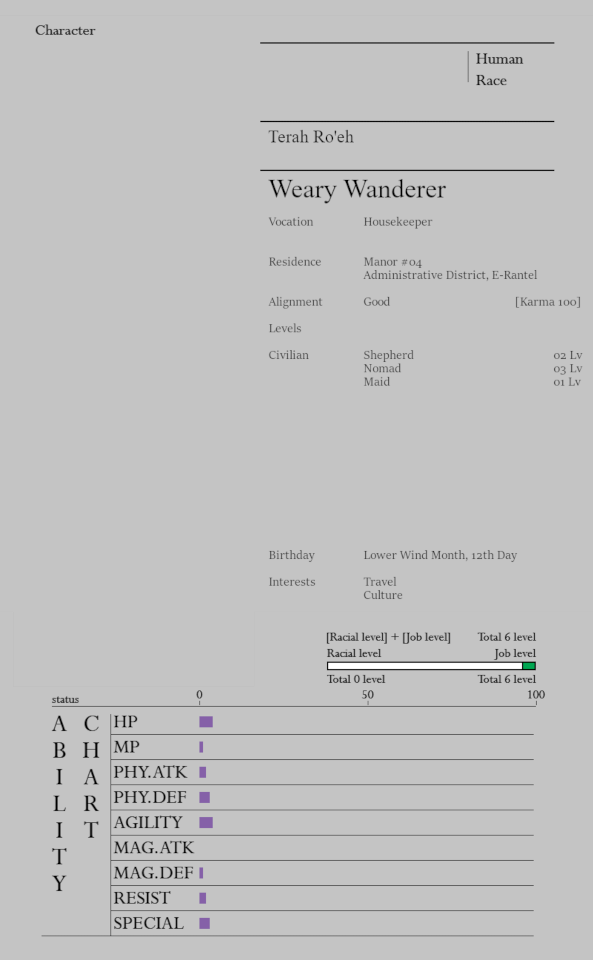
\includegraphics[width=1\linewidth]{V1 Birthright//images/8ugC7a1.png}
    \caption*{Terah Ro'eh Character Sheet}
\end{figure}


\section*{The Noble Household (Part II)}

Those women serving in domestic matters within a household – colloquially termed ‘maids’ – cover a wide range of specialized roles with varying degrees of importance and authority.

 

Housekeepers are managers over the majority of the women serving in these domestic tasks, reporting directly to the lady of the house. They are responsible for hiring, development and promotion of those working under them and the overall condition and appearance of the manor. It is a senior position in the household retinue, and a Housekeeper is usually served by junior members of the staff.

 

A Lady’s Maid is a direct attendant of the lady of the house. They assist in managing their mistress’ wardrobe and appearance, as well as see to their various personal needs. Like the Housekeeper, it is a senior position in the household retinue and does not normally see to menial tasks that junior positions are responsible for. Though a Lady’s Maid also reports directly to the lady of the house, the Housekeeper holds authority over the rest of the female staff, and indirectly outranks her. A Lady’s Maid is not to be confused with a Lady-in-Waiting: a companion of noble birth who serves in a similar capacity.

 

Those most closely associated with the common perception of maids are the junior staff, each performing specific duties in their part of the manor. Maids who work ‘upstairs’ attend to tasks in the private areas of the manor. Those who work ‘downstairs’ tend to the common areas of the manor, usually on the main floor or storage areas. The grades delineating their positions in the household hierarchy is usually dependent on the nature of the work itself – those assigned to the most menial tasks tend to be the least respected and subjected to the worst conditions.

 

It should be noted that maids performing kitchen duties do not report to the Housekeeper, but to the Cook.
\chapter{Ludmila Zahradnik}

According to the Elder-Lich-turned-clerk, it would take half an hour to process their request. Ludmila was directed to one of the alcoves to wait to be called upon. It had enough room to seat four people on its cushioned benches, with a magical glass lantern that cast its light over the polished wooden table. With a sound resembling a light grunt, Ludmila set all of her things down, pushing it towards the wall. She waited for Lady Shalltear to be seated before taking her place across the table from her.

 

“Do you think things will go well, my lady?” A shadow of doubt still played across Ludmila’s mind after she had submitted her requests, “It seemed a bit too easy.”

 

“The clerk submitted your documents to be processed,” Lady Shalltear shrugged. “There are not many layers of bureaucracy to get through…there should be someone that double checks your documents, then another who organizes the orders. Like I said earlier, these Elder Liches are newly trained, but they are eager to prove themselves useful in their service to His Majesty. It would consider any errors on its first official job absolutely unacceptable.”

 

“So you do know how things work,” Ludmila said.

 

“I know bits and pieces here and there,” Lady Shalltear admitted, “I’ve been…placed on standby for the last little while, so between ensuring my territory is secure and seeing to the realm's logistical needs, I've had a lot of free time on my hands. I wander the city and the realm, watch what goes on and sometimes I do some things for myself, but I would much rather be serving His Majesty directly in some way.”

 

Lady Shalltear seemed a bit sullen as she spoke, and her downcast manner made Ludmila frown. Once again, her liege acted in a way which seemed very out of place with the quality of the woman who had graciously taken Ludmila under her wing.

 

“Well, I for one am appreciative of your time on my behalf, my lady,” Ludmila said in an attempt to pick up her spirits, but she didn't think the gratitude of a relative nobody counted for much.

 

“Hmph, spare me the flattery,” Lady Shalltear rested her cheek in hand. “The Royal Court has been working hard to carry out His Majesty’s Will. In His infinite wisdom, He has given us the time to fulfill His wishes, but that time will be over sooner or later. We must present to Him a thriving realm, and we dare not disappoint Him. You are simply a means to that end.”

 

“Then what is His Majesty’s Will?” Ludmila asked.

 

“You were there yesterday, were you not?” Her liege answered, “What I declared to the people in the city are His wishes for the Sorcerous Kingdom.”

 

“But surely that can’t be all?”

 

There was a long pause between them. Lady Shalltear traced a circle over the surface of the table as she thought on what to say.

 

“Well…His Majesty is truly unfathomable,” she replied, “so it is only what we have discerned from both His stated intentions and His actions. He desires a realm where all peoples can thrive and prosper. A nation that can shine as a testament to His mercy, wisdom and glory to the rest of the world. Lord Ainz has the power to turn these territories into a blasted and barren wasteland, yet He chose to grant a swift and decisive end to those who would oppose Him and presented a hopeful future to His new subjects. As His loyal vassals, we cannot understand – in our eyes, the Humans of this realm are repaying grace with spite.”

 

Ludmila felt a pang as Lady Shalltear lamented the current state of affairs. To have one’s goodwill and effort go unappreciated and perhaps even scorned was not something anyone could feel pleased over.

 

“I assure you that is not the case, my lady,” she said reassuringly. “You might not trust the people of the city when they say so directly, but you should not let this sentiment fester in the Royal Court without confirming whether it is true or not. Admittedly, I have only been here a short while, and I do not know everything that goes on in the city, but not once have I heard anyone – not the nobles, nor the common folk – speak in ways that I would consider spurning His Majesty’s goodwill.”

 

Lady Shalltear watched her carefully as she spoke, yet somewhere along the way, her expression started to sour.

 

“Is something the matter, my lady?” Ludmila spoke carefully as a scowl began to form on the Vampire’s face.

 

“Then why?” The question was delivered in a low voice, a growl from a beast about to pounce on its prey.

 

“I-it’s because–” she stammered as she watched Lady Shalltear’s appearance shift, the ethereal visage of delicate beauty melting away, leaving only the menacing image of her true form.

 

“WHY?!” The Vampire’s voice had turned into a rasping, malevolent hiss, filling the alcove.

 

Ludmila was about to glance beyond the secluded space to see if anyone was watching, but the crimson glare flared and her will was forcefully wrested away from her before she even knew what was happening. Dozens of rows of needle-like teeth came close, and the tinge of blood filled the air.

 

“Tell me!” Lady Shalltear’s voice came out as a sibilant whisper that slithered into Ludmila’s mind, “Tell me the truth. Tell me why these Humans continue to defy the Will of Lord Ainz!”

 

“They are not defying His Majesty’s will,” Ludmila felt her own voice come out in response, flat and emotionless, “they are only scared. It is only fear.”

 

“This is a lie! A lie! Fear? What is there to fear? Are His precious words not enough for you? Do you believe it to be deception? Tell me, is it hate? Do you hate Him? He, who has granted His infinite mercy to you – to us?!”

 

As the questions broke over Ludmila one after another, Lady Shalltear’s voice rose as her words turned into accusations. A tear rolled down the pallid flesh of her cheek at the last as she howled at her.

 

“I would strike you all down for your insolence, if not for His order to stay my hand. Turning this entire world into a sea of boiling blood would not nearly be enough to pay for your scorn!”

 

“It is not a lie," Ludmila said. "It is not distrust; it is not hate. It is fear…and we are only Human.”

 

For long moments, Ludmila was pinned in place by the Vampire’s gaze. She watched as the image of Lady Shalltear’s beautiful form eventually returned, superimposed over her true appearance. As she pulled back from leaning over the table and settled into the cushions of her seat, Ludmila felt herself being released from her liege’s mental hold. Across from her, Lady Shalltear was drying her tears with a handkerchief that she had pulled from a pocket inside her bolero. Several minutes passed in silence, before Lady Shalltear spoke tentatively.

 

“I...I...was just thinking about my Lord’s wishes,” she said, twiddling the silken handkerchief in her fingers. “About how nothing ever seems to go in the right direction…and I lost myself. You will forgive me.”

 

“You are forgiven,” Ludmila replied in a flat, emotionless tone.

 

The fingers stopped and she looked up at Ludmila, squeezing her eyes shut tightly and opening them again as her eyelids fluttered and her slitted pupils dilated. Realization that Ludmila had imitated a charmed voice dawned over her face.

 

“That’s not funny!”

 

Lady Shalltear tried suppressing a laugh, but failed; the effort resulting in something halfway between a laugh and sob. She sniffed, then blew her nose loudly into her handkerchief. Ludmila waited quietly, attempting to reassert her usual mental state before speaking.

 

“When we spoke yesterday,” she said, “you expressed the state of the citizens before I could even share my thoughts on it. You always speak of your service to His Majesty fondly, and I don’t think anyone could question your devotion when they hear you. If I found something that inspired such conviction in me, I think I might become furious as well if something like this happened.”

 

“I swear…if you keep up with that unwavering coolheadedness of yours,” Lady Shalltear said, “you’ll turn into a Golem one day.”

 

“…is that even possible?”

 

“No. Not like that, anyways.”

 

Ludmila wondered if Lady Shalltear was trying to get back at her for her prank. The thought brought her back to what had occurred between them.

 

“That ability that you used just now…” She asked, “Is that what it feels like every time I use my own on Luzi?”

 

“What, are you trying to make me feel guilty?” Lady Shalltear made a face, “No, that was an ability that Vampires possess. Our power to charm others has to do with the supernatural nature of our race. Your abilities have to do with your own race: Humans have a social caste that specializes in administration and leadership; so your Nobles have abilities related to their role in Human society. Demiurge – one of the most intelligent of His Majesty’s servants – speculates that every race with a ruling caste will have their own classes along the same vein as your Human aristocracy. He also speculates that races that have become overly reliant on the abilities of their ruling class can be easily disrupted by eliminating them at opportune moments, or better yet – by taking control of them in some form and having them lead in a manner that suits our objectives.”

 

Ludmila felt that talking about usurping those in leadership while sitting in a government office seemed terribly wrong, so she steered the conversation in a different direction while nervously looking towards the reception counter.

 

“Still, telling people to do something and having them act as a result of an ability,” Ludmila mused. “Even Countess Jezne only seemed to be able to encourage the nobles around her to collect themselves...if that was even her ability at work. I still can’t tell whether one has been persuaded to act through normal means or through the use of an ability.”

 

“Yes, that’s something interesting I noticed as well,” Lady Shalltear said. “What you did was not just subtly influencing others, but reinforcing them and ordering them into action. This is something that those with Commander classes do, but as of yet, we haven’t encountered any other Nobles that have demonstrated active command abilities. We know that Commanders exist amongst Humans at large – Carne Village reportedly has a Farmer girl with the ability to do so, but this arose out of a decidedly strange set of circumstances. Since Humans appear to have many classes that are unfamiliar to us, I think you may have something along those lines.”

 

Ludmila already knew how she was going to reply – it had been under her consideration for a while now.

 

“There is something you said earlier: to think about what people notice that I never considered truly special. More than a few have mentioned nobles from the frontier as being…beyond the rest of their peers – that we were made differently, somehow. My maids said something along these lines shortly after we were first introduced and they entered my household.”

 

“Oh?” Lady Shalltear straightened in her seat, “This is a promising lead. What did they say, exactly?”

 

“Aemilia said that I could brave the city streets when none of the other nobles were capable of doing so,” Ludmila made an account of her memories, “even after said nobles had worked up the courage to try. That I appeared like a gallant warrior, ready to fight at any time. Countess Jezne said she had expectations of me, though she never elaborated on what she meant. Bohdan – the village priest in Warden’s Vale – remarked that I shared a similar trait with my ancestors: the willingness to face danger with a resolute will and he, too, told me that the people of the frontier were different than those of the interior. My parents said many things as well, but all noble parents seem to teach their children that they are superior in some way…I never really considered it seriously until now.”

 

“So is it true?” Lady Shalltear asked, “Everything that they said about you.”

 

Ludmila shifted uncomfortably in her seat: frontiersmen were not ones to brazenly advertise themselves, and she was no exception.

 

“I think so, yes,” she replied. “There’s so much more now that you’ve brought it to my attention. My brothers were much better fighters than the other noble scions when they practiced together, and they almost always stood at the centre of a crowd. I can feel that I am stronger than other people as well: I can run a bit faster, last a bit longer, carry more and fight better. My parents could outfight any of the Rangers and Fighters in the village, and during the Battle of Katze Plains, my lord father was able to keep his men from breaking…right until the end.”

 

Ludmila swallowed after the last of those words left her mouth. She wasn’t sure when she had decided her family was lost, and now she felt absolutely terrible hearing herself say as much.

 

“Hmm…this is a lot to think about.” Lady Shalltear said solemnly, “If all these claims can be proven to be true, then it will be a matter of grave importance.”

 

“Surely you cannot mean that, my lady,” Ludmila said incredulously. “With so many powerful servants at His Majesty’s disposal, it hardly seems to matter.”

 

“You’re correct that at your level it makes a negligible impact in combat as an individual,” Lady Shalltear agreed, “but a Commander placed over a company of powerful soldiers should still make them that much stronger. I would also be negligent in my duties to think that the world would conveniently present weak opponents forever. I need to speak to Demiurge about this – no, Momon would be the closest to an expert that we have. He was even right about you yesterday during the council meeting…just how much of this has he planned out, I wonder?”

 

“You will be taking your leave then, my lady?” Ludmila asked.

 

“No. You Humans have your inconvenient need for sleep, and we’ve still other things to do before your day is over.” Lady Shalltear looked to the reception area, from where a figure approached, “I believe your paperwork has gone through.”

 

An Elder Lich had appeared from the office behind the counter, circled around the reception desk, and was now purposely walking their way. Its tattered robes of black silk shimmered as it walked by the windows and it held a long, gnarled staff in its right hand. The end of the staff touched the ground in time with its steps, but Ludmila could hear neither the tapping noise that should have accompanied the action, nor the sound of the Elder Lich’s footfalls.

 

It came to stand a few metres away, bowing to Lady Shalltear, then looked to Ludmila. It had the same stained strips of cloth lined with strange lettering like the other Elder Liches at the counter. In addition, it held a large, leather-bound tome pressed to its chest.

 

“Is it saying something, my lady?” Ludmila frowned, “I was watching it approach, but I did not hear anything at all.”

 

“Oh, that’s right.”

 

Lady Shalltear motioned for the Elder Lich to step forward. After a single stride, its footsteps could be heard – as could the sound of its staff tapping on the floor.

 

“The Humans that constructed this city are quite adept at building spaces for large numbers of citizens in close proximity,” her liege said. “These alcoves were designed to provide privacy without the need to construct additional rooms. We’ve revisited many of these concepts when we occupied the city and created additional security measures. We decided for a Silence spell to be maintained for these alcoves so that the office’s clients can discuss their personal business privately within.”

 

“The other nobles should be pleased with this consideration once they become accustomed to life in the city, my lady.” She looked up to the Elder Lich that was now standing beside the table, “So…were there any problems with my submitted requests?”

 

“No outstanding issues were identified,” it replied, and Ludmila let out a relieved sigh.

 

The Elder Lich had a markedly different voice than the one they had spoken to at the counter. It still had something of an abrasive and dry rasp, but the tone was distinctly female.

 

“Your request is being seen to,” it informed her, “and will be arriving shortly outside. This one has been ordered by the Guardian Overseer to accompany Baroness Zahradnik to her territory as an attaché.”

 

“An attaché?” Lady Shalltear peered suspiciously at the Elder Lich, “why would Albedo suddenly want to stick her big nose into something she didn’t want anything to do with just yesterday?”

 

“Lady Albedo has deemed it to be the most efficient manner by which to fine tune various mechanisms of administration and labour in their associated fields.” The Elder Lich replied dispassionately, “This has been mandated as standard practice when information is insufficient to publish suitable manuals.”

 

“Ugh, did she train you to speak like that too?” Lady Shalltear complained in a long-suffering tone, “The last thing I want to hear is hundreds of Elder Liches parroting that insufferable bi–ahem–the Guardian Overseer.”

 

The Elder Lich gave no response, which in turn appeared to worsen Lady Shalltear’s disposition.

 

“Where will the units from the request be delivered?” Ludmila hurriedly filled in the silence, “Will I be able to review them before they are deployed?”

 

“They are currently en route to the main avenue,” the Elder Lich answered. “You may review them in front of the civil office.”

 

As if on cue, Aemilia appeared in Ludmila’s line of sight, standing over five metres behind the Elder Lich. Her lips were moving as she made fretful motions with her hands, but the enchantment preventing sound from crossing the threshold of the alcove stopped the maid’s words from reaching her. Ludmila rose from her seat, stepping past the Elder Lich to leave the alcove.

 

“–ounded by Undead, my lady! Thousands of them!”

 

Aemilia’s panicked words met her as she stepped out of the alcove. Her auburn hair was jostled as she bounced anxiously on the balls of her feet.

 

“What do we do?” She said worriedly, “Are we under attack?”

 

Ludmila placed her hand on the maid’s shoulder to still her as she turned her head to look towards the window. The angle was poor, so she ended up walking out of the office entrance to take a look from the top of the stairs. Arrayed below were her requested workforce, but rather than a loose collection of various labourers, they were neatly organized like a company of professional soldiers.

 

On the road nearest to the sidewalk were forty Bone Vultures, arranged in a rectangle ten wide and four deep. Directly adjacent to their formation was another consisting of twenty Undead Beasts in the form of Boars: they were set five wide and four deep. Behind their lines were one hundred Skeletons armed with round shields and short spears that glistened when breaks in the mostly overcast skies allowed the sun to shine through. Like the Undead Beasts, they were arranged in groups of twenty. At the corner of each of the Skeleton formations, a Death Knight stood where a sergeant would normally be. The Death Knights still held their massive tower shields, but their blades were sheathed. Their weapon hands instead gripped tall banners upon which the vermillion standard of the Sorcerous Kingdom flew proudly in the spring breeze.

 

Ludmila supposed that if it were a company, then all they lacked was a captain. She stepped down to take a closer look, and as she arrived at the bottom of the stairs, the avenue was filled with a singular noise as the entire group stood to attention. Lady Shalltear appeared at Ludmila’s arm with her dark parasol open over her shoulder, speaking over the stiff breeze that scattered the spring blossoms into the air around them.

 

“Are they to your liking?” She asked her.

 

“The numbers check out, my lady,” Ludmila replied. “However, any spectators would think that I am about to go forth to conquer my enemies rather than conquering unruly fields.”

 

“You have enemies?” Lady Shalltear raised an eyebrow, “That’s hard to imagine considering how unflappable you seem to be.”

 

“Well, there are types that we are not particularly fond of, but not in the sense that most would consider enemies to be.” Ludmila thought to the wariness that her father held for Count Fassett, “Being Frontier Nobles, House Zahradnik stood apart from the squabbling that occurs in the interior. Our enemies have always ever been those that would infringe upon and act unlawfully within the realm of our liege.”

 

“If it had been any other of your kind standing here saying that,” Lady Shalltear said, “those words would have felt like lip service, I think.”

 

“Did I unconsciously use my ability on you, my lady?” Ludmila made to apologize.

 

“I doubt it,” her liege smiled slightly for some reason. “Undead are immune to mind-affecting spells and abilities.”
\chapter{Ludmila Zahradnik}

Lady Shalltear’s Vampire Brides, Aemilia and the Elder Lich joined them shortly after; each of the three attendants carrying a portion of the books and files that remained after Ludmila finished submitting her forms. Arranged before her was the manifestation of those forms, and Ludmila was now mentally going through the checklist of things that she wanted to have taken care of before the day was over.

 

The applications that she had filled were meant to provide only raw labour, so the fact that many of the Undead standing in front of her were armed was unexpected. Unfortunately, being armed did not really help with the task she had requisitioned them for. It was up to the applicant leasing the Undead labour to provide the appropriate equipment, though there were a few recommendations that came with them in the provided almanacs. In hindsight, procuring the Undead labour was probably the easier part of what she had to do: it was the exact opposite of what she had originally expected to go through to find new tenants. Though she would still need to find tenants to direct the Undead Labour, the number required was drastically reduced compared to what would have been required before. Ludmila thought that she could at least get things started while she waited for them, and see how things worked for herself. She turned to address Aemilia.

 

“Luzi, take these things back to the guest house,” she instructed her maid. “Actually, hand me the blue folder first – I’ll be needing that.”

 

“Yes, my lady,” Aemilia said as she handed over what had been requested.

 

“I hope you don’t mind my borrowing your servants, Lady Shalltear,” Ludmila said.

 

“It’s not a problem,” Lady Shalltear replied. “We’re trying to produce results as quickly as possible here.”

 

Ludmila turned to the Death Knights that had accompanied them.

 

“Escort Luzi back to the guest house,” she told the one standing on her left, “return with her when she has completed her task.”

 

Aemilia, who had already started to walk back to the house, overheard that a Death Knight would be coming with her. She darted along the road with the Vampire Brides, walking faster and faster over the cobblestones, but the Death Knight slowly closed in on them despite her efforts.

 

“I hope no one gets the wrong idea seeing that,” Ludmila remarked as she watched the Death Knight chase the women up the street.

 

“I thought the goal was to assuage the fears of the citizens, not feed them.”

 

Ludmila frowned and looked down towards Lady Shalltear, but the Vampire only looked on innocently. Ludmila turned to the Elder Lich.

 

“Well, I suppose we should get on with the next order of business,” she said. “Will these labourers stay here, or is there somewhere that they can assemble and wait for their equipment?”

 

“They were instructed to present themselves for inspection in front of the Civil Office,” the Elder Lich answered, “they are under the leaseholder’s authority upon delivery.”

 

Ludmila looked around absently as she thought of a place to have them wait – leaving them in the main avenue of the central district was probably something that would disrupt traffic if the city was even slightly busy.

 

“Are they permitted transit through the city on their own?” Ludmila asked.

 

“They will not be intercepted if they traverse the city in a non-disruptive manner,” the Elder Lich answered.

 

“Alright then…” She turned to her new labourers, “Head to the Military District, using the main roads. Assemble at the first available mustering field to the west of the south gate and await me there.”

 

The Bone Vultures all took wing at once, while the other groups of Undead marched away in formation. Ludmila watched with some satisfaction as the formation filed off under her orders.

 

“That was interesting,” Lady Shalltear noted from beside her. “You didn’t even raise your voice to issue your instructions, but they all heard you over the wind. Considering that you just realized you had these powers...when did you learn how to do that?”

 

“Just then, my lady.” Ludmila’s voice was a bit bemused as she answered, “I was actually going to raise my voice like those famous captains and generals in the tales that minstrels tell, but when I started speaking, I noticed that even the ones all the way in the back that shouldn’t have heard me had already reacted. So I just spoke normally. In regular circumstances, they should not have heard me, but this ability carried my voice to everyone.”

 

“Did you know if they would arrive at their destination?” Lady Shalltear said.

 

“Er…no?” Ludmila looked towards the receding labourers in alarm, “Wait, they won’t?”

 

“They will, in this case,” Lady Shalltear replied. “As long as they receive their orders, they will perform according to your intent…as long as it is something that they themselves are able to manage without more precise direction. In the worst case, the Death Knights with them will rally any lost Skeletons. You will probably need to show these labourers how to do some uncommon things at some point, since your territory seems to produce goods that are not commonly cultivated in Re-Estize.”

 

Ludmila breathed a sigh of relief. The last thing she needed was to have inadvertently commanded her newly acquired workforce to rampage through the city on the way to their destination.

 

“Well then,” she said. “I need to find where my goods have disappeared to now…”

 

“What happened to them?”

 

“Before I left Warden’s Vale, Momon threw everything into a hole much like the one that you used yesterday evening.”

 

“Ah, yes, that was me. Aura and Mare had quite the time catching all those things that suddenly came flying through,” Lady Shalltear smiled at the recollection. "Your goods are in the government warehouses; let’s be on our way.”

 

Lady Shalltear turned in the direction of the Royal Villa and walked off. Ludmila followed, and the Elder Lich followed after Ludmila. The day had brightened considerably since the morning, with the overcast skies breaking up to reveal the azure heights beyond. A brisk wind was sending the clouds southwards rapidly; she wondered if the rain of the previous night would arrive as snow in Warden’s Vale.

 

They continued around the Royal Villa and past the gazebo that was used as the location to teleport in and out of. The entrance to the city stores was a fortified and guarded gate tucked away on one side of the central district, where a ramp led down to the vast warehouses had been carved deep into the hill below. The city had furnished it with magical devices that enchanted the entire space with a Preservation effect, which would keep the tremendous volume of siege provisions stored within from spoiling. They passed between the two Death Knights standing guard at the top of the large ramp that led down into the cavernous areas below, steps echoing lightly off of the tunnel-like passage.

 

After two turns, most of the light had been swallowed in darkness, and Ludmila found herself looking at row upon row of shelves that reached all the way to the ceiling, which was perhaps five metres above her head. They were supposed to be filled with the supplies that had been meant for the armies of Re-Estize, but after scanning their contents, she saw that the nearest portion of the warehouse was already being emptied and there were many bare spaces. After passing several aisles, Lady Shalltear stopped and turned to face an aisle to her right.

 

“The things on the bottom shelf there should be yours,” she pointed down the way a bit, “make sure nothing has…wandered off.”

 

Ludmila stepped towards where Lady Shalltear was pointing and quickly located the shelf that appeared to have the goods from the warehouse in Warden’s vale. They had taken up a significant portion of the storage space in her home village, but here they only occupied perhaps one third of the bottom shelf of a small fraction of the city warehouse. She felt rather tiny as she checked what she saw against one of the documents in the blue file folder to ensure that everything was in order.

 

“It looks like everything is here, my lady,” Ludmila called out, “are there problems with theft down here? The security in the city seems overwhelming.”

 

“I was just making sure,” Lady Shalltear said. “There are no issues with thieves, but samples are sometimes taken for analysis if we find something that might be interesting or different. What do you plan on doing with all this?”

 

“I need to have it loaded onto a wagon, and then search for someone that is available and willing to purchase these goods.”

 

“Well none of the ones in the warehouse are being used, so it shouldn’t be an issue. You,” Lady Shalltear addressed the Elder Lich, “submit a request for a wagon from here on behalf of Lady Zahradnik. We’ll pick you up at the civil office on the way out.”

 

The Elder Lich bowed silently, and walked away towards the entrance.

 

“I was not aware that they could do that, my lady,” Ludmila said as the tapping of its staff receded into the distance.

 

“Well, it’s supposed to be your administrative attaché, is it not? I’m pretty sure you Humans do the same thing – sending others that function under your authority.”

 

“That is correct, my lady,” Ludmila admitted. “I guess my family has just always done most things directly.”

 

The tread of a Death Knight and the light of a lantern coming from the entrance drew their attention. The four that had left to drop off Ludmila’s files had returned.

 

“Did you run into any trouble?” Ludmila looked between the members of the group as they arrived, “Actually, how did you even find us? I do not recall mentioning where we would be headed.”

 

“No, my lady,” Aemilia said, “Lady Shalltear’s attendants appeared to know where you went after we parted. Mrs. Ro’eh asked if you would be having lunch at the house.”

 

The maid’s question reminded Ludmila of the wholly inadequate breakfast from the morning.

 

“Hmm…what is she preparing?” She asked.

 

“She was not aware of any itinerary, my lady – only that you would be out for most of the day,” Aemilia replied, “so it’s a meal that can be packed if necessary.”

 

“That will be fine,” Ludmila nodded. “Head back to the house and let her know. While you are there, find my scarf and shawl and bring it with lunch – this wind keeps getting stronger. Wait for us in front of the civil office; you should see the Elder Lich waiting for us there as well.”

 

Aemilia’s head nodded at each instruction. When it seemed that there would be nothing more forthcoming, she curtseyed before them and turned to leave.

 

“Continue escorting Luzi.”

 

Ludmila told the Death Knight to maintain its orders, and Aemilia looked at her like she was about to cry.

 

“Do not run away from your escort this time,” Ludmila instructed her maid, “it looked like you were about to be murdered on the street just now.”

 

Aemilia’s mouth worked silently as she looked back and forth between her mistress and the Death Knight, her expression asking how she ended up being in the wrong somehow. When it was clear that she would receive no consolation, she sighed and slowly walked off.

 

“Despite claiming to be used to doing things directly,” Lady Shalltear noted, “you certainly don’t seem to mind running your new staff back and forth.”

 

“Luzi is aspiring to be my lady’s maid,” Ludmila explained, “but my household currently does not have a page, and the footmen would scare everyone else witless. She should understand this as well as I. Besides, her visibility in the streets in the company of the Death Knight contributes to the idea of safety that we are trying to promote amongst the citizens here, yes?”

 

“I see. Well,” Lady Shalltear looked over to direct her Vampire Brides, “let’s get these things off the shelf and ready to load on the wagon.”

 

From the depths of the warehouse, the sound of hooves on stone echoed through the aisles. As her inventory was arranged near the path that ran through the warehouse by Lady Shalltear’s attendants, a wagon drawn by a skeletal horse turned the far corner. Lurid light shone from within its bony frame, which was embraced with sickly yellow-green fog that shimmered and rippled like living flesh as it trotted forward.

 

The wagon appeared to have no driver, yet it rolled smoothly to a stop in front of them. The Vampire Brides immediately began to place the various articles onto the bed of the wagon in an orderly fashion. Taking in the details of the skeletal horse, Ludmila turned her head towards Lady Shalltear.

 

“Is this an Undead Beast as well?” She asked, “It seems quite different from the ones that you showed me earlier.”

 

“This is a Soul Eater,” Lady Shalltear replied. “They are level forty, so substantially more powerful than a simple Undead Beast.”

 

“This…horse is more powerful than a Death Knight?”

 

“They have very different sets of traits and abilities which makes them useful for different things, but yes: in rough terms, they are.”

 

Ludmila envisioned a teamster driving a cart pulled by beings that could destroy a city. What would happen if there was an accident?

 

“What happens if the cart breaks, or if there is some sort of mishap?”

 

“Hmm…that hasn’t happened yet,” Lady Shalltear tilted her head in thought, “but it’s strong enough to forcefully drag a broken cart loaded with goods around. I’m not sure if everything will stay on the wagon in that situation though; the wagon itself might break apart.”

 

Lady Shalltear hopped onto the driver’s bench as the Vampire Brides loaded the last of the goods. The two attendants took their seats at the back of the wagon bed, their pale legs dangling off the edge. Ludmila pulled herself onto the driver’s seat beside Lady Shalltear. The Soul Eater turned its head to look at her with a glowing eye socket.

 

“Let us pick up the others at the civil office first,” Ludmila said.

 

The Soul Eater turned its head back and began plodding forward. Ludmila looked over her goods worriedly as the wagon rolled up the ramp, but the shallow incline leading out of the warehouse was not steep enough to cause anything to slide out of the back of a loaded wagon bed. She watched the skeletal horse as it made its way up – pulling a freight wagon was something that normally required large teams of horses, yet this single Undead being did so effortlessly.

 

They found that the clouds had completely broken since they entered the underground warehouse, and the warmth of the sun was rapidly turning the day pleasant. Free of the need to carefully maneuver through the tight turns leading out of the warehouse, the Soul Eater picked its pace up to a brisk trot, and the noise of its hooves on the cobblestones made it seem like they were being pulled along by a regular horse – at least until one looked at the horse itself.

 

It took all of two minutes to reach their destination as they circled around the district, finally slowing to pull up in front of the civil office. The trio waiting by the stairs turned their heads at the sound of the wagon’s approach. Aemilia visibly jumped at the sight of the Soul Eater, and she seemed on the verge of panic until her eyes found Ludmila sitting in the front seat with Lady Shalltear. She spotted the other attendants sitting in the back of the wagon and circled around, handing her lunch basket to one of the Vampire Brides so she could pull herself up to join them.

 

Ludmila took a deep breath and released it in anticipation of what was to come. So far her day had been relatively straightforward with the help of Lady Shalltear and the smooth workings of the new administration. It had all been completed within a single morning: so quickly that the next group of tasks were already upon her before she could fully think through what needed to be done.

 

“Time for the annoying part,” she muttered to herself.
\chapter{Ludmila Zahradnik}

“You’ve been progressing steadily thus far,” Lady Shalltear picked up on Ludmila’s soft mutter, “why would the next part present any difficulties?”

 

“The next part involves finding the right people out of all of the citizens that are hiding in their homes,” Ludmila returned to her usual, clear voice, “and I am not quite sure how to accomplish this, my lady. Frontier Nobles are nobles, but we only share some very basic similarities with the nobles of the interior. You mentioned a little while ago about how you believe you are only good for fighting, but I am in something of the same situation as well. I have been trained in all of the things required to carry out House Zahradnik’s duties in defending the border – this would include logistics, organizing and leading armed patrols, as well as managing our small fief, but my skills in administration and commerce are nowhere near as substantial as someone like Baroness Corelyn. Our house does not have much in the way of connections, either.”

 

“Well what did you do last year, then?” Lady Shalltear asked.

 

“Our goods were sold to a wholesaler,” Ludmila answered, “merchants who have both the capital and storage to take in large quantities of goods and bide their time to turn a profit meeting the demands of the markets. That way, we would be able to return to our duties on the border within a couple of weeks, after dealing with some other noble functions. However, if the city is like this, not only will it be difficult to find such a merchant, but the markets will have slowed to nothing as well and the prices for everything may not be as projected.”

 

“So you have to ride around the entire city until you find someone?” Lady Shalltear frowned.

 

“Perhaps…perhaps not.” Ludmila turned to the Elder Lich, “Are there any markets that are still active in the city?”

 

“As of this morning, no open market areas have been reported in the city,” the Elder Lich replied. “Emergency supplies are currently being distributed by Lady Shalltear Bloodfallen and her staff in the interim.”

 

“What about guilds?”

 

“The Adventurer Guild and Mage Guild are maintaining limited operations.”

 

“How about the Merchant Guild?”

 

“There has been no reported activity from the Merchant Guild or any of its associated Trade Guilds in the past week.”

 

Ludmila bit her lip lightly as she thought about what she could do.

 

“How does the city procure goods when there is no commerce?” She asked.

 

The Elder Lich remained silent. Its fingers lightly tapped the leather-bound book that it held to its chest while it pondered her question. Lady Shalltear spoke, filling in for the perplexed attaché.

 

“The short answer is that we’re not, currently,” she said. “The government warehouse is slowly being depleted over time – you estimated that they would last one year, while the Guardian Overseer’s estimates are closer to two if rationing measures are enforced immediately. She expressed great confidence that E-Rantel would not need to resort to such a policy initially, but with the lack of progress in the past week I believe that she is beginning to consider it as an option.”

 

Ludmila grimaced. The siege-like nature of their situation felt ever more real with the idea that the people might begin to see their necessities limited.

 

“Will the city purchase goods while the markets are closed, my lady?”

 

“The Sorcerous Kingdom guarantees a minimum rate for basic materials,” Lady Shalltear said. “But...they would most likely not be favourable compared to regular market prices. The merchant I spoke of yesterday shouted ‘ridiculous!’ and stormed off, leaving Sebas standing alone in the street with only his good intentions to keep him company.”

 

“How was he able to trade in the city then?” Ludmila asked.

 

“I don’t think he did. The following council meeting, it was reported that he spent the day running all around the city’s markets and guilds with no apparent success. He left the city the next morning.”

 

Ludmila exhaled sharply. She had hoped that information from the lively merchant whom Lady Shalltear had mentioned would lead to a solution to her conundrum as well. With one avenue closed, she decided to pursue another, turning to the Elder Lich once more.

 

“Do you know where the nobles currently residing in the city are housed?”

 

The Elder Lich nodded silently.

 

“We will stop by the nobles’ clubhouse first, then,” Ludmila decided. “After that, we can find the remaining nobles that were not present there – the ones in the city should be in their respective manors here since they are supposedly too frightened to move around much more than that.”

 

As the wagon rolled forward, the two Death Knights fell in line to either side of the Wagon. The Elder Lich kept pace on the road at Ludmila’s side of the front seat. Lady Shalltear looked up at her from the side.

 

“You have an idea?”

 

“Perhaps, my lady,” Ludmila said. “My family was not as well-connected as the other nobles but, since everyone else here is staying put and not doing anything, I was thinking that we might be able to make use of their connections in exchange for a finder’s fee or perhaps a future favour. That is our best chance now, I think.”

 

It was not long until the wagon pulled up in front of the clubhouse. The ornate building did not show any signs of being occupied from the outside, though this was also the case for the previous evening.

 

“Luzi, come with me,” she called to her maid sitting behind. “Excuse us while we check if anyone is here first, my lady.”

 

Ludmila stepped down from the wagon as Lady Shalltear lazily waved her away. Aemilia joined her, stepping ahead to open the doors. They were greeted by an empty reception desk, and the lounge area was vacant as well. There were no odours of food or beverage in the air and the furniture lay pristine and undisturbed. Aemilia went around the halls, returning after a few minutes and shaking her head as she looked towards her.

 

“Alright,” Ludmila said, “I guess we will have to visit each of them in turn, then.”

 

After they returned to the wagon, she spoke with her attaché.

 

“I need to know where all the nobles in the city are staying – beginning with Baroness Clara Odilia Dale Corelyn.”

 

“Baroness Corelyn resides at guest house number eighteen,” the attaché replied almost immediately.

 

“Take us there,” she instructed the Soul Eater, “find a corner out of sight of the main entrance to stop, however. If the residents are still fearful, then we should keep their fears out of sight for the time being.”

 

The wagon rolled forward again with its small entourage.

 

Not half a minute had passed when the Soul Eater stopped in the service lane that ran along the wall, behind the outer ring of manors which circled the district. Ludmila stepped off of the wagon again, remaining still while Aemilia checked over her appearance. Lady Shalltear came around with her attendants, watching the maid as she worked to fix any flaws in Ludmila’s outfit.

 

“Have you considered getting enchanted equipment?” Lady Shalltear idly spoke as she observed their activity.

 

Ludmila turned her head at the question, trying to remain stationary for her maid.

 

“You mean arms and armour, my lady?”

 

Magical equipment was far beyond the means of her family, whose meagre fief existed only a little beyond subsistence. The outfit that she currently wore was all that consisted of her formal wardrobe, and even that had been the product of the better part of a year’s worth of hard work; it had required her to sacrifice other things in order to be able to afford it.

 

“Just daily clothing, in this case,” Lady Shalltear said. “Enchanted items will adjust to fit themselves perfectly to their wearer. They’ll also restore themselves to form unless they completely run out of durability, so you don’t even have to worry about the sort of thing you’re doing right now.”

 

Aemilia froze upon hearing this; her hands stopped partway while moving to fix a crease in Ludmila’s skirts.

 

“Is it normal to have magical clothing in your demesne?” Ludmila asked, “Re-Estize has little in the way of magical items. Most of them belong to Adventurers and mages, or are heirlooms of powerful noble houses. What people more commonly see are tools that help with daily life, like magical faucets or the lighting in the city streets.”

 

“It is. Even the lowest maids have enchanted uniforms, so there is no great fuss concerning maintenance. Nearly my entire wardrobe is enchanted to various degrees,” Lady Shalltear’s voice took on a rare proud note. “Perhaps one day, after you’re successful in your task, I’ll display a few pieces for you.”

 

“I have never seen enchanted clothing before, my lady, so that would be wonderful. I believe Luzi would be very much interested as well.”

 

The maid’s hands started working again. A minute passed before she stepped away, indicating that they were ready to move. Ludmila took the blue folder that lay on her wagon seat, and together they made their way around the guest house to the front. The Soul Eater, Elder Lich, and the Death Knights remained in the service lane, under the shadow of the wall.

 

Like all of the other manors in the district aside from her own, there was no one stationed to guard the entrance. The manor itself was styled in a similar appearance to all the other guest houses, though there were a few differences in its structure. Aemilia walked ahead to pull the chain for the doorbell and returned to stand behind Ludmila a few metres away from the entrance.

 

She heard movement coming from inside, but it was a long time before they heard someone walk up to the door. There was the brief sound of a lock tumbling before the entrance opened a sliver, and an almond-shaped eye peeked out. The eye looked from person to person until she recognized Ludmila standing amongst the group.

 

“Ludmila?” She said suspiciously, “This is not some sort of trick, is it?”

 

“We just saw each other yesterday Clara,” Ludmila replied, “why would this be a trick?”

 

There was a short pause as the fearful noblewoman examined her face, followed by a relieved breath as she visibly relaxed and fully opened the door. She was in a simple dress of pastel yellow, and she seemed well enough beyond her nervous countenance.

 

“Ever since Count Fassett,” she explained, “every time one of us goes to have an audience with the Royal Court, the rest wonder if they will ever return.”

 

“Have other nobles disappeared like this?” Ludmila’s eyebrow rose.

 

“At least one other that I know of,” Clara nodded, “then a little while ago, Baron Hamel was looking out of his window and started shouting about how some poor women were being run down in the street by the Undead. I could not even bear the thought, never mind look out to see. When the doorbell sounded, I thought it was the end for us.”

 

Baron Hamel? Ludmila tried attaching a face to the name, but came up short. However, she spotted the face of the boy she had left in the clubhouse the previous evening poking his head around the corner of the corridor further within the manor.

 

“Clara,” now it was Ludmila’s turn to be suspicious, “why is Baron Hamel in your manor?”

 

Clara noticed Ludmila looking past her shoulder and quickly turned her head to look behind her as the mop of sandy blond hair disappeared back around the corner.

 

“That’s…erm, the Baron has taken up residence in the neighboring manor, and we have neighboring fiefs as well. We already knew each other from before, and he wanted to stay over because he was scared to be alone.”

 

“I see,” Ludmila’s voice was flat.

 

“Nothing untoward has happened!” Clara’s amethyst eyes looked at her innocently, “It is just comforting to be with others with everything that has gone on recently. Besides, we followers of The Six have our own ways, yes?”

 

Ludmila supposed that Clara was correct: as followers of The Six, they had their own approach to selecting consorts. Still, harmful rumors might come out of it.

 

“What of your servants?”

 

“We do not have any! All the ones that were offered by the city were not in a state to work at all.” Clara laughed nervously, “Housework has been quite the adventure–wait, how do you have servants out and about?”

 

“They just needed a bit of confidence, I think.” Ludmila replied, “You should try and encourage them some time.”

 

Lady Corelyn gave her a strange look, not understanding the meaning of her words.

 

“Also one of the women with the Death Knight was probably my maid Luzi here,” Ludmila continued, “I sent her on a few errands with an escort.”

 

Clara’s mouth fell open.

 

“Y-you command these Undead now?” She asked.

 

“The Death Knights are on loan from His Majesty as footmen for my household,” Ludmila answered. “They are remarkably competent, actually.”

 

The fearful expression appeared on Clara’s face again and she looked all around, as if expecting Undead to be hiding around every corner. Ludmila stood to the side, allowing her a clear view of the street in front of her home. She calmed down again after seeing that there were no horrors lurking about.

 

Lady Shalltear lightly cleared her throat, and Ludmila proceeded to the matter at hand.

 

“I have come on official business, however,” she said. “Do you have some time to spare?”

 

“Oh, of course,” Clara’s eyes shifted over to Lady Shalltear, then back to Ludmila, “but who is this beautiful girl?”

 

Ludmila straightened, realizing that she had been rude to not introduce her liege first.

 

“Apologies for my rudeness in not introducing her beforehand,” Ludmila turned to present Lady Shalltear, “this is Lady Shalltear Bloodfallen, Minister of Transportation.”

 

Clara’s mouth was agape again.

 

“A-a Royal Councilor? Here?!” She immediately dropped into a deep curtsey, “Welcome to my residence, Lady Minister. Baroness Clara Odilia Dale Corelyn, at your service.”

 

“You have never seen Lady Shalltear before?” Ludmila asked curiously, “I thought all of the other nobles had an audience with the Royal Court upon their arrival in the city.”

 

“She might have been there, I-I am not sure,” beads of sweat formed on Clara’s brow. “There were…others there, and I was scared witless. They sent me away and I can barely remember anything about the audience. A-anyways, I am being rude. Allow me to entertain you in the parlour; we have some refreshments…biscuits that were delivered earlier today. We have water as well, as long as you do not mind the charred flavour.”

 

“We are in a bit of a hurry, actually,” Ludmila said as she glanced sidelong to Lady Shalltear, “I need to borrow your merchant contacts in the city.”

 

“Merchants? I don’t think your demesne uses the same merchants as ours does, does it?”

 

Clara was right; the territories on the gentle slopes of the Riverlands cultivated vast vineyards and orchards which went into the desserts, jams and liquors produced in the territory.

 

“Anything is fine at this point,” Ludmila said. “Even if they cannot help directly, they might know someone who can. How about blacksmiths – toolmakers and the like?”

 

“We have a village blacksmith that does nearly everything,” Clara replied. “Merchants passing on the highway to and from the Theocracy sell us raw materials and everything else, usually.”

 

After they received what information Baroness Corelyn could provide, Ludmila thanked her and they started walking back to the wagon.

 

“Writing with a stick of charcoal seems a bit inconvenient,” Lady Shalltear remarked as Ludmila wiped her hands on a handkerchief.

 

“Carrying an ink bottle around would be a mess waiting to happen, my lady,” Ludmila said as she settled back on the driver’s bench.

 

“I can lend you a pen, if you’d like,” Lady Shalltear held out her hand, and an elegant-looking instrument appeared in her fingers, “you're going to have charcoal stains everywhere by the time we’ve gotten all the information we need.”

 

“This is…a fountain pen?” Ludmila tried writing with it, and her letters came out smoothly. “Thank you Lady Shalltear…or is it Lady Bloodfallen?”

 

“My vassals usually address me as Lady Shalltear, so what you’ve been using is acceptable.”

 

The next house they came to was occupied by Count Völkchenheim and, to Ludmila’s surprise, the door opened shortly after they came calling. A tall, middle-aged man with a rough appearance appeared in the doorway, holding a long bronze candlestick in one hand. Something about the image he projected tugged at the edge of Ludmila’s recognition.

 

“Oya?” After noticing that it was not some monster that had come to the door, he placed the candlestick aside and his face brightened, “To what does House Völkchenheim owe the pleasure of such beautiful young ladies today?”

 

“Count Völkchenheim?” Ludmila asked while still attempting to place his appearance.

 

“Ah, no,” the man hastily denied the appellation, “I am Andrei, a retainer of the Count – currently serving as his valet.”

 

His movements and mannerisms finally came together in Ludmila’s mind.

 

“A Ranger?”

 

“Why yes, young miss,” he replied with some surprise, “how did you know?”

 

Ludmila felt a bit of a twinge. Völkchenheim County was not a frontier territory, but they had been forced to take up arms to defend themselves as the frontier territories that were supposed to be holding the wilderness at bay slowly collapsed. Demihuman raids on their territory were not severe, due to their distance to the border ranges, but it was still something of an unasked-for burden.

 

“I am Baroness Ludmila Zahradnik,” she introduced herself then motioned to her right, “this is Lady Shalltear Bloodfallen, Minister of Transportation. We are here to speak with Count Völkchenheim.”

 

Andrei’s face paled as the titles rolled out of Ludmila’s mouth.

 

“Forgive my rudeness, Lady Bloodfallen, Lady Zahradnik,” he hurriedly bowed, his voice rising in apology as he bent at nearly a perpendicular angle. “I will call for the Count–please, come in and take a seat in the patio garden…”

 

His speech slowed as he looked to be deciding whether he should be seating the Count’s visitors, informing the Count of his guests, or dividing himself in half to accomplish both tasks at once.

 

“We won’t be long – we just require some information from Count Völkchenheim,” Ludmila spoke to eliminate his indecision. “It will be fine for us to wait here.”

 

He gave them one last, conflicted look before leaving the doorway behind and disappearing around a corner. They heard him shouting for the Count, then he seemed to cut himself off realizing that he was shouting for a noble in the presence of other nobles.

 

“Well, he certainly seems quite different,” Lady Shalltear mused.

 

“He carries himself like a frontiersman,” Ludmila said, “To be honest with you, I am more used to that sort of conduct than I am this whole dance of etiquette that the inner nobles conduct.”

 

“Perhaps you should act more like yourself then?” Her liege suggested, “There’s no need to put on airs with me.”

 

“I am acting like myself,” Ludmila replied, “at least how I act in an urban, public setting. The villagers I am used to are the ones that act like him…also my brothers…and my father.”

 

“Are you saying you’re the only person in your entire Barony that acts like this?”

 

“Well, yes,” Ludmila paused for a moment. “Though my mother did so as well; everyone says I take after her. Even though we were a remote border territory, she always behaved in a manner that suggested we were more than that and everyone around her was influenced as a result. Thanks to you, my lady, I understand why she did this now.”

 

“So when you’re out in your own territory, you speak more like this fellow?”

 

“Not exactly, my lady,” Ludmila replied. “Well, perhaps more informally. My conduct, however, would be unacceptable in the city according to Luzi here.”

 

The maid reacted to being named, but stayed silent. There was a thumping of heavy footsteps as someone came down the stairs, followed by a shadow in the light of the courtyard inside. A young man appeared in the hall, looking very much like he had rushed to dress and groom himself. Somewhat winded, he came forward, but stopped partway down the hall to stare at his visitors. Then, he turned right back around and disappeared behind the corner that he had come from.

 

Ludmila thought she could hear some fierce whispering, and after several moments, the young man appeared again. Additional effort had been made to fix his appearance, though his outfit still held creases from where it had probably been haphazardly thrown somewhere and left for hours. He came forward stiffly with his greetings.

 

“Torkel Karan Dale Völkchenheim,” he made an exaggerated bow as he introduced himself, “Count of Völkchenheim.”

 

“Baroness Ludmila Zahradnik,” Ludmila curtseyed, then rose and swept her arm out to present Lady Shalltear, “Lady Shalltear Bloodfallen, Minister of Transportation.”

 

“How may I be of service, my ladies?”

 

Count Völkchenheim’s eyes kept bouncing back and forth between all of the women arrayed before him, before his gaze finally settled on Lady Shalltear.

 

Behind him, Ludmila thought she saw Andrei roll his eyes.
\chapter{Ludmila Zahradnik}

Thirty minutes later, Ludmila slouched in a daze on the wagon. More so than any work she had done during the day so far, the half hour with Count Völkchenheim had been stressful and draining.

 

“Say, my lady,” she asked tiredly, “was Count Völkchenheim using some sort of ability?”

 

Lady Shalltear, who had assumed her seat beside her, shrugged.

 

“Who knows, I didn’t feel anything.”

 

“You said mind-affecting abilities have no effect on you, did you not?”

 

The Vampire shrugged again, and Ludmila groaned.

 

“Fine, whatever.” She tried to perk herself back up, turning to the Elder Lich, “Who do we have next?”

 

“Baron Victor Beyron Dale Ardoin, guest house twenty-three.”

 

“Lady Shalltear…” Ludmila began tentatively.

 

“Yes?”

 

“Maybe I should just go with Luzi for the next one.”

 

“Did I just hear ‘wait in the wagon’?”

 

“Thirty minutes, my lady!” Ludmila complained, “It took thirty minutes to get what we needed out of that overeager–rrgh! Lady Corelyn only took five!”

 

It had all started innocuously enough.

 

Lord Völkchenheim had been all courtesy and smiles, eager to listen to what their request was. Except he kept trying to invite them in for tea. Or lunch. Or to gaze upon the beauty of the gardens or ‘discuss the future’. The young man was around the age of Ludmila’s brothers, so she had expected maybe something, but her patience quickly wore thin. He wouldn’t take his eyes off of Lady Shalltear, all the while constantly fixing his posture, straightening his clothing or trying to pat down an imagined tuft of unruly hair that wasn’t actually there – which had the effect of further undoing the efforts of his hurried grooming with every attempt.

 

Whenever any of Ludmila’s questions finally got through to him, he wouldn’t turn to respond – he would simply speak as he gazed at Lady Shalltear, spewing forth copious amounts of archaic, flowery language while listing addresses and names in an effort to impress his eloquence upon her. Lady Shalltear simply smiled, leaving Ludmila to do all the talking as she observed the exchange. It had become infuriating to the point that she itched to reach out with both of her arms and twist his head over to actually look at the person with whom he was conversing with.

 

She held back – as a Baron could hardly raise their hand against a Count – but, in that moment, she thought if there was ever a reason to advance in court politics, it would be to gain the authority to act against those that had taken leave of their senses. In the end, she had mentally limped away from Völkchenheim’s residence, with his valet Andrei looking on apologetically.

 

“At this rate,” Ludmila muttered darkly, “we will not be done collecting contacts until tomorrow evening. Your appearance is simply too dazzling, Lady Shalltear.”

 

“I could change forms,” she offered. “I’m nice and calm again, but all I’d need is a little bit of blood to help me set things off.”

 

“They would collapse before answering anything.”

 

“Then how about I just dominate them?”

 

“Using magic to procure statements is treated as collecting information under duress, my lady,” Ludmila said. “It is illegal under the Crown Laws and a violation of common regional conventions.”

 

“I broke a law of the Sorcerous Kingdom back in the civil office?” Lady Shalltear turned her head to look up at Ludmila.

 

“I said what I was going to say anyways, my lady, so I will not press charges.”

 

“Well it’s a silly Human law anyways,” Lady Shalltear sniffed dismissively, “we should have it changed.”

 

Ludmila looked over at Lady Shalltear incredulously. She had drawn her fan from somewhere and now held it open in front of her face with a coquettish look in her eyes.

 

“No,” Ludmila said flatly. “People will think that you are flirting with them if you do that. Well…maybe if you drop the look it might work.”

 

The crimson eyes behind the fan seemed to droop a bit.

 

“We should move on to the next manor,” Ludmila ordered the Soul Eater to their next destination, “Count Völkchenheim has taken up too much of our valuable time.”

 

Fortunately, Baron Ardoin had not turned out to be the next Count Völkchenheim – perhaps he would have, if he hadn’t been twelve years old – and they were able to get some of the information that they needed in a few minutes after he had been coaxed to open his door to speak to them. By the middle of the afternoon, they had visited all of the nobles that were currently residing in the city and Ludmila looked over the long list of names and addresses, trying to determine their best prospects.

 

Countess Jezne was particularly helpful, pointing out a couple of ‘especially hard-headed lumber merchants’. Ludmila thought to start there as they rolled out of the administrative district while she munched on the sandwich Aemilia had handed to her for the short trip. The food had been left for so long that the sauce Terah made soaked into one side of the bread, which just so happened to suit her tastes.

 

As the wagon slowly trundled through the city streets, she spotted a few onlookers peeking out of their windows at the noise before they vanished at the sight of the Undead in their entourage. The roads were still empty of citizens, but it was more life than she had seen on the main streets the evening before. The thoroughfares of the common area, while paved, were rougher than the well-maintained cobblestone pavement of the central district, so the long freight wagon occasionally bounced and stuttered as it ran over the cracks and holes in the street.

 

A few Elder Liches flew by overhead, looking down at the noise of the wagon. They were nearly indistinguishable in appearance from her attaché, so she wondered whether it could fly as well. It wasn’t until she looked down at its feet that she realized it had been quietly floating alongside the entire time as it took notes in its leather tome. The footmen following after the wagon continued their heavy tread, and she could hear Aemilia in the back of the wagon continuing in her efforts to converse with the Vampire Brides.

 

Once Ludmila completed her meal and put away the basket, she turned to Lady Shalltear to speak.

 

“My lady, does the Sorcerous Kingdom have any ships?” She asked.

 

“Hmm…maybe?” Lady Shalltear said, “I’d have to check back home. The Underground Lake should have a few, but I’m not sure if we can lend those to anyone. Why do you ask?”

 

Ludmila had no idea where the ‘Underground Lake’ was, but explained her situation anyways.

 

“Have you tried searching for it?” Lady Shalltear asked after listening to her issue, “If it’s a ship, it should still be somewhere along the river, shouldn’t it?”

 

“The land route from Warden’s Vale to the western highway doesn’t follow the river,” Ludmila said, “so we did not have the opportunity to look for it on the way here.”

 

“I can send a few members of my Household to check the river while you try to find merchants for your goods,” Lady Shalltear offered.

 

“I would greatly appreciate the assistance, my lady.”

 

A small swarm of black bats appeared from the shadows on the road, chittering and fluttering over their heads.

 

“What does this boat look like?” Lady Shalltear asked.

 

“A ship with a single sail,” Ludmila said. “As far as I know it is the only large vessel that operates on the river.”

 

Upon hearing her rough description, the bats veered southwards and disappeared over the shingled rooftops of the city. The Soul Eater continued driving the wagon, down the gentle incline of the main streets as they rode further from the city centre. Eventually, the road opened up into the main plaza, which was the largest of the open spaces that dotted the city and the closest one to the gate of the administrative district.

 

To their right was a cathedral and, to the north of it, the Adventurer Guild. Both buildings appeared to be open, as opposed to the many others bordering the plaza with their shuttered windows and sealed doors. She did not see any Adventurers in front of the Guild, nor did there appear to be anyone around the cathedral. Looking at it, she was reminded of Bohdan who had led the villagers south into the Theocracy; she wondered how they were faring in the foreign land, and how she might be able to have them return now that it seemed that their flight had been a needless one.

 

The wagon continued following the street, crossing between the large fountain in front of the temple and a tall column which dominated the plaza. Streetlamps were set apart evenly around the square, and Ludmila noticed many conspicuously open spaces where market stalls of various sizes should have been. The empty state of the city plaza seemed especially lonely, now that she knew that the buildings all around were most likely fully occupied, their tenants too fearful to leave their homes.

 

The Soul Eater turned after passing the fountain, cutting across to where the street left the plaza from its southwest corner. They traveled several more blocks until the wagon turned into an alley to stop beside one of the branches of the Merchant Guild. The building looked no more promising than those around it. The windows on the main floor were not simply shuttered like the ones on the second and third floors, but boarded in an effort to prevent the looting that often accompanied a hostile occupation. The hollow in which the door stood was shadowed and unwelcoming.

 

“I don’t hear anyone inside.” Lady Shalltear noted.

 

“...you can hear inside this locked-up building?” Ludmila looked at her.

 

“Yes. I don’t have any specific skills in search or detection, but I do have keen senses – especially when it comes to certain scents and hearing in general.”

 

“How are you not driven to distraction listening to thousands of people all around you in any given part of the city?”

 

“The same as anyone else, perhaps,” Lady Shalltear shrugged. “Do you have trouble with your perception when you are in a crowded street? Let’s keep going.”

 

They made several more stops, finding those buildings unresponsive or empty as well, before finally reaching an address that appeared to be occupied. It was the home of one of the merchants that Countess Jezne had noted was ‘especially hard-headed’. When the Soul Eater stopped in the alley beside the wattle and daub house, she saw that there was a gate that looked to be an entrance to a large lumberyard. Ludmila peered between the bars of the gate: beyond, it looked like the yard had been mostly emptied. There was a man walking around the few remaining piles of timber with a board in hand.

 

Ludmila stepped down and went to stand outside the gate, but couldn’t see any chain to pull or bell to ring. She rattled the gate to get his attention, but either he was too far to hear, or too hard of hearing to notice. She finally resorted to using her newly-learned ability.

 

“Gareth Boyce.”

 

She spoke at a normal volume, but the man jumped with a startled shout anyways, looking all about him for the source of the voice. For some reason, the gate where they stood was the last place he turned to. He hobbled forward, scratching his head. He was perhaps in his fifties, with leathery sun-baked skin over his tall and wiry form. His skinny neck, sharp nose and nest of unruly and fading red hair made Ludmila think of a woodpecker. He peered through the gate at the women assembled on the other side.

 

“This is a lumber yard,” he called out far too loudly for the short distance between them, “not a boutique.”

 

“I would not have called you by name if I did not know where I was,” Ludmila replied.

 

“Fair enough, miss,” the man conceded, “what can I do for you? As you may have noticed, there’s not much to buy here. The Royal Army bought up most of it during the winter. Not that it did them any good.”

 

“What do you have left in inventory?”

 

“The expensive stuff, mostly,” he immediately replied. “The army took all the cheap timber for firewood. There were some things that needed fixing in the military district as well when they came in at first.”

 

Ludmila winced. Most of the timber that had been chosen for delivery to the capital from Warden’s Vale were luxury goods that usually fetched a high price. There was no helping it, however.

 

“I’ve brought a wagon with several tons of timber to sell,” she said as he continued to stand across the gate from them. “Countess Jezne recommended you to me as someone that would continue to operate even with the city as it is right now.”

 

“Countess Jezne? Her boy is gone then…that’s a damn shame. That old harpy was right though, up to a point,” the gate rattled as he stepped forward to unlock the heavy padlock holding the gate chained shut. “Can’t do any business with an empty yard.”

 

The last of the links slid off with a clatter, and Gareth pulled the gate open after hanging up the chains. He dusted his hands off as he stepped into the alley.

 

“Alright then,” he said, “let’s see what you have.”

 

Ludmila waved her hand to the Soul Eater at the entrance of the alley, and it brought the wagon forward.

 

“My driver is bringing the wagon in,” she warned Gareth, “you may want to step out of the way.”

 

The Soul Eater deftly brought the long wagon into the dusty lumber yard from the narrow alley, making a small loop to face the gate. Gareth backed away wide eyed as it did so, hurriedly stepping well out of its path. Aemilia and the Vampire Brides hopped off of the back of the wagon after it stopped. The two Death Knights stayed to stand watch at the entrance of the alley to the street, and Ludmila did not see the Elder Lich anywhere until she looked up and saw that it had flown high above them. The ghostly figure of an Imp sat on a portion of the fence a few paces away, intently looking down at her.

 

Ludmila leafed through her folder, locating the page listing the timber inventories that had been transported to the city. She stepped over to the owner of the lumber yard, who was still standing a short distance away in the alley.

 

“This should be everything related to your business,” Ludmila proffered the sheet of paper, “let us know what you can offer for it.”

 

Gareth absently took the sheet and looked down to read it. As his eyes scanned over the inventory, his brows furrowed as he turned his head back up to look at the wagon. The man hobbled back into the lumber yard, circling around the wagon to look inside. His pace slowed somewhat when he encountered Aemilia and the Vampire Brides; after a moment he shook his head, muttering something unintelligible as he pulled himself up into the back of the wagon.

 

They watched him work from the ground behind the wagon – he slowly tracked over the wagon bed, occasionally leaning over to run his hand over the tree trunks or kneel to inspect their cross sections. When he reached the front of the wagon, he stopped to look over two trees that appeared to have been kept whole. He leaned over to rub his hand over one of the smaller branches, bringing his palm up to his face. He shook his head once again while muttering to himself.

 

Ludmila took a step back to give Gareth room to come down from the wagon, looking at him expectantly.

 

“Where do you come from, young miss?” The lumber merchant kept his eyes on the inventory sheet, running them down the list again.

 

“Zahradnik Barony,” she replied simply.

 

“So that’s where that bastard got his stock…” Gareth was half-muttering again, then noticed the questioning looks he was getting. “You came with Jezne’s recommendation, so I figured you for the daughter of some magnate from her territory learning the family trade. We haven’t gotten any new timber all winter, and the merchant inventories are all dried up.”

 

The merchant pulled a stick of charcoal out from behind his ear and started to scribble on the paper.

 

“Anyways,” he didn’t look up as he wrote, “there’s another guy in the guild who always turned up with all the expensive stuff like you have here. Kept it all hush hush – he was pretty proud that he could produce wood that no one else was able to. We all thought he was undergoing some reckless operation; all of the timber you have in your wagon doesn’t grow around E-Rantel.”

 

“It doesn’t?” Ludmila was familiar with her own territory, but wasn’t sure of other places in the duchy.

 

“Nope,” he said, “too wet, or not warm enough. Jezne County exports a lot of timber, but it’s the type used for regular construction, mostly. Everything here should be from the southern slopes of the border ranges or even further. That’s why we thought he was doing something risky – hiring Adventurers and the like to guard his teams while they harvested in Demihuman-infested lands. Turns out that he probably got it from you folks.”

 

“Where is this merchant now?”

 

“Gone. He got pretty rich trading this for years on top of all of his other business – we all thought he was including the overhead for everything needed to safely get this inventory, but seems like it was pure profit for him. He pulled up his roots and moved to some nice city in the north of the Empire to retire with his family before the winter.”

 

“I see…so what is it actually worth?”

 

Ludmila was sure she wouldn’t like where this seemed to be leading. Gareth finished writing on the inventory sheet, and handed it back to her.

 

“Like I was saying before,” he said, “the army cleaned out all the cheap lumber to use, so I need to restock on that for whenever business picks up again – you don’t have any here, though. You have a lot of Rosewood; but that ain’t what we need now. It’s used for good furniture, expensive paneling and fixtures – fancy doors, windows, railings and the like. Carvings, perfumes and instruments as well. I can take it off your hands, but I can’t give you last year’s prices for it; it’ll take a long time to use it all up with the way things are, or maybe I’ll have to find a buyer for it elsewhere…if caravans will even come to the city any more.”

 

Ludmila couldn’t help but frown, the Rosewood logs were two-thirds of her timber.

 

“You’ll have a shortage of it soon, I think.” Lady Shalltear spoke from beside her.

 

“Oh? And who might you be, young miss?” Gareth folded his arms over his chest.

 

Ludmila wasn’t sure what results the man’s casual attitude would produce, so she interjected on her behalf quickly.

 

“Lady Shalltear is a close confidante of the King,” she told him. “I have not heard anything about this though. What did you mean by this, my lady?”

 

“‘Close confidante…’”

 

Lady Shalltear repeated the words, her expression turned strangely loose. After a moment, she realized that there were others watching her and she straightened her face, clearing her throat lightly.

 

“The section of the city containing the slums has been cleared out and cordoned off, by order of the Guardian Overseer. It’s being torn down as we speak.”

 

“Why would she do that?” Ludmila had a worried expression, “thousands of people live in that part of the city – where will they go?”

 

“Because it is a monument to failure,” Lady Shalltear spoke sternly. “Or at least that’s how the Guardian Overseer described it. Its very existence is offensive, a mark of shame against those of the previous administration. The leaders of this city were charged with its management, and the fact that such a construct had manifested is proof of their failure at doing so in a fully productive manner. Pending certain results, the displaced population will be relocated to the rural regions to work the lands to the northeast that have been abandoned in the past year. For the time being, they are being housed in other parts of the city and provided for.”

 

“That’s big talk, lady,” Gareth’s voice was grim as he digested her words. “I’m no great lord, but from where I stand, that’s something not even Lord Rettenmeier could do with the old king’s support. So what does this have to do with the shortage you’re talking about? You all plan on building something?”

 

“That’s right,” if Lady Shalltear took offense to the merchant’s attitude, it did not show. “The entire city quarter is to be repurposed into an area for Demihumans, and it will be fashioned in such a way that those with various needs not provided by Human accommodations can live there comfortably. You will not want for demand in the near future.”

 

Gareth was silent as he considered her words, shifting slightly on his feet. When he looked to have made up his mind, he turned and looked about to spit on the ground, but decided against it in the presence of all the women.

 

“Fine,” he said. “If your tip turns out, it’ll be busier than I’ve ever seen in my life. I’ll have to let the guild know as well, there’s no way I can keep up with just my yard.”

 

“Then the Rosewood…” Ludmila said tentatively.

 

“Last year’s prices,” Gareth told her. “It’s still a lot to use up – we’re going to need a lot more of the timber that’s needed for construction, if you’ll let Countess Jezne know. The Ironwood I’ll gladly take as well; the army took that to use for their weapons. I won’t take the Sandalwood though, that’d be a waste – you’re better off selling it elsewhere.”

 

“Where should I go with it?” Ludmila was barely keeping up with the change in direction, “Do you know anyone that would buy it?”

 

Gareth snorted derisively.

 

“If they’re as old as they look, the Alchemists and the Jewelers will be fighting each other over who gets to buy it. So, do we have a deal?”

 

“This is fine, I think…”

 

Though the prices that he offered were attractive, Ludmila wasn’t really certain whether they were correct or not. However, she didn’t think she had much of a choice with the city as it was.

 

“Good, I hate haggling.” Gareth turned and shouted in the direction of his home, “Boy!”

 

His voice echoed off the alley wall, carrying over the roofs nearby.

 

“BOY! ...Gods damn it. Half a man and he’s still jumping at shadows. I’ll be back with my seal,” Gareth limped off in the direction of his house “Boy! There’s some pretty girls in the yard waiting for you!”

 

With a loud bang, the back door of Gareth’s house slammed shut behind him.
\chapter{Ludmila Zahradnik}

While the lumber merchant was away in his house, Ludmila directed one of her footmen to unload the wagon, arranging the Rosewood and Ironwood logs into separate piles. As Gareth’s muffled shouts continued to sound from within his home, she held up the sheet that he had handed back to her. She had struggled to maintain a neutral expression after seeing the merchant’s revised quote. She wasn’t sure if she was successful in the attempt, but now her expression went from anger to whimsy and back again.

 

“That’s an interesting show you’re putting on there,” Lady Shalltear noted. “I honestly can’t tell if you’re pleased or displeased.”

 

“I am satisfied with Mr. Boyce’s offer, my lady,” Ludmila explained, “but the value of the timber has connotations that make me furious.”

 

“If that’s you being furious, I think I was right about you transforming into a Golem.”

 

“I will not act inappropriately in public,” Ludmila sighed, “but I really do want to strangle this merchant my family has been dealing with all these years.”

 

Lady Shalltear turned to look up at her, head tilted curiously.

 

“That sounds more like something that I should be doing,” the chime in her voice was at odds with the violent nature of her quip. “What is it that drives the very picture of Human composure to such anger?”

 

“These numbers here represent last year’s market prices,” she turned her inventory-sheet-turned-invoice towards the inquisitive Vampire. “They are seven times higher than what we were offered by the merchant last year for the same timber.”

 

“It seems that you were cheated,” Lady Shalltear said.

 

“Yes! Well, no. Not exactly.” Ludmila quickly corrected herself, “Mr. Boyce said that this merchant included the costs of an Adventurer escort and labour, presumably to keep up the image that it was his own venture and he was shouldering all of the risk. A party of Adventurers powerful enough to force their way through the southern wilderness and maintain a safe environment for this sort of operation should be at least Mithril rank. The cost of having a party of Mithril rank escorts for weeks at a time was assumed to be a part of the market price listed here.”

 

Lady Shalltear stared blankly at Ludmila’s words. Ludmila attempted to expand on them, and in doing so she became increasingly annoyed.

 

“There was little risk for this merchant,” she said. “Minimal investment with no venture. Like Mr. Boyce said, it was pure profit for him and he had us all dancing to his tune. It is a surprise that no one in the Merchant Guild even checked with the Adventurer Guild to see if there was actually a Mithril-ranked Adventurer team holding such long contracts. He saw an opportunity and gambled on the hope that no one would catch on to his scheme, and he won. I can’t even blame him, even though I feel like it – we all willingly accepted his business without question, so in the end we cheated ourselves. I have been helping out with demesne business for several years now, and this possibility only occurred to me after Mr. Boyce essentially wrote it down and handed it over. I am just as guilty of this same oversight that has been plaguing my House.”

 

“How long have you been dealing with this merchant?” Lady Shalltear asked.

 

“That’s the worst part. My father had been doing business with this man since before I was born,” she felt her voice taking on a tinge of anger, “this has probably been going on for generations.”

 

“Generations? Was this merchant an Elf?”

 

“No, that’s not what I meant,” Ludmila said. “It has to do with these market prices. Look at the numbers.”

 

“I don’t know how you value things around here. Is it that much more than it should be?”

 

“That is a colossal understatement,” Ludmila wanted to laugh ruefully. “Warden’s Vale would be at least a large town supporting dozens of villages throughout the barony if we had these prices for the last century. We would have been able to grow so quickly, developing more land and expanding our holdings. Even if the other Frontier Nobles had lost their fiefs, we could have simply fortified the entire border on our own with the growth that these numbers represent. Well, that is perhaps slightly optimistic, but with that length of time, House Zahradnik might have been as prosperous as the nobility of the interior. Instead, we simply scraped by in our ignorance for generations, content with our simple lives when we could have been performing our duties so much more effectively.”

 

“The way you put it, it really does sound miserable,” Lady Shalltear said. “You’re sure you don’t want revenge on this merchant? I could help you hunt him down, and we can make him suffer slowly for his wrongdoings. It would be quite satisfying, yes?”

 

Aemilia, who had come to see what her mistress’ fuming was about, nodded energetically to her side.

 

“I agree! I can’t believe such good people could have this happen to them.” She balled up her fist and held it up with a fierce expression, “We should find him and get payback.”

 

This time Ludmila did laugh, albeit softly. The image of her unexpectedly vicious lady’s maid who was deathly afraid of the Undead teaming up with a powerful Vampire was too ridiculous.

 

“No,” Ludmila shook her head. “It is not worth pursuing now, and he is only one of many merchants that probably took advantage of our blind trust. Now that I know, I will figure out how to prevent this in the future. I can only move forward now and work on transforming Warden’s Vale into what it was always meant to be.”

 

After the words passed from her lips, Ludmila felt embarrassment creep up her neck at how she must have sounded, considering she had yet to really do anything herself. However, Lady Shalltear gave her a look of appraisal while Aemilia’s eyes sparkled at the statement. The loud sound of the house door being shut dispelled the atmosphere, though, with Gareth hobbling out towards them with a gangly youth.

 

The ‘boy’ who had been described as ‘half a man’ was near full grown, perhaps one or two years from being considered an adult. He had a similar enough appearance to the lumber merchant, though the boy was still all arms and legs. Upon seeing the group of women, he kept looking back and forth while blushing vividly – his father seemed to have the right idea about what would entice him to leave their home.

 

“Sorry for the wait,” Gareth held up a small block of wood that appeared to be a stamp. “I’ll just stamp that there and you can head over to the Guild for your payment.”

 

“Thank you,” Ludmila said as she received the stamped invoice, “do you know which Merchant Guild branches are still doing business?”

 

“That’s a good question,” the lumber merchant scratched his chin. “Your best bet is probably the head office in the main plaza. You should get the rest of your inventory settled first though, so you can get paid out all at once.”

 

“That seems reasonable enough.”

 

“Right. It’ll be a bit to offload your cargo so you might want to check out some of the shops nearby…ah, what am I saying, no one’s open.” Gareth turned and shouted, “Boy! Quit your gawking and roll out the gantry.”

 

Gareth’s boy jumped at his father’s voice, blinking a few times before pointing to the ground at the log piles. After seeing all the cargo neatly laid on the ground, the older merchant swung around, looking back and forth between the women in the yard.

 

“How the–”

 

“My footmen offloaded the cargo while you were in the house.” Ludmila explained as she directed the Soul Eater to take the wagon back out of the yard, “they are back out of the alley now.”

 

“Footmen strong enough to carry logs like that, huh. Retired Adventurers? Well, you ladies would want at least that much to feel safe travelling around the city, I suppose.”

 

While their attendants filed out with the wagon as it left the yard, Ludmila remained to ask a question.

 

“I will probably return with more timber,” she said to the lumber merchant, “will you be available to do business in the near future?”

 

“Hmph,” Gareth grunted. “If what the lady here says is true, it’ll be a seller’s market soon enough. But yes, I’ll be here if you need me.”

 

“I will be sure to drop by again,” Ludmila paused. “By the way – what happened with your leg? Have you had the priests take a look at it?”

 

“Nah, it’s an old injury, back from when I was a lumberjack,” his tone was dismissive as he replied. “Damn tree fell the wrong way for no reason – must have gotten on the bad side of a damn Dryad or something. I was too stubborn to go back to town and have a priest look at it, and my leg ended up healing funny. That’s how I ended up in this business – priests said there’s nothing to be done about it after I finally did get around to visiting a temple.”

 

Ludmila looked to Lady Shalltear.

 

“Is that true, my lady?” She asked.

 

“No,” the Cleric replied.

 

“You saying the priests lied, lady?” Gareth frowned and narrowed his eyes.

 

“Probably not on purpose, no. Let’s just say the solution would be what you consider ‘inhuman’.”

 

Gareth had a sour expression on his face. He shifted his weight around several times before speaking again.

 

“Out with it then, lady. How can the priests fix my leg after it’s already been healed up?”

 

“They can destroy your leg,” Lady Shalltear’s words came out simply, “and regenerate a new one.”

 

Both Gareth and his boy blanched at the casually offered solution.

 

“That’s some evil thing you’re saying, lady,” the lumber merchant said in subdued tones.

 

“From a certain point of view, I suppose.” Lady Shalltear smiled slightly, “If an ally loses a limb in the heat of combat, a Cleric would most certainly act to heal their injuries – if it was within their capacity to do so.”

 

She pointed her finger at Gareth’s leg.

 

“You are injured,” she told him. “If nothing is done, you will carry that injury with you for the rest of your life. Should your priests not endeavour to relieve you of your hardship? Or is your suffering such a good thing that it would be evil to relinquish you of it?”

 

The lumber merchant stared at the point of Lady Shalltear’s finger, wrapped in its white silken glove, for a long while. He swallowed loudly before speaking again.

 

“I’ll see what the priests have to say,” he said.

 

“You do that. I would be most interested in hearing their answer.”

 

Lady Shalltear turned to exit the lumber yard and Ludmila followed after her, leaving Gareth Boyce alone in the yard with his boy.
\chapter{Ludmila Zahradnik}

The wagon rumbled down the street while Ludmila looked through her lumber invoice, reevaluating the calculations that she had made for the development of her demesne. The dramatic difference between the figures she thought she would have to work with and the actual market value of her goods forced her to rethink all of her budgeting. She no longer needed to worry about being able to afford all the tools her labour required, nor the various parts and supplies that the village required to stay in one piece.

 

Provided she could secure everything that was needed, her schedule had advanced considerably and, if the projected results of the Undead labour were to be believed, she would need to find a large number of tenants to move into her fief soon. The Imp from the lumber yard had lost its ghostly image and was now perched on a rail of the wagon, looking over her shoulder at the papers in her hands.

 

Lady Shalltear broke the silence that had hung over the entourage since they departed the lumber yard.

 

“Say, was my idea really that bad?” She asked.

 

“No, my lady,” Ludmila replied as she continued thinking about her budget.

 

“Then you’d have taken me up on my offer?”

 

“Yes, if I was certain that you could do what you claimed, then I would without hesitation.”

 

“Why the difference, then?” Lady Shalltear asked.

 

Ludmila lowered the page, looking to her liege sitting next to her. If she were perfectly honest with herself, she didn’t really know how the subjects of the inner territories conducted their lives, or how they reacted to the world around them. She could only relate her thoughts in terms of her own life on the border, and guess how others might be different.

 

“This is probably not unique to me,” she answered. “Anyone that is accustomed to a life where they need to obtain every advantage to survive would probably accept your solution. On the southern frontier, we are constantly under threat by our neighbors in the wilderness – ambushes and raids can happen with little to no warning. If we turned down the offer to heal an injury that made us unable to fight properly, it could not mean just our own deaths, but the failure to perform our duties to their utmost and the loss of those we care about. Losses that we might have prevented had we been whole.”

 

She looked down the street, at the long lane with its shuttered buildings to either side. Even with most of the daylight hours gone, there had not been any sign of life beyond the rows of smoking chimneys and the barely perceptible scents of meals come and gone. A patrol of Death Knights stomped by, heading in the opposite direction but, aside from the Undead, the streets remained empty.

 

“In the stability of the towns and cities of secure and developed lands, if you fail at something – if it doesn’t get you killed – you can try something else. When some doors close, others open. As long as you have something others value, you can find a place for yourself. Perhaps choices presented before you are the right ones, and turning away from them results in a lifetime of regret. Or it could be that said choices are rash, but your failures in them help you find greater success elsewhere. Because there are always options, men like Gareth Boyce can exist. Putting off the treatment of his injury led to him becoming a successful merchant in the first place. Success can lead to further success, but that same success can also turn you from making decisions that might have actually been for the best – even if it is an obvious decision for others.”

 

“Then how do you Humans find the right path?” Lady Shalltear frowned at Ludmila’s words. “I cannot fathom this sort of transient and aimless existence, devoid of inherent purpose.”

 

“We do not know which paths are ultimately right, my lady,” Ludmila replied. “We just end up where we are because that is where the choices of our lives lead us, for good or for ill. Thinking there is some perfect path that you are destined for and waiting for it to appear in front of you is a fantasy for fools.”

 

“You seem to be doing well enough for yourself now.”

 

“I was born a noble, my lady – I had very little in the way of choices in that sense. I just happen to find my place quite enjoyable and fulfilling...but I still have no idea about whether it is the right path or not.” Ludmila smirked, “I have many choices that I must make from now on; you can ask whether they were right or not at the end of my life, which hopefully will not come any time soon.”

 

Lady Shalltear wrinkled her nose, but it was probably not at Ludmila’s reply. Odours were carried on the wind as they turned northwards, filling the air with a multitude of different scents. As the wagon proceeded, the scents became stronger, some eye watering as they wafted by. They occasionally passed buildings of odd construction, fashioned for the manufacture of potions, ointments and oils. Most of the Alchemists of the city were located in this loose area in order to keep the emissions of their craft from permeating throughout all of E-Rantel. The wind would blow the fumes produced by their work over the wall nearby – conveniently into the huge cemetery which occupied the western quarter of the military district.

 

The wagon rolled to a stop at a building with windows that faced westwards towards the afternoon sun. The curtains inside were drawn, but the store itself did not appear to be closed. Ludmila had issued orders to the Soul Eater as an experiment when they were in the alley outside Gareth Boyce’s lumber yard: to head to the Alchemists’ area and find a shop that had someone working inside. That they had stopped in front of a building with a sign with the words ‘LeNez’ written over it in garishly bright lettering seemed to suggest that her instructions had worked unerringly well. She wondered if the Soul Eater already knew where to go in advance, or if it used some strange sense to carry out its instructions.

 

Aemilia went ahead to the workshop door and held the entrance open for the others to pass through. A wave of heat billowed over them, carrying with it the overpowering odour of far too many fragrances overlapping one another. At the long glass counter along the aisle leading into the store, a young woman who appeared to be in her early twenties reclined in a high-backed stool, facing the row of alchemical burners at the back of the workshop. She had a slovenly appearance: her shoulder-length strawberry blonde hair was matted with sweat, which beaded on her skin as well. Her shirt was unbuttoned and clung to her in various places, and she wore shortened trousers that rode far too high up her thighs. The image conveyed an overheated sensation which made the temperature in the sweltering workshop seem even hotter than it already was.

 

“Oy welcome~” she called out at the sound of the chimes hanging over the door, then turned her head upside-down towards them from her reclining position. “Cheh–if at all possible, could you go back outside and come back in as a group of cute men?”

 

At the rear of the group, Aemilia clicked her tongue in disapproval at the expression of disappointment.

 

“Just kidding,” the woman inside raised her hands – also upside-down – disarmingly. “It was a joke, a joke~”

 

She straightened in her seat, spinning it to face the counter whilst buttoning up her shirt. It did not improve her sweat-soaked image much.

 

“Gods, I was such a dumbass building an Alchemist’s Workshop with a west-facing storefront. Heat’s even worse in the summer, ya know,” she tied her hair in a loose ponytail as she rambled on. “Anyways, what can I do for you girls…ladies? I know it’s spring and all, but the men certainly aren’t coming out these days, no matter what scent you wear.”

 

“You are the owner of this workshop – Miss LeNez?” Ludmila asked.

 

“Yep, that’s me,” she nodded, “Germaine Lenez: fashioner of fragrances both sweet and seductive. Well, Maine is fine – I used ‘LeNez’ on the sign since it looks trendier, if ya know what I mean~”

 

“Why not just cool the place down by opening the door and windows?” Ludmila asked.

 

“Ahaha, yeah, right. Everyone downwind would come and burn my place to the ground.”

 

“I see…we are here to sell Sandalwood,” Ludmila said.

 

“Oh, Sandalwood. That’s pretty rare around these parts. What do you have?”

 

“Two, uh...trees? I am not sure how to describe it.”

 

Germaine slid off of her chair, slippers slapping lightly on the floor. She walked over to where a thin coat hung, snatching if off of its peg and throwing it on as she headed back the other way to come out from behind the counter.

 

“That sounds crazy,” she said, “but let’s take a look.”

 

She made her way past them, pushing the door open; then she froze.

 

“HOLY CRAP!”

 

Germaine’s voice reverberated over the rooftops. It was somehow much louder than Gareth Boyce shouting for his son. The Perfumer closed the door and turned around, facing the other women.

 

“Uhm…there’s Undead outside,” she said in a low voice. “Were they there when you got here? Can I tell them to go away? Should I Acid Cone them? I think I got just the right angle to hit them all at once from here…”

 

“That’s not the usual reaction,” Lady Shalltear observed.

 

“They just up and parked in front of my shop!” Germaine complained, “there’s no way any customers will come in like that.”

 

“They’re not going to run away just because you spray them,” Lady Shalltear told her.

 

“Oh~ you sure know your stuff, miss. Sorceress?”

 

“Cleric.”

 

“Hah, coulda fooled me,” the Perfumer opened the door a crack, peeking outside. “Well, it usually works. Whenever I get nasty folks showing up for whatever reason, I just start casting and they make themselves scarce real quick. Except for that one stupid Militia Inspector. City made me pay for his healing on top of the fine.”

 

“Why did an Inspection Officer come to see you?” Ludmila wasn’t sure if she wanted to know the answer.

 

“I was trying to air out the place,” Germaine said, turning back to speak to them, “was the middle of summer and hot as hell – I just couldn’t stand it any more. The neighbors all started complaining about the fumes and this guy just came up all snooty-like and ordered me to close up.”

 

“What happened then?” Lady Shalltear asked.

 

“Well…I was really cranky from everything so I just pointed and sprayed,” Germaine pointed her finger out the crack in the door. “His face melted right off. So did his arms. Maybe one of his legs? Fell into a puddle of his own goop with his goons shouting bloody murder while dumping their healing potions on him.”

 

“How did they not imprison you for that?” Ludmila was shocked.

 

“Oh, they were hopping mad,” Germaine grinned, “but when you can melt a giant hole in the prison wall that’s definitely more trouble than it’s worth. Got slapped with a big fat fine but they never came back after that.”

 

The Perfumer tilted her head at her own words.

 

“I guess it did work, now that I think about it.”

 

Ludmila was beginning to draw some similarities between the people she had met so far that weathered the presence of the Undead, but she felt that coming to any immediate conclusions would have lasting effects on her own ego.

 

“The Undead outside are with us,” she said after clearing her throat. “The wagon in front of the shop is hauling my cargo.”

 

“That so?” Germaine glanced out the door again, “They won’t steal my soul or bite me or say hurtful things, will they?

 

“The order of severity seems backwards but, no, they will not.”

 

“You’ve probably just never fought a Banshee. Well, what’s the hold up then?” Germaine brightened immediately, “I’m dying to get some fresh air.”

 

She turned and walked out of the door without a shred of hesitation or shame.

 

After they filed back out of the shop, Ludmila found the Perfumer standing on the wagon bed, repeatedly tugging on her shirt to cool herself.

 

“Ahhh~ So good,” Germaine sighed in contentment. “One of these days I’ll get a whole stack of those magical cooling boxes that they sell in the Empire to make my shop livable in the summer.”

 

If she showed any sign of self-consciousness as she stood in the breeze, she did not show it. She stretched and fanned her shirt and took her time adjusting her shorts before she held out her hand and cast a spell.

 

“「Appraisal Magic Item」.”

 

“That’s not supposed to work on non-magical items…” Lady Shalltear said suspiciously.

 

“Ahaha, you’re right, Miss Cleric,” the Perfumer knelt to take a closer look at the Sandalwood trees, “sure impresses the heck out of anyone that doesn’t know that, though.”

 

“But it’ll drain your mana, won’t it?”

 

“I’ve got mana if you’ve got coin~” Germaine’s voice floated over the edge of the wagon.

 

Not a minute passed before she stood up again.

 

“Yup, they’re the real deal,” Germaine cradled her chin thoughtfully with one hand, “these don’t grow around here though. How’d you come across two whole Sandalwood trees older than everyone here combined?”

 

“They are from my demesne, I think,” Ludmila replied, “the Rangers floated them down the river to the village from wherever they found them.”

 

“Your demesne? Baron Zahradnik was a man, last I checked.”

 

“You knew my lord father?”

 

“Nope,” the Perfumer replied. “But Warden’s Vale is the only territory even remotely close to where these grow. Those Rangers of yours must have ranged pretty far south to run into these, Baroness.”

 

“I was not on the patrol that found them,” Ludmila said, “so I am unsure where exactly they went.”

 

“A shame,” Germaine let out her breath in a huff, “there’s a lot of good stuff out there, but it’s teeming with nasties.”

 

The Perfumer turned around to look through the rest of the wagon.

 

“What about the rest here?” She asked, “Got anything for me?”

 

“It is all food,” Ludmila answered. “Mannagrass, Watercress, Arrowhead tubers.”

 

“Hum…all nice produce if I was in the market for produce – the stuff they’ve been dishing out of the city warehouse has been getting pretty boring lately. Not that I mind free food. Was hoping you had alchemical herbs or something. Ever since the Bareares moved out to Carne it felt like half of the incoming shipments were going straight to them.”

 

“The city has a potion shortage?”

 

“The city is going to have an everything shortage soon,” Germaine walked to the edge of the wagon bed. “Once whoever is running things in central decides enough is enough and chases everyone out of their houses, they’re gonna find that all of their supply chains are in shambles. I don’t think anything has really come in or gone out since midwinter: no traders, nothing from the duchy, nada.”

 

Ludmila exchanged glances with Lady Shalltear.

 

“How many people do you think realize this?” Ludmila asked.

 

“Everyone that does business seriously in this city probably does,” the Perfumer said, “but there’s not much most can do. E-Rantel is the biggest trading hub in the nearby region, but we’re set up to receive all of the merchant traffic coming through here, not the other way around. There are only a handful of merchant companies based out of the city, and they’re mostly owned by nobles who may or may not still be around. Once people come out of their hidey holes, they’re gonna find that there are no materials or products to handle; no work, no food. Even the Adventurers are going to be in trouble – most of their jobs here came from keeping Katze from being more uppity than the surrounding countries would like, but I’m not sure if our Sorcerer King would even care that there’s a handful more Undead wandering around. They’d probably just walk right in through the front gate and sign up for his army.”

 

Germaine hopped off the back of the wagon, rubbing her hands together with relish.

 

“So, Lady Zahradnik,” she said, “how would you like to settle this? Due to the current shortfalls, I’ve got plenty of capacity to extract the oil out of these trees. I can sell some to a jeweler I know as well – he’d love to turn such high quality Sandalwood into fragrant ornaments and the like…maybe you’ll end up buying a few? Gods know you’ll be living large after this.”

 

“How much are we talking about here…” Ludmila was wary after the revelation from Gareth Boyce.

 

“Well,” Germaine turned back to look at the wagon, “these two trees should yield around two litres of the highest quality oil. That’s enough to make incense of a calibre that even the Theocracy can’t easily get their hands on for every one of their temples. Or half a year’s worth of perfume for every single noble in one of the big marches. I’ll probably be slowly doling it out over time to make sure I get the most out of it. The parts that I don’t use I can easily find a buyer for…I can take that off your hands and sell it for you if you don’t mind a small surcharge for my time and connections.”

 

“I do not mind,” Ludmila said, “as long as it is not unreasonable.”

 

“Right then,” the Perfumer smiled. “All said and done it should come out to ninety-six platinum coins.”

 

“…is that the right amount?” Ludmila’s voice felt very small when it came out.

 

“Hm?” Germaine scratched her head, “Should be. The finished products are worth more of course. After all the overhead is accounted for, it should leave me with a small margin – as long as I can manage the products properly. Maybe I can finally go out and get a few of those cooling boxes I was talking about.”

 

Germaine cackled; she seemed more excited about the future improvement to her comfort than the fact that she was about to part with nearly a hundred platinum coins.

 

“Actually,” she added, “before we sign off on this, is there anything you’d like to purchase from my shop?”

 

“You are a pretty shrewd merchant.”

 

“Surely you jest, Baroness,” Germaine laughed. “Any good merchant would do at least this – you never know what people want until you ask, after all. Might even be rendering a service by showing your customers things that they never knew that they needed.”

 

“Still, having ninety-six platinum coins available to make purchases with is incredible...”

 

“Ahaha...I don’t actually have that much, personally, but the Guild knows how much these are worth and will help finance the trade.”

 

“Luzi,” Ludmila called to her maid, who stepped forward with hands folded in front of her.

 

“Yes, my lady?” Aemilia replied.

 

“Put together a full inventory of her merchandise that we will need for the city manor,” she told her, “as well as for the manor staff. I will be having Terah fill the role of interim Housekeeper to hire suitable personnel to work there.”

 

“Yes, my lady.”

 

“Also a smaller set for various official functions.”

 

“Yes, my lady.”

 

“Bring Lady Shalltear’s attendants with you as well,” Ludmila added. “Maybe they will find something to her liking.”

 

Aemilia curtseyed before she and the Vampire Brides turned and followed Germaine back into her workshop.


\begin{figure}
    \centering
    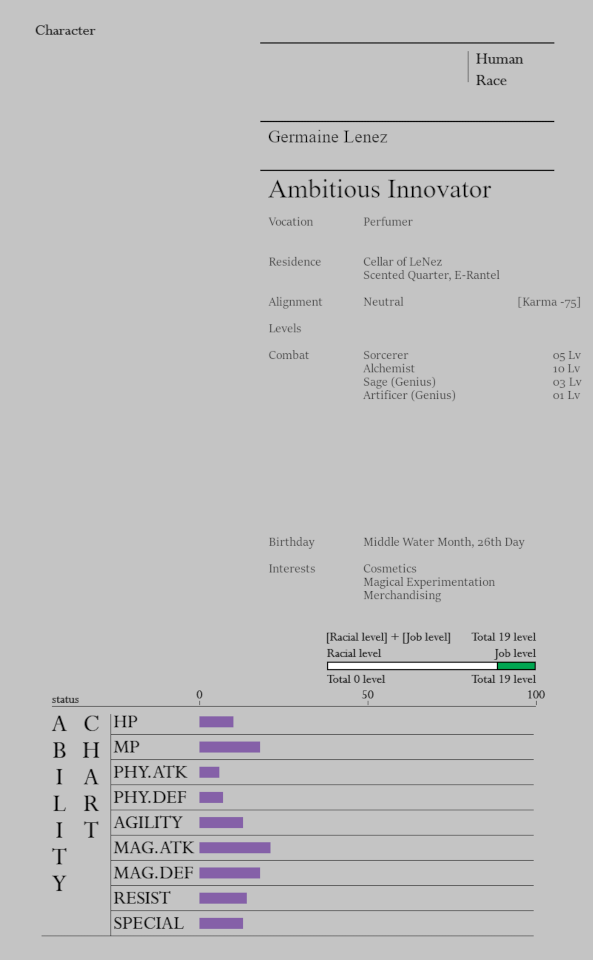
\includegraphics[width=1\linewidth]{V1 Birthright//images/ucThEId.png}
    \caption*{Germaine Lenez Character Sheet}
\end{figure}

\section*{Arcane Artisans}

Not all of those who are gifted with aptitude for the arcane become mages who seek their fortune as Adventurers, nor do they join the ranks of the armies or noble retinues of their nation. Neither do they become magisters that walk erudite halls to instruct on and delve into the great mysteries of the art.

 

Indeed, a great many mages do not even spare a thought to the vocations that may place them in mortal danger, or those of study for its own sake. They do not seek an Adventurer’s fame or the grand campaigns of mighty armies; nor the company of their fellows in seclusion from the unlearned and ignorant masses of the world.

 

Instead, they turn their considerable skills towards the production of goods and services for towns and cities, selling their wares to noble patrons and common labourers alike. No simple apothecary or dabbler in enchantment and artifice can match the expertise and quality of those who endeavour to become masters of their respective crafts.

 

From lifesaving potions and magical equipment to enchanted tools that improve the quality of daily life and labour, these artisans form one of the cornerstones of civilized societies around the world. Their endless quest for its improvement makes them integral to development beyond simple agrarian life, and their work often comes hand in hand with the rise of advanced and powerful nations.

 

Though their focus may lie in serving on the industrial side of civilian settings, they are still potent arcane casters that often wield the same spells as one would find used by an Adventurer or Military Mage, as their research leads them to seek out answers in every field of magic available to them. Many an ignorant belligerent or nosy official have found themselves burned, electrocuted, frozen or melted – even transmuted into useful materials by an incensed shopkeeper to exact payment for the disruption of their business.


\chapter{Ludmila Zahradnik}

Ludmila and Lady Shalltear rested on a bench placed in the shade of a tree that had been left to grow off the street near the Perfumer’s shop. The Vampire was idly staring at the clear afternoon sky while Ludmila was once again busy recalculating her once again obsolete budget.

 

“You seem to be taking this all in stride,” Lady Shalltear spoke as she watched the wisps of the remaining clouds drift away as they journeyed southwards.

 

“My head is still spinning from all this, actually,” Ludmila said. “Ninety-six platinum is a lot of money, is it not, my lady?”

 

“I wouldn’t know,” Lady Shalltear said. “I’m no more aware of the value of anything than I was an hour ago.”

 

“I’m sorry, my lady,” Ludmila apologized. “My mind is swamped just trying to keep up with everything. Ninety-six platinum is enough to feed, clothe and arm every villager in Warden’s Vale for an entire year. Or at least it would be, if they were still around.”

 

“Well, if you put it that way, it seems like it would be a significant sum for one of you…but you made it sound as if your territory is small; is this not the case?”

 

“It is,” Ludmila nodded. “There were only thirty households last summer.”

 

“And how does that compare to the other nobles?” Lady Shalltear asked.

 

“Corelyn Barony has around two thousand households, last I heard,” Ludmila dredged up the numbers from her memory. “Countess Jezne should have close to five thousand households in her personal demesne alone. Then there are five other baronies within her territory, but they aren't as productive as the Riverlands, so perhaps double that in the whole of Jezne County.”

 

She frowned and made a vexed noise.

 

“I guess once I actually look at the numbers from that perspective, it’s not so much. Ninety-six platinum would barely last two days if Countess Jezne suddenly had all of her production cease like it has right now. I suppose this is what most people see when they look at the nobility and their revenues: they think about what they would personally purchase for themselves if they had access to such wealth, with no obligations. Ninety-six platinum coins for an average city labourer is over twenty-five years of work.”

 

“Your demesne is vacant now,” Lady Shalltear said. “It seems like you do indeed have that much for yourself.”

 

“It belongs to House Zahradnik,” Ludmila stated. “The revenues of the demesne should go towards its development and growth for greater gains in the future. After hiring and providing for the manor household, purchasing the tools and other supplies for the labour force, and buying what is needed to maintain the village, I will still have the majority of this capital to work with. I need to see about attracting new tenants and investing in services and industries for the village to support the surrounding lands as they are developed.”

 

“You seem to have a clear picture concerning the future of your territory.”

 

“The frontier territories are far behind in development compared to the interior regions,” Ludmila said. “There is much to study and learn from what the other nobles have done. But what works for them may not necessarily work for me – I have a few ideas but, by and large, it will just be a lot of trial and error: which I suspect is where most of my capital will vanish.”

 

“For someone with such a progressive outlook,” Lady Shalltear said, “that sounded quite pessimistic.”

 

“I did not mean for it to sound that way, my lady, but after looking at the filled-out parts of the almanacs that the administration provided…if they are accurate, then the nobility cannot rely on their past to model the future.”

 

Seeing Lady Shalltear’s face turn blank in confusion, Ludmila realized how cryptic her last sentence sounded.

 

“It’s the Undead workforce, my lady,” she explained. “If the Sorcerous Kingdom can field this labour in quantities enough to fill the needs of every territory, then our economies are fundamentally changed. For a fraction of the cost of providing for tenant farmers, these Undead servitors can do the same work. The same goes for any other sort of menial labour that they can manage. That means we will need far fewer tenants working directly as labourers, and more tenants that are capable of directing the Undead in tasks that benefit from specialized direction.

 

The nature of value will shift drastically – any goods produced with the assistance of Undead labour will become cheaper relative to those produced by more complex tasks that still require the expertise of skilled craftsmen. Territories that have vast amounts of arable land will be able to thrive through sheer volume of agriculture, but those that do not will need to find or create something unique to their own territories that set them apart from the rest. Warden’s Vale falls into the latter category: for the time being I can rely on forestry and the limited agricultural space we have, but the terrain of the highlands makes development like you see in the interior difficult and expensive by comparison.”

 

Ludmila looked around at the empty street, continuing to share her thoughts with Lady Shalltear.

 

“The entire region will feel these changes, I think. E-Rantel is the hub of inland trade between Re-Estize, the Empire and the Theocracy. I’ve seen those that look like they come from places even further out as well. Once the duchy comes back to life and commerce resumes, the city will be swarmed with traders who will seize the opportunity to buy the goods that the Sorcerous Kingdom produces at significantly lower costs.”

 

“I think you’ve gotten so used to us that you forget that most people are rather averse to the Undead,” Lady Shalltear said.

 

“You are correct, my lady,” Ludmila conceded, “but, like this city, it should only be a matter of time. The most intrepid merchants will carry the Sorcerous Kingdom’s products far and wide, and their guildmates will see their caravans laden with commodities obtained at prices impossible elsewhere. Ambition will overcome fear – the only fear will be the fear of falling behind their rivals and competitors, and that will drive them all the more.”

 

“So...how long would you say until this happens?” Lady Shalltear leaned towards her, “This vision you conjure seems to fulfill a part of His Majesty’s wishes.”

 

“If trade is allowed to flow freely, a few years, perhaps,” Ludmila said. “Not more than a decade for the immediate region. The only obstacles that come to mind would be the political and cultural barriers that may form in opposition to the growing power of the nation – or the nature of the Sorcerous Kingdom itself. Since the Undead will be doing most of the menial labour, someone might spread rumors of cursed foodstuffs, for instance.”

 

“Those Skeletons are incapable of casting curses,” Lady Shalltear muttered. “We should find the individuals that spread these baseless rumors and silence them.”

 

“That is a needless effort which may cause more problems than it solves, my lady; it can be safely ignored, I think. Merchants will find ways around those barriers to facilitate trade, and even a formal trade embargo seems self-defeating. Over time, those that embrace our nation’s trade will thrive compared to those that do not due to the cost of our goods. If nations do not yield to this trade, they will slowly lose ground to their rivals until their lands are forcefully taken from them. So, sooner or later, they will fall under the Sorcerous Kingdom’s economic hegemony. If they wage war to break the hegemony, they will only provide the justification to be crushed by His Majesty’s armies.”

 

“Did you realize this all on your own, while sitting on this bench?” Lady Shalltear examined the rough wooden construction of their seat suspiciously.

 

“It is the knowledge and experiences of the past day coming together…and perhaps I have been raised in part to see things from this perspective for my entire childhood.” Ludmila’s gaze turned inwards. “Realizing possibilities makes you come into other possibilities. As resources become available and knowledge grows, things that I would not have not conceived of come into view. As each hour passes, my life seems to become busier – I want to see and do more, and the hours of the day seem ever more insufficient. Besides, that should be the reason why the annexation of this duchy came in the form that it did, yes?”

 

“Um...maybe?” Lady Shalltear’s gaze shifted away, “Some of the others should understand at least this much, but even the most intelligent amongst us can only hope to skim the surface of His Majesty’s limitless insight.”

 

“The laws of Re-Estize have been kept intact,” Ludmila stated, “which means that His Majesty has left the management of its territories to those that already have a firm grasp on the characteristics of their respective fiefs. The policies and mechanisms of the administration have been set up so that we can smoothly adopt the concepts that the Royal Court wishes to introduce to the nation so they can, in turn, realize their goals for industry and trade. As all of the pieces fall into place, this grand strategy will become an unstoppable current – one can either have it carry them comfortably to where it brings us, or be swept away forcefully to the same destination regardless.”

 

Lady Shalltear was silently mouthing something as she digested Ludmila’s words. Her expression suddenly sharpened, though, and she turned her head to the south.

 

“Oh, they found something,” she said.

 

“My lady?” Ludmila twisted around to look to the storefront to see if Aemilia had come out.

 

“Not them. The members of my Household that I sent to locate your ship.”

 

“Really, my lady?” Ludmila rose from her seat, “Where did they find it?”

 

“I don’t think I’ve seen a name for it on the maps. There’s a steep section of the valley, where the river goes through a series of large bends. The ship they see has run aground on the bank.”

 

“I know where that is…the shores are rocky though,” Ludmila frowned worriedly, “is there any damage, my lady?”

 

“They can’t tell,” Lady Shalltear replied. “Shall we go take a look?”

 

Ludmila thought for a moment before deciding to wait.

 

“We should wait and return to the house with the wagon, my lady.”

 

“What about the food you still have to sell?” Lady Shalltear asked, “The Merchant Guild as well, to collect your payments.”

 

“Seeing today’s revenues thus far, I can provision the city manor with it instead,” Ludmila answered. “It should be enough to keep the household staff fed for a while without needing to access the city’s limited supplies. We can drop by the Guild after we’ve seen to the vessel.”

 

As they made their way back to the wagon, the front door of the workshop opened. The heat and odours of its interior once again wafted out into the street and Aemilia emerged with a small, lacquered Rosewood chest held in both hands. One of the Vampire Brides was holding a smaller box with a similar appearance. Germaine followed after them, closing the door lightly behind her with a grin on her face.

 

“It looks like they found something for you as well, my lady.” Ludmila noted, but Lady Shalltear only tapped her lip thoughtfully.

 

The Perfumer came up to Ludmila and held up two sheets of high quality paper.

 

“This one’s the bill for what your Lady’s Maid purchased,” Germaine said as she handed over the first, then the second, “and this one’s the invoice for the Merchant Guild. You can move your wagon into the alley where we’ll grab the rest of your things and get those trees into the warehouse.”

 

Ludmila motioned to the Soul Eater to do as Germaine instructed, then looked down to the bill.

 

Aemilia had ordered quite a long list of items. There were two sets of women’s perfume for each member of the household staff – one set for use during functions held during the day, and another for those held during the evening. There were also a dozen vials of cologne for the manservants that would be hired; she wondered if the Undead footmen were expected to use it as well. She scanned over two crates of aromatic candles and one crate of scented soap as her eyes ran down the list to the end, where the items for her personal use were. Three sets of perfume, soaps, candles, bath salts and scents for her solar. She didn’t even know where to start on their use; her experience with fragrances was next to nonexistent, given the remote location of Warden’s Vale and the impracticality of using cosmetics that could easily make Demihumans aware of one’s presence.

 

Her eyes felt like they would roll out of their sockets when she read the tally at the bottom: eighty gold coins – eight platinum coins had disappeared before they had even entered her hands. She looked up with a question on her tongue, but Aemilia’s beaming face seemed so confident and pleased at her selection that Ludmila’s words were left unspoken.

 

“Is there one for me?” Lady Shalltear said as she peeked around Ludmila’s arm at the bill.

 

“Hmm…well that one’s a gift?” The Perfumer replied, “You said you were a Cleric, but if one of the city temples here had someone like you, they’d be overflowing with ‘supplicants’ every day. That means you must be a big shot on the King’s side, right? The Baroness here defers to you, after all. Just let people know what you’re wearing if they ask, and where it comes from. It’ll be great for marketing.”

 

“Lady Shalltear is the Minister of Transportation,” Ludmila informed her.

 

“Ahaha…”

 

Germaine abruptly turned around and quickly walked off after the wagon that had disappeared around the corner and into the alley.

 

Ludmila instructed the Death Knights to help with the cargo, then turned back to Lady Shalltear. She was holding up a clear crystal vial about the length of her pinky finger against the sky, peering at the liquid inside. She suddenly flicked the vial into the air, and it tumbled end over end before falling again to hit the stone pavement at her feet. Rather than shattering, it bounced several times before spinning to a halt. She knelt to pick up the vial again.

 

“The vial has a petty enchantment reinforcing it,” she noted with interest, “and since it has become a magic item, it won’t break without one purposely destroying it. How quaint.”

 

“What did they find for you, my lady?” Ludmila was curious about what the Vampire Brides found that they thought suited their mistress.

 

Lady Shalltear removed the stopper of the vial and turned it over against her wrist. After testing the scent with a focused expression, she extended her arm. Ludmila leaned forward: it was rich and earthy, with the hint of green and dried flowers. The ghost of incense could be detected, so faint that it gave the impression it was not actually there.

 

“A winter meadow? No, it wouldn’t have incense mixed in then,” Ludmila could not quite place the fragrance.

 

“A mausoleum,” Lady Shalltear offered, “or a tomb. The aroma of turned earth, dried flowers and incense in a long forgotten offering to the past.”

 

Her words came together with the fragrance of the perfume to create vivid imagery. Of cold stone in pristine silence; the peace of the grave seducing the weary to rest.

 

“It suits you very well, my lady,” Ludmila agreed with the selection. “Her quirks aside, Germaine is an excellent Perfumer…do you think she would accept an offer to move her workshop to Warden’s Vale? It is much cooler there throughout the year, and she expressed an interest in what could be gathered in the region.”

 

“If you believe so. I can hardly advise you in matters of your own demesne.” Lady Shalltear said, then smirked, “Though you may want to be able to survive an Acid Cone or two first.”

 

The rattling of the now mostly empty freight wagon drew their attention as the Soul Eater drove it back onto the street. Aemilia and the Vampire Brides were already sitting in their usual seat on the rear edge of the wagon. The Death Knights stomped out after them, but Germaine was nowhere to be seen.

 

“Where’s the Perfumer?” Ludmila asked them as she and Lady Shalltear pulled themselves into the front seat.

 

“Miss Lenez stayed behind in her workshop, my lady,” Aemilia answered. “She looked ready to get to work.”

 

“It seems like I will have to make my offer some time later,” Ludmila said, “not that I am in any way ready to accommodate an Alchemist. We are heading back to the manor to drop everything else off. There is something I need to check on before we go out to purchase the rest of what is needed.”
\chapter{Ludmila Zahradnik}

The sun was hanging over the battlements when the Soul Eater parked the wagon in the service lane behind the manor. After sending Aemilia into the house with their things, Ludmila instructed the Death Knights to carry the crates and barrels of food into the cellar.

 

“Is the ship still there, my lady?” Ludmila asked.

 

“This child came back right after they located it.”

 

Lady Shalltear pointed to the air above their heads, where Ludmila noticed a small black bat fluttering about.

 

“The rest stayed to guard the location,” Lady Shalltear told her, “so it should still be there unless it somehow dislodges itself and continues downstream.”

 

The footmen returned from their task and Ludmila directed the Soul Eater to meet her in the port village of Corelyn Barony. She fell in step with Lady Shalltear as they walked along, entering a service lane behind her manor.

 

“Are two Death Knights enough to move something that heavy?” Ludmila asked.

 

They left the service lane, and it turned out that the gardens between the clubhouse and the Royal Villa were not far at all if one cut through the back ways.

 

“Going by what was conveyed to me,” Lady Shalltear answered, “they should be able to work it off whatever it’s caught on. Are we ready to depart?”

 

“Yes, my lady,” Ludmila replied. “Thank you.”

 

“「Gate」.”

 

The familiar black portal opened in the air before them in the centre of the gazebo. At Lady Shalltear’s prompting, Ludmila stepped through. She blinked as her vision shifted from the surface of the gate to the filtered sunlight of the ravine that was their destination. It was close to where she had expected their location to be by the description that was given earlier. The river flowed down from the south, coming out of the steep gorge that started at the southern end of Warden’s Vale. Its flow was broad and deep, curving around the northern edge of the barrier ranges to meander its way eastwards towards the Katze Plains. She could see signs where people had waded to the shore, leaving prints on the riverbank and a trail of disturbed plants up and into the forest above.

 

The Death Knights appeared through the gate behind Ludmila and Lady Shalltear and her attendants appeared shortly after.

 

“Oh, it’s a Knarr,” Lady Shalltear said when she laid her eyes upon the vessel.

 

“Is that what this type of boat is called, my lady?” Ludmila asked, turning her attention back to the river. “We always just called it ‘the boat’ or ‘the ship’.”

 

“Even though you’ve used it for generations?”

 

“It is the only such vessel in use around here,” Ludmila shrugged. “I suppose there was no need to refer to it as anything else. How did you know what it was called?”

 

“One of the territories at home has several vessels of similar appearance,” Lady Shalltear said. “Still, it’s strange that you don’t even know what you’ve been using. How did it come into your House’s employ?”

 

“My ancestors found it mostly intact on this river somewhere. The villagers managed to refurbish it for transporting goods back and forth from E-Rantel…we never learned how to build more of them, but if what is claimed about the Undead labour in the administration’s materials is true, we will need more vessels like this to keep up with my fief’s production.”

 

Lady Shalltear’s gaze crossed over the boat, then looked out over the river.

 

“This type of ship is designed for travel on both rivers and large bodies of water,” she said. “Perhaps, if you travel further down the river, you will find out why it was here – perhaps you will find more ships to use as well.”

 

“It may be as you say, my lady,” Ludmila agreed. “Besides, one day I would like to see where the river leads.”

 

There was a mass of chittering in the air above, and she looked up to see Lady Shalltear’s Household fluttering down to disappear into the shadows surrounding her. The Vampire watched from an outcropping that overlooked the riverbend as Ludmila directed the Death Knights to extract the Knarr from its predicament. After it had been worked off of the hidden stones and placed fully onto the water, Ludmila stepped over the railing and into the boat as the Death Knights held it fast against the current. She walked up and down its length and hopped a few times in different places, but could not hear or feel anything amiss. Ludmila looked up to Lady Shalltear.

 

“I need to take the ship to the village port south of E-Rantel,” she called up to her, “would you like to join us, my lady?”

 

“You go on ahead,” the Vampire made a waving motion. “I need to prepare for the daily meeting of the Royal Council. I’ll find you after we’re done.”

 

“Ah…we may have to meet again tomorrow morning then,” Ludmila apologized, “the current in the spring is swift, but I will still only arrive some time in the middle of the night – or perhaps early in the morning.”

 

“That long? Can you operate this vessel between the three of you?”

 

“I don’t need the sails going downstream,” Ludmila said. “All I need to do is keep the ship away from the shore; the river is quite deep. Come to think of it, the navigators always preferred that I take the night watch...I guess I never realized why until now.”

 

Lady Shalltear looked down at them for a moment before floating down.

 

“Is something the matter, my lady?” Ludmila asked.

 

“Too long,” Lady Shalltear said. “You still need to buy what you need for your work in the barony, and we need to get your Undead labourers on their way.”

 

She looked over the Knarr, then out at the river again, at a point not far downstream.

 

“「Gate」.”

 

A black portal wide enough for the ship to easily pass through appeared in the river. The roar of churning water issued from behind it.

 

“This will take your ship to the section of river before the port,” Lady Shalltear told her. “I’ll meet with you after you return to the city.”

 

“Thank you, my lady.” Ludmila paused for a moment before asking, “What happens if I am unable to get the whole ship into the Gate?”

 

“I don’t think anyone has purposely tried that before,” Lady Shalltear answered. “I’d advise against you experimenting with it.”

 

Ludmila called the Death Knights to board the vessel and slowly steered it out from the shore as the current began to move them. Their course stayed true, until they started getting closer to the Gate. The water near the edges of their route was being drawn around the Gate due to the tumultuous current caused by the gap in the river behind the portal. She struggled with the tiller, trying to keep the vessel straight, but it started to veer and tumble on its axis. Fortunately, there was still enough space to fit through even while the ship was oriented at a strange angle.

 

On the other side, the abrupt change in current jarred the vessel after they left the Gate, throwing all of its occupants off-balance. One Death Knight was driven to its knees, while the other was thrown completely overboard with an unexpectedly quiet plop that was drowned out by the roar of the water leaving the portal behind them. Ludmila was painfully knocked into the tiller, causing the vessel to lurch violently even further and she leaned limply over it, winded by the impact. Through teary eyes, she recovered her footing and straightened the boat’s course once again as the portal silently shut far behind them.

 

Ludmila worriedly scanned the water’s surface, searching for the Death Knight that had fallen overboard, but there was no visible sign of its passing, nor anything at all to indicate where it actually was over the murmur of the river. Hoping it was still somewhere nearby and had not been carried far downstream by the current, she called out over the water, instructing it to follow them along the northern riverbank. A few seconds later, she sighed in relief as its horned helmet broke the surface of the water and it stomped its way onto the shore to follow them, armour glistening wetly in the late afternoon sun.

 

Leaning back tiredly into her seat, Ludmila placed a hand on her sore abdomen. Not far ahead, she saw the familiar sight of Corelyn Village’s earthen jetty. Like the one at Warden’s Vale, it had been built to deflect the river current and provide a calm harbour to moor vessels in. She directed the Death Knight on the shore to run ahead to the harbour and grab a large rope to throw to its fellow on the boat when they maneuvered in closer. Between the two sturdy Undead, the ship smoothly pivoted around the jetty, its momentum carrying it all the way into the calm waters of the port. As the boat lightly bumped up against the pier, she hopped off to secure it to its moorings.

 

While she worked, a scream drew Ludmila’s attention towards the village, where a girl had appeared from a building not too far from the shore. She turned in a panic, stumbling over her feet several times as she fled.

 

“Wait!” Ludmila called out after her.

 

The fleeing villager did not stop, even though Ludmila had unconsciously projected her ability along with the word. The girl did not even slow at her voice as she scurried away down the empty village lane, shedding doubt on her confidence that she could use her abilities properly. The sight of the Death Knights stomping after the girl to make her ‘wait’, however, did not give her much time to ponder. She hurriedly recalled them before inadvertently starting some sort of mass panic in Clara’s home village. The encounter had her decide against waiting on the Soul Eater at the port, and she led her footmen onto the highway to meet the wagon on the way.

 

She spotted the Soul Eater already galloping down the hill from the city. The roads allowed it to speed along without damaging the wagon and, within another fifteen minutes, it came close to where they awaited it on the highway. After it had turned the wagon back around towards E-Rantel, she hopped on and it took off back towards the city. Now that she was a passenger, the ride did not seem as smooth as it had looked when the wagon had come down the hill. As it was formerly a part of Rampossa III’s demesne, the highways had been paved, making them much better for carriages, carts and wagons to travel on. At the wagon’s current speed, however, Ludmila was vibrating so violently in her seat that she held worries as to whether the vehicle would shake itself apart before they returned to the city.

 

The Soul Eater assumed a canter after she became concerned enough to tell it to slow down and, a little over thirty minutes later, they arrived at the massive main gate of the city. The two Death Knights on either side of the entrance looked towards her briefly before returning to their watchful vigil. They did not move to impede her as she entered, and the wagon thankfully rumbled through at a much more reasonable speed than it had taken north along the highway.

 

As they crossed into the military district that lay between the outer and second walls, it occurred to Ludmila that she had forgotten all about her labour force. Standing up as the wagon rolled by where they were ordered to wait, she spotted them neatly arranged exactly where they should have been. She sat back down, feeling a bit guilty about neglecting them for so long, but at the same time wondering if they would wait forever if they were just left there.

 

The wagon made its winding way through the thoroughfares of the city towards the main plaza, and Ludmila looked up towards a familiar, barely audible chittering noise – a small black bat fluttered above them. Further above, she spotted the Elder Lich, who might have been trailing her the entire time. She wondered if the Imp was lurking about somewhere as well. She was about to order the Soul Eater to stop and see if Lady Shalltear would appear when her liege suddenly alighted on the front of the wagon, the lacy frills of her gown fluttering in the wind. Without a word, she once again seated herself beside Ludmila, as if dropping out of the sky in such a manner was perfectly normal.
\chapter{Ludmila Zahradnik}

Ludmila stared over at Lady Shalltear, whose crimson eyes had taken on a dim glow in the fading light. None of the Undead around her reacted or even seemed to care that someone had fallen out of the sky, and Ludmila started feeling a bit out of place being the odd one out.

 

“My lady,” Ludmila asked, “will it become a normal thing in the city to have people landing in the street like that?”

 

“There are many Heteromorphs and Demihumans who have the ability to fly,” Lady Shalltear said. “Magic users and wielders of magic items enchanted with flight spells also do so…so it should be a more common sight in the future as more peoples fall under the dominion of His Majesty.”

 

“There are no laws regulating flight in Re-Estize,” Ludmila said. “Perhaps you should propose a few as the Minister of Transportation to prevent incidents in the future. I cannot imagine airborne accidents ending very well for anyone involved – or the people below.”

 

“The sky is quite vast,” Lady Shalltear replied, “and the chance of randomly bumping into others is much lower than walking on a street…but I suppose something should be in place to prevent potential damage to His Majesty’s realm.”

 

“You have never collided with someone in flight before?”

 

“Only when I’m aiming for them,” Lady Shalltear smiled.

 

Ludmila shook her head, uncomprehending. Meanwhile, the Soul Eater turned as it entered the still-empty main plaza, driving the wagon towards the front of the main office of the Merchant Guild. It was a grand structure of three stories, occupying the entire side of the plaza where it had been constructed. Windows of clear crystal lined the second and third levels of the building, which would offer a glimpse of the archives and offices within. The main entrance had two pairs of glass doors at the top of the broad granite stairs leading up from street level.

 

The imposing building stood directly across the plaza from the city’s main cathedral, which had been sponsored by the Theocracy at the site of the original chapel that had been built when the city was founded and Re-Estize was still young. The guild office was not only placed across from the cathedral, it was also built at the same height as well – as if daring to challenge the might and authority of the Temples. The fountain and column that they had passed between on the way to the outer reaches of the district were a reminder that this rivalry was very much real. When the main office of the Merchant Guild was constructed, it was said that the Temples commissioned the beautiful fountain on their side of the plaza to remind the citizens of the life and provision that the gods provided. But then the Merchant Guild had raised the column: an elegant work of art which dominated the square.

 

Years ago, she had overheard a conversation amongst the ladies of the nobility concerning the rivalry between the Merchant Guild and the Temples. That E-Rantel was a city of trade and in the secular government of Re-Estize, the power of the Temples was dwarfed by the influence of the Guild. Because of this, the Temples were said to be perpetually jealous, but could only make ineffectual motions outside of their direct spheres of authority. Worship of the Six Great Gods had long since waned in the north with the rise of the faith of The Four, but the situation remained the same: commerce was the lifeblood of the city, and the Guild was its beating heart.

 

That heart seemed still now. The gleaming head of the column caught the light of the evening sun over the rooftops, scattering its shimmering radiance in bright fragments over the plaza, but the Guild Office itself appeared as silent and inactive as when they had crossed the main plaza earlier that day. The windows that peeked into the archives and offices had their curtains drawn shut with no light visible behind them. There were no clients entering or leaving the building, nor anyone resting on the stairs or benches outside.

 

As Ludmila stepped off of the wagon and approached the main entrance, she saw that there was a single light visible from the entrance, where a balding man stood at one of the reception counters. The large door was light and soundless as she pulled it open for Lady Shalltear, and the measure of their footfalls whispered on the long carpet as they approached the front desk. The old man made no move to recognize them – his head was bent over the unadorned counter as he leafed through the thick binder that lay in front of him. It was only when they had come directly in front of his stall that he raised his head. Sharp brown eyes that belied their owner’s apparent age looked over to Ludmila; then to Lady Shalltear. His gaze then went down to their hands before finally settling on the blue folder in Ludmila’s possession.

 

The old man looked Ludmila in the eye and spoke in a clipped, yet decisive tone.

 

“What business do you have with the Guild?”

 

Unsure on how to respond, Ludmila opened her folder, retrieved the two invoices within and placed them on the counter. The man immediately took the sheets of paper, holding them up in his lean hands towards the light. It took him a minute to scan over the first invoice, after which he switched to the other. He then walked over to a long table behind the counter, flipping through another binder which lay there. After a few more minutes, the man returned to the reception counter. He rolled a large stamp over an inkpad, and pressed it onto both of the invoices. Ludmila thought she saw the ink glow briefly before he placed his palm over the invoices and spoke.

 

“Do you have an account with the Guild, Baroness Zahradnik?” He asked.

 

“I am not a merchant,” she replied.

 

“You don’t have to be,” he patted the invoices. “Anyone that does business like this should register with the Guild.”

 

“Why is that?” Ludmila asked.

 

“Have you ever seen someone pull a hundred platinum coins out of their pocket?” He tapped his finger on the Perfumer’s invoice.

 

“Well...no,” she admitted.

 

“Me neither,” he said. “That’s what the guild does. You don’t carry coin around doing business like this: you just use invoices like the ones on the counter here. The Guild ensures that each transaction is authentic and then the money is transferred between accounts. The only time people move real coin around is with an armed escort to places where there’s a need for it.”

 

“What about all of the people in the city that trade in coin?”

 

“We usually don’t deal with them,” he said, “but we do deal with the merchants that take their coin and deposit it here. The Guild mostly deals with real money, sums of Platinum like these invoices or even greater.”

 

“It goes higher than Platinum?”

 

“Sure does. Mithril and Adamantite coins. Gem coins and official plaques of credit. You don’t see that around here though. Too poor.”

 

Just this morning, Ludmila was agonizing over how to budget out a few hundred gold coins to supply her demesne. Now, after she had come into wealth she had never seen before, much less expected to possess so soon, this man was telling her that platinum was the smallest denomination of currency that they normally dealt with, and that the largest trade hub in the nearby region was considered too poor to deal in anything greater.

 

“Alright then,” she said, “how do I register an account?”

 

“You’ll need to provide proof of your identity and a seal so we can add it to our archives for authentication purposes,” he replied.

 

“But you just addressed me as Baroness Zahradnik?”

 

“A courtesy.”

 

“Then what do you deem suitable as proof of identity?” Ludmila asked.

 

“Official documents from the administrative office that you report to,” he said. “Or you can have an official vouch for your identity.”

 

“Oh! I can do that,” Lady Shalltear said from beside her.

 

The old clerk turned his attention to Lady Shalltear, whose shoulders barely appeared above the counter.

 

“...and you are?”

 

“This is Lady Shalltear Bloodfallen–”

 

“Never heard of her.”

 

“Lady Shalltear is the Minister of Transportation.”

 

“Lady Shalltear will need to provide proof of her identity and provide a seal so we can add it to our archives for authentication.”

 

“Lady Shalltear is about to turn this entire building into a heap of cinders with a Fire Storm spell.”

 

Seeing her liege’s mood take a turn for the worse, Ludmila hurriedly attempted to deescalate the situation.

 

“A moment please, my lady,” she implored Lady Shalltear in placating tones.

 

She turned towards the entrance and paced hurriedly towards the door. When she stood at the top of the stairs outside, she looked around for the Elder Lich. Spotting it floating above the plaza, she waved for it to come down.

 

“Do you have proof of identification and a seal of office as a member of the administration?” She asked.

 

“Yes,” it said.

 

“I require your assistance, then. Come with me.”

 

Ludmila turned back to enter the office, hoping that she was fast enough to prevent whatever a Fire Storm spell was from befalling the building. Fortunately, Lady Shalltear did not appear to be casting anything when she returned to the counter – but, upon seeing the Elder Lich with what was needed in hand, her expression darkened even further.

 

“The official here can vouch for our identity,” she motioned for the Elder Lich to come forward, “are these credentials acceptable?”

 

The attaché placed what appeared to be a small plaque and an ebony seal on the counter. The old man raised the items to the light no differently than he had the invoices, and there was no sign he even cared that an Elder Lich had walked up to him. Shortly after, he placed them back on the counter and produced two identical forms from somewhere out of sight below the desk. Ludmila filled her form and stamped it with the seal that she had brought with her from Warden’s Vale. The seals of the Merchant Guild and the Civil Office of the Sorcerous Kingdom followed soon after.

 

They moved to work on Lady Shalltear’s documentation, but when the Elder Lich raised its hand to stamp the form, the Vampire shouted.

 

“Wait!”

 

Three heads turned to Lady Shalltear at the interruption.

 

“Not you.” she said to the Elder Lich, “You.”

 

Ludmila found Lady Shalltear’s finger pointed towards her.

 

“My lady?”

 

“You can vouch for me and use your seal on the form,” Lady Shalltear said. “You had your identity verified by this attaché, yes?”

 

It seemed needlessly convoluted, but Ludmila acquiesced. The guild clerk disappeared into the office, shaking his head, after which Lady Shalltear spoke.

 

“That gorilla did it on purpose,” she said testily.

 

“What is a ‘gorilla’, my lady?” Ludmila asked.

 

“It’s – never mind. The Guardian Overseer is making things hard for me on purpose. There’s no way she didn’t know that I would need these things eventually, and then she sent this Elder Lich with everything that you need as your ‘attaché’ to serve as a constant reminder of her influence even as you are subordinate to me.”

 

“Lady Shalltear,” Ludmila licked her lips as she tried phrasing her question tactfully, “are there…issues in the Royal Court?”

 

“Issues?”

 

“You seem to have a rather disagreeable relationship with the Guardian Overseer.”

 

“Ah, that’s what you mean,” Lady Shalltear said. “We are rivals, not enemies. There is solidarity when it comes to the Will of His Majesty and the defence of His realm.”

 

“Then...if I may ask, my lady,” Ludmila was still unsure if it was a delicate subject or not, “what is the nature of this rivalry?”

 

“The only thing that matters, of course!” Lady Shalltear said matter-of-factly, “To earn our place at the side of His Majesty, in all things. Do ambitious Human nobles not seek great achievements within their courts? To win the appreciation and trust of their liege?”

 

“In many things, yes, that is the case, my lady,” Ludmila replied.

 

“This rivalry can become a bit…intense sometimes,” Lady Shalltear said, “but it has never grown to the point where His Majesty’s realm has suffered for it.”

 

“Thank you for the explanation, my lady. I will keep this in mind.”

 

As they waited in silence, Ludmila looked at the Elder Lich that had stood on the other side of her for the entire conversation. It displayed no reaction to the accusation that it had been dispatched as a form of harassment. She heard shuffling steps as the old man reappeared. Ludmila turned to face him as he placed several documents between on the polished counter, pushing them forward.

 

“These are the relevant templates that you should use when drawing up bills and invoices related to Guild business. Make sure that the staff that you assign to work with us are familiar with the format.” He straightened after his explanation, “Your registrations with the Guild are now complete and your account balances have been updated. These are your balance books. Is there anything else you need, Minister Bloodfallen? Baroness Zahradnik?”

 

Ludmila reached out to take the small booklet bound in black vellum. She opened the unmarked cover: the front page was similarly blank, but the next page had rows and columns lined upon it. Written on the first row was the balance of her account with the Merchant Guild. Between the invoices from Gareth Boyce’s lumber yard and the LeNez workshop, House Zahradnik had received 108 Platinum coins. It was an amount she had never thought she would ever have available to use at once. The digits were written in simple cursive, but they represented a responsibility that she would now need to wield for the prosperity of her demesne.

 

“I need to purchase tools for farming and forestry,” Ludmila asked the clerk waiting patiently across the counter. “Is there an open business where I can find those?”

 

“Just head to where all the forges are,” he told her. “If there are any working, you’ll definitely notice.”

 

The answer seemed obvious, after the fact.

 

“When is it appropriate to deposit and withdraw at the Guild?”

 

“There are no set rules on that,” he replied, “but as a general guideline, any amount that you feel unsafe carrying around.”

 

“Can the guild be used to hold coin for anything?” Ludmila asked.

 

“Yes,” the clerk nodded. “We prefer it that way, in fact. It’s easier to deal on paper, but a lot of people can’t trust that. Unless you’re a high noble, you probably can’t afford the type of security that the guild has. The new King has also contributed some of his soldiers to ensure that the wealth of the city remains secure.”

 

“Then you don’t mind if wages and such are withdrawn by my staff?”

 

“Mmh,” the clerk grunted. “Petty amounts should be withdrawn as part of a lump sum. We’ve a few members that send escorts with their agents to collect wages for the whole of their staff to be distributed at their business or homes. You should do the same.”

 

“Is there anything I should avoid doing?”

 

“Nothing illegal: you’ll be reported to the relevant authorities if you do,” the clerk said. “If there are any other transactions that run afoul of guild regulations or seem suspicious, you’ll be informed as well.”

 

It nearly felt to her a barb, though the man probably did not know. If House Zahradnik had used the services of the Guild instead of relying on themselves, generations of financial hardship might have been circumvented altogether. It brought to mind something that she had thought about shortly after learning the depressing reality.

 

“Does the Guild recommend merchants?” She asked, “I would like to hire staff that can manage the commercial transactions for my demesne.”

 

“Hmm…we set up apprentices with masters, but it’s rare that a noble comes looking. They usually employ the ones from their own fiefs,” the man scratched his chin as he thought. “The city’s had a pretty good shakeup, so there might be some loose ones available.”

 

He fished up a blank sheet of paper, placing it on the counter between them.

 

“Put down what you’re looking for here. The types of goods and services you’ll be dealing in, compensation, licenses you’re offering, security arrangements and such.”

 

Ludmila’s borrowed pen scratched over the paper for several minutes as she tried to think of everything she might need. When the old man read over her requirements, his eyebrows rose.

 

“I’ve…never seen a request like this before,” he told her. “Nobles usually hire their own merchants to assist with managing things, but you’re looking to put one on retainer to help handle the business of your fief. Most nobles are passable at dealing with their own territories, so they tend to have a hand directing their own production and trade. If it comes down to it, they’ll have one of their children trained as a professional merchant to run the family business.”

 

“House Zahradnik has never been known for being merchants,” despite herself, Ludmila still nursed some of the bitterness from the afternoon in her heart. “I will have my hands full directing the development of my fief, so I would feel much more comfortable if there was someone to take care of this end of things…several such retainers, if necessary.”

 

“Well, any merchant will hire apprentices and assistants when business is good, so it should be the same for whoever you take in, except that apprentice will become a member of your retinue as well. Most merchants can’t do better than what a noble’s retainer gains through their service, but the sudden exposure to authority and wealth is sure to get into most people’s heads. I’ll see what I can do, but I wouldn’t hope for anything spectacular – especially with things as they are right now.”

 

Ludmila nodded at the response. The old clerk’s reply brought her to her last question.

 

“I understand,” she said. “Send word to my residence in the central district if you find anyone appropriate. There is just one last thing both the Minister and I would like to know.”



“And what is that?”
 

“The city has become…paralyzed after the duchy changed hands,” Ludmila said. “The markets and shops are closed and, barring the few places I’ve found, the various industries have become silent as well. How is it that the Merchant Guild remains open? Or more to the point – how can you still stand and serve clients here, when nearly all of your associates still hide in their homes?”

 

“That’s simple,” the clerk didn’t even bother to stop and think before answering, “the city is open, so the Guild is open. In our line of work, we deal with the fear that comes with opportunity and risk every single day – those that lose themselves to their fear have no right being here.”
\chapter{Ludmila Zahradnik}

The cool air of the spring evening greeted them as they left the Merchant Guild and descended the stairs to where the wagon awaited in the plaza below. Ludmila flipped through the materials that she had received from the clerk briefly before returning to study the invoice template. The paper was more sturdy and thicker than a normal sheet would be, feeling slightly heavier in her hand; it was designed to be durable as a long term reference to create duplicates from. She had a thought and turned to the Elder Lich.

 

“Are you able to create copies of this template?” Ludmila asked.

 

She held out the sheet, and the Elder Lich immediately took it into its hand.

 

“Easily.”

 

The Undead attaché’s raspy voice held no apparent emotion as it spoke, but the near instant reply gave the impression that it had scoffed at her question.

 

“I need five copies for this evening,” she instructed her attaché, “and fifty additional forms by the morning.”

 

It faced forward and set about its task as the wagon rolled off towards its destination. The flutter of leathery wings turned Ludmila’s head towards the Elder Lich again as the Imp alighted on its shoulder. She watched as her attaché held out a solid board that it had produced from somewhere to use as a writing surface. The Imp deftly drafted the first copy not long after as the pair floated forward alongside the wagon. They studied the work together and, after finding the results satisfactory, continued their task.

 

“Is it really necessary to have that many copies at once?” Lady Shalltear voiced her question as the shadows of the eastern quarter fell over them.

 

“They are for the residence in the city, my lady,” Ludmila replied, “if my household needs to order anything or do any other business on my behalf, they will be able to use the account at the Merchant Guild if I prepare forms in advance. The manner of conducting transactions that the clerk described seems to have fewer faults than simply handing over a bag of coin to be kept in the manor.”

 

“You don’t trust your servants?”

 

“Well, I have barely known them for a day,” Ludmila said, “though even if they had earned decades of trust, the system in use by the Guild still seems far more elegant overall in function. Out in the barony, there will be a need for funds on hand so it will be the usual methods there.”

 

“The lives of Humans seem filled with uncertainties,” Lady Shalltear shook her head. “You cannot trust your servants and your purpose in life is undefined and seemingly ever changing.”

 

“You are able to always fully trust your servants, my lady?”

 

“Of course. All the way down to the lowest being. They are bound to me – inextricably a part of my realm. Having them turn on me of their own will would be as inconceivable as your legs walking off without the rest of your body of their own volition. Deception in crucial matters is unthinkable, as is failure,” Lady Shalltear’s gaze observed the surroundings that they travelled through. “Yet Humans can ignore their obligations so easily. So few continue to function in this city, while the rest neglect their roles in your society to the eventual ruin of all. I’ve even witnessed those that would turn on their fellows, if only for a moment’s reprieve from their hardships.”

 

Ludmila listened quietly as her liege spoke. That everyone who served her could be treated with such confidence felt fantastically unrealistic. It was no small wonder that the Royal Council would be frustrated with the seemingly unreliable citizens of the duchy if this was truly the case. Perhaps the Sorcerous Kingdom would always look down on their Human citizens, as the current issues were the result of Human nature rather than any willful resistance or insubordination.

 

“It is difficult to refute your words with things as they are, my lady,” Ludmila said, “though I had not realized there was such a difference between the Human realms and your own. His Majesty shows great insight to have retained the laws of the realm, even when considering his existing vassals. Rather than have them directly dealing with the unfamiliar in an effort to manage the population directly, his decision allows those accustomed to the workings of their own to make changes smoothly.”

 

“Then what am I to do with you, I wonder?” Lady Shalltear turned her face towards Ludmila, eyes glowing at her as they went from shadow to shadow, “you are now mine – an odd vassal that does not quite fit in with the rest.”

 

Uncertain of where she now fit into the grand scheme of things, Ludmila could not answer.

 

“In many ways,” Lady Shalltear continued, “you are much like me in your role as a frontier noble. You guard the realms of your liege in a roughly similar function as my own in defending His Majesty’s realm. It can even be said that your burdens are far greater. You have not been gifted with great strength, nor vast intellect or powerful magic. Your demesne does not possess strong fortifications or armies. You are ignorant of the world beyond your borders and you are pitifully weak, but you will toil and struggle and fight and die against any and all intruders that would come, as your House has done for generations. Yet, for all of these efforts, your names become as dust to those that reap the benefits of the peace that you win for their lands.

 

In many other ways, you are different. You have ambitions beyond the immediate service to your liege, and you act as if it’s a natural thing. You actively seek the strength of others with the understanding that you’ll never truly be able to fully trust them. You are ultimately Human, and bound to your Human nature.”

 

Ludmila was at a loss as her liege conveyed the evaluation. She thought Lady Shalltear had followed her mostly to learn about the city and its workings as well as possible solutions to the predicament that it faced. Ludmila had not realized that she herself was being carefully watched the entire time as well. For all of her strength and influence, the Vampire had kept mostly to herself throughout the day as she had quietly observed her. She thought of the tales of another Vampire, Landfall, and wondered if Lady Shalltear’s behaviour was due to being a wise and perceptive Cleric, a predator accustomed to stalking their prey, or perhaps both.

 

Ludmila pondered her liege’s words, trying to find an answer they could both find satisfactory.

 

“My lady, the relationship between a vassal and their liege is maintained by contract.” She began tentatively, “For most nobles, especially those of the interior, it has become a sort of formal negotiation where those long established in their rule find agreeable terms between themselves. This contract – a pact of oath and obligation; duty and fealty – is the foundation of noble society and these realms by extension. It is the core of the relationship between liege and vassal, be they king and noble vassal, or landlord and tenant.”

 

“Go on…” Lady Shalltear had her chin in hand, looking up at Ludmila as she spoke.

 

“Nearly two centuries ago,” Ludmila continued, “when people came to settle the lands that would become Re-Estize and Baharuth today, there were no ties of blood, culture or trade that bound society together. There were only the leaders who established themselves over their people, carving out borders and defending their lands against any and all that would challenge the order that they sought to establish in the wake of the Demon Gods. These were the founders of the aristocracy of the Human nations of the north – nobles not unlike the frontier nobles: great captains of men and militant in both mind and disposition. The most prominent houses became the Marcher Lords: many of which you still see holding these titles today, though they mostly no longer carry the same traditions as their ancestors.

 

One house – the House of Vaiself – eventually unified the lands through diplomacy or war and the nobles who fell in line formed contracts between themselves and the throne. These contracts defined the relationships between House Vaiself and their vassals, continuing down the hierarchy of administration to form the foundation of Re-Estize. This contract, the oath of fealty between liege and vassal, is the core of what it means to be a noble of these lands: without it we are not much more than simple despots.”

 

“So what do these contracts look like?” Lady Shalltear asked.

 

“Well…I had thought to bring ours with us but decided to leave it at home since the duchy was fully ceded to an entirely new sovereign. That contract is effectively void now, but some may attempt to have old contracts ratified under their new liege in order to retain certain privileges from the previous government. I suppose since the transfer was so…clean, it would encourage at least a few to try.”

 

“Ah, so that’s what that was all about,” her liege seemed to remember something.

 

“My lady?”

 

“That noisy Count,” Lady Shalltear had a decidedly unimpressed look as she recalled the memory. “Fassett or something. Once it was clear that E-Rantel would see a bloodless transition, he came into the council chamber – bold as you please – demanding that his rights be recognized. As you might imagine, he got a rather cold reception: Cocytus flung him into the Gate that I opened even as he continued shouting about it. Considering how hard he was thrown, he probably didn’t survive the landing.”

 

“I thought there was only one place where you could use teleportation spells in the central district.”

 

“He came quite quickly. We were still implementing the framework for the government and finalizing security arrangements.”

 

“The Royal Court did not even wait to hear him out, my lady?”

 

“Oh, we did,” Lady Shalltear said. “He was very spirited, so we thought that this noble who had approached us before we even officially started our work must have possessed some merits. It was mostly preposterous, though – I think the disappointment added to his velocity.”

 

“Then what did he say?” Ludmila asked.

 

“Hmm…a few things that should have been a given: faithful service, some amount of taxes, the pledge to provide a levy, tributes for special occasions.”

 

“These are fairly standard in an oath of fealty,” worries began to mount in Ludmila’s mind, “though the details may vary…what did the Royal Council find offensive, exactly?”

 

“Well, he did deliver it in a very loud and presumptuous manner, but there was also his list of demands. In addition to the guarantee of his title, he wanted ownership of the abandoned territories bordering his own. Then there was the obligation to have His Majesty stand in his defence in court, as well as the full protection of all of his armies, the rights to enforce regulations upon the Guilds and control over the western highway that ran through his fief. He went on for quite some time, but I lost interest partway – the man was clearly not going to survive his audience.”

 

It was a mix of demands that were mostly within the realm of reason, though the expansion of territory and control over the Guilds was brazenly overreaching at best.

 

“Lady Corelyn mentioned something about other nobles vanishing as well,” Ludmila said. “Did they end up like Count Fassett?”

 

“Not that I can remember,” Lady Shalltear said. “Some fled their holdings after their audience – we didn’t care to detain them since there was no point in keeping administrators who were willing to abandon their responsibilities. The remaining nobles were advised to avoid committing the same offence as Count Fassett.”

 

“So none have attempted to reinstate old contracts or create new ones?” Ludmila frowned.

 

“Not a one,” Lady Shalltear replied. “Though I don’t even see a point to your asking. Some of what Count Fassett either offered was what should already have been a given and he asked for the same. Everything else was anywhere from incomprehensibly greedy to outright blasphemous.”

 

“It is still an integral part of a noble’s life,” Ludmila said. “Without it, the relationship between vassal and liege remains undefined and we are effectively without purpose. Some nobles need to add uncommon clauses to their contracts as well. Frontier Nobles, for instance, pledge to protect the realm’s borders. Since their territories are usually not that well developed, their liege is expected to put together a stipend from the other nobles in the demesne that benefit from their protection in order to maintain security. Is that so unreasonable?”

 

“No, not at all,” Lady Shalltear replied. “But it is not rooted in selfish greed like the terms Count Fassett dared to push on His Majesty.”

 

“So you would say that arrangements which are reasonable for the fief in question, or benefit the realm as a whole are acceptable?”

 

“Of course, but you had better be prepared to provide an explanation if I ask.”

 

“I think we should sit down together at some point and work this out, my lady,” Ludmila was still uncertain of what was safe to ask. “I do not want to inadvertently add some clause that would result in being thrown to my death if I can avoid it. It can come after I have done all this though – I still do not know what His Majesty wants from the nobility for the long term.”

 

The Soul Eater brought their wagon around a corner, where a large workshop of brick and stone occupied most of the city block. During their conversation, they could hear the sounds of the forge working out of sight as they approached from down the street, so the conversation invariably wound down.

 

“You’re probably thinking too much,” Lady Shalltear said. “You Humans are weak, and military support in the fashion of your former arrangement means little to nothing. There are those that would say that being productive and paying your due is good enough.”

 

Ludmila’s heart sank at the words, and she shifted uneasily in her seat. Her original expectation when Momon had delivered the royal missive in Warden’s Vale was that she would continue to carry on in the duties of House Zahradnik, much like how her family had served House Vaiself. However, nothing she could offer seemed to mean anything – indeed, the Royal Court’s perception of what held value was foreign to her own. A gaping void in her identity had suddenly appeared, and there seemed to be nothing that she could fill it with.

 

Lady Shalltear had described herself serving a similar role in the Sorcerous Kingdom to her own, so Ludmila was hoping that she would be able to empathize with her situation somewhat.

 

“And you, my lady?” She asked, her hopes dimming, “What do you think of this?”

 

“In all honesty, I don’t really see any point to it,” her liege answered, “but it is His Majesty’s Will to give Humans their…space. His ways have ever always eluded us in their entirety, so perhaps there are some things that we may not understand or appreciate yet.”
\chapter{Ludmila Zahradnik}

Ysbrant Mesmit grumbled to himself as he walked up and down rows of pallets piled high with spears, tightening the ropes that secured the oiled tarps laid over them. The hardened earth in the shadows of the makeshift lanes were still damp with the rain from the previous evening, and he could see laden clouds once again rolling down over the distant foothills of the Azerlisia Mountains to the north. He thought he heard the rumble of thunder carried on the evening winds and picked up the pace of his work – the last thing the shop needed was to have one of the protective covers ripped away by the stormwinds and his inventories exposed to the deluge that was sure to come.

 

After he was satisfied that everything was tied down properly for the night, he made his way back to the forge complex, stomping his heavy boots as he crossed the open yard in an attempt to dislodge the mud. He reached the first door and stopped, grunting in annoyance – the habits of his usual routine had brought him to the mill first, but the building had already been locked up for days. Events since the autumn had thrown his entire business into disarray as the patterns of industry were cast to the winds.

 

The space that was filled with spears was supposed to be the ore yard for the mill, but they had long since run out of ore to process. The spears in the yard were originally an order for the Royal Army, but the army had been routed on the first day of the annual skirmish with the Empire and so the majority of the weapons were left unclaimed and unpaid for. The confrontation itself had been pushed back from autumn to late midwinter, upending the usual cycle of production for the city’s forges.

 

They had to switch their efforts from forging spears to rushing tools and parts for all of the duchy’s territories that had suddenly found themselves with unexpected, additional manpower to perform their regular seasonal work. Then the advance orders from the Royal Army came in, forcing them to suspend the work they had switched to in order to fill the mounting demands of the nobles that were coming with their levy of hundreds of thousands of men.

 

His grumbling turned dark as he thought of all the wasted fuel and labour. The spears were now slowly being turned into plowshares, shovels and other tools as he could do nothing but redirect his workers once again to prepare for the planting season. Sheltered in buildings out of sight and away from the streets occupied by the Undead, they worked long hours into the night in the effort to reverse their bad fortune.

 

The faint sound of an approaching wagon turned his attention away from his grousing. He left the door to the mill and jogged across the yard to the main gate, unlatching it and pushing it open slightly before heading to the warehouse nearby. He grabbed a clipboard that was hanging just inside the entrance of the building and turned around just as the sound of the approaching vehicle stopped in the alley on the other side of the wall. A shadow separated from the one cast by the wagon, which was shortly joined by a second. Ysbrant straightened his posture as light steps approached the gate.

 

Rather than a merchant and his assistant or a pair of noble retainers, however, two finely-dressed women slipped in through the opening provided. The first was a moderately tall and slender young woman in her teens. Her forest green dress with few flourishes gave the impression that she was attempting to balance a feminine appearance with an outfit functional for more mundane activities.

 

The second woman projected an image which eclipsed the first’s. Though she only stood below her companion’s shoulder, she had a stunning appearance that would have drawn longing gazes everywhere she went. Her own outfit seemed incalculably valuable: an elaborate ballroom gown seemingly woven from silken shadows that devoured the evening light.

 

Their attire was in stark contrast to the rough and dirty surroundings of the forge. He had not seen the second woman before – with her unforgettable appearance, he would have had to have gone senile to not remember her – but the first seemed familiar somehow. After considering that she was just barely an adult, he was finally able to put a name to her face. She was taller since the last time he had seen her.

 

“Hm...the Zahradnik girl, isn’t it?” His voice came out gruffly, “In that fancy dress that your brothers complained about too. Here to use your allowance to buy a spear this time?”

 

Surprise briefly passed over her face at his recognition before she smiled slightly and spoke.

 

“My brothers must have said something memorable for you to remember that.”

 

Ysbrant grunted and he scratched the stubble on his cheek. The girl had a disposition much like her father’s – casually receiving his jabs and returning with an unruffled reply. Her companion showed no reaction either way, scanning the contents of the yard as if a workshop lot was an uncommon thing.

 

“So, what are you here for?” He asked.

 

“I need to purchase tools and parts,” she replied. “Do you have any in stock?”

 

Upon hearing her request, he sucked in his lips and stood in silence for a while. That she had come personally without any of her family seemed like bad news. Considering the fate of most of the Royal Army that winter…well, it was probably better left unspoken – he was already worried that he had unwittingly slighted her by reopening recent wounds, unaware of her family’s fate.

 

“I see.” He finally replied as he turned around to pull open the warehouse doors, “Well, take your pick.”

 

The space inside was filled with equipment, tools and parts for all sorts of labour. The women looked about silently as he continued speaking.

 

“It’s already spring, but no one’s come to buy anything,” he explained as he led them through the building. “Plenty of nobles should’ve sent in their orders by now and we’d be pushing our goods out nonstop, but production’s about to stall for lack of proper storage since no one actually is.”

 

“It looks like your workshop is still running, though.” Lady Zahradnik said as she handed her order to him and turned to motion for someone in the direction of the gate to bring in her wagon.

 

“A forge is expensive to run,” Ysbrant replied as he looked it over, “can’t just stop half way and pick things up the next day. We were going to keep working ‘till the current batch of fuel was out, but it looks like we’re gonna have a bit more space available after this order here.”

 

He turned to walk away before he even finished his sentence, heading out the opposite end of the warehouse and into the smithy.

 

“Hey Satch,” he spoke to the first body he came across, “get some of the guys and help load this wagon.”

 

“Yes, Forgemaster,” the young journeyman replied.

 

Muffled voices could be heard shortly after, and several other journeymen appeared, along with a handful of apprentices. One pushed a cart into the room and the others set about while listening to his instructions. They worked together to move the first of two wide gang ploughs that were on the young noblewoman’s order. They were wrought from iron, and it took several minutes to move. The group got about as far as the exit of the warehouse to the yard before they found themselves facing two undead – Death Knights, if he had heard correctly from the procession some days ago – as well as some sort of horse creature hitched to the wagon. The two groups stared at each other for a good three seconds before his employees backed away and turned around as one, leaving the cart with the plough behind.

 

The Forgemaster sighed as Lady Zahradnik directed the Death Knights to load the plough onto the wagon.

 

“Sorry for the trouble,” he apologised.

 

“I suppose it was to be expected,” she said. “It is already quite a feat to have working staff at all.”

 

“The ones you see are all live-in apprentices and journeymen. They’ve been able to ignore what’s going on outside, busying themselves with work. They’ll probably end up doing that as long as they have something to distract themselves with.”

 

Ysbrant felt a bit dissatisfied as he spoke about his employees. It seemed rather shameful that these two women were able to function normally – the Undead even seemed to be working for them – while his own men were basically carrying on by denying reality. Sooner or later they would have to face it, and he wasn’t sure how things would pan out. The first of the ploughs had already been securely loaded by the time the next one was rolled out on another cart. The two groups somehow alternated to avoid contact with one another as they continued delivering tools to the wagon.

 

“I am just glad I could find someone to purchase equipment from,” the young noblewoman said as the three of them watched the strange dance going on in front of them. “Once the other nobles get back to managing their fiefs, you might have a monopoly on their business.”

 

The Forgemaster snorted.

 

“If only it was that easy,” he replied. “A big noble like Jezne or Fassett could clean out my entire inventory ten times over in one trip and still come back for more later. I don’t even have the raw materials with all of the trade dried up. Even though the other forges might not all be working, they’re still hoarding what they have left.”

 

He pointed over to a different part of the yard, where the thousands of iron spears were laid out, covering most of the open space along the far wall.

 

“Only thing that’ll probably keep us going are all the unclaimed weapons that the Royal Army didn’t pick up,” he said. “They ordered them to replace lost or broken equipment for the month or so that they expected to be here for, but now we’ll have to melt them back down and recast them for lack of ore.”

 

“Did they pay you for the spears?” The Baroness asked.

 

“Nope. Just have to make do. The city’s feeding the people for free right now, so at least we got one less thing to worry about. Want to buy one?”

 

Lady Zahradnik replied after considering his offer for a moment.

 

“Now that you mention it, yes. A few other things as well, if you have them.”

 

“Hah. Guess I was right when you came in, after all.”

 

Ysbrant led the group away through the complex as the wagon continued to be loaded, taking them between the buildings towards the back door of the closed shop that faced the street. It was propped open by a large stone, but the interior was not lit. He strode in without slowing, hitting the service bell with his palm as he passed the sales counter and walked straight to the storefront to open the wooden shutters.

 

He unleashed a great amount of clattering, curses and stomping about as he moved across the windows to open the locked shutters facing the street. Most of the store was a showroom for equipment: suits of all types of armour as well as a variety of weapons displayed in the rows. He returned to the counter and slapped the bell again, and when there was still no response he started hitting it repeatedly.

 

Muffled yelling could be heard from above, but he kept striking the bell. Finally there was the sound of someone coming down the stairs in a rush and the sound of the bell stopped. A man in his twenties looking half-asleep came down out of the stairwell and immediately started shouting.

 

“The hell is wrong with you, you fat sack of sh–”

 

“Customer.”

 

Ysbrant cut him off, anticipating his outburst. With business as it was, his shop clerk had turned into an inactive lump, sleeping most of his days away.

 

The man on the stairwell abruptly cut off his words mid-sentence, looking to the group, back to the Forgemaster, then back again. He finished his descent while tucking in his shirt and grabbed a worker’s hat to cover his unruly head of hair. Putting his palms together, he seemed uncertain what to say after his coarse display.

 

“Feel free to take a look around,” the Forgemaster filled in for him. “This guy’ll take care of you if you find something.”

 

As the two noblewomen browsed the aisles, the man stepped out from behind the counter to follow. Ysbrant folded his arms and leaned against the doorframe leading to the back as he watched them. Lady Zahradnik stopped to take a spear from a rack that lay against the near wall. The smooth wooden haft of the polearm was as tall as she was, with a steel blade that extended an additional forty centimetres.

 

“You use a spear?”

 

There was a pleasant sounding voice as her companion spoke for the first time, but Ysbrant frowned when a dubious expression appeared on the girl’s face as she examined the weapon. It reminded him very much of a prideful noble that looked down on equipment that did not strike their fancy.

 

“Our entire village was trained to use them, my lady,” Lady Zahradnik replied as she placed the spear back and examined another, “we found ourselves fighting monsters and beasts perhaps more than Demihumans; they are well suited to dealing with those problems.”

 

As Ysbrant pondered who the girl that Lady Zahradnik was deferring to might be, he saw her eyes go to the spear that the taller woman had just rested back on its stand. She examined it with that same, dubious expression for a while before her delicate, gloved hand reached up towards the blade of the spear.

 

The Forgemaster straightened from where he was leaning to warn her of the sharpness of the blade. Before he could, however, he saw her pinch it between two fingers. It bent suddenly at a ninety degree angle, then was just as suddenly straight again. If the girl had not been surreptitiously peeking about after the fact with a guilty look on her face, he would have sincerely doubted what had just happened.

 

The shop clerk was too preoccupied gazing at the women from behind and had not noticed what had happened to the poor spear. When his eyes met with hers, she offered an innocent smile as she put the spear back on its mount and the clerk’s expression slackened in a ridiculous way until Ysbrant walked up to slap him upside the back of his head.

 

He gave the clerk a glare after the man turned on him with a hurtful expression and, by the time they looked back to the aisle, the two nobles had disappeared around the corner. The spear which had been mysteriously bent and unbent was missing from its place on the weapon rack. Over the displays he could see the points of two spears being carried to the clerk’s desk, so Ysbrant turned around to see what had happened after Lady Zahradnik laid them upright against the counter.

 

While this spear in particular was a weapon that one might find commonly wielded by the city militia, it was still forged out of good steel and by no means of poor quality. As he peered at the spearhead, he could see the line where the metal had been stressed and shook his head in puzzlement as he ran his fingers over the surface of the blade. The only reasoning he could come up with was that she was a powerful individual from some far flung place, much like the Adventurer Momon. It would certainly explain how such a delicate-looking girl could brave the streets of the city without the slightest hint of worry.

 

Over the next half hour, an assortment of equipment built up around the sales counter. A large round shield rested against the two spears and a few sidearms lay on the table: one battle-axe, a hatchet and a long dagger. Two bow staves of different draw weights and lengths lay beside them alongside an open-faced sallet with a hinged visor. Several other pieces of armour were set aside as well – gauntlets, bracers, a gorget and greaves along with an undyed gambeson.

 

It was a familiar selection that he had seen regularly: aside from the common armament of her territory, there were also many choices shared by Adventurers and other fighting individuals that expected to spend significant amounts of time in the forested regions beyond the tamed lands of the duchy.

 

“‘A few other things,’ huh?”

 

“They were…necessary purchases,” Lady Zahradnik smiled sheepishly at his remark.

 

“I always thought it’d be nice if my wife shared more of the same interests as me,” the Forgemaster mused, “but, looking at you here, I don’t think I’d have anything left for myself if that were true.”

 

“This store seems to have everything,” Lady Zahradnik remarked as the clerk tallied the bill. “Was it always like this?”

 

“Several workshops decided to display their wares using a few combined storefronts last winter,” the clerk explained. “It seems to net more sales overall and save room between all of the different vendors.”

 

“Is there an armoursmith included in your number?” the Baroness asked, “I would like to order mail and a coat-of-plates as well.”

 

“We do forge armour here,” Ysbrant answered, “but we won’t be free to work on anything until early summer – well, at least if the other nobles start showing up and buying things…”

 

It was not uncommon for nobles to push their demands onto them, though it was usually limited to a handful of individuals in the more powerful houses. The young noblewoman filled in as his words trailed off hesitantly.

 

“I will be back after I get my labourers started,” she said. “There are several other things I need to look into, but we are already a week into the planting season.”

 

“Of course,” the clerk replied with a slight bow. “Then we will be looking forward to your patronage.”

 

When the clerk was finished with the bill for her equipment – and the cost of the damaged spear – Ysbrant held out the order form she had handed to him upon their meeting.

 

“Here’s the tally for the tools out back – they should be done loading by now,” he said. “If you’re headed that way, I’d appreciate it if you dropped it off at the Merchant Guild.”

 

“I don’t mind…though perhaps you could return the favour by doing something for us.”

 

“And what’s that?”

 

“Keep your storefront open,” the Baroness said. “Just like it is right now.”

 

Ysbrant looked at the noblewoman strangely, then looked out towards the open shutters and the empty streets beyond.

 

“You are open for business, yes?” she pressed her request.

 

“We are,” he answered slowly, still trying to make sense of why she had asked, “well, there’s nothing to lose now, I guess – and this lazy lout needs to stop sleeping the days away. I’ll do as you ask, Baroness.”
\chapter{Pandora's Actor}

The rains found E-Rantel once again in the night, assailing the city’s roofs and streets; walls and plazas as it often did in the spring. As the torrent washed the dust of the day away, lightning would occasionally make its presence known, followed by a low rumble of thunder that rattled the manor windows in their frames. Within the darkened room of the manor’s solar, a singular figure brooded on a lavish couch; the flashes coming through the windows offering occasional glimpses of his unflinching appearance.

 

Pandora’s Actor once again spent most of the day in the countryside, revisiting the towns and villages that lined the main highway from E-Rantel to the Re-Estize border. He had just recently returned from the furthest town in Fassett County, where the people had brought him to the largest tavern and detained him with an endless stream of toasts and propositions well into the evening. His role as Momon in the past few weeks was simple to perform…yet, as those weeks passed, he had come to understand that it was an arduous task as well.

 

There were dozens of towns and villages that served as the centres of their respective fiefs and hundreds of other settlements scattered throughout the territories. The Guardian Overseer kept dispatching Momon and Nabe out to the more distant fiefs in particular, as well as those communities along the main thoroughfares where information could traverse rapidly. Albedo had not voiced the reason behind these dispatches, but he knew well the root of her concerns.

 

The pall of fear still hung over the duchy, and constant vigilance was required to keep the flames of panic from igniting anew; creating a mass exodus akin to the one that had occurred while E-Rantel was still being formally ceded to the Sorcerous Kingdom. The source of the panic did not even matter: it would enter into the existing tension like a spark into so much kindling, taking on a life of its own. Their shortfalls in this task were made painfully clear by the restrictions that had been placed on them and frustrations continued to mount – it was as if their Master had, in a single elegant stroke of a brush, made plain all of their weaknesses and withdrew into seclusion to allow Nazarick’s denizens time to address them.

 

Even he had not escaped unscathed from that masterful stroke. The citizens had no trust in their new sovereign or his servants – the only individual that had earned universal recognition and respect was the persona established by their Master: the Dark Warrior, Momon. However, as Pandora’s Actor revisited the places where his previous journeys had taken him, he was dismayed to find that his efforts appeared temporary and limited: a short-lived wave of hopeful emotion created through the excitement generated by his presence. According to the escorts and observers assigned to perform reconnaissance around him, the people remained close to their dwellings even as he came calling, and returned to them not long after he left.

 

Whatever courage he inspired; whatever sense of security, seemed only ever enough to sustain their fearful watchfulness from within the perceived safety of their homes. Between all of the efforts of his fellow NPCs, little headway had been made – they provided for the people, made sure they were safe and created the mechanisms in which to secure productive and prosperous lives. Yet, even after occasionally being coaxed out to see what had been established for their benefit, the citizens were still wrapped up in their fear and anxiety.

 

It felt like he was playing to an audience that refused to receive him in earnest and the creeping sense that he was slowly, but inevitably, losing the battle to keep their fears at bay haunted him – that the spell cast upon the people by his Master, the enchantment that was the Legend of Momon, would surely break at some point and its undoing would be his own doing. That Pandora’s Actor might fail in his act created a disquieting sensation that rose from the depths of his being, and it sometimes felt as if he could hear the footsteps of failure stalking in his shadow.

 

And so he brooded. Unlike some pose that he might have struck because it fancied his tastes, he brooded in earnest and the sense of authenticity only whetted his flair for the dramatic even more: Momon of Darkness, brooding darkly in the darkness. The rain continued to lash against the manor and lightning clashed outside; he thought that the only thing that could add to the perfection of this scene was for a horrifying monster to come crawling in through the window.

 

Then, as if the world itself had catered to his whims, the next flash of lighting cast an additional shadow: its distorted silhouette displaying itself starkly on the patterned wall which he faced. He rose abruptly and turned to see the figure of Shalltear Bloodfallen floating outside, blurred by the water that washed down the glass panes. As he went to unlatch the window and opened it out into the night, he noted that she cradled a large bottle in one of her gloved hands while holding her dark parasol in the other. Shaking away the depressing threads of thought from his mind, he made to welcome his late night guest.

 

“One of the beautiful courtiers of the Sorcerous Kingdom has come in the dead night to the bedroom window of the Hero of E-Rantel – bearing a bottle of liquor, no less. This should surely be a source of the most scandalous gossip.”

 

The Vampire expressed no reaction to his greeting as the wind tossed at her hair and gown.

 

“Well, please do come in,” he stepped aside and bowed, sweeping his left arm towards the interior of the room. “You are most welcome in my humble abode, dear Fräulein.”

 

Shalltear made her way into the room, unequipping the black parasol as Pandora’s Actor received the bottle and closed the window behind her. As she seated herself on the couch across from the one where he had been brooding, he produced two fine crystal goblets and placed them lightly on the table between them. With a flourish, he wiped away the droplets of moisture that had collected on the bottle with a fine linen cloth and uncorked it, leaning forward as he filled the vessels before him.

 

He offered one of the glasses to his guest before seating himself opposite to her. Bringing his own goblet forward, he sampled the aroma of the beverage while rolling the dark liquor lightly. Its fragrance marked it as a beverage procured from Nazarick; holding little similarity to the wines produced in E-Rantel which were derived from the fruit of their local vineyards. There was another scent, however – one that had immediately caught his attention as she glided past upon entering the room.

 

“That fragrance you wear,” he noted after taking a sip from his goblet, “is not from Nazarick, is it?”

 

“My Vampire Brides picked it out today,” she replied. “From a Perfumer in the city.”

 

Shalltear produced a tiny crystal vial from her inventory, laying it on the table between them. Pandora’s Actor reached out to retrieve the item, leaning back into his chair as he examined the offered article.

 

“Oh…”

 

“Interesting, isn’t it de-arinsune?” Shalltear remarked, “Even in their weakness, they find ways to create unexpected strength with what little power they have.”

 

The vial was cleverly constructed: its size and structure made it difficult to accidentally break. In addition, it was imbued with a minor enchantment that gave it nearly negligible damage reduction. Combined with its physical qualities, he questioned whether even tossing it from the window out onto the pavement would have broken the item. Any chips or cracks that did occur would simply repair themselves due to its nature as a magic item, as insignificant as the enchantment was. In the everyday life that this perfume vial was meant to see, it was practically indestructible – one would have to go out of their way to purposely destroy it.

 

“It’s an innovative use of low tier enchantment, I agree…yet the content itself is also most curious,” Pandora’s Actor turned the vial in his fingers. “I can hardly imagine that this would be a popular fragrance amongst Humans. This individual has not only created a practical low tier magic item but, in a short period of time, has successfully devised a fragrance that seems to be quite suited to the Undead – to whom I can only presume they plan on marketing this perfume towards.”

 

He returned the vial to the table.

 

“It seems that there are many gems hidden in this land,” he said lightly, “if one only knows where to look.”

 

“How much did you know?”

 

The shift in Shalltear’s previously conversational tone gave him pause. Across from him, she held her goblet between her fingers. Her head was tilted slightly and her chin was raised as her crimson gaze bore down on him through half-lidded eyes. She was much shorter than he was, but her imperious posture very much lent to the feeling that she was looking down at him as she spoke.

 

Pandora’s Actor once again leaned back onto the sofa, unperturbed, stretching his arms wide over its ornate oaken frame as he responded.

 

“Now then…I know a great many things,” he replied in a cavalier tone. “Sometimes I surprise even myself with the depth of knowledge that I’ve been instilled with.”

 

“The noble that you brought to the attention of the others yesterday,” Shalltear’s voice did not change, cutting cleanly through his cryptic preamble, “Baroness Zahradnik. Just how much did you know about her before you brought her existence to our attention?”

 

“I didn’t lie when I delivered my thoughts on her potential usefulness yesterday,” he shrugged lightly, “though your apparent concern shortly after having her come into your care makes it sound like you’ve something to share...did something happen?”

 

“Too much has happened,” she snapped, sitting up to peer at him suspiciously. “Enough to make me believe that I’ve been entwined in someone else’s schemes de-arinsu.”

 

Shalltear’s behaviour suggested that the piece that he had put into play had done something extraordinary in her eyes – to a degree that perhaps exceeded his initial expectations. He had cast the die on the matter of the young Baroness at the previous evening’s council meeting, but he had certainly not expected significant returns on his gambit within a day.

 

“Then let us go over what causes you to believe this to be the case,” Pandora’s Actor leaned forward, folding his hands in front of him. “I would very much like to hear of your experiences with this Human.”

 

Seeing that she would get no direct answer to her suspicions, Shalltear settled into her seat and began to speak at length about the past day. She spoke of her first encounter, their journey through the streets and time in the alley; the discussion of that evening; of her time in the civil office and the day they had spent traversing E-Rantel to make connections, secure capital and begin her efforts to rebuild her demesne. She spoke of the noblewoman’s personality and conduct, the interactions she had with others, and even her cursory thoughts on the future of the Sorcerous Kingdom.

 

Throughout her account, Pandora’s Actor had her stop to clarify various details. He had her expand on her feelings during those experiences, the atmosphere they carried and her observations of the scenes that surrounded them. He beseeched her to share her thoughts on the events that occurred and he would have her hold so he could digest her words and think quietly on their meaning. The night grew long as they sat across from one another and spoke; the bottle of liquor slowly draining away. Even after her words ran dry he remained seated, deep in thought, reviewing what she had said.

 

“The way you describe it,” he murmured thoughtfully, “she appears to possess some mysterious power beyond our comprehension.”

 

“She does have powers – which makes it all the worse because, but for a single case, she hasn’t really used them to directly achieve any of her ends in any meaningful way. I’ve been with her for most of her waking hours, observing and asking questions. The administrative systems that Albedo has prepared are as simple to understand for her as Albedo claimed they would be to any of these Humans. The tasks that Baroness Zahradnik set before herself were done in the mundane order and manner that she described. Interactions – discussions, transactions and even small talk were nothing if not normal.

 

“In the space of a single day de-arinsu, she has accomplished in her own small way what none of us could in a week. She navigates this absurd Human society with no more difficulty than you or I would walk through the floors of Nazarick. As she makes her way, everything seems to naturally shift into place: obstacles are only detours – pieces of the puzzle grow legs and walk over to where they need to be. All that she understands and does works in the same way as we ourselves understand their workings, yet she is able to do what we haven’t been able to despite our own best efforts. It is as if we all have the exact same key to the exact same lock to the exact same door, yet only she knows how to open it de-arinsu.”

 

It was as he had suspected. While not exactly noted for her intellect, Shalltear’s intuition was extraordinarily keen compared to most of the other NPCs. In his own travels with Nabe throughout the lands of the new realm, Pandora’s Actor also felt that there was something missing, even while he played his role as the Dark Warrior. It was akin to lifting a tablecloth the size of a nation at a single point: once he let go and moved on to lift the next point, the part of the fabric that he had raised up simply returned to the surface of the table and ultimately nothing would change. Though she might not be able to articulate her thoughts concisely, Shalltear seemed to have surpassed that understanding in the short time she had taken responsibility for the young noblewoman through experience and intuition alone.

 

Pandora’s Actor rose from his seat to pace back and forth across the red carpet beyond the seats in the room. He cradled an elbow in one hand and his chin in his other and occasionally stopped to motion vaguely into the air as various thoughts came across his mind. Sometimes he slowed as if to speak, then abandoned the idea and continued his pacing. Shalltear absently reached for the bottle to refill her glass, but she found that it had been completely emptied and it made a hollow noise when she placed it back onto the table.

 

“Did you tell her something? Teach her some secret, perhaps?” Her queries prodded him from his thoughts, “Or did Ainz-sama instruct you to do this?”

 

The latter part of her string of questions held a hint of jealousy within them; since the founding of the Sorcerous Kingdom, their Master had kept himself mostly secluded from his servants so his attention was at an even greater premium than it usually was.

 

“No,” he responded as he stopped his pacing to answer her. “Our Master gave me no direct instructions on this matter…though one may consider it a rough extension of the role I play as Momon to help stabilize the realm. My interactions with the young Baroness have been nonexistent since she and I parted ways before the council meeting yesterday – I only admonished her to keep her reactions to what she observed with her Talent in check as to not disrupt the lives of the citizens of the realm, appealing to her orderly disposition.”

 

“Well, she certainly seemed to take your words to heart – she barely reacts to anything.” Shalltear sighed, “Then the truth of her work eludes us; it is as if all the mechanisms of this world only respond to her act de-arinsu.”

 

Pandora’s Actor stepped forward to begin pacing anew, then he stopped and suddenly rounded on the Vampire reclining on the couch.

 

“...what did you just say?” He asked her quietly.
\chapter{Pandora's Actor}

The room grew still after he asked his question. Shalltear looked up to him questioningly as she slowly repeated herself.

 

“The truth of her work eludes us,” she said. “It is as if all the mechanisms of this world only respond to her act…de-arinsu?”

 

Pandora’s Actor straightened himself. He held his gauntleted hands up before him, absently staring down at the black metal encasing his fingers.

 

“What a fool I have been,” his soft words were filled with ruefulness and disdain.

 

He slowly turned his hands over, then turned his palms upwards again. He flexed his fingers repeatedly until his hands finally balled up tightly into fists.

 

“A fool!” His wailing shout filled the room, “To think that I, of all people, should have allowed this to escape my notice.”

 

Pandora’s Actor’s voice smouldered as he continued to berate himself.

 

“How great my hubris must have been, to have blinded me from this simple truth!”

 

Shalltear looked at him worriedly over his sudden change in disposition.

 

“Are you…is everything alright de-arinsuka?” She asked.

 

“No! Everything was wrong!” He cried in despair, “I was wrong about everything. To think that I, the greatest of actors in Nazarick, had disregarded this piece of wisdom left by the Supreme Beings…until now. Thanks to your reminder, meine Dame, everything is right again. It is not too late to act.”

 

He looked back down to his hands – still curled into fists – at the end of his words and opened them. Then a chuckle escaped his lips. The chuckle turned into a laugh, and the deep sound rose until it filled the room as he threw his head back uproariously, throwing his arms wide as his body shook. Bits of Momon’s armour were unequipped in sequence, until only the militant mustard uniform of Pandora’s Actor remained. Its polished medals, buttons and chains glistened as he expressed his joy and the worries that stained his thoughts were washed away.

 

“What did I remind you of?” Shalltear’s face was a mass of confusion, “I don’t understand.”

 

Pandora’s Actor stilled his laughter, but his mirth remained. He looked back down to the Vampire watching him from the couch. In a sudden move, he leaned over to lightly grasp Shalltear’s fingers, pulling her gently from her seat as she let out a surprised noise. He swept her across the floor in an impromptu waltz, leading her through several joyful turns around the room. As the pair returned to where they had started, he paused dramatically to speak.

 

“Die ganze Welt ist Bühne…”

 

He led her into a final turn, raising his arm to twirl her out to arms’ length. With his free hand, he removed his cap, holding it over his heart as he genuflected before his speechless partner.

 

“...und alle Frauen und Männer bloße Spieler!”

 

He rose again, the atmosphere surrounding him undiminished. He continued to hold onto her fingers as he spoke.

 

“I was a fool,” he said quietly. “I perhaps thought myself above the others, who saw all who fell under the dominion of Nazarick as new acquisitions – as pawns to be used to achieve the ends desired by our Master. Yet I did just the same: I saw them as an audience, who only needed to respond to my act to produce the results that I desired. I see now that I was wrong; I see now what must be done.

 

“The people of this world are not like us: created to serve, existing assured in our purpose and common cause. Instead, they come together to develop civilizations with the cultures and societies that they have found to best suit their species in the circumstances that they each find themselves in. It is as much a part of them as our existence is to us: we cannot expect them to become something else simply because we fashion new paths that we arbitrarily decide are fit for them, even though they may rightly be so.

 

“The Humans of this realm do not act out their lives on this stage alone; their roles are intertwined with the roles of many others, and those other roles with their own intertwined. And so we must create a place where they can all act, and it must be a place where all newcomers can join the act as well, regardless of their origin. What we have built here so far – what we have planned to build in the future – is but a body without a soul; a sad puppet held aloft by the strings of our shallow machinations, bereft of the spark of life. A place for everything, and everything in its place...but not a place to be. For the Sorcerous Kingdom to become what our Master desires, all of its citizens must join on its stage: to act and sing and dance according to the roles that their lives lead them to fill.

 

“We knew this – we knew! Yet even as our eyes perceived it, we blindly refused the existence of beings so different from us. Before His seclusion, our Master even helped establish the initial laws and policies of the realm, yet we were all blind to this truth that He so plainly pointed us to. We took the words that carried His Will – words that we should have embraced wholly – and…twisted them into conditions: challenges to be faced and defeated through artifice, contrivance or technicality.”

 

Shalltear listened attentively as he shared his explanation. She opened her mouth several times while he spoke, then closed it again without interrupting his words. When at last he finished, she asked a question.

 

“Then we should tell the others about this, no? The truth of the Sorcerous Kingdom that Ainz-sama wishes to create.”

 

“You reported none of what you told me tonight at this evening’s council meeting,” he replied. “Why is that?”

 

“Because…I didn’t think something like this would matter to the others de-arinsu.”

 

“Indeed,” he said gravely, “it would be to no avail. This truth is something they must arrive at on their own to understand in its full depth. You were the first, I think, though you understand it intuitively rather than in any manner that can be wholly articulated. Some of the others may have grasped hints of it as well, but they do not appear to be fully aware of it yet. If they are simply told, it will just be treated as a new set of conditions to be approached in the same manner as before.”

 

Pandora’s Actor looked down at the cool, deceptively delicate fingers that he still grasped within his own. He hesitated a moment before speaking again.

 

“I must ask you, Shalltear Bloodfallen…just as we have danced here in this room, would you join me in this dance that all must eventually join in order for the Sorcerous Kingdom to become what it needs to be? Not simply as a pawn, or as a convenience, but as a fellow servant of Nazarick who would see the true wishes of our Master fulfilled – to become a leading actor in His Great Work that would turn this dream within a dream into an impossible and glorious reality!”

 

Shalltear gave him a long look, and withdrew her fingers from his grasp. Pandora’s actor felt his heart sink. He did not look back up, instead watching as the Vampire crossed her arms over her abdomen.

 

“Yesterday, at the council meeting,” her voice emerged, measured and calm. “Was it your ploy to have Baroness Zahradnik come under my authority, arinsu?”

 

“...yes.”

 

“Yet you came to this revelation only just now,” she noted. “Sebas would be a much more suitable candidate if you wanted to find a benevolent individual for her to serve under…so why?”

 

“Because he is not qualified.” He answered simply, “He is too kind; too benevolent – to the point where it can blind him to the consequences of his well-meaning actions. If the Baroness had been placed under him, she would not have pursued the course that she had, in order to work out her problems in the ways that she knew how. She would have been provided with everything she needed, and we would have gained nothing for it.”

 

“Furthermore,” he added, “Sebas is not a Floor Guardian. If ever a time came when the Baroness required more substantial support, he would not have the authority nor the resources to provide it.”

 

“The others might argue that the opposite is true for myself arinsu,” Shalltear pointed out. “I’m fairly certain Yuri Alpha thought I was going to devour Baroness Zahradnik the moment I had her alone.”

 

“I did not believe that would happen,” Pandora’s Actor replied. “You are not like that.”

 

“Hm?”

 

“The others may believe you to only be an engine of chaos and destruction but I believe that you have other, more important traits that make you the ideal candidate for taking the Baroness under your wing. You see, I made a great study of everyone and everything I could when I entered into this world from my seclusion in the Treasury – you were no exception.

 

“You are the strongest amongst the Floor Guardians and you oversee the greatest number of floors, yet your domain is filled with the weakest of Nazarick’s denizens and you are well accustomed to managing them. Though you may not understand what it means to be weak, you are still able to intuit the capabilities of those under you for any given circumstance. You are attentive to your Area Guardians, even as you diligently perform your duties patrolling your Floors, and you will only severely punish those that fail in tasks that they should have been capable of accomplishing in the first place. I believed that, once the Baroness had become your vassal, her treatment would not differ all that much from this, even as an outsider.”

 

“I see,” he could still not detect any change in Shalltear’s tone. “Is there anything else?”

 

“There is one more thing,” he added. “The most important thing…though I feel that I may anger you if I speak of it.”

 

“I think I’m becoming angry just by hearing you say that.”

 

Pandora’s Actor was not sure if she had said the last in jest or not. That it came out in the same measured tone that was entirely uncharacteristic of the usually expressive Vampire made the prospect all the more terrifying. He could usually turn to his Doppelganger abilities to skim the thoughts of those around him but, as one of the Undead, Shalltear was immune to this. He decided that he should check her disposition before going further but, to his surprise, her face seemed as calm as her voice when he finally looked up.

 

He held her gaze for several moments before speaking again.

 

“It is because you are the greatest of the Floor Guardians; yet even as you are, you have also experienced the greatest failure. Your pride: the supremely self-assured pride that we have in our being creations of the Supreme Beings has been shattered. Everyone – including you yourself – stands ever ready to examine your faults…no matter how insignificant they may seem. You are broken, Shalltear Bloodfallen: and because you are broken you are the most eminently qualified.”

 

Pandora’s Actor resisted the urge to pace about as he hurled himself into his words. This was too important, and he poured all of his energy into conveying his thoughts to Shalltear, who continued to maintain the calm expression that gave none of her own away.

 

“Our Master has done much in these past few months since our arrival in this strange new world,” he continued. “So many things He has done that seem so incomprehensible, yet there is one thing that we have all been made to feel keenly. Throughout this time, He has…tested us: cast us into situations that lead to failure and defeat. He makes decisions that make us question our own abilities – to reexamine ourselves and the way that we perceive His Will. All of us come out changed in ways we would not have conceived of as our former selves.

 

“This is the crucible that Ainz-sama has cast us into. A creator’s crucible. The crucible of the greatest of the Supreme Beings. We are left to be exposed to the flames of our trials and those very flames burn away our impurities and prepare us to be forged anew. It is for you, Shalltear Bloodfallen, that these flames have burned the brightest; the hottest – all has been taken away, leaving only the very essence of yourself. I believe that you have been ready to be reforged for our Master’s purposes for some time now; with the revelation of this evening, I am even more convinced of this.

 

“The scales of pride and presumption have fallen from your eyes and, in this new realm of our Master, all the experiences of your travels; all of the duties you are assigned, will be the hammer blows that will forge you into the instrument of His Supreme Will. Be it as His Lance or His Lady, you shall be the one that binds the people of this world together on the grand stage of His Great Work.”

 

Shalltear’s expression did not change, even as he concluded his appeal. The silence which followed his heartfelt outpouring stretched for a minute, then two, and Pandora’s Actor dared not to break it lest he mar her decision in some way. The quiet rustle of silken skirts was the first sound to fill the room as Shalltear turned to walk away. With unhurried steps, she went past the couch and around the table; the handle of her black parasol appeared over her wrist.

 

With his cap still held over his chest, Pandora’s Actor turned to watch her as she made her way back to the window by which she had entered. The window was opened, and the sound of the rain outdoors dampened his spirits even as his mind raced to salvage the situation.

 

I thought I finally understood – everything was in place! Where did I go wrong? Was it something I said? How did I fail?

 

As he berated himself, finding more flaws; more possibilities and potential problems in his performance, the rain continued in its cold accompaniment. He looked up from his thoughts and moved to close the window, then stopped when he saw that Shalltear had not yet left. She was gazing up at the night sky, the lazy curls of her silver hair framing the pale beauty of her face. She did not turn to face him as she spoke, continuing to watch the downpour.

 

His breath caught when he finally heard her decision over the sound of the rain.

 

“I will play my part,” she said softly. “For Ainz-sama’s sake.”
\part{Act 3}

% Back matter
\backmatter
\pagestyle{empty}

\cleardoublepage

% Capa do verso do livro
\begin{center}
\begin{tikzpicture}[remember picture,overlay]
    
    % Fundo preto
    \fill[background] (current page.south west) rectangle (current page.north east);    

    % Padrão de círculos central
    \begin{scope}[shift={(0, -0.55\paperheight)}, scale=1.0871]
        \foreach \x in {-20, -18, -16, -14, -12, -10, -8, -6, -4, -2, 0, 2, 4, 6, 8, 10, 12, 14, 16, 18} {
            \foreach \y in {-2, 2} {
                \begin{scope}[shift={(\x + 1, \y)}]
                    \foreach \r in {0.2, 0.4, 0.6, 0.8, 1.0} {
                        \draw[thick, circles] (0,0) circle (\r);
                    }
                \end{scope}
            }
            \foreach \y in {-3, -1, 1, 3} {
                \begin{scope}[shift={(\x, \y)}]
                    \foreach \r in {0.2, 0.4} {
                        \draw[thick, circles] (0,0) circle (\r);
                    }
                \end{scope}
            }
            \foreach \y in {-1, 1} {
                \begin{scope}[shift={(\x, 0)}]
                    \foreach \r in {0.2, 0.4, 0.6, 0.8, 1.0} {
                        \draw[thick, circles] (0,0) circle (\r);
                    }
                \end{scope}
            }
            \foreach \y in {-1, 1} {
                \begin{scope}[shift={(\x, \y)}]
                    \foreach \r in {0.2, 0.4, 0.6, 0.8, 1.0} {
                        \fill[background] (0,0) circle (\r);
                    }
                \end{scope}
            }
            \foreach \y in {-1, 1} {
                \begin{scope}[shift={(\x, \y)}]
                    \foreach \r in {0.2, 0.4, 0.6, 0.8, 1.0} {
                        \draw[thick, circles] (0,0) circle (\r);
                    }
                \end{scope}
            }
        }
    \end{scope}

    % Título
    \node[white, anchor=north, text width =0.9\linewidth, align = justify] at ([yshift=-48pt] current page.north) {\scshape{In the wake of the Battle of Katze Plains, the banner of Ainz Ooal Gown flies proudly over the city of E-Rantel. The Sorcerous Kingdom has entered the world’s stage to the clamour of death and devastation; the surrounding nations fearfully prepare even as they reel from its calamitous debut. Within the borders of the newly annexed realm, its Human subjects cower in their homes as the Undead openly walk the streets and stalk the lands. Yet, when a destitute noble finds herself under the auspices of an unlikely benefactor, events are set into motion that will resound over the world for ages to come.}};

    % Editor
    \node[white, font=\Huge, anchor=south] (publisher) at ([yshift=32pt] current page.south) {\textcolor{title}{\scshape\large\publisher}};

    % Editor Logo
    \node[anchor=north, above=4pt of publisher.north] {
\includegraphics[width=0.15\textwidth,decodearray={1 0 1 0 1 0 }]{../res/Momonga.png}};

\end{tikzpicture}
\end{center}       % Página final (contracapa)

\end{document}
